\documentclass[doctor]{USTBThesis}

% \usepackage{multirow}
% \usepackage[inner=0.75in,outer=0.65in,top=0.75in,bottom=0.75in]{geometry}
% \usepackage{mathpazo}
\raggedbottom
\begin{document}

\CTEXsetup[number={\arabic{chapter}}]{chapter}
\CTEXsetup[name={,}]{chapter}
\CTEXsetup[nameformat={\zihao{-3} \bfseries }]{chapter}
\CTEXsetup[titleformat={\zihao{-3} \bfseries }]{chapter}
\floatname{algorithm}{算法}

\newcommand{\tabref}[1]{表\ref{#1}}
\newcommand{\equref}[1]{式(\ref{#1})}
\newcommand{\secref}[1]{\ref{#1}节}
\renewcommand{\algref}[1]{算法\ref{#1}}

% \usepackage{enumitem}
\setenumerate[1]{itemsep=0pt,partopsep=0pt,parsep=\parskip,topsep=5pt}
\setitemize[1]{itemsep=0pt,partopsep=0pt,parsep=\parskip,topsep=5pt}
\setdescription{itemsep=0pt,partopsep=0pt,parsep=\parskip,topsep=5pt}


%论文信息
% !Mode:: "TeX:UTF-8"

%学校名称
\university{北京科技大学}{University of Science and Technology Beijing}

%学院
\school{计算机与通信工程学院}{School of Computer and Communication Engineering}

%专业
\major{计算机科学与技术}{Computer Science and Technology}

%论文题目,前两个是主标题中英文,后两个是副标题中英文
\thesistitle{基于深度微分方程网络的复杂动态系统建模与控制}{Modeling and Controlling for Complicated Dynamical System based on Deep Differential Equation Network}{基于深度微分方程网络的复杂动态系统建模与控制}{Modeling and Controlling for Complicated Dynamical System based on Deep Differential Equation network}

%作者
\thesisauthor{袁兆麟}{Zhaolin Yuan}



%学号
\authorid{B20170324}

% 指导老师,第三个为指导老师单位
\teacher{班晓娟}{Xiaojuan Ban}{北京科技大学}{教授}

% 副指导老师,第三个为副指导老师单位
\subteacher{李宁}{Ning Li}{北京信息科技大学}{教授}

% 分类号
\category{TP312}

%论文提交日期
\thesisdate{2022}{10}{20}

% 定义各章题目
\titlechapterI{高时延复杂工业系统的连续时间域建模与预测}
\titlechapterII{连续时间域下的不确定系统建模与预测}
\titlechapterIII{基于连续时间有模型强化学习的复杂工业系统优化控制}
\titlechapterIV{连续时间域下的周期跳变系统建模及优化}


%论文封面
\include{ThesisCover}

\pagenumbering{Roman}
\setcounter{page}{1}

\fancypagestyle{plain}{
  \pagestyle{fancy}
}
\fancyhead{}
\fancyhead[CO]{\zihao{5}北京科技大学博士中期报告}
\fancyhead[CE]{\zihao{5} \ThesisTitleCN}

%致谢
% !Mode:: "TeX:UTF-8"

\chapter*{\centering  致 \space 谢}
\addcontentsline{toc}{chapter}{致谢}
在北京科技大学攻读博士的五年半对我来说意义深远。在这个过程中,我积累了知识、锻炼了心性、磨练了意志,知道了如何与人合作,明白了如何作为一个平凡的人参与伟大的事业。而我所获得的一切离不开老师、朋友、家人对我的帮助与支持。值此论文完成之际,对所有帮助过我的人表示感谢。

首先,最需要感谢的人是我的导师班晓娟教授。班老师除了在专业知识以及科研方法上提供了充足的指导外,
为我创造了得天独厚的研究环境以及高自由度的发展空间,让我能够倚着自己的兴趣和好奇心探索科学的边界。另外班老师的那句“读博士,不光是写几篇论文,而是全方位的锻炼与培养”更是我读博期间始终铭记于心的教诲,我也因此受益良多。

同样要感谢的是香港浸会大学的戴弘宁教授、挪威科技大学的王浩教授、吴狄教授、以及Miratlas SAS的王也弯老师。他们待我如同自己的亲学生,我在学术道路上的成长离不开各位老师不遗余力的帮助与指导。

还要感谢人工智能与三维可视化实验室的各位老师和同学。感谢姚超老师在研究方案设计、论文写作、毕业论文选题等方面提供的全方位指导。感谢张雅澜、马博渊、刘斯诺等师兄师姐给我树立了优秀的标杆指引我前进,并在我毕业、择业之际分享了宝贵的经验。同时感谢曹宇宁、何润姿、胡金龙、刘婷、李佳、周佳城、李潇睿、韩方圆、张子轩等一起参与过采矿充填项目的各位同学、师弟师妹们,跟你们一起去非洲出差、一起讨论项目实施方案、一起通宵达旦赶项目进度,是我永生难忘的日子。感谢实验室所有的老师同学,与你们交流、讨论让我学到无数宝贵的知识,因为你们让我在实验室的6年时间变得丰富多彩。

同时要感谢卢东旭、苏日娜、秦运慧、郑远硕四位博士,
% 与你们近一年来的陪伴与鼓励,与你们一起日子让我远离孤单,倍感温馨与快乐。
一年多来与你们在一起交流、吃饭、娱乐,让我远离孤单,真切地感受到了友情带给人的温馨与快乐。

最后还要感谢我的父母给我无条件的支持与关爱,让我没有任何后顾之忧地追求自己的学业。你们在我获得成就时陪伴我一起喝彩,在我最困难的时期作为我最坚实的后盾,我爱你们。

感谢非洲矿业有限公司沈家华、肖金林、姚松、王京伟等同仁在数据采集、算法测试期间提供的帮助。

感谢各位评审老师的认真评阅以及所提出的宝贵意见。

本论文承蒙国家重点研发计划项目(No.2019YFC0605300)资助,特此致谢。





%摘要
% !Mode:: "TeX:UTF-8"

%中文摘要
\chapter*{ 摘 \space 要 }
\addcontentsline{toc}{chapter}{摘要}

% 在采矿、化工、能源为代表的过程工业领域中,复杂设备或系统的运行过程具有非线性、不完全观测、高时滞等特性,
采矿、化工、能源等过程工业领域中存在诸多具有非线性、高随机、长时滞、不完全观测特性的复杂动态系统。
% ,因其存在非线性、高随机、长时滞、不完全观测等特性,
% 过程工业领域中的复杂设备或系统
% 具有非线性、高随机、长时滞等特性,
依赖于机理分析的传统动态系统辨识方法难以充分拟合系统的高复杂性。
% 数据驱动的建模方法缺少系统机理和先验知识的限制,使得训练数据需求量大,在不同场景下的泛化能力差。
依靠大量训练数据驱动的参数化建模方法难以引入系统机理和先验知识,使得训练模型所需的数据量大,且模型在不同场景下泛化能力差。
系统的高复杂性与现有建模方法的局限性造成了\textbf{系统机理难分析、动态方程难辨识、关键指标难控制}等问题。
本文围绕连续时间域下复杂动态系统建模与优化这一问题展开讨论,重点研究了连续时间系统与深度学习的结合体——\text{深度微分方程网络}在复杂系统辨识与控制优化中的应用,所提出的模型及算法有效应用于膏体充填场景下的设备数据分析与管控过程中。
具体地,本文的主要研究工作包括:

1)针对具有非线性、长时延特性且本质上为连续时间过程的复杂工业系统,本文提出一种以ODE-Net作为骨架结构的深度连续时间系统辨识模型,模型能够从连续时间域角度学习工业系统输出的自回归变化和输入对输出的长时滞、非线性影响。经过膏体浓密机系统运行数据的验证,该模型在长时预测和短时预测场景下均获得较好效果。   

2)针对不确定性动态系统在非均匀采样设定下的系统辨识问题,
本文提出了常微分方程循环状态空间模型。该模型在基础循环神经网络的状态转移中引入随机路径以建模系统的不确定性。同时,利用常微分方程网络建模相邻采样时间点之间的隐变量连续时间演化以支持非均匀采样设定下的模型训练。
另外,本文提出了一种求解批常微分方程的再参数化方法以解决时间间隔不均匀时微分方程难以并行求解、模型难以并行训练的问题。
% 另外,本文针对时间间隔不均匀情况下,批常微分方程难以并行求解的问题,提出了一种状态导数的再参数化方法,通过一致化批ODE的积分区间,实现微分方程的并行求解与训练
% 以解决批数据中时间间隔不均匀导致难以并行求解的问题。
利用膏体浓密机系统数据集和两个公有系统辨识数据集对模型进行验证,结果表明该模型在数据集存在不确定性以及稀疏非均匀采样间隔时,能获得相比基线模型更好的建模效果。

3)针对复杂工业系统动态机理未知、难以控制优化问题,本文提出了基于连续时间有模型强化学习的启发式评价网络值迭代算法。该算法采用常微分方程网络构建动态系统的预测模型,并基于积分强化学习构建控制策略的自适应评价函数。
同时,依托于评价模块与模型网络的评价、预测能力,采用随机梯度下降法生成控制指令,使得整套控制模型支持高效的在线控制与参数更新。经过尾矿浓缩机仿真模型验证,该方法在非均匀数据采样下能够获得比其他控制算法更优的控制性能。同时,该算法成功部署应用于真实矿场的膏体浓密机控制系统中,相比原始的基于固定规则的控制策略获得了更好的浓度控制效果。

4)针对具有周期多阶段特性的动态系统辨识问题,本文提出了连续时间自跳变常微分方程网络。
% 以学习连续时间周期跳变过程。
在给定序列输入输出数据的所属阶段标注下,
该模型能够从非均匀采样数据中独立学习不同阶段下的系统动态特性。同时,模型引入阶段转换预测器以学习连续时间跳变系统的阶段转移过程,进而在模型开环预测时实现内部阶段变量的自转移。实验环节利用膏体制备过程中的水泥添加系统数据对模型进行验证,
结果表明模型能够在给定系统受控输入下,准确地预测阶段间的转移时间点以及各阶段内的系统输出,基于仿真结果成功优化膏体制备过程的水泥成本及设备开关机损耗成本8.2\%。

% \vspace{-20pt}

\vskip 30bp
{

    % 在关键词冒号后添加你的关键词,使用全角逗号分割
    \textbf{ \heiti \zihao{-4} 关键词:动态系统建模 ,系统辨识,常微分方程网络,有模型强化学习,浓密机,膏体充填}
}


%英文摘要

\chapter*{ Abstract }
\addcontentsline{toc}{chapter}{Abstract}
% Based on the \LaTeX manual and referred to USTB word model for \degreeen, I
% 过程工业领域中的复杂设备或系统具有非线性、高随机、长时滞等特性,
% 进而造成系统机理难分析、动态方程难辨识,关键指标难控制等问题。
In the process industry, most complex equipments or systems have strong non-linearity, high stochasticity, and long time delay.
% his causes problems such as difficult analysis of system mechanism, difficult identification of dynamic equations, and difficult control of key indicators.
These properties lead to the difficulties in analyzing system mechanisms, identifying dynamical equations, and controling critical operational indices. 
Mechanistic-based dynamic system identification methods are weak to sufficiently fit the complexity of the system.
% Deep learning methods ignore the limitations from systematic mechanisms and prior knowledge, 
% which makes the training data requirement high and reduces generalization ability in different scenarios poor.
which raises the required size of training data and reduces the generalization in different scenarios.
% 本文围绕连续时间域下复杂动态系统的建模与优化这一问题展开讨论,重点研究了连续时间系统与深度学习的结合体——\text{深度微分方程网络}在复杂系统辨识与控制优化中的应用。
% This paper discusses the problems of modeling and control in complex dynamic systems in the continuous-time domain.
From the continuous-time domain, this paper focuses on the application of \text{deep differential equation networks}, a combination of continuous time systems and deep learning, in the identification and control optimization of complex systems.

% 针对具有非线性、长时延特性且本质上为连续时间过程的复杂工业系统,本文提出一种以ODE-net作为骨架结构的深度连续时间系统辨识模型,模型能够从连续时间域角度学习工业系统输出的自回归变化和输入对输出的非线性影响。通过真实工业数据进行验证,该模型在长时预测和短时预测场景下均获得较好效果。   
(1) For modeling non-linear and long-delayed complex industrial systems which are essentially continuous-time processes, this paper proposes a continuous-time deep system identification model based on the ODE-net backbone.
The model learns the auto-regressive changes of industrial system outputs and the non-linear and time-delayed effects from inputs on outputs in continuous-time domain. 
The evaluation conducted on real industrial dataset of paste thickener indicates that the model achieves comparable performances on both long-time prediction and short-time prediction.   

% 针对具有周期多阶段转移特性的复杂系统建模问题,本文提出了一种连续时间跳变常微分方程网络以学习连续时间周期跳变过程。
% 模型能够从非均匀采样数据中独立学习不同阶段下的系统动态特性。同时模型引入阶段转换预测器以实现开环预测时的阶段自转移。利用某工业制冷系统数据对模型进行验证,该模型能够准确地预测系统输出量以及阶段转移时间点,并辅助优化制冷系统的运行能耗。


% 针对具有随机非确定性的复杂系统建模建模问题,
% 本文提出了常微分方程循环状态空间模型。该模型在状态转移中引入随机路径以建模系统的随机非确定性,同时利用常微分方程网络建模相邻采样时间点之间的隐变量连续时间演化以支持从非均匀采样数据进行学习。
% 另外,本文提出了一种常微分方程的再参数化方法以解决批中时间间隔不均匀导致难以并行求解的问题,达到加速训练的目的。
% 结果表明该模型在稀疏非均采样以及数据集存在随机非确定性情况,能获得相比基线模型更好的预测效果。
(2) For modeling the complex systems with uncertainty, this paper proposes the  Ordinary Differential Equation Recurrent State Space Model. 
On the basis of Recurrent Neural Network, an additional stochastic path defined by latent variable is embedded in the state transition for modeling uncertainty.
Furthermore, ODE-RSSM incorporates an ordinary differential equation network to model the continuous-time evolution of latent states between adjacent time points.
Inspired from the equivalent linear transformation on integration limits,
this paper also propose an efficient reparameterization method for solving batched ODEs with non-uniform time spans in parallel for efficiently training the ODE-RSSM with irregularly sampled sequences.
% We also conduct extensive experiments to evaluate the proposed ODE-RSSM and the baselines on three input-output datasets, one of which is a rollout of a private industrial dataset with strong long-term delay and uncertainty.
Extensive experiments on three datasets, including the paste thickening dataset and two public system identification datasets, demonstrate that the ODE-RSSM outperforms other baselines in predicting uncertain system in open loop when the time spans of predicted points are uneven.

% 针对复杂工业系统控制优化问题,本文提出了一种基于有模型强化学习的启发式评价网络值迭代算法。该方法采用微分方程网络构建系统的预测模型,并采用积分强化学习构建在线控制策略及自适应评价函数。经过尾矿浓缩机仿真模型验证,该方法在非均匀数据采样下能够获得比其他控制算法更优的控制性能,且该算法成功部署应用于某矿场的浓密机控制系统中,获得了较好的浓度控制效果。
% 3)针对复杂工业系统动态机理未知、难以控制优化问题,本文提出了一种基于连续时间有模型强化学习的启发式评价网络值迭代算法。该算法采用常微分方程网络构建动态系统的预测模型,并基于积分强化学习构建控制策略的自适应评价函数。
% 同时,依托于评价模块与模型网络的评价、预测能力,采用随机梯度下降法生成控制指令。整套控制模型支持高效的在线控制与参数更新。经过尾矿浓缩机仿真模型验证,该方法在非均匀数据采样下能够获得比其他控制算法更优的控制性能。同时,该算法成功部署应用于真实矿场的膏体浓密机控制系统中,相比原始的基于固定规则的控制策略获得了更好的浓度控制效果。

(3) For controling complex industrial systems without prior knowledge of mechanism, this paper proposes a novel
continuous-time model-based reinforcement learning control algorithm, heuristic critic network value iteration (HCNVI).
% Inspired by the traditional heuristic
% dynamic programming (Heuristic dynamic programming, HDP) algorithm.
The method models the dynamical system with differential equation neural network and introduces the integral reinforcement learning to approximate the adaptive critic function under control law.
Depending on the evaluation of critic network and the prediction of model network, the controlling action is determined by stochastic gradient descent algorithms.
Experiments conducted on thickening simulation system verify that the proposed HCNVI outperforms the other control algorithms.
In the meanwhile, the method is also deployed in a thickening control system of a real paste backfilling station.
In comparison to the original rules-based controlling strategy, the algorithm is effective to control the underflow concentration in a stable range.

  

% 4)针对具有周期多阶段特性的复杂动态系统辨识问题,本文提出了连续时间自跳变常微分方程网络。
% % 以学习连续时间周期跳变过程。
% 在给定序列输入输出数据的所属阶段标注下,
% 该模型能够从非均匀采样数据中独立学习不同阶段下的系统动态特性。同时,模型引入阶段转换预测器以学习连续时间跳变系统的阶段转移过程,进而在模型开环预测时实现内部阶段变量的自转移。实验环节利用膏体制备过程中的水泥添加系统数据对模型进行验证,
% 结果表明模型能够在给定系统受控输入下,准确地预测阶段间的转移时间点以及各阶段内的系统输出,基于仿真结果成功优化膏体制备成本8.2\%。
(4) To address the problem of modeling periodic multi-staged system, this paper proposes continuous-time autonomous jump ordinary differential equation (AJ-ODE-Net) to learn continuous-time period jump systems.
% Given sequential inputs and outputs dataset whose stages variables are labeled in advanced.
Given sequential inputs and outputs belonged to labeled stages,
the model is able to independently learn the sub-dynamics in different stages from non-uniform sampled data. 
The model also introduces a stage transition predictor to realize the autonomous stage transformation in open-loop prediction. 
By evaluating the model with dataset from an cement  addition system in paste production, the results indicates the AJ-ODE-Net is accurate enough to predict the system outputs and the duration time in each stage.
The open-loop prediction of paste system runtime also assists in optimizing 8.2\% cost of backfilling.

% the training phase of critic network. 
% The results show that the
% proposed method can maintain the concentration of underflow in a
% stable horizon and performs better than other algorithms in accuracy
% and time consuming.

\vskip 30bp
{
    \zihao{-4}
    % 在key words冒号后添加你的关键词,使用半角逗号加空格分割
    $\mathbf{Key}$ $\mathbf{Words}$: 
    $\mathbf{Dynamical\ system\ modeling}$, 
    $\mathbf{Model}$-$\mathbf{based\ reinforcement}$
    $\mathbf{learning}$,
    $\mathbf{System\ identification}$, 
    $\mathbf{Ordinary\ Differential\ Equation\ Neural\ Network}$,
    $\mathbf{Thickener}$,
    $\mathbf{Paste\ backfilling}$
    
}

    % \textbf{ \heiti \zihao{-4} 关键词:动态系统建模 ,系统辨识,常微分方程网络,有模型强化学习}


% %序
% \include{MyPreface}

%目录
\tableofcontents

%表格目录,如果不使用请注释掉
\renewcommand{\listtablename}{\centering 表格清单}
\addcontentsline{toc}{chapter}{表格清单}
\listoftables

%图像目录,如果不使用请注释掉
\renewcommand{\listfigurename}{\centering 插图清单}
\addcontentsline{toc}{chapter}{插图清单}
\listoffigures

\pagestyle{fancy}
\fancyhead{}
\fancyhead[CO]{\zihao{5}北京科技大学\degreecn 学位论文}
\fancyhead[CE]{\zihao{5} \ThesisTitleCN}

% 第一章
% !Mode:: "TeX:UTF-8"

\chapter{引言}

\pagenumbering{arabic}
\setcounter{page}{1}
在工业场景下,动态系统建模在过程控制、状态估计、系统预测等众多领域都起到了举足轻重的支撑作用。由于现实世界大部分的动态系统具有非线性、高扰动、强耦合等复杂特性,从机理角度建模系统动态过程的传统分析方法难以满足实际应用要求。伴随着工业监测技术的不断完善以及生产自动化、信息化水平的不断提升,各种大型设备及生产过程均安装了用于实时监测数据的传感器。 
由于监测数据获取成本低廉,且近年来大数据挖掘、机器学习等基础理论及技术日趋完善,
使得基于深度学习的复杂工业系统建模方法广受学者们的关注。然而,
实际应用问题中的被辨识系统特性迥异,且系统建模问题本身具有较高的复杂性,
不同的模型结构及训练方法会极大地影响系统辨识精度以及训练效率。
% 系统建模问题本身的高复杂性以及被辨识系统的多样性使得不同模型结构与训练方法的辨识精度以及训练效率方面具有极大的差异。
如何根据目标系统的不同特性,设计合理的参数化模型并有效地适配系统的先验属性,以获得最佳的建模效果,是复杂工业系统建模、智能优化控制等领域内亟待解决的关键问题。本文分别面向具有\textbf{长时延非线性、周期多阶段性、不确定性}的三种复杂工业系统,提出了以常微分方程网络为骨架的三种模型架构,\textbf{有效实现了以系统先验为指导、以离线数据为原料、以神经网络为骨架,端到端建模复杂动态系统的目标}。
同时,
本文在识别模型的基础上,\textbf{提出了基于有模型强化学习的复杂工业系统在线控制优化方法},并有效应用于工业膏体充填过程,
成功实现了深度学习技术在真实工业系统建模与决策场景下的落地。
\section{研究背景与意义}

%%%%% 注释 %%%%%%%%
复杂工业系统及设备的分析与优化技术涉及了集工业制造、自动控制、计算机、人工智能等多学科知识,长久以来受到了国内外学者的广泛关注与深度研究。
随着新一代物联网、云计算、大数据、人工智能等新一代信息技术(Information Technology)、操作技术(Operation Technology)的发展和广泛应用,数字孪生平台、赛博系统等数字化、智能化生产理念正在逐步替代传统的自控模式。同时,以数据驱动为核心的设备全生命周期一体化感知、诊断、评价及优化成为学界、工业界关注的热点问题。

通过梳理现有工业智能领域的先进研究方向以及科研成果,同时参考LeCun提出的自治机器智能的系统架构\cite{lecun2022path},
% 图\ref{fig:industrial_ai}展示了实现复杂工业设备智能感知、智能建模、智能评价、智能决策一体化的研究思路。
图\ref{fig:industrial_ai}展示了面向复杂工业设备的感知、建模、评价、决策一体化智能框架实现思路。
其中\textbf{配置层}代表智能系统与操作员或用户之间的人机交互接口,用于对系统的设定参数以及运行模式选择进行调节。
感知层通过传感器、摄像头等信息采集设备实时获得工业系统运行状态及环境参数,并对采集数据进行分析以感知复杂系统内外部环境、原料及产品的高层次状态描述。
\textbf{决策层}旨在于根据配置层指定的系统运行目标,同时结合感知层提供的检测结果,对系统可控变量进行干预控制,进而达到产品优化、稳定生产的目的。
% 为了解决复杂工业系统难以手工设计控制策略的问题,需要从数据驱动角度出发,引入预测及仿真模型以辅助决策层算法或模型的优化与验证。
在某些复杂的工业生产场景中,人工设计控制策略是极其困难的,
引入\textbf{预测及仿真模型}能够对决策层提供的仿真指令进行模拟,从因果推理角度对系统的未来演化进行仿真与预测。
进一步地,结合\textbf{生产评价和效用代价}模块,从生产效能、成本、质量等多方面因素对模拟仿真结果给出评估,基于此指明决策层模型需要改进和优化的方向。

\begin{figure}
    \includegraphics[width=\linewidth]{figures/chapter1/industrial_ai.pdf}
    \caption{
        人工智能技术在复杂工业设备感知、建模、评价、决策领域的应用及技术之间的相关关系}
    \label{fig:industrial_ai}
\end{figure}

在上述体系架构中,感知层作为人工智能领域近十年来的热门研究方向,相较于其他板块发展较为成熟,如状态分类、参量回归预测、目标检测、语义分割等技术,只要训练数据充足,很多场景下可以作为整体人工智能方案中可依赖的模块。
生产评价模块的构建往往依赖于人的经验以及外部限制,比如误差代价、安全约束、运行成本等,需要根据生产目标、系统特性以及外部环境进行针对性设计。
% 从机器智能以及数据驱动可以一定程度上地帮助决策人员发现一些潜在的优化目标以及更长期的效用评价,但能够发挥的作用相对有限。
% 预测与仿真以及智能决策优化作为实现复杂工业系统控制优化的基础,是实现感知、决策、评价一体化闭环智能的关键环节。
% 相较于其他模块而言,现有的预测建模以及决策优化方法在解决复杂系统问题时存在一定局限,严重制约了的工业通用人工智能技术的发展。
% 相较于其他板块而言,现有的预测建模以及决策优化方法在模型适用性、不确定性及非线性表示、长时延关系建模等方面存在一定局限,难以适用于特性迥异的复杂工业系统,严重制约了的工业人工智能技术的发展。
相较于其他模块而言,\textbf{现有的预测建模以及决策优化方法在理论体系以及技术方案方面尚不完善,制约了工业人工智能技术的发展。}

% 如何建模复杂系统的运行过程并认知系统的内在机理,是实现系统分析优化的基础。
想要实现复杂工业动态系统建模,并实现系统的决策优化,其本质在于对系统中目标变量的演化机理以及受其他协变量的影响因果关系进行建模,并基于此实现可控变量的逆向优化。
在工业环境下,复杂系统的运行过程存在非线性、高扰动、强耦合等复杂特性,从物理、化学、动力学角度建模系统动态过程的传统分析方法不再适用。
伴随着工业监测技术的不断完善以及生产自动化、信息化水平的不断提升,各种大型设备上安装了用于实时监测生产数据的传感器,
系统运行数据的获取成本逐渐降低,
这使得数据驱动方法成为建模复杂工业系统过程的主流方案,有效突破了理论建模方法存在的局限性。

最早追溯到1950年,为了进行控制系统设计,Zadeh等\cite{zadeh1956identification}首次提出了系统识别的概念用来建模动态系统。
其核心目标是寻找一个与系统“相符”的模型,使得模型预测的输出尽量接近给定系统的真实输出。
以数据为核心驱动力的传统系统识别方法已经逐渐发展为非常完善且成熟的研究领域。
\cite{le2013system,gevers2006personal,ljung2008perspectives,ljung2011four,Ljung2020}。
近年来,伴随着人工智能以及机器学习技术领域取得重大突破,传统控制系统建模与优化技术也迎来了新的发展浪潮。
动态系统建模作为一项被前人深入研究数十载的“经典问题”,逐渐朝着观测更高维、动态更复杂的方向演化。

在《关于发布未来工业互联网基础理论与关键技术重大研究计划2021年度项目指南的通告》中指出,“实现动态扰动下系统分布式资源调控、\textbf{数据驱动的系统建模、质量预测与控制以及全流程重构的多目标优化},结合航空航天$\cdots\cdots$。”足以说明数据驱动系统建模技术在现代工业智能化发展中占据着举足轻重的地位。

人工智能界当代最著名巨擘之一、Meta AI实验室主任Yann LeCun,长期致力于让机器对世界的运转理念有基础了解。在其设计的通用人工智能(Artificial General Intelligence,AGI)架构体系中,设计了配置器、短期记忆模块、感知器、决策器、世界模型、评价模型,其中世界模型放在了与感知器和决策器同等重要的位置上。理想的世界模型能够像拥有“常识”的人类一样,预见给定行为将产生的后果,并辅助智能体决策。
本文探究的动态系统建模问题可以认为是世界模型在低维控制、低维观测限定下的特例。
图\ref{fig:industrial_ai}中定义的单个复杂控制系统的感知、建模、决策闭环可以视为一个封闭的“小世界”,本质上与LeCun提出的通用人工智能研究范式极其相似。

从机器学习的视角来看,系统建模本质上是一种有监督学习问题\cite{jordan1992forward}。
对于动态模型,假定其系统状态表示为$s_t$,系统输入为$a_t$,给定批量的状态转移数据,我们可以学习前向模型$\left(s_t, a_t\right) \rightarrow s_{t+1}$,即给定当前状态和动作,预测下一时刻状态。
% 对于所有的基于模型的强化学习,均需要关注于前向模型的构建。
由于现实生活中大部分的客观物理系统具有连续动作空间以及高维观测空间,依赖于表格存储形式的前向模型表示方法难以适用。
函数近似也因此成为当前复杂动态系统建模问题的主流方法,
如线性回归\cite{silver2008sample}、动态贝叶斯网络、随机森林、最近邻搜索、神经网络\cite{werbos1989neural}。
近十年来,深度神经网络以其极强的特征提取与非线性表示能力成为解决高维、大数据、多模态机器学习问题的常用解决方案。
基于深度网络模型的复杂系统建模方法逐渐受到大家的关注,该方法利用神经网路的前向传播过程模拟系统的动态方程\cite{temeng1995model, tan1996nonlinear},再用系统离线数据训练网络参数。
相比于其他方法,神经网络能够很好地扩展至高维输入输出空间以及非线性系统,
且其连续可微的特性能够有效适配基于梯度优化的控制决策算法。
% 特别地,循环神经网络(Recurrent neural network, RNN)因为存在隐状态,可以更好地处理长期预测问题并对系统进行建模\cite{delgado1995dynamic, zamarreno1998state}。
因此,本论文的讨论内容也限定在基于深度学习的系统建模方法中,具体研究面向不同类型动态系统建模问题的网络设计以及学习方法。

% \subsection{微分方程网络在复杂系统建模中的应用}

依托于数字计算机技术的应用普及,以及近年来机器学习、强化学习\cite{sutton2018reinforcement}、深度学习\cite{lecun2015deep}\cite{duan2016}、时间序列分析等技术\cite{shumway2000time}的快速发展,
离散时间(Discrete-time, DT)域下的动态系统建模研究涌现出了诸多成果,领域发展相对较为成熟,其原因与数字计算机将信息离散化的思想密不可分。
相较于离散时间系统,连续时间(Continuous-time, CT)系统作为最早的系统辨识研究范式,近年来其相关理论体系研究较为滞后。在当今数据驱动与深度学习盛行的时代背景下,连续时间模型尚未与主流技术形成深度融合。但是对比离散时间系统建模方法,从连续时间域角度进行系统建模的思想在\textbf{与物理属性的兼容性、引入先验知识的难易度、处理非均匀采样数据、可变采样间隔、计算效率与精度的可调节性、刚性系统建模}等方面具有天然的优势,而上述特性或问题在复杂工业系统中尤为常见。
因此,如何让深度学习等先进的人工智能技术充分赋能传统的连续时间系统辨识及控制决策理论,是推进传统控制领域发展,加速人工智能技术实现产业应用的有效路径。
% 因此,最早的系统辨识方法研究也大多是围绕连续时间系统展开的。

% 神经网络近似能力的通用性可以作为建模非线性系统的一种手段\cite{funahashi1993approximation},进而拟合函数$f$。

% \subsection{基于编解码结构的系统预测}
% 当系统具有较大时延,即高时滞特性下,模型需要考虑历史数据对未来系统变化的影响。Felipe 等\cite{demeester2020system}利用带有Attention组件的Encoder-Decoder模型对一种名为膏体浓密机系统进行建模识别,Yuan等\cite{Yuan2020}采用一种更复杂的名为双注意力循环神经网络(Dual Attention Recurrent Neural Network, DARNN)的RNN网络对工业系统进行建模,两种方法都考虑了系统变量之间的长期依赖性,利用循环神经网络加Attention机制的强大编码能力,对历史数据、不同维度数据进行信息编码,来辅助输出量的预测,并且利用预测误差对编码器部分进行训练调整。然而两种方法都是针对离散时间系统设计的,不适用于连续时间系统建模问题。
% \section{深度微分方程网络}
% \subsection{深度微分方程网络总描述}
% \subsection{微分方程网络概述}
荣获神经信息处理会议2018(Neural Information Processing,NIPS 2018)最佳论文奖的《Neural Ordinary Differential Equations》\cite{chen2018neural}提出了一种常微分方程神经网络,其采用神经网络参数化微分方程的向量域\cite{kidger2021},
成功搭建了连续时间微分方程与深度学习技术之间的桥梁。
在其基础上,神经受控微分方程\cite{kidger2020neural}、神经随机微分方程\cite{li2020scalable}、神经偏微分方程
\cite{li2020fourier}等其他神经微分方程(Neural Differential Equations, NDEs)被相继提出。
许多流行的神经网络架构,如残差网络、循环神经网络均可以视为神经微分方程的离散化形式。
神经微分方程网络兼具现代机器学习以及传统数学建模方法的优势,包括复杂函数的强拟合能力、便于在模型空间中引入强先验假设、处理非均匀采样数据、训练显存占用低等优点。
该范式一经提出就受到了国内外学者的广泛关注,并应用于时间序列分析、时间点过程分析、动态系统建模、可逆生成模型等领域。


% 微分方程网络因其在显存空间占用、系统先验引入、非均匀采样序列处理等方面具备的显著优势,
% 一经提出就受到了国内外学者的广泛关注,并应用于时间序列分析、时间点过程分析、动态系统建模、可逆生成模型等领域。
% 许多流行的神经网络架构,如残差网络、循环神经网络均可以视为神经微分方程的离散化形式。

% 在处理时间序列问题方面,相比于RNN等离散时间步下的循环神经网络。ODE-Net天然地适用于建模非均匀采样的时间序列。

% 因此神经微分方,
% % 因此开辟了解决连续时间系统建模问题的新途径。
% % 神经微分方程网络兼具现代机器学习以及传统数学建模方法的优势,包括复杂函数的强拟合能力、便于在模型空间中引入强先验假设、处理非均匀采样数据、训练显存占用小等优点。

对于大部分工业系统,
% 其底层运行机理遵循化学、动力学、热力学等能够用微分方程描述的基本定律,
其底层运行机理所遵循的化学、动力学、热力学定律均可用连续时间微分方程描述,这与微分方程网络的基本特性极其契合。
% 因此利用连续时间网络模型对物理系统进行建模可以更好地匹配客观世界物理规律,且增加模型的可解释性。,
因此,NDE成功开辟了解决连续时间域下复杂系统建模问题的新途径。
\textbf{然而在工业领域中,大部分的动态系统机理复杂、特性迥异,基于单一前馈神经网络的神经微分方程无法适用于所有建模任务。同时,对于如何利用训练得到的神经微分方程模型指导目标系统的优化控制,存在一定的研究空白。}
为了解决上述建模难的问题,需要结合被建模系统的固有特性、训练数据的统计规律、辨识模型的预测需求,设计合理的参数化模型结构,并选用合理的优化目标与训练方法以获得最佳的建模效果。
因此,本文以膏体充填过程中的深锥浓密机、膏体制备系统为对象,面向长时延非线性、周期多阶段性、不确定性三种复杂特性,提出了三种基于常微分方程网络的系统辨识模型,
并在辨识模型的基础上,提出了连续时间域下的复杂工业系统在线优化控制方法。
本文给出的算法与技术成功应用于工业实践,有效推动了深度学习技术在真实工业系统建模与决策场景下的落地。
% 该项研究能够有效拓宽连续时间域下深度学习技术及神经微分方程网络的应用边界,
同时,也为数据驱动的工业系统建模与优化领域开创了新的研究思路。
\section{本文研究的关键问题}
\label{sec:challenge}
% 现有的基于机器学习的系统预测方法多从离散时间域角度描述系统动态过程,并利用数据驱动的方式对离散时间系统参数进行拟合训练。
% 但在复杂工业系统中,上述陈列的系统特性以及问题需求是时常存在的。
% 比如由于不同传感器工作频率不一致会导致数据存在非均匀采样情况,使用离散时间域模型之前需要对数据进行大量的前处理,这会对数据的原始特性造成损坏。

% 连续时间域模型对于复杂动态系统具有天然契合性,深度学习方法在参数化建模与复杂系统表示方面具有较大优势。
% 因此,本论文从二者结合的角度,对基于深度微分方程网络的复杂动态系统预测技术开展研究。
% 利用参数化的深度神经网络模型拟合复杂系统的微分方程,并基于拟合模型实现系统的预测、控制与优化。
神经微分方程网络兼具了深度学习模型的强拟合能力与微分方程的连续时间演化特性,
% 使用连续时间域的深度神经网络模型拟合复杂动态系统,会面临以下研究难点与挑战:
但是使用该模型拟合复杂动态系统时,由于系统存在各类复杂特性,常规网络结构及建模方法会面临以下研究难点与挑战:
\subsection{具有长时延、强非线性的复杂连续时间系统建模问题}
% 随着大数据采集与处理技术的不断进步,很多企业会在复杂工业设备上安装大量传感器以监测工业系统的实时运行过程。
% 为了解决复杂系统的控制决策难题,模型预测控制方法利用传感器监测工业系统的实时运行数据并训练时序预测模型,然后采用基于预测模型的系统优化及控制策略对可控变量进行优化~\cite{Yuan2020,Member2019,wu2020optimization}。
现有的辨识与预测方法在解决复杂工业系统建模问题时难以解决两方面问题,首先大多数工业系统都有极其复杂的高阶动力学方程,而非仿射系统或线性系统,经典的系统假设及参数估计方法难以适用。
另外,对于具有长时延的复杂系统,当前系统输出的变化可能受很长一段时间内系统外部输入的影响,直接建模输入输出之间的微分方程难以从数据中捕捉系统的长时延特性。
% 其次,现有的大多数基于深度学习的系统建模及预测方法~\cite{Member2019,Essien2020,9161367,9522017,neu2021systematic}都是基于离散时间域的,忽略了系统的连续时间特性。从模型结构与系统本体的一致性角度来看,忽视系统本身具备的物理先验特性会增大模型的假设空间进而导致增加拟合难度,在数据集有限的情况的下,限制了模型精度。
% 最后,基于数据驱动的自回归系统辨识模型受制于预测过程累积误差的存在,难以同时处理系统短期预测和长期预测。
最后,原始的常微分方程网络对导函数不断进行积分,其模型本质类似于在离散时间序列预测问题中学习序列的差分,在短期预测时模型精度较好。但在长序列开环预测时,对导数持续积分会造成极大的累积误差。

因此,本文围绕连续时间域下的深度系统辨识模型展开研究,
以解决长时延、非线性复杂动态系统的长短期开环预测问题。



\subsection{具有不确定性的连续时间系统建模问题}
现存的连续时间系统辨识及动态系统建模方法,如Time-Aware RNN\cite{Demeester2019}、SNODE\cite{Quaglino2019} 仅在确定状态空间构建系统的动态模型。
由于确定性模型没有引入任何随机成分,不便于实现蒙特卡洛随机采样,这使得某些基于随机采样预测的控制规划方法,如交叉熵(Cross entropy Maximum,CEM)、蒙特卡洛树搜索(Monte Carlo Tree Search,MCTS)难以与此类系统建模方法配合使用。
另外,确定性模型无法适用于建模带有不确定性的系统。当被辨识系统的状态转移过程本身具备较强的不确定性时,可以近似认为可状态之间的转移过程服从包含隐变量的随机分布,理想的辩识模型应该能够直接对隐变量的转移分布进行建模,
% 如离散时间域下的循环状态空间模型\cite{Hafner2019}(Recurrent State Space Model, RSSM)。
最后,确定性模型无法对系统当前状态的不确定性进行度量与表示。
在现实世界中,尽管很多系统的转移过程本身是确定的,但由于其观测空间的不完备性,从可观测的输入输出数据中无法准确推理系统的完整状态,从结果来看这种部分可观测性近似等价于不确定性。

现有连续时间域的系统辨识方法仅能在隐空间中隐式地对系统的不确定性进行编码,而无法对其显示地量化与评估,制约了模型的可解释性与拟合能力。
% 在建模随机不确定系统方面,深度时序生成模型~\cite{Fraccaro2016,Chung2015,Karl2017}将标准的变分自编码机(Variational Auto-encoders,VAEs)~\cite{kingma2013auto}扩展到序列情况下,
% 通过在隐空间引入随机隐变量学习序列的随机性,然而这些方法均是离散时间域模型。
因此本文着重研究存在不确定性的复杂连续时间系统建模方法,使辨识模型能够对系统的不确定特性进行拟合,并在给定观测数据下评估系统的不确定性。

\subsection{具有周期多阶段性的连续时间跳变系统建模问题}
跳变系统是一种在多个子阶段之间随机切换的非线性系统,每阶段下的系统动态方程彼此不同,在每个阶段内的滞留时间会同时受到内部和外部因素的影响~\cite{WANG2022111790}。
为了从给定数据中学习连续时间跳变系统,以往的研究一般限定了系统的先验结构,采用EM算法 (Expectation-Maximization Algorithm)\cite{balenzuela2022parameter}、序列蒙特卡罗(SMC)\cite{6859280}和变分推理\cite{opper2007variational}等方法估计系统参数。
上述方法通常依赖于对系统结构和阶段滞留时间分布的先验认识,
% 这对于部分复杂“黑盒”跳变系统来说是极其困难的。
而对于部分复杂的“黑盒”跳变系统,这些先验知识是难以获得的。
% 这需要大量的领域知识支撑。
% 但是,系统结构和参数往往是未知的,阶段转换时间也并非服从理想的指数分布。
% 但是对于部分复杂的“黑盒”跳变系统,系统结构和参数均是未知的,阶段转换时间也并非服从理想的指数分布。
% 跳变系统建模的另一个困难是数据集中可能同时涵盖多个具有不同动态特性的多个子过程,不同子阶段之间的转换规则很难识别。
以往的一些研究采用基于深度学习的自适应性模型识别此类具有多个子过程的复杂时变“黑盒”系统。
% 深度状态空间模型~\cite{Deep_state_space_model}利用参数动态变化的线性状态空间模型建模系统输出,并引入循环神经网络(Recurrent Neural Network, RNN)建模参数的演化过程。
如Embed to Control(E2C)~\cite{Watter2015}和卡尔曼变分自编码器(KVAE)~\cite{Fraccaro2017}采用多个时不变的线性状态空间模型建模系统在隐空间中的不同动态,并推断出随时间变化的权重$\alpha(t)$以分配每个线性状态空间模型的权重。
此类建模时变动态系统的混合模型假定目标系统由多个“黑盒”子系统按权重混合而成。
而在某些情况下,对于一些自切换的跳变系统,系统在某一时刻的所处阶段是唯一的且阶段转移边界是明确的。
目前尚无研究将系统阶段转移的先验知识引入到辨识模型的设计中,以预测跳变系统中的阶段自切换。  
另外,对于带有多输出项的工业系统,其输出空间同时存在稳定和非稳定过程\cite{nason2006stationary}。
目前,现有的未经过特定设计的预测模型难以解决此类带有混合时序特性的多输出系统学习任务。

因此,本文将着重研究具有多输出量的连续时间跳变系统建模方法,针对多阶段之间周期性转换以及稳定、非稳定输出共存的跳变系统,提出基于常微分方程网络的系统辨识模型,依赖已知的系统先验特性提高模型的辨识精度。

\subsection{复杂工业系统的无模型控制优化问题}
大部分复杂工业生产过程往往伴随着较强的非线性、不确定性、高时滞性,因此难以建立准确的数学模型近似其运转机理, 导致传统的控制优化方法无法适用于此类复杂工业设备。
% 为了解决复杂工业设备难以建立准确的数学模型,导致传统的控制优化方法无法适用于此类复杂工业设备。
目前业界对基于强化学习理论的最优控制技术\cite{Sutton2018,F.L.LewisD.Vrabie2012}寄予厚望,希望能够以免模型、数据驱动的方式实现复杂工业系统的自适应优化控制。
% Wei等\cite{Wei2014}将煤炭气化过程的最优追踪控制转化为双人零和最优控制问题,并采用包含控制网络、模型网络、评价网络的迭代自适应动态规划方法求解最优控制律,同时给出了收敛稳定性的分析。
% Jiang等\cite{Jiang2018}利用穿插学习策略迭代(Interleaved Learning
% Policy Iteration, ILPL)并同样采用三网结构实现了对浮选过程操作指标优化的控制,获得了比传统值函数迭代(Value iteration, VI)、策略迭代(Policy iteration, PI)算法更佳的控制效果。
然而,考虑到工业过程试错成本高,大部分强化学习算法随机设定策略模型的参数,在模型训练初始阶段,难以保证生产控制过程的安全。
另外,在工业场景下进行设备在线控制对算法的实时性要求较高。
为了保证控制模型的控制效果,控制系统需要采用实时生成的数据对网络进行训练,使得训练过程产生较大的时间开销,难以保证模型更新与推理的实时性。
同时,在线采样数据时常是间隔非均匀的,大部分离散时间域下的强化学习算法难以适用。
最后,受限于无模型强化学习存在采样数据需求量大与不同场景下泛化能力差等缺陷,无模型强化学习算法在真实的工业实践中难以部署应用。

因此本文研究连续时间域下基于模型的复杂工业系统优化控制策略,充分利用系统运行时的非均匀采样离线数据构建预测模型,并在辨识模型的基础上,构建具有在线自学习能力的控制决策模型。
% 能够适应物料性质改变、设备老化等被控系统不断变化的情况。

\section{本文的研究内容}
% 针对上述问题与挑战, 本文以具有连绔时间动态特性的复杂系统作为研究对 象,针对系统存在的非线性、不确定性、多阶段混合、高时延、不同输出量统计特 征不一致等特性, 将连绔时间域模型的灵活性与深度神经网络的强大表示能力相
% 针对第\ref{sec:challenge}节提出的系统存在的高时延、非线性、随机不确定性、周期多阶段性、不同输出量统计特征不一致等复杂特性特性,
针对第\ref{sec:challenge}节列出的复杂工业系统难以建模预测及优化控制的问题。
% 本文以具有连时间动态特性的复杂系统作为研究对 象,针对系统存在的非线性、不确定性、多阶段混合、高时延、不同输出量统计特 征不一致等特性, 将连绔时间域模型的
本文以具有连续时间动态特性的复杂系统为研究对象,
针对系统存在的非线性、不确定性、多阶段混合、高时延、不同输出量统计特征不一致等问题,
依托于连续时间域模型的灵活性与深度神经网络的强大表示能力,研究基于连续时间深度微分方程网络的系统建模及辨识方法。
并在辨识模型的基础上,研究基于有模型强化学习理论的在线优化控制方法,并应用于工业实践。
% 针对复杂系统存在的非线性、不确定性、多阶段混合、高时延、不同输出量统计特征不一致等特性,本文开展了如下几方面的研究:
图\ref{fig:study_goal}展示了本文研究内容、研究目标以及不同应用场景的对应关系。
\begin{figure}[h]
    \includegraphics[width=\linewidth]{figures/chapter1/study_goal.pdf}
    \caption{本文研究内容、研究目标、应用场景的对应关系}
    \label{fig:study_goal}
\end{figure}
接下来,将给出每一项研究内容的研究思路和简要介绍。

\subsection{\TitlechapterI}
第一项研究内容“\TitlechapterI”,重点讨论了连续时间视角下,非线性、高时延系统的系统建模问题。
由于大部分工业系统运行过程遵循连续时间特性,使用连续时间辨识模型与系统的机理先验更佳契合。
另外,大部分复杂工业系统反馈延迟长,现有辨识方法难以拟合长距离的依赖关系,直接利用状态空间模型对系统状态和输入记忆进行压缩是极其困难的。
% 会学习过程引入了极强的复杂性与非线性。
想要将深度学习模型的长距离依赖提取能力引入到连续时间辨识模型中,
% 另外基于数据驱动的自回归系统辨识模型受制于预测过程累积误差的存在,难以解决系统的长期预测问题。
因此需要从探索\textbf{参数化微分方程网络对于客观世界连续时间过程的可拟合性}这一科学问题出发,研究深度学习网络与连续时间过程相结合的系统建模方法。

本文的第一个研究内容为了克服动态系统存在的非线性、非仿射的高复杂性。研究了基于深度学习的复杂工业系统建模方法,同时为了契合生产设备运转的连续时间特性,提出以ODE-Net作为模型骨架结构辨识模型,从连续时间域角度拟合目标系统的受控动态过程。
针对系统输入输出之间长时延依赖关系难以建模的问题,研究了基于序列自编码器模型的输入输出长距离信息连接通道构建方法。
针对深度自回归序列模型受制于累积预测误差存在,难以有效进行长期预测的问题,基于时间序列稳定性理论,分析了普通常微分方程网络在长期预测中的非稳定特性,并提出两种分别适用于短期预测和长期预测任务的导数模块定义方法。同时,针对ODE-Net网络训练需要连续控制输入信号的问题,研究了面向训练过程的离散输入点并行插值方法。最后,提出了一套由序列编码器、状态解码器和导数模块组成的深度连续时间(Continuous Time, CT)系统辨识网络,该模型能够以端到端的方式学习工业系统输出的自回归变化过程和输入对输出的非线性影响。
通过消融实验探究了编码器输入序列长度设定、微分方程求解器选择对于预测精度的影响。最后,通过某真实铜矿场中膏体浓密机的运行数据验证了本文提出方法对于解决长时延、非线性工业系统长短期预测问题的有效性。


% 针对复杂工业系统本质上为连续时间演化过程,且存在非线性、长时延等特性,本文提出以ODE-net作为模型骨架结构,从连续时间域角度拟合复杂工业系统的动态过程。




\subsection{\TitlechapterII}
% 3) 基于常微分方程-循环状态空间模型的随机系统建模 \\

第二项研究内容“\TitlechapterII”重点讨论了连续时间视角下,对于不确定性系统以及非均匀采样场景下系统建模时会遇到的诸多问题。
第二项研究内容“\TitlechapterII”重点讨论了非均匀采样场景下,对于不确定性系统进行拟合建模时会遇到的诸多问题。
现实世界中的复杂系统往往具备典型的不确定性(uncertainty),确定性系统辨识模型只能以最小化期望误差的方式拟合系统随机演化函数在某分布下的期望,不仅不便于实现系统的随机采样预测,且无法对可观测数据呈现出的不确定性给出表示与度量。因此,想要在辨识模型中引入对于系统不确定性的感知与描述能力,并给出概率域下的识别及预测结果,需要从“\textbf{部分可观测马尔可夫决策系统的不确定性描述与度量}”这一科学问题出发,研究贝叶斯视角下系统隐空间状态的时序生成过程及逆向推理方法。

具体地,该研究内容针对不确定性系统难以建模的问题,
研究如何向确定性微分方程系统演化中添加随机转移路径,
进而提出深度常微分方程与马尔可夫模型相结合的不确定性系统建模方法,并结合时序变分推断理论给出训练模型所需要优化的证据下界。
同时,针对训练阶段下原始时序变分推理算法无法实现沿时间反向传播(Backpropagation through time, bptt)难以保证多步预测精度的问题,
研究了基于采样状态重用的高效隐空间超调技术,在不增加训练时间开销的情况下显著提升模型的开环预测精度。
最后,针对训练阶段批数据中不同常微分方程积分区间不一致导致难以并行化训练的问题,研究了基于重参数变换的批常微分方程并行求解技术,成功实现了不同积分区间下的高效并行训练。
最后,通过三个输入输出系统数据集验证了本文提出方法对于解决不确定性系统多步开环预测问题的有效性。


\subsection{\TitlechapterIII}
第三项研究内容“\TitlechapterIII”重点讨论了连续时间域下,基于数据驱动的复杂工业系统优化控制方法。
由于大部分复杂工业系统的运行过程具有不完全观测、非线性、多变量、高时滞等特点,
想要建立准确的数学模型描述其运转机理是极其困难的,因此基于模型的传统最优控制理论及方法难以适用。另一方面,系统运行过程产生的历史数据为实现数据驱动的优化控制提供了可行性。
% 想要充分利用离线数据构建近似的系统模型并衍生形成可靠的控制策略,
% 需要从“\textbf{数据驱动建模对于免模型强化学习的可改善性}”这一科学问题出发,研究基于辨识模型指导的复杂工业系统强化学习控制方法。
% 想要利用系统离线运行数据构建可靠的控制策略,
% 需要以动态系统辨识为前提,进一步研究基于辨识模型的复杂工业系统控制策略构建方法。

该研究内容针对非线性、高时滞复杂工业系统控制优化难的问题,研究了连续时间域下的自适应动态规划控制方法,定义了被控系统的状态空间、动作空间、效用函数、状态转移函数,同时提出了离线系统建模与在线强化学习相结合的控制器构建及生产环境在线更新策略,
% 通过利用离线采集数据以及在线监测数据有效解决了复杂工业系统控制优化难的问题。
另外,针对在线环境下策略网络增量训练开销大、在线学习与控制难以满足实时性的问题,研究了基于自适应评价值迭代的控制动作求解算法,
结合评价网络与模型网络的长期效用评估能力,采用梯度优化算法直接求解控制指令,避免控制网络在线学习的计算开销。
与此同时,针对传统自适应动态规划算法中评价模块参数收敛慢、难以准确给出策略优化方向的问题,本文研究了基于短期经验回放的评价网络训练技术,有效提高了模型对于局部评价值梯度变化的敏感性及预测准确性。
最后,本文选用尾矿浓密机仿真模型验证了本文提出的自适应控制算法在控制精度、时间消耗方面的优势。
同时将该控制算法应用于某真实矿山的深锥浓密机底流浓度控制场景中,相比于原始的规则控制算法,大幅度提高了出料浓度的追踪控制精度及稳定性。

\subsection{\TitlechapterIV}


% 2) 基于有限状态机-常微分方程网络的周期性多阶段复杂系统建模 \\
第四项研究内容“\TitlechapterIV”重点讨论了连续时间视角下周期跳变系统建模问题。
% 某些工业场景中,系统运行呈现多阶段特性,
某些工业系统的运行过程呈现周期多阶段特性,
系统在不同阶段下的动态方程彼此迥异,且各阶段的持续时间、状态跳变的触发条件会同时受到内部、外部多种混杂因素共同影响。
% ,其影响机理复杂,可能超出领域知识的可解释范畴。
想要结合参数化深度模型对具有跳变特性的多阶段系统以端对端的方式进行数据驱动建模,需要从探索\textbf{跳变系统阶段滞留时间及转移机制的可学习性}这一科学问题出发,
研究符合跳变系统先验且具有阶段自识别、自转移能力的多阶段深度辨识方法。

具体地,该研究内容针对周期多阶段系统在不同阶段下动态特性差异大,难以统一建模的问题,
研究了传递式多ODE-Net集成结构,以独立建模系统在不同阶段下的动态特性,并在开环预测时,支持阶段转换处隐空间状态的衔接。
针对阶段持续时间难以预测、转换条件和位置难以识别的问题,
本文提出了跳变系统辨识问题中的自跳跃(Autonomous jump)概念,
并在多ODE-Net集成架构的基础上,研究了基于阶段持续时间预测网络的阶段自转移方法。
除此之外,针对工业系统多输出项可能同时存在稳定特性和非稳定特性的情况,研究了面向不同类别输出项的解耦建模方法,并提出了稳定ODE与非稳定ODE相结合的分层常微分方程网络单元。最后,利用膏体制备过程的水泥添加系统运行数据验证了本文提出方法在解决多输出、周期跳变系统建模问题的有效性。


\section{论文的章节安排}

本文针对连续时间域下的复杂动态系统建模及控制中的关键技术开展研究,全文共分为七章,各种内容安排如下:
% ,各章主要研究内容及之间的关系如图所示:
% \begin{figure}
%     \centering
%     \includegraphics[width=0.95\linewidth]{figures/chapter1/structure.pdf}
%     \caption{论文组织结构}
%     \label{fig:structure}
% \end{figure}

第一章介绍本文工作的研究背景及意义,提出了基于数据驱动的复杂系统建模方法所面临的难点与挑战,并总结了本文的主要研究内容与创新点。
第二章介绍了国内外关于数据驱动的动态系统建模的研究现状。
第三章到第六章是本文的主体部分,详细介绍了本文的所有研究内容。

% 第二章对于复杂系统的预测方法及深度微分方程网络的原理及技术进行介绍。

第三章研究了基于可微ODE-Net的高时延工业多输入输出系统预测,
首先介绍了复杂输入输出系统预测问题的形式化表述,并给出基于状态空间模型的表示方法。
进一步地,介绍了本文提出的基于ODE-Net的连续时间输入输出系统预测模型,并分别介绍其序列编码器、导数模块以及状态解码器三大组成模块,同时给出了基于伴随状态的模型训练方法。
另外,该章针对短期预测和长期预测两种预测场景,给出了两种导数模块定义方法。
并提供了用于连续化系统输入序列的并行插值方法。
最后,该章介绍了将上述模型应用于膏体浓密机系统预测问题的实验结果。并从微分方程求解器的选择、序列编码器输入的长度设定等多个角度进行了消融实验。

% 第三章研究了基于有限状态机-常微分方程网络的周期性多阶段复杂系统预测建模技术,分别介绍了周期性多阶段系统的形式化定义,H-ODEnet结构设计,DFA-ODEnets模型结构设计、基于DFA-ODEnets的编码器解码器结构设计。


第四章研究了基于深度常微分方程-马尔可夫模型的不确定性系统建模,首先给出了非均匀采样下不确定系统的形式化描述及符号变量定义。
技术部分首先介绍了本文提出的常微分方程-循环状态空间模型,包括其时序受控生成过程及隐变量的后验推理过程。
并基于时序变分推断方法给出了用于训练模型的单步证据下界。
进一步地,为了改善模型的多步预测性能,在单步下界的基础上提出了基于隐空间超调的多步变分下界。
最后,提出了非均匀采样间隔下的批量常微分方程并行化求解方法以加速训练。
实验环节采用两个共有数据集和一个私有数据集对常微分方程-循环状态空间模型以及多个基线模型在非均匀采样设定下的随机采样系统建模问题的有效性进行评估,并对多步预测性能
实验环节采用两个共有数据集、一个私有数据集对常微分方程-循环状态空间模型以及多个基线模型进行对比评估,
同时验证了隐空间超调技术对于多步预测的改善效果以及非均匀间隔批常微分方程并行求解算法的有效性。

第五章研究了基于连续时间有模型强化学习的复杂工业系统优化与控制,
首先,该章基于连续时间强化学习理论给出系统优化控制的符号变量定义以及形式化描述。
然后,描述了如何利用神经常微分方程构建模型网络以近似被控系统的动态方程。
进一步地,结合积分强化学习理论给出折扣积分奖赏的定义及表示形式,并介绍如何利用评价网络对策略评价值进行近似。
同时,该章提出了启发式评价网络值迭代控制算法,该算法利用评价网络与模型网络的预测、评价能力,结合随机梯度下降法生成控制指令。
最后,该章提出了短期经验回放技术以提升预测局部评价值梯度的准确度,
% 最后,本文选用一种典型的复杂工业系统——尾矿浓缩机,利用其仿真模型验证了本文提出的自适应控制算法在控制精度、时间消耗方面的优势。
% 同时将该控制算法应用于某真实矿山的深锥浓密机底流浓度控制场景中,相比于原始的规则控制算法,大幅度提高了出料浓度的追踪控制效果及稳定性。
实验环节评估了该章提出的控制算法在浓密机仿真模型及某矿山真实深锥浓密机底流浓度控制问题中的有效性。

第六章研究了基于自跳跃常微分方程网络的连续时间跳变系统建模。
首先给出了连续时间跳变系统的变量符号定义以及系统预测问题的形式化描述。
其次,介绍了本文提出的分层常微分方程网络的定义及结
构,及如何将其用于学习同时带有稳定和非稳定时间序列输出的动态过程。
再次,提出了用于建模连续时间周期跳变系统的自跳跃常微分方程模型,并详细阐述了其状态转移方程、持续时间预测器等关键模块结构的定义。
进一步地,给出了基于该模型的编码器解码器框架及其训练方法。
最后,实验环节介绍了如何将上述框架应用于
% 模拟某实际工业制冷系统,预测给定热负载下的制冷功耗以及出气口温度变化,
建模膏体制备系统中的水泥添加过程,预测给定浓密机出料浓度及流量下的水泥消耗以及膏体浓度变化,
同时基于预测仿真结果,对控制水泥添加系统启停的浓度设定值进行优化。

% todo: 本文总结的部分要加一些
第七章对本文各章的主要研究内容和创新点进行了回顾,并总结了本文工作在基于深度学习的连续时间动态系统辨识领域所作出的学术贡献。
同时,该章围绕机理先验与数据驱动算法结合的混合动态模型构建这一领域,
% todo: 下一句话需要润色
分析了向模型中引入系统先验知识的实现思路,
并分别从机理模型参数建模、残差拟合、基于先验指导的网络设计三个方面,讨论了现有方法的优势与局限,
最后,对该领域未来的未来研究方向做出了展望。


% 第二章
\chapter{文献综述}
    
% 当前,新一轮科技革命和产业变革加速发展,新一代信息技术正在与工业生产 深度融合,自动化、信息化、智能化已经成为全球工业制造发展的重要方向。
% 2020年李克强总理发布的《政府工作报告》中,明确提出“推动制造业升级”、“推进智能制造”的要求。如何工业生产利用智能化技术,将,

% 为了实现工业4.0、工业互联网、数字孪生等伟大技术愿景,其中


% 复杂工业系统的控制与优化是典型的交叉学科,计算机、自动化、控制工程、仪器仪表等。
% 伴随着人工智能与数据科学的发展,数据驱动的复杂系统建模与控制优化技术逐渐应用。
% 现存问题:如何合理地将深度学习与工业过程特性深度融合,同时有效地指导系统优化并实现智能控制,对此部分的研究迫在眉睫。
% 本文面向具有长时延特性、周期多阶段性、非确定性的三类复杂工业系统,提出一套基于ODE-Net的动态系统建模方法,并在构建模型的基础上,提出了基于有模型强化学习理论的控制优化方法,并成功应用于工业实践。实现了xxx目标,为数据驱动的工业系统建模及控制优化提供了新的研究思路。
\section{动态系统辨识及有模型控制的起源与发展}

% 基于数据驱动的复杂工业系统预测建模方法可以分成两大类:离散时间(Discrete Time, DT)系统建模和连续时间系统建模。

从机器学习的视角来看,系统建模本质上是一种有监督学习问题\cite{jordan1992forward}。本节主要从模型参数估计方法以及基于模型的优化控制两方面对动态系统辨识及有模型控制进行简要介绍。

对于动态模型,假定其系统状态表示为$s_t$,系统输入为$a_t$,给定批量的状态转移数据,我们可以学习前向模型$\left(s_t, a_t\right) \rightarrow s_{t+1}$,即给定当前状态和选择的动作,预测下一个状态。对于所有的基于模型的强化学习,均需要关注于前向模型的构建。为了利用有监督学习算法学习上述前向模型,可以采用参数化方法和非参数化方法两种方式,进一步按照模型是否有随机性分类分为确定性模型和非确定性模型两种。

非参数化的系统建模方法直接存储以及利用历史数据进行动态模型的表示与预测。
非参数化方法可以进一步分为精确建模和近似建模。对于精确建模,采用回放池\cite{lin1992memory}方法存储系统的历史轨迹,并将前向预测过程转化为检索问题。
对于非参数的近似建模方法,比较常见的是高斯过程模型\cite{deisenroth2011pilco,deisenroth2011pilco},通过利用历史部分状态-动作点,可以外推预测某一新给定状态-动作点的高斯分布。该方法能够对系统演化的非确定性给出度量。

相比于非参数化方法,参数化方法的参数数量与观测数据集的大小是独立的
。因此,参数化方法也是应用最广泛的模型近似方法。精确参数化方法也称为表格方法,对于每一种可能的转移维护独立的转移概率。如随机马尔可夫决策过程(Markov Decision Process,MDP),基于表格的最大似然模型能够统计每一种转移的概率:
\begin{equation}
    T\left(s^{\prime} \mid s, a\right)=\frac{n\left(s, a, s^{\prime}\right)}{\sum_{s^{\prime}} n\left(s, a, s^{\prime}\right)}
\end{equation}
% where $T$ denotes the approximation of the true dynamics $\mathcal{T}$, and $n\left(s, a, s^{\prime}\right)$ denotes the number of times we observed $s^{\prime}$ after taking action $a$ in state $s$. This approach
$T$代表真实系统$\mathcal{\mathcal { T }}$的近似,
$n\left(s, a, s^{\prime}\right)$ 代表在状态$s$下执行动作 $a$产生状态$s^{\prime}$的频次。表格法作为最简单的系统建模方法,随着状态集$\mathcal{S}$的增大,表格的大小呈指数增加,因此难以扩展到高维问题。

另一种参数化建模的方式是对转移函数进行参数近似,在相似状态之间实现信息的泛化,以充分降低对于存储以及数据量的需求。函数近似也因此成为解决连续空间以及高维动态系统建模问题的主流方法。原则上,可以使用任意参数近似方法学习模型,如线性回归\cite{silver2008sample},动态贝叶斯网络、随机森林、最近邻搜索、神经网络\cite{werbos1989neural}。
近十年来,深度神经网络已经成为解决通用函数近似问题的主流方法,也因此逐渐成为近似动态系统的主流方案。
相比于其他方法,神经网络能够很好地扩展至高维输入输出空间以及非线性系统。
利用神经网路的前向传播过程模型可以模拟系统的动态过程\cite{temeng1995model, tan1996nonlinear}。
特别地,循环神经网络(Recurrent neural network, RNN)因为存在隐状态,可以更好地处理长期预测问题并对系统进行建模\cite{delgado1995dynamic, zamarreno1998state}。
本文的讨论内容也限定在基于深度学习的系统动态建模方法中,研究面向不同类型动态系统的深度网络设计以及学习方法研究。


% TODO

\section{连续时间系统辨识}

% 依托于近年来机器学习、强化学习\cite{sutton2018reinforcement}、深度学习\cite{lecun2015deep}\cite{duan2016}、时间序列分析技术\cite{shumway2000time}的发展与普及,
在过去的几十年间,数字计算机技术发展迅猛。
从离散时间(Discrete-time, DT)角度进行系统建模的研究方向涌现出了诸多成果,领域发展相对较为成熟,其原因与数字计算机将信息离散化的思想密不可分。

相比而言,连续时间(Continuous-time, CT)系统作为最早的系统辨识研究范式,近年来,其相关理论体系研究较为滞后,且在当今大数据、数据驱动的时代背景下,并未与主流技术形成深度融合。但是对比离散时间系统建模方法,从连续时间域角度进行系统建模的思想在某些情况下具有较大优势:
\begin{itemize}
\item	对于物理属性的兼容性:大部分的物理现象都服从连续时间设定,如化学、动力学、热力学等典型场景都可以利用微分方程进行表述,因此利用连续时间模型对物理系统进行建模可以更好地匹配客观世界物理规律,且增加模型的可解释性。
\item	对于先验知识的表示:系统动态不同阶的相关度,如:位移、速度、加速度之间的相关性可以在连续时间系统下非常容易地表示出来,进而有效利用先验知识,降低模型求解的自由度。
\item 潜在的数据滤波:一般的系统辨识过程需要执行特定的预过滤策略以消除数据中的噪音。而连续时间系统建模方法本质上包含了数据预过滤过程。
\item	非均匀的数据采样:当数据采样间隔不均匀时,离散时间方法无法使用,但是连续时间辨识方法能够有效解决非均匀采样问题。
\item	连续时间系统与离散时间系统的相互转换:对于连续时间系统可以通过变更采样率的方法获得任意时间间隔的离散时间系统。而对于离散时间辨识系统,当预测步长与下游应用所需的时间间隔不一致时,模型无法适用。
\item	离散时间模型在高采样率下存在精确性问题:当数据采样率较高时,系统在相邻时刻间的状态变化较小,不适宜的DT模型难以从微小的状态变化中学习系统动态,导致模型的开环预测结果存在精度差、鲁棒性低的问题。连续时间模型本质上学习连续时间域下的微分方程,采样率越高,轨迹越完备,学习效果越好。
\item	钢性系统建模:当系统同时存在快过程和慢过程时,离散采样的间隔选取不当很容易造成快过程或慢过程其中一类统计性质的丢失,对离散时间系统处理造成较大阻碍。而连续时间模型能够从频域角度对不同频率的演化过程进行独立建模。
\end{itemize}
上述七大特性在复杂工业系统中尤为常见。
因此,最早的系统辨识方法研究也大多是围绕连续时间系统展开的。
% \subsection{基于数据驱动的复杂工业系统建模及控制}
系统通常是由表征系统输入输出关系的数学模型描述的,这个模型有其特定的结构和参数。以代数方程表示的系统称为静态系统,
考虑最简单的形式,系统的连续时间模型可以建模为常系数微分方程:
\begin{equation}
\frac{\mathrm{d}^{n} y(t)}{\mathrm{d} t^{n}}+a_{1} \frac{\mathrm{d}^{n-1} y(t)}{\mathrm{d} t^{n-1}}+\cdots+a_{n} y(t)=b_{0} \frac{\mathrm{d}^{m} u(t)}{\mathrm{d} t^{m}}+\cdots+b_{m} u(t)+v(t)
\end{equation}
$\frac{d^{i} x(t)}{d t^{i}}$代表信号$x(t)$对时间的$i$阶导数,该式表示了在任一时刻系统状态对时间的各阶导数与输入量对时间的各阶导数之间存在线性关系。

一般地,对于任意阶数的线性齐次微分方程可以转化为状态空间模型的形式:
% 对上式进行简化,仅考虑状态的最高一阶导数与输入量的零阶导数,并引入非线性成分,得到:
\begin{equation}
    \left\{
    \begin{aligned}
\dot {\boldsymbol h}(t)&=f(\boldsymbol h(t), \boldsymbol{u}(t))\\
\boldsymbol y(t)&= C \boldsymbol h(t)
    \end{aligned}
    \right.
\end{equation}
其中$f$为某一未知函数且具有较强的非线性特性,$\boldsymbol h(t)$代表系统的状态表示,$C$为投影矩阵。
神经网络近似能力的通用性可以作为建模非线性系统的一种手段\cite{funahashi1993approximation},进而拟合函数$f$。

% \subsection{基于编解码结构的系统预测}
% 当系统具有较大时延,即高时滞特性下,模型需要考虑历史数据对未来系统变化的影响。Felipe 等\cite{demeester2020system}利用带有Attention组件的Encoder-Decoder模型对一种名为膏体浓密机系统进行建模识别,Yuan等\cite{Yuan2020}采用一种更复杂的名为双注意力循环神经网络(Dual Attention Recurrent Neural Network, DARNN)的RNN网络对工业系统进行建模,两种方法都考虑了系统变量之间的长期依赖性,利用循环神经网络加Attention机制的强大编码能力,对历史数据、不同维度数据进行信息编码,来辅助输出量的预测,并且利用预测误差对编码器部分进行训练调整。然而两种方法都是针对离散时间系统设计的,不适用于连续时间系统建模问题。
% \section{深度微分方程网络}
% \subsection{深度微分方程网络总描述}
% \subsection{微分方程网络概述}

\section{微分方程网络在复杂系统建模中的应用}
发表自神经信息处理会议2018(Neural Information Processing,NIPS 2018)的一篇开创性文章\cite{chen2018neural}提出了一种常微分方程神经网络,其采用神经网络参数化微分方程的向量域\cite{kidger2021}:
\begin{equation}
y(0)=y_0 \quad \frac{\mathrm{d} y}{\mathrm{~d} t}(t)=f_\theta(t, y(t))
\end{equation}
其中$\theta$代表可学习的神经网络参数,$f_\theta: \mathbb{R} \times \mathbb{R}^{d_1 \times \cdots \times d_k} \rightarrow \mathbb{R}^{d_1 \times \cdots \times d_k}$代表标准的神经网络结构。$y:[0, T] \rightarrow \mathbb{R}^{d_1 \times \cdots \times d_k}$代表微分方程的解。对于大部分应用,$f_\theta$为简单的前馈神经网络。使用神经微分方程的核心是将微分方程求解器作为可学习微分计算图的一部分。

图\ref{fig:neural_ode}给出了一个简单神经常微分方程的计算图。
\begin{figure}[h]
    \centering
    \includegraphics[width=0.9\linewidth]{figures/chapter1/simple_ode.pdf}
    \caption{神经常微分方程的计算图}
    \label{fig:neural_ode}
\end{figure}

ODE-Net的主要应用包括Res-Net的替代、时间序列建模以及可逆正则化流\cite{Grathwohl2019}。本文主要围绕ODE-Net在时间序列建模及系统辨识中的应用展开研究。
因为ODE-Net的连续时间特性,该方法能够将深度网络模型应用于连续时间域下的时间序列建模问题研究中,开辟了时间序列分析、连续时间系统建模研究的新思路。
% 接下来本节将简单介绍几种常见的微分方程网络及其应用。

在处理时间序列问题时,相比于RNN等离散时间步下的循环神经网络。ODE-Net天然地适用于建模非均匀采样的时间序列。如基于ODE-Net衍生的ODE-RNN\cite{10.5555/3454287.3454765}、GRU-ODE-Bayes\cite{brouwer2019gru}、ODE-LSTM\cite{lechner2020learning}。
为了求解ODE-Net的初值,Latent ODE\cite{10.5555/3454287.3454765}将ODE-Net的初始状态视为先验分布为标准高斯分布的因变量,利用编码器-解码器结构实现序列的重构、插值、预测,并使用变分贝叶斯方法对模型进行训练。
文献\cite{Yildiz2019}基于贝叶斯理论,构建了2阶ODE-Net模型用于高维时间序列的建模,同时利用ODE-Net连续正则化流的特性估计待预测时间点隐变量的后验分布并引入分布正则化对隐状态的范围作出限定。

% \subsection{常微分方程网络}
在常微分方程网络求解器效率的优化方面,
% chen等最早提出常微分方程网络化\cite{chen2018neural}开创了深度学习与微分方程结合的先河。
% 为了加速ODE-Net的求解,
Zhuang等\cite{Zhuang2020}提出了自适应检查点联合状态方法以改进原始联合敏感度法求解梯度的精度以及效率。正则化神经常微分方程(regularized neural ODE,RN-ODE)\cite{J2020}基于理论保证的最优传输和稳定性正则化简化ODE系统,能够有效优化ODE-Net的数值积分求解效率。
除此之外,对ODE方程的高阶导数正则化\cite{kelly2020}对求解时间点添加随机扰动\cite{Ghosh2020}等方案也能够起到正则化作用,加速ODE-Net的求解效率。


% \subsection{受控微分方程网络}
由于常微分方程的解仅由初始状态决定,无法基于后续的观测对轨迹进行调节,使得诸如latent-ode、ODE2VAE等模型将序列观测信息全部压缩至初始状态中,有可能造成观测信息的信息损失。
神经受控微分方程(Neural Controlled Differential Equation)\cite{kidger2020neural}将受控信号的微分项融入在ODE网络的求解中。相比于在求解时间区间的间隔点处利用观测数据对隐状态进行更新的方法(如ODE-RNN、ODE-LSTM等),获得了更好的序列信息提取与表示能力。
为了解决神经受控微分方程在长时间序列场景下难以训练的问题,基于对数签名变换(Log signature transform)的Log-signature/NCDE方法\cite{morrill2021neural}通过签名变换对受控信号进行转换,能够增加模型训练速度、减少存储开销、改进模型预测性能。
针对常规的受控微分方程需要对离散序列进行样条插值,无法实现在线预测的情况,Morrill等\cite{morrill2021online}描述了受控微分方程中连续控制信号应满足的性质,并给出了三次埃尔米特直线插值方法,使受控微分方程网络能够类似于RNN一样,实现在线的时间序列数据处理,而不需要预先对完整的序列数据进行插值。
% \subsection{随机微分方程网络}

在常微分方程网络及受控微分方程网络的基础上,随机微分方程网络相比于常微分方程添加了扩散项(Diffusion process)。
对于随机微分方程的训练也可以采用联合敏感度法(Adjoint Sensitibity)进行训练\cite{li2020scalable}。由于随机微分方程网络的前向传播过程依赖于带有随机性的Wiener过程,为了避免存储完整的计算图,需要保证反向求解SDE时对Wiener过程的采样与前向传播保持一致。文献\cite{li2020scalable}利用基于虚拟布朗树(Virtual Brownian Tree)的伪随机数生成策略,仅需常数级存储$\mathcal{O}(1)$即可对的SDE网络前向传播的Wiener过程采样结果进行存储。节约存储空间的代价为对特定时间点下的wiener过程采样时间复杂度为$\mathcal{O}(\log n)$。
将微分方程网络作为Res-Net的替代品处理图像领域问题时,有研究表明将ODE-Net替代为SDE-Net,在ODE-Net中增加随机扩散项,也能够起到随机正则化的作用,提升网络的泛化能力\cite{Oganesyan2020}。
神经跳变随机微分方程(Neural Jump Stochastic Differential Equations,NJSDE)\cite{Jia2019}将扩散项中对时间的微分替换为观测点次数的微分,能够在建模系统隐空间连续时间动态的同时对观测点出现事件本身以及时刻进行建模,该模型有效地应用于地震预测及药物预测。

% \subsection{受控微分方程网络}
% \section{深度微分方程网络的应用}
% \subsection{}
% ODE-Net作为Res-Net的替代,可以应用于图像处理问题中:如图像超分问题\cite{OISR,jia2019focnet}。
在系统辨识领域,
在许多真实的工业场景中,从被识别系统采样得到的序列数据经常是间隔非均匀的。利用微分方程网络模型能够有效建模系统输出或隐空间状态在外部输入影响下的瞬时变化。
Zhong等\cite{zhong2019symplectic}采用ODE-Net对符合哈密尔顿特性的动态系统进行建模学习,巧妙地将物理先验知识融入到学习模型的设计中。并有效地应用于符合哈密尔顿性质的刚体系统建模与控制问题中。
Ayed等\cite{ayed2019learning}采用ODE-Net模型从系统状态的部分可观测信息学习复杂非线性时空过程。该方法有效应用于水流动预测、Navier Stokes方程、海洋温度分析。
% SNODE\cite{Quaglino2019}模型基于勒让德多项式构建ODE-Nets的压缩表示并应用于系统辨识。
SNODE\cite{Quaglino2019}使用谱方法用于快速和准确地训练神经常微分方程模型以辨识低维输入输出系统。
ODE-RNN~\cite{Rubanova2019}在RNN网络相邻状态更新处插入ODE-Net模块,用于建模网络隐状态的连续时间演化。
为了改善辨识模型在长期预测时的稳定性,如本文第三章所述的稳定性模型,现有研究\cite{Demeester2019,Yuan2022}将递归神经网络的稳定性融入到微分方程的导数网络设计中以解决单位根问题,并提出了一种连续时间系统辨识模型——时间感知的RNN模型。

为了建模来自于多智能体系统的非均匀采样数据,LG-ODE模型\cite{Huang2020}将图神经网络、自注意力以及ODE-Net进行结合,利用时序自注意力模型构建微分方程求解的初态,采用图神经网络建模观测点的时序依赖关系和不同观测项之间的空间依赖关系,并以此为基础估计常微分方程中的隐状态导数。模型有效地应用于稀疏序列的插值预测与外推预测。


对于Transformer、AttentionSeq2Seq等基于注意力的序列处理模型,利用ODE-Net的连续时间特性可以构建连续时间注意力模型\cite{chen2021continuous},并将注意力机制应用于非均匀采样的时间序列。
近年来,Transformer模型\cite{Vaswani2017}因在序列数据处理问题上的优异表现受到了学者的广泛关注,基于Transformer的长序列预测模型,如Informer\cite{Zhou2020}、Autoformer\cite{Wu2021}等均获得比传统时序预测算法更优的预测精度。
得益于ODE-Net的连续时间特性,该模型能够与Transformer进行结合,处理非均匀采样数据或长序列预测及建模问题,如构建连续时间注意力\cite{chen2021continuous}、辅助位置编码(position embedding)\cite{Liu2020}。
正因为ODE-Net模型能够利用非均匀采样数据拟合动态系统,因此可用于有模型强化学习\cite{Yildiz2021}领域,构建可微分的系统状态演化估计器,进而辅助策略模块的学习。
对于系统动态已知的连续时间系统,利用ODE-Net可以为策略网络构建连续时间梯度估计器\cite{Ainsworth2020},使控制和仿真任务的学习更高效、更鲁棒。

\subsection{系统长时延特性建模}
近年来,Transformer模型\cite{Vaswani2017}因在序列数据处理问题上的优异表现受到了学者的广泛关注,基于Transformer的长序列预测模型,如Informer\cite{Zhou2020}、Autoformer\cite{Wu2021}等均获得比传统时序预测算法更优的预测精度。
对于Transformer、AttentionSeq2Seq等基于注意力的序列处理模型,利用ODE-Net的连续时间特性可以构建连续时间注意力模型\cite{chen2021continuous},并将注意力机制应用于非均匀采样的时间序列。

得益于ODE-Net的连续时间特性,该模型能够与Transformer进行结合,处理非均匀采样数据或长序列预测及建模问题,如构建连续时间注意力\cite{chen2021continuous}、辅助位置编码(position embedding)\cite{Liu2020}。
\subsection{跳变系统辨识}
连续时间跳变系统包含多个连续时间子系统,且受到隶属有限状态集的内部阶段变量控制\cite{8709809}。
以最简单的连续时间跳变线性系统\cite{fang2002stabilization}为例:
\begin{equation}
    \dot{x}(t)=A(\sigma(t)) x(t)+B(\sigma(t)) u(t)
\end{equation}
% In order to learn the CTJS from available data, previous studies have assumed the prior structures of system and employed methods such as EM algorithm\cite{balenzuela2022parameter}, Sequential Monte Carlo (SMC)\cite{6859280}, and variational inference \cite{opper2007variational} to estimate the ``grey-box'' model parameters.
$A$和$B$为模型参数。
$\sigma(t)$为有限状态随机跳变过程,通常表示为时间自治的、状态有限的马尔科夫过程。

定义状态集$\underline{N}=\{1,2, \ldots, N\}$,对于所有 $i, j \in \underline{N}$,定义状态转移概率矩阵:
\begin{equation}
    \begin{aligned}
    &p_{i i}=0\\
    &q_i=-q_{i i}=\sum_{l \neq i} q_{i l}\\
    &p_{i j}=\frac{q_{i j}}{q_i}, \quad(i \neq j) .
    \end{aligned}
\end{equation}

给定单步转移概率矩阵为$\left(p_{i j}\right)_{N \times N}$,$\left\{r_k ; k=1,2, \ldots\right\}$表示离散时间马尔科夫链,也成为连续时间阶段信号$\{\sigma(t)\}$的嵌入马尔科夫链。相邻跳跃之间的滞留时间用$\tau_k$表示,初始状态表示为$\sigma (0)=i$。过程以概率$p_{ij}$跳跃至状态$j\neq i$,在阶段$j$下的滞留时间服从参数为$q_i$的指数分布。
过程$\{\sigma(t)\}$访问过的状态表示为嵌入马尔科夫链$\left\{r_k ; k=1,2, \ldots\right\}$,相应的滞留时间$\left\{\tau^{\left(r_k\right)}\right\}$是服从独立指数分布的随机变量,分布参数为$q_{i_k}$。
联合过程$\left\{\left(r_k, \tau_k\right): k=0,1, \ldots\right\}$是时间同质的马尔科夫过程,完全确定了跳变系统阶段变量$\{\sigma(t)\}$。

为了从包含多阶段混合数据的离线序列中学习连续时间跳变系统参数$\{A(i),B(i);i \in \underline{N}\}$以及阶段切换参数$\{q_i,p_{ij};i,j \in \underline{N}\}$,Ashley等采用序列蒙特卡洛(Sequential Monte Carlo, SMC)\cite{ashley2014sequential}将辨识问题转换为一般的非线性状态空间估计问题。不过该方法计算量较大。
为了更有效地利用有限的计算资源,随机近似(Stochastic approximation, SA)\cite{svensson2014identification}思想被引入SMC框架中。变分近似方法\cite{opper2007variational}是其中的典型代表。

Balenzuela等提出了一种基于EM算法的马尔科夫跳变系统辨识方法\cite{balenzuela2022parameter}。
为了克服传统方法中E步计算复杂度随阶段数指数增长的问题,该文章提出的EM方法在合并高斯成分的E步内使用近似算法,以减少高斯分量的数量。
原则上,该方法不需要SMC和随机逼近方法中通常需要的渐近参数,就可以得到精确解。

Opper等\cite{opper2007variational}提出采用平均场理论,在给定有噪音的观测数据下,近似推理阶段变量以及估计系统参数。相比于马尔科夫链蒙特卡洛(Markov chain Monte Carlo, MCMC)方法关注于在阶段转换发生时从局部时间范围内进行采样,该方法计算系统可能转移路径的概率分布的近似,因而易于实现平均场的因子化。

\subsection{动态系统随机非确定性的表示与推理}
现有的大部分连续时间模型能够有效解决系统的不均匀采样问题,但由于其模型内部状态的转换是确定性的,因此对于存在随机性的系统,其建模能力较弱。
在建模随机性系统方面,深度时序生成模型~\cite{Fraccaro2016,Chung2015,Karl2017},一般也称谓深度状态空间模型(Deep State Space Model, Dssm)将变分自动编码器模型(Variational Auto-encoder)~\cite{kingma2013auto}扩展到了序列数据。

此类模型通过引入时序的随机隐变量学习序列的随机性。
类似地,PR-SSM~\cite{doerr2018probabilistic}和PILCO~\cite{deisenroth2011pilco}采用高斯过程来学习输入/输出系统的概率状态空间模型。

利用上述方法构建的序列生成模型能够极为便捷地在给定条件序列输入的情况下,预测输出分布并从中采样。这种性质也使得这些方法广泛应用于缺失数据填充\cite{Fraccaro2017}、开环预测\cite{Hafner2019}、基于模型的强化学习等任务\cite{Hafner2019}。

以往的一些工作尝试将时序变分推理框架与微分方程网络相结合,用于学习随机的连续时间过程处理非均匀采样的序列数据。
LatentODE\cite{Rubanova2019}、 ODE2VAE\cite{Yildiz2019} 和 LatentSDE\cite{Li2020}利用非均匀观测数据推理隐状态的近似后验分布。
通过从近似后验中采样状态并求解参数化的微分方程网络,模型能够从连续时间域角度对给定时间区间上的任一点进行插值或预测,进而有效地解决非均匀采样观测下的随机系统预测问题。

然而,由于这些模型在预测或插值前必须输入完整的采样序列以用于隐状态的推理,因此这些模型均是离线模型\cite{Liu2020}。
在某些特定任务中,如本文关注的在线控制,预测模型需要能够运行在在线模式下以处理流式数据。如循环神经网络,可以支持递归地输入单点数据并更新其内部状态。


\section{本章小结}
从上述文献可以发现,因微分方程网络所具备的连续时间特性,
此类模型广泛应用于时间序列分析、时间点过程分析、连续时间动态系统识别等问题,并有效支撑了时序预测、稀疏序列插值、系统控制等应用任务。目前为止,基于微分方程网络的动态系统识别方法尚在研究初期,如何面向不同类型的复杂动态系统选择合适的网络结构以及模型训练方法是该领域尚待解决的关键问题。


% %第三章
% !Mode:: "TeX:UTF-8"
\renewcommand{\b}{\boldsymbol}

\chapter{\TitlechapterI}
在复杂过程工业系统控制研究领域中,基于传统控制理论的系统辨识及控制器设计方法受限于系统复杂性难以适用。
而基于强化学习的无模型控制策略学习方法虽然不受系统复杂性的影响,但需要与环境之间不断进行交互反馈,因此同样不适用于试错代价极其高昂的工业场景。
模型预测控制方法首先构建被控系统的预测仿真模型,然后依赖于预测模型的推演结果实现系统优化及控制策略,有效解决了复杂系统的控制决策难题~\cite{Yuan2020,Member2019,wu2020optimization}。
随着大数据采集与处理技术的不断进步,很多企业会在复杂工业设备上安装大量传感器以监测工业系统的实时运行过程,
% 其中,数据驱动方法为建模复杂工业过程最常用的技术。
并利用采集到的数据集以数据驱动方法训练时序预测模型\cite{larsson2002identification}。
为了获得鲁棒、高精度的预测模型,需要对复杂工业系统的内在特性进行深入分析,大部分复杂工业系统通常具有以下典型特征:
\begin{itemize}
\item \textbf{非线性系统:}大多数工业系统的运行过程具有极强的非线性,而非简单的仿射系统或线性系统。
\item \textbf{系统的部分观测性}:一般情况下,从传感器或利用其他感知方法提取的系统信息是不完整的,导致这样的系统中存在许多未知的隐变量。
\item \textbf{长延迟的影响}:系统当前状态的变化受很长一段时间之前外部输入及内部状态的影响。
\item \textbf{连续时间演化}:由于真实的工业系统遵循各种物理规律,它们的时间演化可以用连续时间的微分方程表示。
\end{itemize}

对于上述复杂工业系统特点,许多工业界和学术界的研究人员通过构建不同预测模型来解决这些问题。
特别地,在基于数据的连续时间系统预测及辨识领域中,研究人员主要利用采样于真实系统的有噪数据来拟合高阶微分方程。
然而,这种方法不适用于建模部分可观测系统(Partially Observed System)和极端复杂的工业系统.
伴随着深度神经网络技术的不断发展,得益于其强大的特征表示能力和可扩展的参数结构,深度学习在解决复杂工业系统的预测及分析问题时被广泛使用。如时间序列预测~\cite{Member2019,Essien2020,9161367,9522017,neu2021systematic}、设备异常检测等~\cite{9326384}。
然而,现有的大多数基于深度学习的系统建模及预测方法都是基于离散时间域的,忽略了系统的连续时间特性。从模型结构与系统本体的一致性角度来看,忽视系统本身具备的连续时间先验特性会增加模型的自由度及拟合难度,最终限制了模型精度。
% The above features of a thickening system create challenges for predictive control. There are a number of studies addressing these challenges. 
% Data-driven methods are emerging as one of the most successful techniques for modeling complex processes~\cite{larsson2002identification}. 
% Traditional data-based CT system prediction methods focus on fitting high-order differential equations based on sampled noisy data from real systems. 
% However, they lack the ability to cope with partially observed and extremely complex system dynamics.
% Recent advances of deep neural networks (DNNs) have shown their strengths in addressing these issues owing to their strong feature representation abilities and scalable parameter structures, leading to the wide usage of DNNs in computer vision\cite{voulodimos2018deep,ma2020data, ma2021sesf}, natural language processing~\cite{young2018recent,9260162}, time series prediction~\cite{Member2019,Essien2020,9161367,9522017,neu2021systematic}, and fault diagnosis~\cite{9326384}. However, most DNN-based system-modeling methods are based on discrete time, disregarding the CT properties of a system. The lost prior information from physical insights undoubtedly leads to the deterioration of the model accuracy. 

% 另一方面,利用本章节所介绍的复杂系统预测模型,可以从两方面辅助系统控制的研究:
另一方面,复杂系统预测模型一般需要从两方面辅助系统控制的研究:
首先,模型的预测结果能够为基于模型的控制算法提供短期预测功能。如MPC方法中,预测模型提供了被控系统会如何受控制输入影响的先验知识,从而将系统最优控制近似为了序列优化问题。
其次,预测模型可以模拟系统在长控制输入信号下的系统输出~\cite{Demeester2020SystemIW},因此可以作为验证系统控制策略可行性的试错仿真场景。在复杂的过程工业系统控制领域中,验证控制器的性能和安全性是有极其必要的。
与短期预测相比,系统输出模拟需要预测模型有更高的稳健性和鲁棒性以提供长期的无反馈开环预测。
然而,在现有围绕工业系统预测的方法研究中,很少工作关注于如何设计预测模型以同时适用于短期和长期预测。
% ,进而服务于MPC控制及系统仿真。

% 针对上述工业系统存在的复杂特性以及长短期预测需求,本章节以ODE-Net作为模型骨架结构,从连续时间域角度拟合复杂工业系统的动态过程,由此提出了一种连续时间域
针对上述工业系统存在的复杂特性以及长短期预测需求,本章以ODE-Net作为模型骨架结构,
% 从连续时间域角度拟合复杂工业系统的动态过程,由此提出了一种连续时间域
提出一种由序列编码器、状态解码器和导数模块组成的深度连续时间(Continuous Time,CT)网络,以端到端的方式学习工业系统输出的自回归变化过程和输入对输出的非线性影响。
最终实现在给定历史系统运行轨迹及未来系统控制输入序列情况下,预测系统输出的未来变化。

% 因此,本章将以ODE-Net作为模型骨架结构,从连续时间域角度拟合复杂工业系统的动态过程,以实现给定历史系统输出序列及未来系统控制输入序列情况下,预测系统输出的未来变化。
具体地,由于工业系统往往存在长时间的系统延迟,因此本章节引入序列编码器以从历史系统运行轨迹中提取特征。
在预测时,本章提出方法构建了基于深度连续时间状态空间的导数模块。该模块相比于传统的离散序列模型,如循环神经网络(Recurrent Neural Network, RNN)等,更适用于建模系统在连续时间域下的非线性演化,并且在模块中通过引入隐状态可以辅助推断系统的不可观测信息。
最后,本方法将非平稳系统和平稳系统概念融入在模型的导数模块设计中,可以有效解决系统的短期和长期预测问题。
% 通过将历史系统轨迹和任意长度的系统输入输入到模型中,解决了短期和长期预测问题。然后预测未来的系统输出。
本章研究在工业系统预测领域有三个方面贡献:
%%%%%%%%%%%%%%%%%%%%%
\begin{itemize}
\item 提出了一种新的基于深度学习的工业系统连续时间预测模型。深度学习网络由三个部分组成:序列编码器、状态解码器和导数模块。
\item 基于平稳系统和非平稳系统概念,本章设计了两种导数模块,分别处理短期和长期预测任务。
\item 利用来源于某真实铜矿场中膏体浓密机的历史运行数据验证了本章提出方法的有效性。结果表明,该模型在预测具有非线性和高时滞特性的浓密机系统时具有较好性能。此外,本章节还进行了消融实验,以评估模型中每个模块的有效性。
\end{itemize}

本章节内容组织如下:
\ref{sec:formulate}节主要介绍了复杂输入输出系统预测问题的形式化表述并给出连续时间域下的状态空间模型表示方法。
% ~\ref{sec:model}节介绍了本章所述的连续时间深度预测模型。
\ref{sec:model}节主要介绍了基于ODE-Net的多输入输出工业系统连续时间预测模型,并分别介绍了序列编码器、导数模块以及状态解码器三大部分,同时给出了基于伴随状态的模型训练方法。
另外,该节分别面向短期预测和长期预测两种情况,介绍了两种导数模块定义方法。
% 同时给出了面向短期预测和长期预测的两种导数模块定义方法。
\ref{sec:3_interpolation_training}介绍了用于训练辨识模型的损失函数以及针对离散输入序列的可微并行插值方法。
% ~\ref{sec:derivative}节具体
% ~\ref{sec:interpolation}节具体介绍了用于连续化系统输入序列的并行插值方法。
% ~\ref{{sec:train}介绍了用于连续化系统输入序列的并行插值方法
% We next present the CT deep sequential model in Section~\ref{sec:CTDSM}. 
\ref{sec:case}节为实验章节,首先介绍了膏体浓密机系统预测问题以及数据集形式,然后对比了本章所述方法相比于其他时间序列预测模型的优势。最后通过消融实验探究了导数模块形式、序列编码长度、插值阶数对于预测效果的影响。
% 领域的其他模型,本章所述方法用于膏体浓密机系统预测问题的实验结果。
\ref{sec:conc}节对本章工作进行了总结,并展望了未来的研究方向。

\section{问题形式化描述}
\label{sec:formulate}
在复杂工业系统中,系统输出量定义为$\b y(k) \in \mathbb{R}^n$,
系统控制输入量定义为$\b x(k)\in \mathbb{R}^m$,其中$k$为采样时间点。
在诸多复杂工业场景中,系统输入对系统输出的影响本质上是非线性、高时滞的。且由于监测技术的限制,系统的一些关键参数无法获得,系统的观测空间往往是不完备的。
同时,观测数据会受到环境噪音以及系统本体中未知扰动的干扰。
% 此类复杂特性使得传统系统辨识方法\cite{larsson2002identification}或预测模型\cite{box2015time}难以对复杂工业系统进行有效的学习。
% 因此本章采用基于深度学习的黑箱数据驱动方法建模复杂系统的状态空间模型,使模型能够利用序列数据推断系统的隐状态。
因此需要从时序角度引入目标系统的历史信息以消除不完全观测带来的非确定性。
具体地,本章将系统预测问题建模为在已知未来系统输入和历史系统运行轨迹下估计未来系统输出。
% we formulate the problem as a sequential prediction structure with symbolic modules:
首先定义系统的历史输入序列为 $\boldsymbol X_p^{N_x}=[\boldsymbol x(-N_x),\boldsymbol x(-N_x+1), \dots, \boldsymbol x(-1)]$, 历史系统输出为 
$\boldsymbol Y_p^{N_y}=[\boldsymbol y(-N_y),\boldsymbol y(-N_y+1),\dots, \boldsymbol y(-1)]$,系统的未来输入为 $\boldsymbol y_f^{M}=[\boldsymbol y(0),\boldsymbol y(1),\dots,\boldsymbol y(M-1)]$,模型需要预测系统的未来输出$\boldsymbol Y_f^{M}=[\boldsymbol y(0),\boldsymbol y(1),\dots,\boldsymbol y(M-1)]$。
其中,$\boldsymbol X_f^{M}$之所以已知,是因为在模型预测控制及系统仿真问题中,系统输入是已知的。
序列预测问题可用如下符号及公式表示:
% we reformulate the thickening system prediction problem as a sequential prediction structure to improve the accuracy of multi-step predictions:
\begin{equation}
\label{equ:discrete_seq2seq}
\left\{
\begin{aligned}
&\boldsymbol{h}(0) = \mathcal{F}(\boldsymbol X_p^{N_x}, \boldsymbol{Y}_p^{N_y}), \\
&\boldsymbol{H^M} = D(\boldsymbol{h}(0), \boldsymbol {X}_f^{M}),\\
&\boldsymbol{y}(k) = g(\boldsymbol{h}(k)),
\end{aligned}
\right.
\end{equation}

模块$\mathcal{F}(\cdot)$ 用于估计初始隐状态 $\b h(0)$,该隐状态携带了历史序列 $\boldsymbol X_p^{N_x} \text{ 和 } \boldsymbol Y_p^{N_x}$的信息。
通过构建合理的模型$D(\cdot, \cdot)$,即可利用初始的隐状态以及未来的系统输入,估计完整的系统状态序列$\b H^M$。序列中的每个隐状态$\boldsymbol h(k)$携带了、或编码了系统在$k$时刻的系统信息。
另外,通过非线性函数$g(\cdot)$解码$\boldsymbol h(k)$即可得到估计的系统输出。
%%%%%%%%%%%%%%%%%%%%%%%
% seeking help: 我们扩展了\eqref{equ:discrete_state_space}中的单步预测到预测系统的序列输出. 被优化的loss 来源于整个预测序列各个位置loss的累计。
%We generalize the single-step prediction in \eqref{equ:discrete_state_space} to predicting sequential system outputs.
%The losses at all of the positions from predicted sequence are accumulated to construct complete supervised loss.
%Optimized loss is derived from the accumulation of losses at various positions in the predicted sequence.
% The loss function is optimized with grand total of the whole prediction sequence.
%%%%%%%%%%%%%%%%%%%%%%%
% For neural network based implementations, we sets  $M$ as a changeable parameter among training and inference phases. 

% 公式
% % \eqref{equ:discrete_seq2seq}类似于自然语言处理领域的Seq2Seq模型~\cite{Weiss2017Sequence},
% 将三个序列$\boldsymbol X_p^{N_x}$, $\boldsymbol{Y}_p^{N_y}$,和 $\boldsymbol {X}_f^{M}$映射为被预测的系统输出序列$\hat {\boldsymbol {Y}}_f^{M}=[\hat{\boldsymbol {y}}(1),\hat{\boldsymbol y}(2),...\hat{\boldsymbol y}(M)]$。
% 然后,相比于机器翻译等序列转换任务,输入输出系统预测任务要求对于$\boldsymbol{h}(k)$的计算只能依赖于$\{\boldsymbol h(i), i\leq k-1\}$和$\boldsymbol{X}_{f}^{k}=\{\boldsymbol x(i), i\leq k-1\}$,
% 这样的限制促使本章在模型框架设计时采用自回归系统。

为了在预测模型中构造合理有效的模块$D$,一种简单有效的解决方案是采用单步自回归的离散时间状态空间模型 \cite{4019326}:
% From the perspective of discrete-time setting, a thickening system with long time delay and incomplete observations can be formulated by a state space model~\cite{4019326} which introduces hidden state $\boldsymbol h(t)$:
\begin{equation}
    \begin{aligned}
\boldsymbol{h}(k)&=d\big(\boldsymbol{h}(k-1), \boldsymbol{x}(k-1)\big)\\
\boldsymbol{y}(k)&=g(\boldsymbol{h}(k)),
    \end{aligned}
\end{equation}
其中隐状态$\boldsymbol{h}(k)$将系统的历史轨迹编码为紧密、定长的向量。
控制输入对系统的影响可以看作是对系统当前隐状态的单步非线性变换。
当给定某一时刻输入$\boldsymbol{x}(k-1)$和上一时刻隐状态$\boldsymbol{h}(k-1)$时,模型可以立即预测新的隐状态$\boldsymbol{h}(k)$。
一些先前的研究~\cite{CHAI201661}~\cite{KIM2004403}表明,大部分过程工业系统的运行本质为物理变化或化学变化,系统的动态过程更适合建模为连续域下的微分方程。
因此,本章遵照工业系统的先验知识,构建参数化连续时间微分方程模型,以拟合隐状态的一阶导数:
\begin{equation}
    \label{equ:derivative_model}
%\small
    \dot{\boldsymbol h}(t) = d(\boldsymbol{h}(t), \boldsymbol x(t)).
\end{equation}
在此处,离散下标$k$被替换为连续时间下标$t$以表示$\boldsymbol{h}(t)$的变化为连续时间过程。
对于复杂系统的预测模型可以进一步表示为式\eqref{equ:discrete_seq2seq} 和式 \eqref{equ:derivative_model}。
本章的目标是利用收集得到的系统运行轨迹数据,对上述模型中的各个参数化模块进行学习,包括序列编码器$\mathcal{F}(\cdot)$、连续时间导数$d(\cdot,\cdot)$和状态解码器$g(\cdot)$。
\section{基于ODE-Net的多输入输出系统预测模型设计}
\label{sec:model}
本章采用集成的深度神经网络以参数化拟合式~\eqref{equ:discrete_seq2seq}和~\eqref{equ:derivative_model}。
图~\ref{fig:model_structure}展示了网络中包含的各个组件及其连接。
对于给定条件范围内的历史序列轨迹 $\boldsymbol{X}_{p}^{N_{x}}$ 和 $\boldsymbol{Y}_{p}^{N_{y}}$,以及预测范围 内的系统输入序列$\boldsymbol{X}_{f}^{M}$,模型输出$\hat{\boldsymbol{Y}}_{f}^{M}$以近似估计系统输出 $\boldsymbol{Y}_{f}^{M}$。
% We separately introduce a recurrent neural network (RNN) network to encode historical system trajectories to the initial hidden state and an ODE system to describe the state space model in the given time range.
\begin{figure}[t]
    \centering
    %\setlength{\abovecaptionskip}{-0.1cm} 
    \includegraphics[width=1.0\linewidth]{figures/chapter3/model.pdf}
    \caption{
    基于ODE-Net模型的输入输出系统预测模型整体结构
    % The optimized loss is defined according to accumulative errors in the complete predicted sequence. 
    }
    \label{fig:model_structure}
%\vspace*{-0.4cm}
\end{figure}
该模型的预测过程分成以下几个步骤:
首先,采用基于循环神经网络的\textbf{序列编码器},将历史轨迹序列$\boldsymbol{X}_{p}^{N_{X}}$和$\boldsymbol{Y}_{p}^{N_{Y}}$编码为隐状态$\b h(t_0)$。

然后,将$\b h(t_0)$作为预测阶段待求解常微分方程的初始状态。
常微分方程的一阶导数由模型中的\textbf{导数模块}定义,模型将隐状态$\b h(t)$和连续时间域中任意时刻的外部控制信号$\b x(t)$作为输入,以估计隐状态$\b h(t)$的瞬时导数$\dot{\b h}(t)$。
模型中引入的\textbf{并行样条插值}模块将离散的外部输入序列$\boldsymbol{X}_{f}^{M}$插值为连续时间形式$\b x(t)$以作为导数模块的输入。
接下来,基于初始状态$\b h(t_0)$和导数模块定义的常微分方程,利用ODE求解器对微分方程进行求解可以得到时间范围$[t_0\leq t \leq t_M]$内的系统隐状态$\b h(t)$。
% 其中$[t_0,t_M]$代表与离线时间点序列$-1, \cdots, M-1$相对应的连续时间区间。
% The derivative of the hidden state with respect to the time variable $ \dot{\b h}(t)$ in the state space model is determined based on a neural network differential function $\b d(\b h(t), t)$. 

最后,模型利用多层感知器(MLP)网络构建\textbf{状态解码器},将求解出的隐状态$\b h(t)$映射为待预测的系统输出$\hat{\boldsymbol{Y}}_{f}^{M}$。
% We then provide a detailed introduction of each network module. 

下面,本章将详细介绍所述模型的每个模块的技术细节。


\subsection{利用历史序列编码器构建常微分方程初始状态}
% In our formulation\eqref{equ:discrete_seq2seq}, the input sequences consist of three parts:
% historical system output sequence $\boldsymbol{Y}_P^{N_y})$, historical system input sequence $\boldsymbol X_p^{N_x}$ and future system input sequence $\boldsymbol X_f^{M}$. 
由于大部分工业过程具有较长的时间延迟,因此系统的历史运行轨迹数据对于模型预测极其重要。本章引入了历史运行数据$\boldsymbol {X}_{p}^{N_{X}}$和$\boldsymbol {Y}_{p}^{N_{Y}}$作为模型输入的一部分。
具体地,利用基本的RNN模型,
将$\boldsymbol{Y}_p^{N_y}$和$\boldsymbol {X}_p^{N_x}$两个历史序列编码为某定长的隐状态,
以此推断常微分方程的初始值$\boldsymbol{h}(0)$ 。
\begin{equation}
\label{equ:rnn_encoder}
%\small
 \boldsymbol{h}(t_0) = \boldsymbol{h}(0) = f_{\text{RNN}}(\boldsymbol{Y}_P^{N_y},\boldsymbol X_p^{N_x},\theta _f),
\end{equation}
对于一般的工业系统,可以根据生产经验估计其系统时延为$T_d$,数据采样间隔为$T_s$,$N_y$和$N_x$可以近似估计为$N_y = N_x = N = T_d/T_s$。
% The influence of parameter $N$ on the model accuracy is examined in Section~\ref{sec:case}. 
% \begin{equation}
%     \label{NYNX}
%     N_y = N_x = T_d/T_s
% \end{equation}
在大部分工业系统中,当前系统状态与短期内的历史轨迹之间的互信息更大。
也正是因为该性质,本章利用了RNN的遗忘特性,并将其用于编码系统的历史轨迹。
利用序列编码器得到的隐状态$\b h(t_0)$编码了历史系统轨迹中对于预测所需的信息,该状态将作为待解ODE-Net的初始状态。

\subsection{利用可微常微分方程网络构建系统状态空间模型}
\label{sec:ODE-Net}
本小节将采用参数化的连续时间状态空间模型表示系统输入、隐状态和输出之间的关系:
\begin{equation}
    \begin{aligned}
     \dot{\boldsymbol h}(t)&=d(\boldsymbol{h}(t), \boldsymbol{x}(t), \theta _d),\\
\boldsymbol{y}(t)&=g(\boldsymbol{h}(t)).
    \end{aligned}
    \label{equ:ct_state_space}
\end{equation}
状态空间模型中将系统状态表示为定长的编码向量$\b h(t)$,
隐状态$\b h(t)$表征了系统的长时延特征以及非确定性。将原始的非马尔科夫系统转换为以$\b h(t)$所在状态空间的为核心的马尔科夫系统。

对于长度为$M$的待预测序列,本章在整数离散索引$[0,1,\dots,M]$和连续时间范围$[t_0\leq t_k \leq t_{M}]$之间构造双向映射。
给定初始状态为$\boldsymbol{h}(t_0)$,每个$\boldsymbol{h}(t_k)$为ODE方程在$t=t_k$处的解。
为了构造可学习的微分系统,本章使用可微ODE-Net~\cite{NIPS2018_7892}学习上述状态空间模型。

对于由某一预测评价指标确定的标量损失函数$L(\cdot)$,
其输入$\b{h}(t_k)$为ODE方程在$t=t_k$时刻的解。将ODE求解器表示为$\operatorname{ODESolve}$,我们有
\begin{align}
\label{equ:loss_ode_solver}
% \begin{aligned}
L\left(\boldsymbol{h}\left(t_{k}\right)\right)&=L\left(\boldsymbol{h}\left(t_{0}\right)+\int_{t_{0}}^{t_{k}} d(\boldsymbol{h}(t), \boldsymbol x(t), \theta_d) d t\right)\nonumber\\
&=L\left(\operatorname{ODESolve}\left(\boldsymbol{h}\left(t_{0}\right), d, t_{0}, t_{k}, \theta_d \right)\right).
% \end{aligned}
\end{align}
本章待求解的常微分方程是参数化的,
为了训练参数$\theta _d$以最小化$L(\cdot)$,需要根据上式计算损失函数对模型参数的梯度$\partial L / \partial \theta _d$。
此处需要引入伴随状态(Adjoint state),即损失函数对隐状态的梯度$\boldsymbol{a}(t)=\partial L / \partial \boldsymbol{h}(t)$.

利用链式法则可以证明任一时刻的伴随状态可由另一个ODE描述~\cite{NIPS2018_7892}:
\begin{equation}
\label{equ:ode_at}
\frac{d \boldsymbol{a}(t)}{d t}=-\boldsymbol{a}^{\top}(t) \frac{\partial d(\boldsymbol{h}(t), \boldsymbol x(t), \theta_d)}{\partial \boldsymbol{h}(t)}.
\end{equation}
依赖于伴随状态,损失函数 $L(\cdot)$对参数$\theta _d$的梯度可以通过求解第三个常微分方程得到:
\begin{equation}
\label{equ:grad_ode}
\frac{\partial L}{\partial \theta _d}=-\int_{t_0}^{t_{M}} \boldsymbol{a}^{\top}(t) \frac{\partial d(\boldsymbol{h}(t), \boldsymbol x(t), \theta _d)}{\partial \theta_d} d t.
\end{equation}
在确定的网络结构$d$和参数$\theta _d$下,
任意的ODE数值求解方法,如欧拉法(Euler)、中点法(Mid-point)和龙格-库塔法(Runge Kutta),均可同时求解三个微分方程,进而获得$\b h (t)$、$\alpha (t)$和${\partial L}/{\partial \theta}$在任意时刻的解。
一般情况下,在使用数值方法求解常微分方程时,具有较低误差容忍度的ODE求解器会增加调用微分函数$d$的频率。
造成更多的时间消耗,但其估计结果具有更高的准确性。
当使用神经ODE网络建模时间序列数据集时,这个准则同样是成立的。在实验环节,本章也探讨了不同微分方程求解器对于预测精度和消耗时间的影响。
时间成本和准确性的详细比较见~\ref{sec:case}节。

对于给定时刻ODE-Net输出的状态$\b h(t)$,需要使用状态解码器将其转换为系统的预测输出。
本章采用的状态解码器为普通的多层感知机网络:
\begin{equation}
    \hat{\boldsymbol y}(t) = \boldsymbol{V}^{\top} \tanh \left(\boldsymbol{W}\boldsymbol{h}_{t}+\boldsymbol{b}_{w}\right)+\b b_{v}.
\end{equation}
% A neural network with single hidden layer composed with learnable input layer ($\boldsymbol{W}$,
% $\boldsymbol{b}_w$) and hidden layer($\boldsymbol{V}$, $\boldsymbol{b_v}$) is utilized to predict the system output.
一般的状态空间模型多使用普通的矩阵变换以构建编码空间到系统输出空间的映射。本章中,由于公式
~ \eqref{equ:3_non_stationary}中的累加形式使输入$\b h(t)$的范围是非确定的,而实际系统的输出空间是有界的,因此选择带有$\tanh$非线性归一化的解码器以保证状态解码器的输出在合理的范围内。



\subsection{面向不同预测时长需求的常微分方程导数模块定义}
\label{sec:derivative}
\ref{sec:ODE-Net}节介绍了ODE-Net的求解和网络参数梯度的求解方法。
在本节中,将具体探讨ODE网络的结构细节。
最基本的ODE-Net模型采用普通的多层感知机神经网络估计状态导数\cite{chen2018neural},本章将此模型称为非平稳模型:
% We name 
% In this paper, the structures of derivative module $d$ are categorized into two types~\cite{Demeester2020SystemIW}: 
%non-stationary system or stationary system as follows:
% \begin{equation}
% \label{equ:3_non_stationary}
% d\left(\boldsymbol{h}(t), \boldsymbol{x}(t), \theta_{d}\right)=RNN\left(\boldsymbol{h}(t), \boldsymbol{x}(t), \theta_{d}\right)
% \end{equation}
\begin{equation}
\label{equ:3_non_stationary}
d\left(\boldsymbol{h}(t), \boldsymbol{x}(t), \theta_{d}\right)=\text{MLP}\left(\boldsymbol{h}(t), \boldsymbol{x}(t), \theta_{d}\right)
\end{equation}
该结构与普通的残差网络(ResNet)有很强的相似性。
在随机过程分析领域,非平稳系统指时间序列各个时刻的统计量(如均值和方差)随时间变化的随机过程~\cite{GUIDOLIN2018113}。
一般来说,复杂工业系统的输出往往属于非稳定时间序列,带有较强的趋势性。
差分操作~\cite{christoffersen2001forecasting}是一种消除序列趋势和季节性的有效方法。
该操作计算原始序列相邻位置之间的一阶差分或多阶差分,形成的差分序列往往是平稳的,更易于模型学习。
在预测阶段,将模型的预测结果进行积分即可复原为原始的非稳定序列。
在公式\eqref{equ:3_non_stationary}中,导数模块本质上学习了隐空间中隐状态的一阶差分。
相比于ARIMA模型等直接对系统输出进行差分,面向隐状态的差分模型具有同等或更强的表示能力,进而能够建模更高阶的非平稳系统。

然而,非平稳系统\eqref{equ:3_non_stationary}在处理长期预测任务时也面临着严重的问题。
在长时区间内求解ODE-Net时,对连续时间域内隐状态导数的不断积分会导致隐状态的值域范围显著扩增。
% 因此,模型的估计误差会相应增大,导致解码器难以准确地估计系统输出。
假设ODE-Net的预测误差服从白噪音分布$\mathcal{N}(0,\delta)$,经过时间$t_M-t_0$之后的累积误差服从分布$\mathcal{N}(0,(t_M-t_0)\delta)$。
由此可见,在预测长度足够长时,模型预测的误差将被持续累积,解码器难以准确地估计系统输出。

为了解决上述非稳定结构带来的误差累积问题,本章设计了一种基于平稳系统的导数模块形式,以处理模型的长期预测问题。
具体地,其隐状态导数定义为:
%Inspired by the \emph{Differencing} operation, another architecture of derivative module named stationary system is proposed to improve the stability in long-term prediction tasks:
\begin{equation}
\label{equ:stationary}
d\left(\boldsymbol{h}(t), \boldsymbol{x}(t), \theta_{d}\right)=\frac{1}{\mu _t}(\text{GRU}\left(\boldsymbol{h}(t), \boldsymbol{x}(t), \theta_{d}\right)-\b h(t))
\end{equation}
其中$\text{GRU}$表示门控循环单元。
对于无穷小时间步$\text{d}t$,可得:
\begin{equation}
    \lim_{\text{d}t \rightarrow 0}\boldsymbol{h}(t+\text{d}t) =(1-\frac{1}{\mu _t})\boldsymbol{h}(t)+\frac{1}{\mu _t}\text{GRU}\left(\boldsymbol{h}(t), \boldsymbol{x}(t), \theta_{d}\right)
\end{equation}
平稳系统能够根据当前外部输入$\b x(t)$和隐状态$\b h(t)$确定隐状态的移动目标点。
隐状态$\b h (t)$将始终朝向GRU网络输出的目标值移动,
其中,因子$\mu_t$规范了到达该目标的速度。
同时,由GRU网络的特性可知,其输出范围始终在$(-1,1)$中。
% It also restricts when $\b h_t$ moves toward GRU output.
因此无论微分方程求解时间区间有多大,求解ODE方程得到的任意时刻隐状态的解也在$(-1,1)$中,更便于解码器模块构建从隐空间到系统输出空间的稳定映射。
在长期预测任务中,相比于非稳定系统,这一特性能够显著地提升模型预测的准确性与稳定性。
% ,我们主要将其用于长期预测。
由于GRU具有较强的携带长时间信息的能力,所以我们使用GRU网络来构造导数模块。

考虑到非稳定系统和稳定系统的在不同的预测长度各有各的优势,本章将非平稳系统应用于短期预测,将平稳系统应用于长期预测。
% 对于非平稳系统中,主要将其用于短期预测。
% 由于隐状态导数的连续累积,隐状态的变化类似于维纳过程,将会在无约束的范围内不断扩散。
% 而GRU、LSTM等网络均假设模型输入应限定在有界范围内。因此,
% 本章在非稳定系统中利用MLP模块学习给定$\b h(t)$和$\b x(t)$下$\dot{\b h}(t)$的一阶导数。
\section{离散输入序列的可微并行插值方法及模型训练}
\label{sec:3_interpolation_training}
% 在式\eqref{equ:3_non_stationary}和\eqref{equ:stationary}中,$\dot{\b h}(t)$的计算依赖于连续的外部输入信号$\b x(t)$,而
在求解ODE-Net时,需要在连续时间域内给定任意时刻的系统外部输入值$\boldsymbol x(t)$,
而训练数据中的外部输入序列$\boldsymbol X_f^M$是离散采样的。
因此,在网络前向传播之前,需要将离散的外部输入序列转换到连续时间域中。

训练深度神经网络时,通常需要利用图形处理单元(GPU)的并行计算能力,将数据批量地送入模型并进行参数更新。这要求模型中的所有运算操作能够并行执行。
因此,本章基于标准的样条插值算法,实现了一种可微且并行的样条插值算法,能够将批量输入的离散序列并行地插值为连续时间信号。

不失一般性地,本节假设系统输入的维度$m$为1。
给定输入序列的批(batch)为:
$\b X = [\b x ^1, \b x ^2,\cdots\b x^B]$,其中$B$为批大小。
每个向量$\b x^i=\left[x_1^i, x_2^i, x_M ^i\right]$
为独立的输入序列,由$M$个采样数据组成,相邻数据点之间的采样间隔是一致的。
假定与$M$个采样点相对应的常微分方程求解时间区间为$[0,T]$。
% 对于任意给定的时间索引$T$,在这个间隔中约束为$0\leq T \leq T$。
对于任一给定的时间索引$t$,$0\leq t \leq T$,我们希望并行化地估计$\b X(t) = [\b x ^1(t),\b x ^2(t),\cdots,\b x^B(t)]$。
为了实现这一目标,首先构造从连续时间点到离散下标的转换。定义$k=\lfloor \frac{tM}{T} \rfloor$,给定$n+1$个数据点,$\{(k, \b x_k),(k+1, \b x_{k+1}),\cdots,(k+n, \b x_{k+n})\}$
可以计算时间$t$局部的$n$阶样条插值函数的系数矩阵$\b A\in\mathbb{R}^{(n+1)\times B}$:

% 首先,在区间$[0,t]$中,找到最接近$t$的且在$\{1,\cdots,M\}$中出现的整数索引$k=\lfloor \frac{tM}{T} \rfloor$。
\begin{equation}
\boldsymbol{A}=\left[\begin{array}{ccc}
k^{0} & \cdots & k^{n} \\
(k+1)^0 & \cdots & (k+1)^{n} \\
\vdots & \ddots & \vdots \\
(k+n)^0 & \cdots & (k+n)^{n}
\end{array}\right]^{-1}\left[\begin{array}{ccc}
x_{k}^{1} & \cdots & x_{k}^{B} \\
x_{k+1}^{1} & \cdots & x_{k+1}^{B} \\
\vdots & \ddots & \vdots \\
x_{k+n}^{1} & \cdots & x_{k+n}^{B}
\end{array}\right].
\end{equation}
一批数据中,所有离散序列在$t$时刻的插值为:
\begin{equation}
\left[ x^1(t), x^2(t),\cdots, x^B(t)\right]= \Bigg(\left[ 1, \frac{tM}{T},\cdots, (\frac{tM}{T})^n\right]\boldsymbol{A}\Bigg). 
\end{equation}
在一般的深度学习框架中,上述矩阵乘法和求逆矩操作可以高效地并行实现。
由于上述并行插值过程以及模型中的编码、解码以及常微分方程求解过程都是可微的,本章采用标准的反向传播算法训练完整模型,损失函数定义为标准的均方误差损失函数:
\begin{equation}
\label{equ:mse_loss}
\mathcal{O}\left(\hat{\boldsymbol Y}^M, \boldsymbol{Y}^M\right)=\frac{1}{M} \sum_{i=1}^{M}\left|\boldsymbol y_{i}-\hat{\boldsymbol y}_{i}\right|^2.
\end{equation}
% For uneven case, the interval time for sampled data is not constant.
% An obvious way is employing any interpolation method to pad the original data and produce a sequence with even time separation before training.
% Furthermore, some frequency domain based method could also produce continuous-time sequence from the discrete. 
% But we did not employ such methods because these methods only reserve the low frequent information and destroy the original sequence on discrete integral points.
% %and produce a new one.
% For example, the butterworth filter, a kind of low pass filer, will produce $x(t)\neq x_i$ when $\frac{tM}{T}=i$. 
% While the spline interpolations can avoid this problem.
% The experiment section will show the influence from the choice of the order in spline interpolation.

\section{实验验证与分析}
\label{sec:case}

\begin{figure}[t]
%\setlength{\abovecaptionskip}{-0.1cm} 
\centering
\includegraphics[width=\linewidth]{figures/chapter3/thickener.pdf}
\caption{
%%%%%%%%%%%%%%%%%%%%%%%%%%%
% seeking help: 如图所示,在实验的充填站,共有两台深锥浓密机,其中一主用,一备用,本章实验数据全部来源于第一台主用设备。
%As the figures illustrate above, there are two identical paste thickeners in the experimental backfilling station. One of them is primary device and the other is a spare. All of the original dataset in experiments are exported from the primary one.
膏体浓密机系统运行过程及监测变量图示
% The training data we use in this paper is collected from the primary device.
}
%%%%%%%%%%%%%%%%%%%%%%%%%%%
\label{fig:nfca_thickener}
%\vspace*{-0.3cm}
\end{figure}

% This section presents experimental results for the proposed method on the dataset of real thickening systems.
本节将采用真实工业系统数据对所提出的基于常微分方程网络的系统建模方法进行验证。
实验主要探究三个问题:
\begin{itemize}
\item \textbf{问题1}:相比于直接采用离散时序预测模型,使用深度连续时间网络和高精度ODE求解器建模预测工业系统能否获得更优的效果?
\item \textbf{问题2}:在不同预测长度下,使用平稳系统和非平稳系统会对预测效果产生怎样的影响?
\item \textbf{问题3}:不同的离散序列插值阶数和不同的序列编码长度会如何影响预测模型的准确性?
\end{itemize}

本节中,我们将首先介绍数据集、模型超参数以及模型训练和测试时的参数配置,
% 然后给出详细的实验结果并对上述三个问题进行讨论。
然后围绕上述三个问题进行实验探究。

\subsection{膏体浓密机系统数据集}
\label{sec:paste_introduction}
本章所选用的工业系统输入输出数据来自于赞比亚铜带省内某矿业公司的一台膏体浓密机。
如图~\ref{fig:nfca_thickener}所示,该设备由FLSmidth公司生产,主要用于将铜尾矿浓缩成高浓度料浆以制备充填膏体。
% 两台设备都运行在闭环PID控制模式下。
% The dataset includes some key parameters in paste thickener which are listed in Table~\ref{tab:monitor_points}.
% \begin{table*}[htpb]
% \caption{Detailed monitoring point list in thickener system}
% \label{tab:monitor_points}
% \centering
% %% \tablesize{} %% You can specify the fontsize here, e.g., \tablesize{\footnotesize}. If commented out \small will be used.
% \begin{tabular}{cccc}
% \toprule
% \textbf{Name} & \textbf{Symbol} & \textbf{Unit}	& \textbf{Point description}\\
% \midrule
% 	Feed flow rate 	& $x^0$			& $m^3/h$ & Flow speed of the feed with low concentration \\
% 	Feed concentration 	& $x^1$			& $\%$ & Concentration of the Feed flow \\
% 	Mud Pressure	& $y^0$			& $MPa$ & Mud pressure at the bottom of the tank\\
% 	Rake speed & $x^2$ & rpm & Rotating speed of rake in thickener \\
% 	Flocculant flow rate	& $x^3$			& $m^3/h$ & Dosage of the flocculant\\
% 	Underflow rate	& $x^4$			& $m^3/h$ & Flow speed of the discharged underflow\\
% 	Underflow concentration	& $y^1$			& $\%$ & Concentration of the discharged underflow \\
% \bottomrule
% \end{tabular}
% \end{table*}
实验所用全部数据采集于2018年5月-2019年2月之间,
共包含7个监测项,
采集间隔为两分钟。
表~\ref{tab:3_dataset}展示了部分数据。
\begin{table*}[ht]
\small
\centering
\caption{膏体浓密机系统数据样例}
\label{tab:3_dataset}
\resizebox{0.9\linewidth}{!}{
\begin{tabular}{cccccccc}
\toprule
 采集时间      & \begin{tabular}[c]{@{}c@{}}进料 \\ 流量\end{tabular} & \begin{tabular}[c]{@{}c@{}}进料 \\ 浓度\end{tabular} & \begin{tabular}[c]{@{}c@{}}泥层 \\ 压力\end{tabular} & \begin{tabular}[c]{@{}c@{}}耙架 \\ 转速\end{tabular} & \begin{tabular}[c]{@{}c@{}}底流 \\ 流速\end{tabular} & \begin{tabular}[c]{@{}c@{}}底流 \\ 浓度\end{tabular} & \begin{tabular}[c]{@{}c@{}}絮凝剂\\ 流速\end{tabular} \\ \hline
2018/5/9 10:20  & 164.47                                                    & 16.47                                                         & 18.41                                                   & 500.58                                                                                                                                                  & 58.96                                                     & 59.72                                  &4.30                          \\
2018/5/9 10:22 &169.21                                                   & 15.51                                                         & 17.99                                                   & 500.16                                                                                                                                                  & 61.56                                                     & 58.88                                     &4.06                        \\ 
2018/5/9 10:24 & 141.78                                                    & 15.30                                                         & 16.41                                                   & 500.56                                                                                                                                                  & 59.97                                                     & 59.26                                   &4.06                          \\
2018/5/9 10:26 & 305.67                                                    & 25.31                                                         & 16.11                                                   & 500.99                                                                                                                                                  & 59.46                                                     & 58.77                                   &4.07                          \\
2018/5/9 10:28 & 328.70                                                    & 28.28                                                         & 16.43                                                   & 501.42                                                                                                                                                  & 59.68                                                     & 59.43                                   &4.43                          \\
2018/5/9 10:30 & 323.96                                                    & 25.90                                                         & 17.11                                                   & 501.56                                                                                                                                                  & 61.40                                                     & 60.09                                   &4.40                          \\
\bottomrule
\end{tabular}}
\end{table*}

其中,系统输出变量$\b y(t) \in \mathbb{R}^2$包括底流浓度$y_1(t)$和泥层压力$y_2(t)$。
$y_1(t)$和$y_2(t)$均受到控制输入$\b x(t)\in \mathbb{R}^5$影响,包括进料流量$u_1(t)$、进料浓度$u_2(t)$、耙架转速$u_3(t)$、底流流量$u_4(t)$和絮凝剂流量$u_5(t)$。
删除系统停机等异常监测数据,累计剩余24,673条。

本节采用滑动窗口法生成训练及测试样本对$(\b X _p^N, \b Y _p^N, \b X _f^M, \b Y _f^M)$。
具体地,原始数据集依照浓密机系统的启停时间,被划分为多个文件。
本节使用前$70\%$的文件用于模型训练。在剩下的$30\%$中,前$15\%$作为验证集,帮助确定最佳训练轮次,剩下的$15\%$作为测试数据集用于评估模型准确性。
每个文件包含了7个传感器在一段连续时间内的监测序列,且各序列中数据点的采样间隔均为2分钟。
在生成训练集和验证集时,对每个文件中的多个序列,构建大小为$N+M$的滑动窗口沿时间维度正向移动,移动步长为1。
% 为了从中的多个数据序列构建样本对$(\b X _p^N, \b Y _p^N, \b X _f^M, \b Y _f^M)$,
当窗口到达位置$i$时,采集四个序列$\b X _p^N =\b X[i:i+N]$, $\b Y _p^N =\b Y[i:i+N]$, $\b X _f^M=\b X[i+N:i+N+M]$, $\b Y _f^M=\b Y[i+N:i+N+M]$作为训练和验证样本。

在生成测试集数据时,滑动窗口的大小设置为$N+L$,其中$L$表示待预测序列的长度(可能不等于训练集中预测序列的长度$M$)。
相应地,在位置$i$采集的四个序列为$\b X _p^N =\b X[i:i+N]$, $\b Y _p^N =\b Y[i:i+N]$, $\b X _f^L=\b X[i+N:i+N+L]$, $\b Y _f^L=\b Y[i+N:i+N+L]$作为测试样本。
使用不同的$L$将生成不同的测试集。

% The detailed parameters will be introduced in experimental paragraph.
% The detailed procedure for constructing datasets is illustrated in Fig.~\ref{fig:dataset}.
\begin{figure}[t]
    \centering
    %\vspace{-5pt}
    %\setlength{\abovecaptionskip}{-0.1cm} 
    \includegraphics[width=\linewidth]{figures/chapter3/dataset.pdf}
    \caption{
    % Training set is built by moving a sliding window with speed $2$. Validation set and test set are built by moving a sliding window with speed $N+L$. $N$ is the length of encoded historical sequence. M is the length of predicted sequence in training phase. L is the length of predicted sequence in test or validation phase and it is a variable in different experiments.
    训练集、验证集、测试集的构建过程图示
    }
    \label{fig:dataset}
%\vspace*{-0.4cm}
\end{figure}


构造数据集的详细过程如图~\ref{fig:dataset}所示。
训练时,历史序列的长度为$N=80$,预测序列长度为$M=60$。
测试环节探究了$L=60, 200, 500$三种情况下,模型的预测性能。
模型仅利用训练集进行训练,验证集上表现最好的模型将被保留,并评估其在三个测试集上的表现。
% 然后使用不同的$L$生成不同的验证集和测试集,在其上进行验证和评估。
根据图~\ref{fig:dataset}所示的构建输入-输出序列对的方法,共计17,131个样本用于训练。对于不同预测长度$L=60、200、500$,分别有3561、3421、3121个样本用于测试。
所有的数据在训练和测试之前均被归一化为标准正态分布。

\subsection{实验参数及评价指标}

实验中,使用mini-batch随机梯度下降(SGD)和Adam优化器\cite{kingma2014adam}对模型进行训练。
批大小为$512$,初始学习率为$0.001$且按衰减率$0.95$指数衰减。衰减周期为10个训练轮次。
ODE-Net中隐藏状态$\b h(t)$的大小为$32$。
RNN序列编码器模块包含一个隐藏层,隐状态大小等于$32$(与$\boldsymbol h(t)$大小一致)。
状态解码器中隐藏层的大小为$64$。
% 训练时,找到在验证集上预测精度最高的模型,将其用于测试数据集精度评估。
训练和测试均在单个Nvidia V100 GPU上进行。
代码基于PyTorch框架实现。
对于给定的离散整数下标序列$[0,1,\dots, M]$, 我们定义其连续时间区间为 $0\leq t\leq M\delta_t$.
相邻数据点的时间间隔$\delta _t$被设置为0.1。
因此,式\eqref{equ:stationary}中的归一化因子$\mu _t$也被设置为0.1。
当使用欧拉数值求解器求解稳定系统的ODE方程时,模型将等价于直接使用GRU网络在离散时间系统下进行预测:
% \begin{equation}
\begin{align}
    \b h(t+\delta _t) &=\b h(t) + \delta _t \cdot \frac{\text{GRU}\big(\b h(t),x(t), \theta_d \big) - \b h(t)}{\mu _t}  \nonumber\\
                      &= \text{GRU}\big(\b h(t),x(t), \theta _d\big).
\end{align}
% \end{equation}

本节使用预测底流浓度的平均根相对平方误差(RRSE)和平均平方误差(MSE)评价不同模型的预测精度。RRSE是被归一化的均方根(RMS)误差。对于预测长度$L$,RRSE定义如下:
\begin{equation}
\begin{aligned}
    \text{RRSE}=\sqrt{\sum_{j=1}^{L} \frac{e_{j}^{2}}{\left(\hat{y}_{j}-\bar{y}\right)^{2}}}, \quad e_{j}=\hat{y}_{j}-y_{j}.
\end{aligned}
\label{equ:rrse}
\end{equation}


% \subsection{实验结果分析与讨论}

% To demonstrate the significance of proposed continuous-time system identification model.
% We construct two kinds of competitive baselines for substituting derivative module:
% \begin{equation}
%     \label{equ:nodiff_rnn}
%     \boldsymbol{h}(i+1)=R(\boldsymbol{h}(i), \boldsymbol{x}(i))
% \end{equation}
% \begin{equation}
%     \label{equ:diff_rnn}
%     \boldsymbol{h}(i+1)=R(\boldsymbol{h}(i), \boldsymbol{x}(i)) + \epsilon \boldsymbol{h}(i)
% \end{equation}
% Model with structure \eqref{equ:nodiff_rnn} is basic recurrent neural networks model which can be used to learn time series model and stationary system.

\subsection{不同模型预测结果对比}
首先,本节研究了不同ODE求解器和导数模块对预测精度的影响。
对比的ODE求解器包括五种:欧拉法(Euler)、中值法(Midpoint)、四阶龙格库塔(Runge—Kutta,RK4)、 Dormand—Prince(Dopri5)\cite{NIPS2018_7892}、以及三阶Bogacki—Shampine(Bosh)\cite{bogacki19893}。
% 微分方程求解器在设定自适应微分方程求解器参数时,由于降低近似误差的容忍度,会导致求解常微分方程的时间剧烈增加。
为了平衡时间消耗和预测精度,本节将所有自适应求解器的相对误差限设置为$1\mathrm{e}-4$,绝对误差限设置为$1\mathrm{e}-5$。
本节研究了上述微分方程求解器在非稳定和稳定系统两种情况下的求解性能。
此外,我们还评估了部分离散时间深度序列模型的预测效果,包括深度状态空间模型(DT-State-Space)、基于注意力机制的Seq2Seq模型(Attention-Seq2Seq)\cite{Member2019}和Transformer模型\cite{Wu2020}。
DT-State-Space~\cite{Rangapuram2018}模型采用循环神经网络(RNN)建模线性状态空间模型的动态参数,并利用预测得到的状态空间模型预测时间序列,其状态空间和RNN隐藏层的大小分别设置为16和32。
Transformer和Attention-Seq2Seq的超参数设置与原文献保持一致。

% Table~\ref{tab:3_exp_all} presents the results of the predicted underflow concentrations. 
\begin{table*}[htpb]
%\setlength{\abovecaptionskip}{-0.1cm} 
\caption{
%%%%%%%
% seeking help : 预测底流浓度的RRSE、MSE 误差 以及每次预测序列所需的时间
%RRSE and MSE error of predicted underflow concentration and time consumption for each prediction.
底流浓度预测的相对方根误差(RRSE)、平均平方误差(MSE)、时间消耗
% Root relative squared error (RRSE), mean squared error (MSE), and time consumption of predicted underflow concentration.
}
%%%%%%%
\label{tab:3_exp_all}
\centering
% \setlength{\tabcolsep}{3.0mm}{%7可随机设置,调整到适合自己的大小为止
\resizebox{\linewidth}{!}{
\footnotesize
% \renewcommand{\arraystretch}{1.5}
\begin{tabular}{c|c|ccccccccc}
\toprule
\multicolumn{2}{c|}{\multirow{2}{*}{模型}}                                                                        & \multicolumn{3}{c|}{$L=60$}                                                           & \multicolumn{3}{c|}{$L=200$}                                                           & \multicolumn{3}{c}{$L=500$}                                         \\ \cline{3-11} 
\multicolumn{2}{c|}{}                                                                                              & RRSE                 & MSE                  & \multicolumn{1}{c|}{时间(s)}             & RRSE                 & MSE                  & \multicolumn{1}{c|}{时间(s)}              & RRSE                 & MSE                  & 时间 (s)                \\ \hline
\multirow{4}{*}{\begin{tabular}[c]{@{}c@{}}非稳定\\ 系统\end{tabular}} & \multicolumn{1}{c|}{Euler}     & 3.18                 & 9.07                 & \multicolumn{1}{c|}{1.71}             & 5.09                 & 80.25                & \multicolumn{1}{c|}{3.81}              & 3.95                 & 152.21               & 4.65                 \\
                                                                                 & \multicolumn{1}{c|}{Mid-Point} & 3.10                 & 8.95                 & \multicolumn{1}{c|}{3.23}             & 5.24                 & 80.29                & \multicolumn{1}{c|}{7.36}              & 4.16                 & 172.43               & 9.15                 \\
                                                                                 & \multicolumn{1}{c|}{RK4}       & 3.10                 & 8.97                 & \multicolumn{1}{c|}{6.95}             & 5.24                 & 83.90                & \multicolumn{1}{c|}{14.82}             & 4.16                 & 172.64               & 18.76                \\
                                                                                 & \multicolumn{1}{c|}{Bosh}    & 3.08  & 8.57  & \multicolumn{1}{c|}{12.8}             & 5.84                 & 84.60                & \multicolumn{1}{c|}{19.0}              & 4.61                 & 172.39               & 24.75                \\
                                                                                 & \multicolumn{1}{c|}{Dopri5}    &  \uline{\textbf{2.83}}  &  \uline{\textbf{6.40}}  & \multicolumn{1}{c|}{9.63}             & 5.31                 & 84.60                & \multicolumn{1}{c|}{13.8}              & 4.19                 & 175.39               & 25.75                \\ \hline
\multirow{4}{*}{\begin{tabular}[c]{@{}c@{}}稳定\\ 系统\end{tabular}}     & \multicolumn{1}{c|}{Euler}     & 3.18                 & 9.06                 & \multicolumn{1}{c|}{1.63}             & 3.75                 & 34.78                & \multicolumn{1}{c|}{3.58}              & 1.63                 & 37.77                & 4.66                 \\
                                                                                 & \multicolumn{1}{c|}{Mid-Point} & 3.18                 & 9.08                 & \multicolumn{1}{c|}{3.22}             & 3.73                 & 34.64                & \multicolumn{1}{c|}{7.17}              & 1.62                 & 38.36                & 9.3                  \\
                                                                                 & \multicolumn{1}{c|}{RK4}       & 3.18                 & 8.96                 & \multicolumn{1}{c|}{6.80}             &  \uline{\textbf{3.58}}  &  \uline{\textbf{32.90}} & \multicolumn{1}{c|}{15.17}             &  \uline{\textbf{1.61}}  &  \uline{\textbf{34.88}} & 18.66                \\
                                                                                 & \multicolumn{1}{c|}{Bosh}    & N/A                    & N/A                    & \multicolumn{1}{c|}{\textgreater{}50} & N/A                    & N/A                    & \multicolumn{1}{c|}{\textgreater{}200} & N/A                    & N/A                    & \textgreater{}3000   \\
                                                                                 & \multicolumn{1}{c|}{Dopri5}    & N/A                    & N/A                    & \multicolumn{1}{c|}{\textgreater{}50} & N/A                    & N/A                    & \multicolumn{1}{c|}{\textgreater{}200} & N/A                    & N/A                    & \textgreater{}3000   \\ \hline
\multicolumn{2}{c|}{Attention-Seq2Seq\cite{Member2019}}                                                                             & 3.13                 & 8.97                 & \multicolumn{1}{c|}{0.41}             & 4.02                 & 33.90                & \multicolumn{1}{c|}{0.41}              & 1.82                 & 40.53                & 0.42                 \\ \hline
\multicolumn{2}{c|}{DT-State-Space\cite{Rangapuram2018}}                                                                               & 3.22                 & 9.36                 & \multicolumn{1}{c|}{0.06}             & 4.69                 & 41.11                & \multicolumn{1}{c|}{0.07}              & 3.35                 & 45.64                & 0.08                 \\
\multicolumn{2}{c|}{Transformer\cite{Wu2020}}                                                                               & 3.16                 & 8.36                 & \multicolumn{1}{c|}{0.02}             & 3.99                 & 40.23                & \multicolumn{1}{c|}{0.02}              & 2.55                 & 44.23                & 0.03                 \\
\bottomrule
\end{tabular}}
\end{table*}

本节共进行了三组实验以探究不同预测长度$L=60$、$200$和$500$下,不同模型预测结果的RRSE、MSE和预测时间。
从表~\ref{tab:3_exp_all}可以发现,离散时间域下的Attention-Seq2Seq模型、DT-State-Space模型和Transformer的性能稍优于使用Euler求解器时的预测效果,但差于使用高阶ODE求解器的预测效果,特别是在长期预测$L=200, 500$时表现更为明显。
结果表明,采用连续时间模型可以更好地反映浓密机系统的连续时间演化特征,从而相比于离散时间模型具有更高的预测精度。

\subsection{不同ODE求解器下稳定系统以及非稳定系统对比}
表~\ref{tab:3_exp_all}分别评估了稳定系统模型和非稳定系统模型在不同ODE求解器下的预测误差。

当导数模块为非稳定系统时,对于短期预测任务($L = 60$),
虽然Euler求解器的时间消耗低于其他ODE求解器,但其预测结果的RRSE和MSE较高,预测精度差于其他四个ODE求解器。
原因在于欧拉方法作为求解ODE方程最简单的方法,它在两个相邻时间点之间仅调用一次导数模块以计算隐状态的单步差分。
其运行本质等同于离散时间序列模型,因为并没有充分利用模型为连续时间系统的性质,所得ODE方程的解的精度较差。
相应地,中值法和4阶龙格库塔法在两个相邻时间点之间分别调用了导数模块两次和四次。因此,这两种方法对隐状态轨迹的求解精度高于欧拉法,预测精度优于基于Euler方法的离散时间模型。


另外,
% 作为隶属于龙格-库塔体系中的常微分方程自适应步长求解方法,Dopri5和Bosh方法
Dopri5和Bosh方法作为自适应步长的求解器,
能够确保数值解与真实解之间的误差限定在指定误差范围内。
随着给定误差限的缩小,求解ODE方程的时间消耗也随之增加。
虽然两种方法求解ODE的耗时较长,但精度较高。Dopri5的预测性能稍好于Bosh。

%It is also equivalent to standard discrete-time deep sequential model which is the most common choice for formulating an evenly sampled dynamical system.

% 当导数模块分别被定义为非稳定系统与稳定系统时,ODE求解器在预测精度和时间消耗上表现也会收到
% 实验中,我们还发现,同一ODE求解器在预测精度和时间消耗上表现也会受到导数模块定义的影响。
当导数模块定义为平稳系统时。
两种自适应方法Bosh和Dopri5求解ODE方程的时间消耗将显著增加。
在表\ref{tab:3_exp_all}中,我们没有列出Dopri5和Bosh在稳定系统中的预测精度,因为其计算速度极慢,无法在限定时间内给出ODE的解。
求解ODE所需的时间会大幅增加,其原因是相比于非稳定系统,稳定系统会使得隐状态的轨迹波动更加剧烈。
本质上,稳定系统中的$\text{GRU}\left(\mathbf{h}(t), \mathbf{x}(t), \theta_{d}\right)$根据$\b h^{\infty}(t)$定义了目标状态$\b h^{\infty}(t)$,满足$\text{GRU}\left(\mathbf{h}^{\infty}(t), \mathbf{x}(t), \theta_{d}\right)=\mathbf{h}^{\infty}(t)$。
隐状态沿着方向$\overrightarrow{\mathbf{h}^\infty-\mathbf h(t)}$向目标状态移动。
由于数据集中外部输入$\b x(t)$是持续变化且不稳定的,因此会导致$\b h^{\infty}(t)$剧烈变化。
% When the ODE equation is solved numerically with other ODE solvers whose orders are constant, such as Euler or Mid-point method, the number of times for evaluating derivative module is constant and the step size $\Delta t$ is not short enough to estimate the system trajectory accurately under unstable $\b x(t)$.
当采用Euler、rk4等导数访问次数固定的求解器时,使用固定步长$\Delta t$无法在$\b x(t)$持续变化的情况下精确地求解系统轨迹。
% The adaptive Dopri5 method has to reduce the $\Delta t$ drastically to control the numerical error constrained in a given tolerance which leads to enormous time cost.
自适应步长求解器Dopri5、Bosh为了满足给定的误差限要求,不得不急剧减小$\Delta t$以求解精确的隐状态轨迹,因此使求解ODE所需的时间剧烈增加。

总体来看,高阶ODE求解器的求解误差小于低阶ODE求解器,但在求解ODE方程时需要消耗更多的时间。
虽然本章所提出的连续时间ODE-Net模型在预测精度上表现良好,但与其他模型相比,推理速度较慢。
表\ref{tab:3_exp_all}的最后一列表示预测序列长为$L$时,模型的平均消耗时间。
因为在ODE-Net的训练和推理中,其前向传播和反向传播过程都需要大量地计算隐状态导数。
因此在预测系统动态变化时,其时间消耗远高于离散时间模型。
一些前沿研究\cite{J2020,poli2020,kelly2020}聚焦于优化ODE-Net的训练或推理速度。
这些方法为提高本章模型的预测效率提供了有借鉴意义的指导。

% \subsection{稳定系统与非稳定系统对比}

为了更直观地比较稳定系统和非平稳系统在长短期预测时的区别,本节对预测结果进行了可视化分析。
图\ref{fig:predict_cmp_60}描述了在$L=60$的短期预测任务中,使用不同ODE求解器求解非平稳系统和平稳系统得到的预测序列:

\begin{figure}[htpb]
\centering
%\setlength{\abovecaptionskip}{-0.1cm} 
\subfigure[稳定系统+RK4求解器]{
\begin{minipage}[t]{\linewidth}
\centering
% \hspace{-22pt}
\includegraphics[width=0.49\linewidth,trim=50 0 0 200,clip]{figures/chapter3/predict_cmp/Pressure_GRU_sta_rk4_60.pdf}
% \hspace{-18pt}
\includegraphics[width=0.49\linewidth,trim=50 0 0 200,clip]{figures/chapter3/predict_cmp/UC_GRU_sta_rk4_60.pdf}
%\caption{fig1}
\end{minipage}
}%

% \hspace{-22pt}
\subfigure[非稳定系统+RK4求解器]{
\begin{minipage}[t]{\linewidth}
\centering
% \hspace{-22pt}
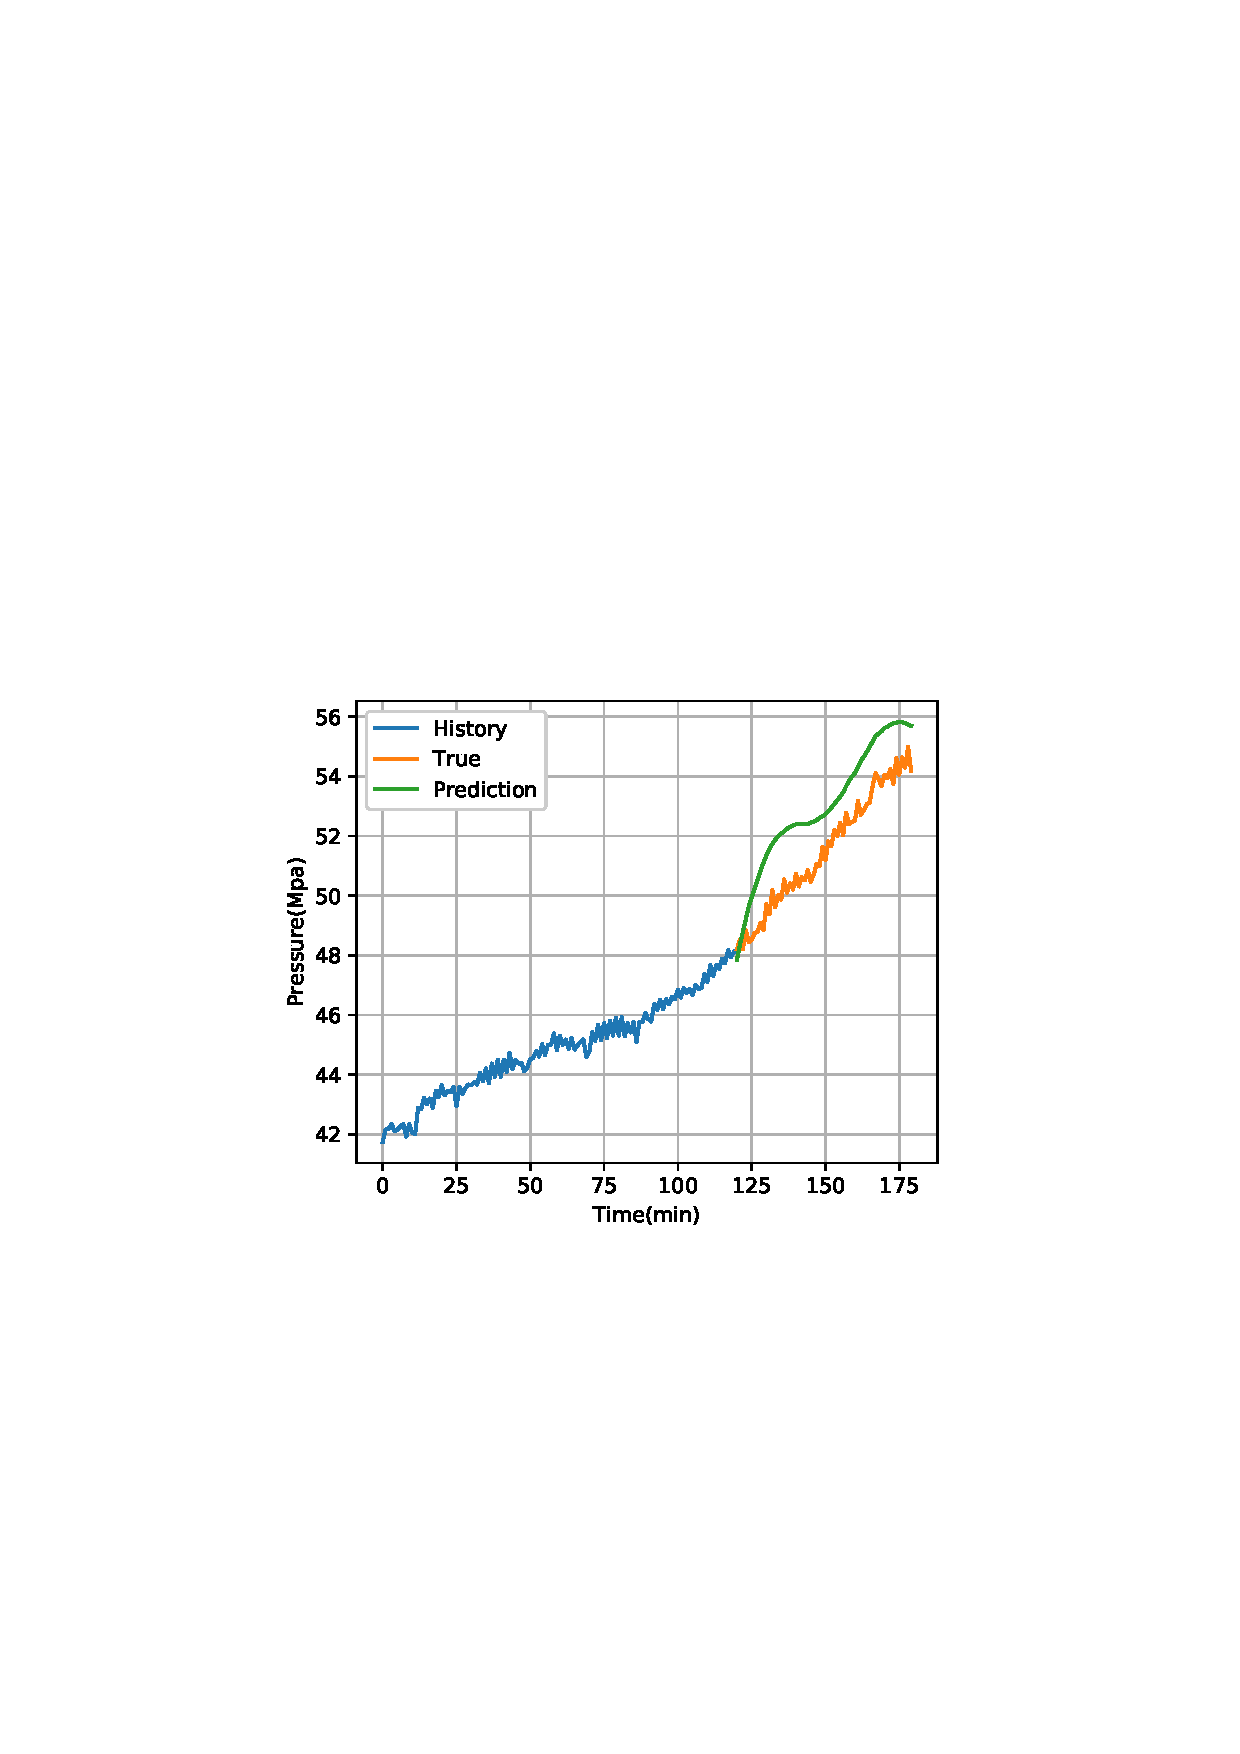
\includegraphics[width=0.49\linewidth,trim=50 0 0 200,clip]{figures/chapter3/predict_cmp/Pressure_MLP_nonsta_rk4_60.pdf}
% \hspace{-18pt}
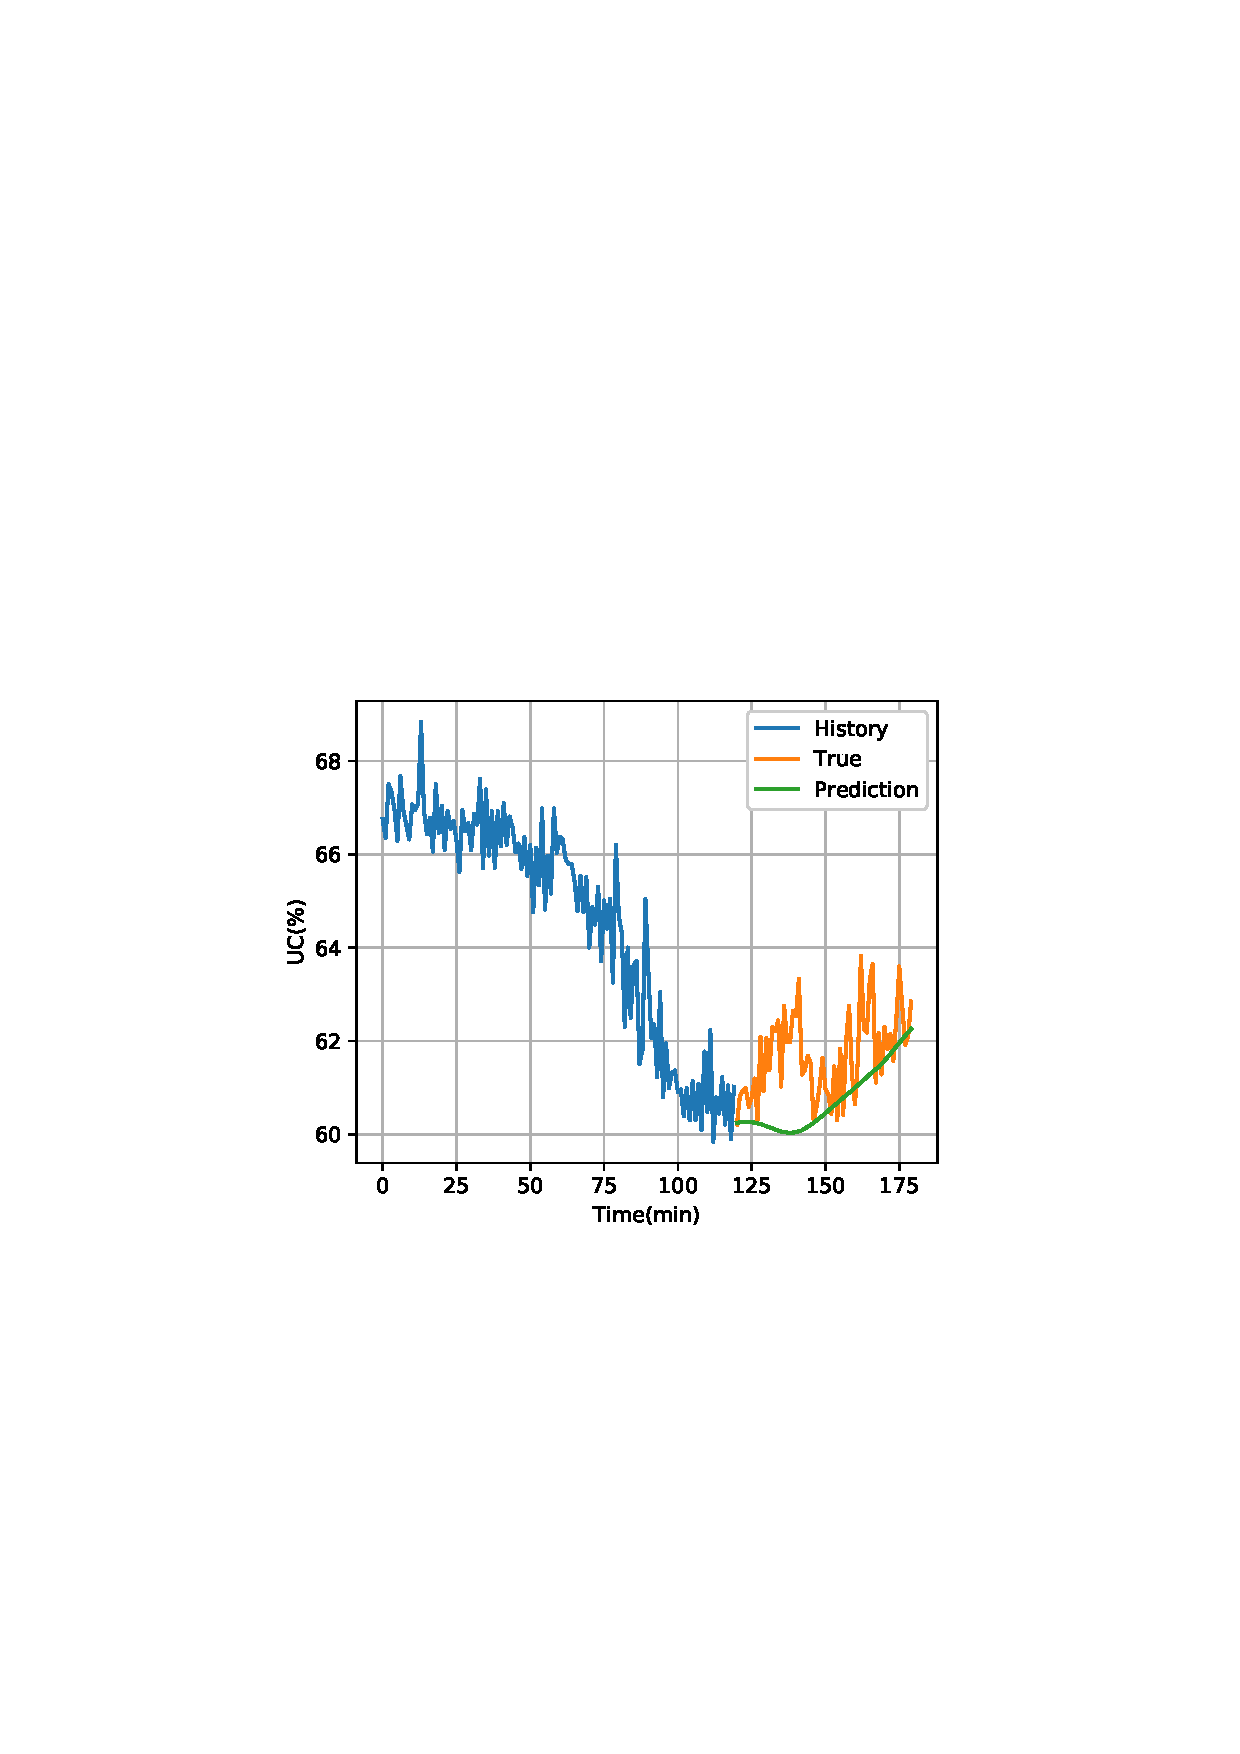
\includegraphics[width=0.49\linewidth,trim=50 0 0 200,clip]{figures/chapter3/predict_cmp/UC_MLP_nonsta_rk4_60.pdf}
%\caption{fig1}
\end{minipage}
}%

% \hspace{-22pt}
\subfigure[非稳定系统+Dopri5求解器]{
\begin{minipage}[t]{\linewidth}
\centering
% \hspace{-22pt}
\includegraphics[width=0.49\linewidth,trim=50 0 0 200,clip]{figures/chapter3/predict_cmp/Pressure_MLP_nonsta_dopri5_60.pdf}
% \hspace{-18pt}
\includegraphics[width=0.49\linewidth,trim=50 0 0 200,clip]{figures/chapter3/predict_cmp/UC_MLP_nonsta_dopri5_60.pdf}
%\caption{fig1}
\end{minipage}
}%
\centering
\caption{不同系统及不同ODE求解器在$L=60$短期预测任务中的性能比较}
\label{fig:predict_cmp_60}
%\vspace*{-0.4cm}
\end{figure}
% k
% \begin{figure}[h]
% \centering
% %\setlength{\abovecaptionskip}{-0.1cm} 
% \subfigure[稳定系统+RK4求解器]{
% \begin{minipage}[t]{0.33\linewidth}
% \centering
% % \hspace{-22pt}
% \includegraphics[width=\linewidth,trim=12 0 0 20,clip]{figures/chapter3/predict_cmp/Pressure_GRU_sta_rk4_60.eps}
% % \hspace{-18pt}

% \includegraphics[width=\linewidth,trim=12 0 0 20,clip]{figures/chapter3/predict_cmp/UC_GRU_sta_rk4_60.eps}
% %\caption{fig1}
% \end{minipage}
% }%
% \hspace{-22pt}
% \subfigure[非稳定系统+RK4求解器]{
% \begin{minipage}[t]{0.33\linewidth}
% \centering
% % \hspace{-22pt}
% 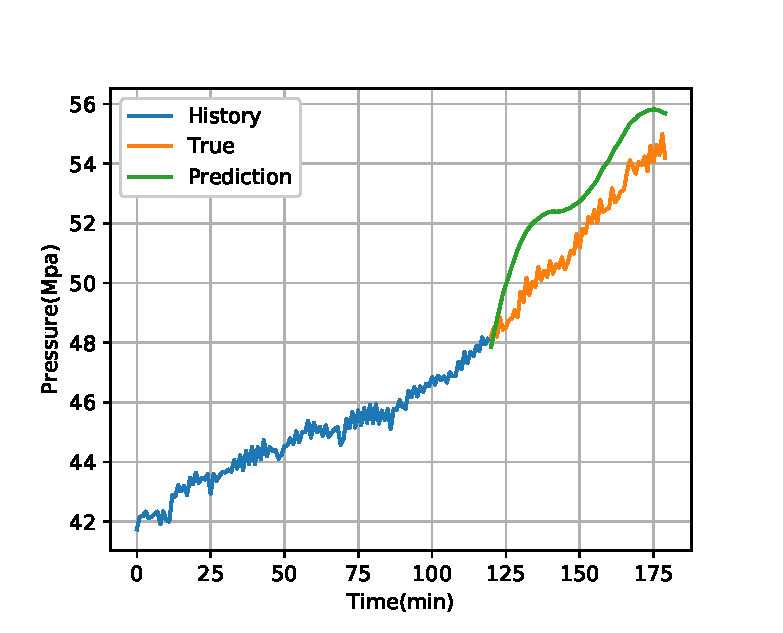
\includegraphics[width=\linewidth,trim=12 0 0 20,clip]{figures/chapter3/predict_cmp/Pressure_MLP_nonsta_rk4_60.eps}
% % \hspace{-18pt}

% 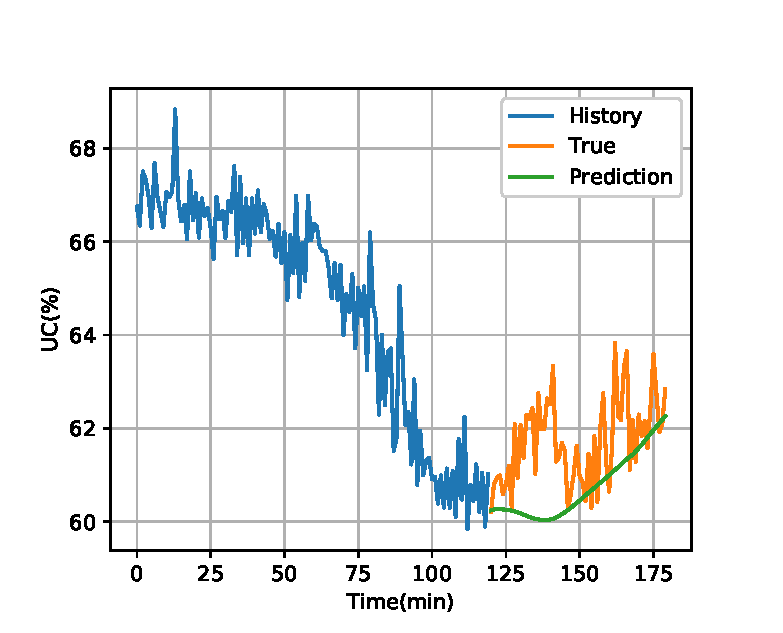
\includegraphics[width=\linewidth,trim=12 0 0 20,clip]{figures/chapter3/predict_cmp/UC_MLP_nonsta_rk4_60.eps}
% %\caption{fig1}
% \end{minipage}
% }%
% \hspace{-22pt}
% \subfigure[非稳定系统+Dopri5求解器]{
% \begin{minipage}[t]{0.33\linewidth}
% \centering
% % \hspace{-22pt}
% \includegraphics[width=\linewidth,trim=12 0 0 20,clip]{figures/chapter3/predict_cmp/Pressure_MLP_nonsta_dopri5_60.eps}
% % \hspace{-18pt}

% \includegraphics[width=\linewidth,trim=12 0 0 20,clip]{figures/chapter3/predict_cmp/UC_MLP_nonsta_dopri5_60.eps}
% %\caption{fig1}
% \end{minipage}
% }%
% \centering
% \caption{不同系统及不同ODE求解器在$L=60$短期预测任务中的性能比较}
% \label{fig:predict_cmp_60}
% %\vspace*{-0.4cm}
% \end{figure}

结果表明,非平稳模型在短期预测任务中的表现优于平稳模型,预测得到的序列相比平稳模型更接近实际系统输出。
% The non-stationary system learns the evolution of internal hidden state which 
% The model with non-stationary system dynamic identifies the system smoothly because the structures constraint hidden state can only change in a continuous and slow form.
% TODO: 真的不想删,但是受篇幅限制暂时注释,以后有机会偷偷补上
此外,由于非稳定系统结构限制了隐状态只能以连续、缓慢的方式变化。该约束符合浓密机系统运行缓慢的特性,等价于减小模型参数的搜索空间,抑制模型过拟合的情况。
图\ref{fig:predict_cmp_200}展示了在长期预测任务($L=200$)中的模型预测结果。
% ($L=500$的类似结果可以在Table~\ref{tab:3_exp_all}中找到)。
\begin{figure}[htpb]
%\setlength{\abovecaptionskip}{-0.1cm} 
\centering
\subfigure[非稳定系统+RK4求解器]{
\begin{minipage}[t]{\linewidth}
\centering
% \hspace{-22pt}
\includegraphics[width=0.49\linewidth,trim=50 0 0 200,clip]{figures/chapter3/predict_cmp/Pressure_MLP_nonsta_rk4_200.pdf}
% \hspace{-18pt}
\includegraphics[width=0.45\linewidth,trim=50 0 0 200,clip]{figures/chapter3/predict_cmp/UC_MLP_nonsta_rk4_200.pdf}
%\caption{fig:subfig_200_nonsta_rk4}
\end{minipage}
\label{fig:subfig_200_nonsta_rk4}
}%
% \hspace{-22pt}

\subfigure[稳定系统+Euler求解器]{
\begin{minipage}[t]{\linewidth}
\centering
% \hspace{-22pt}
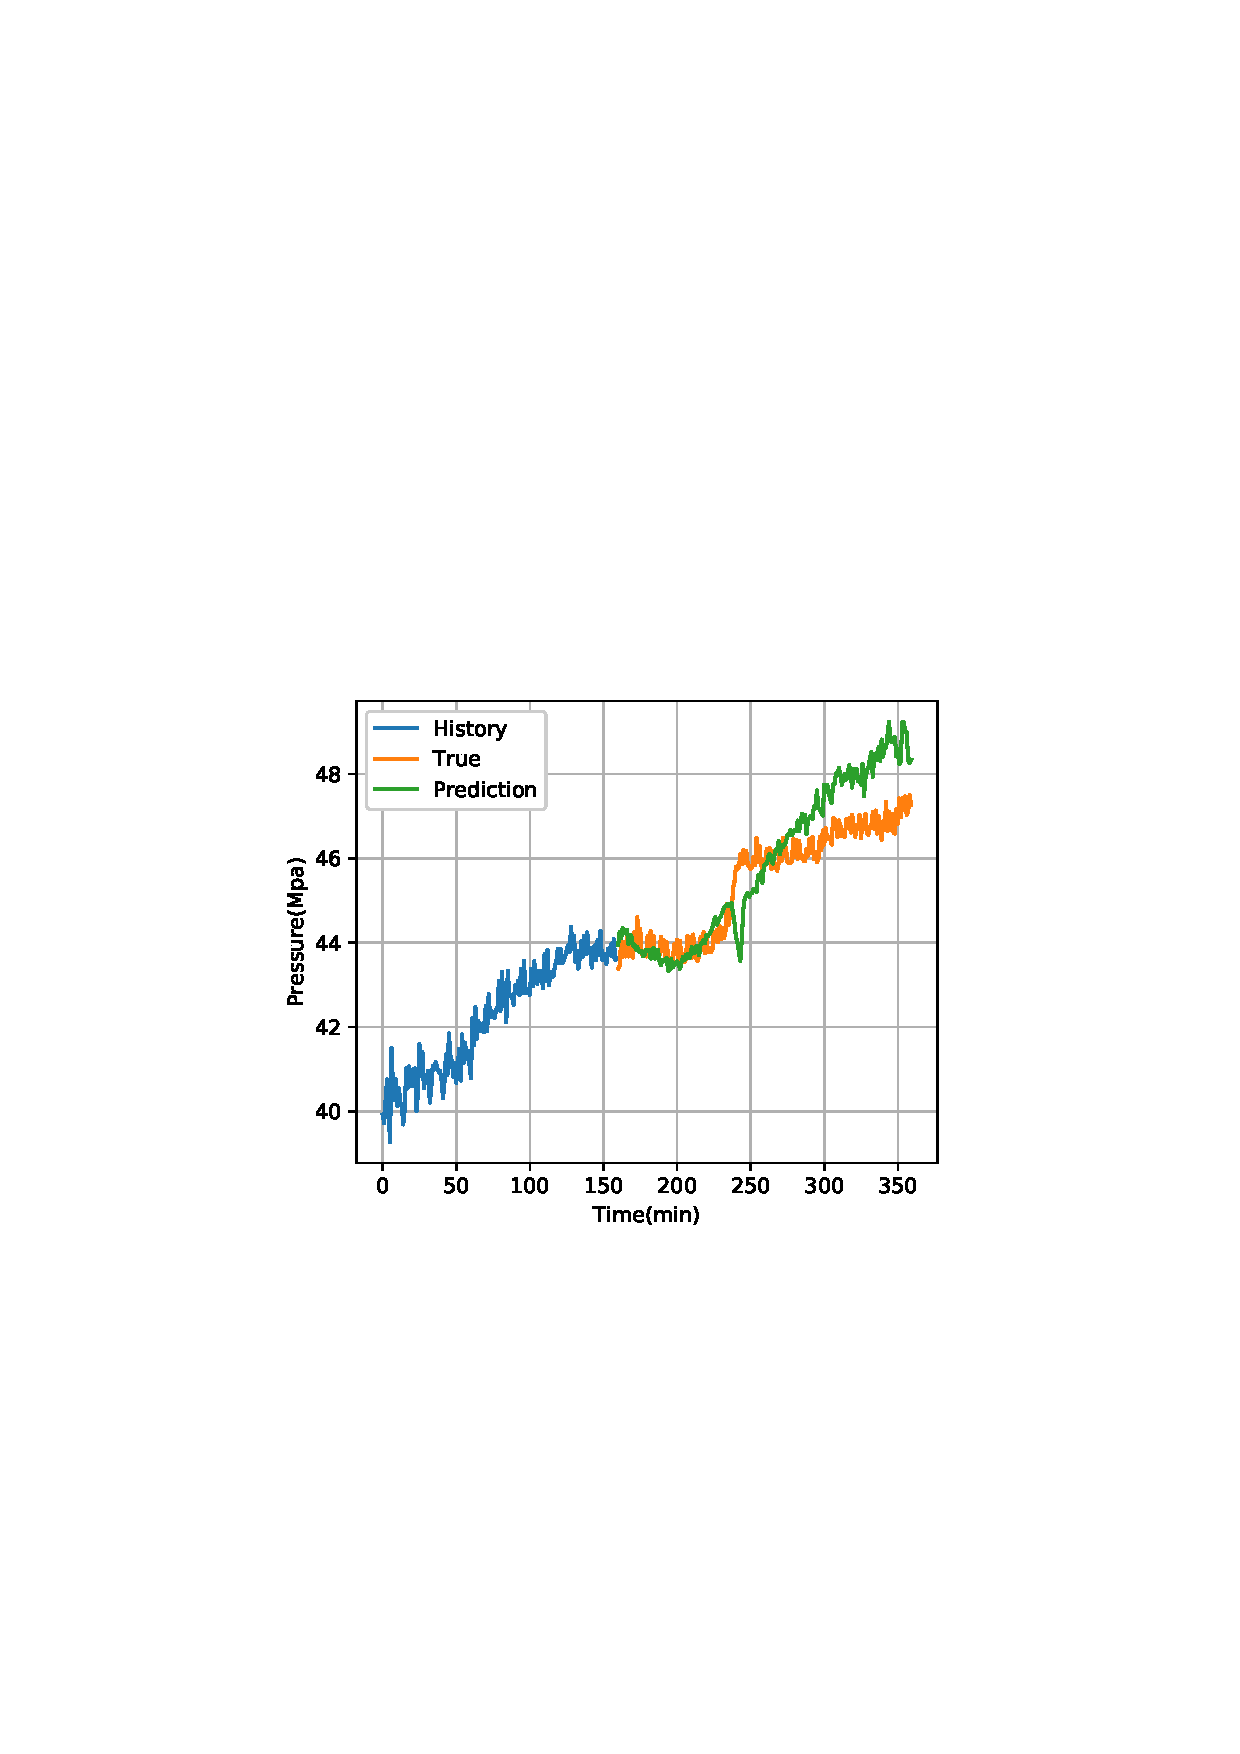
\includegraphics[width=0.45\linewidth,trim=50 0 0 200,clip]{figures/chapter3/predict_cmp/Pressure_GRU_sta_euler_200.pdf}
% \hspace{-18pt}
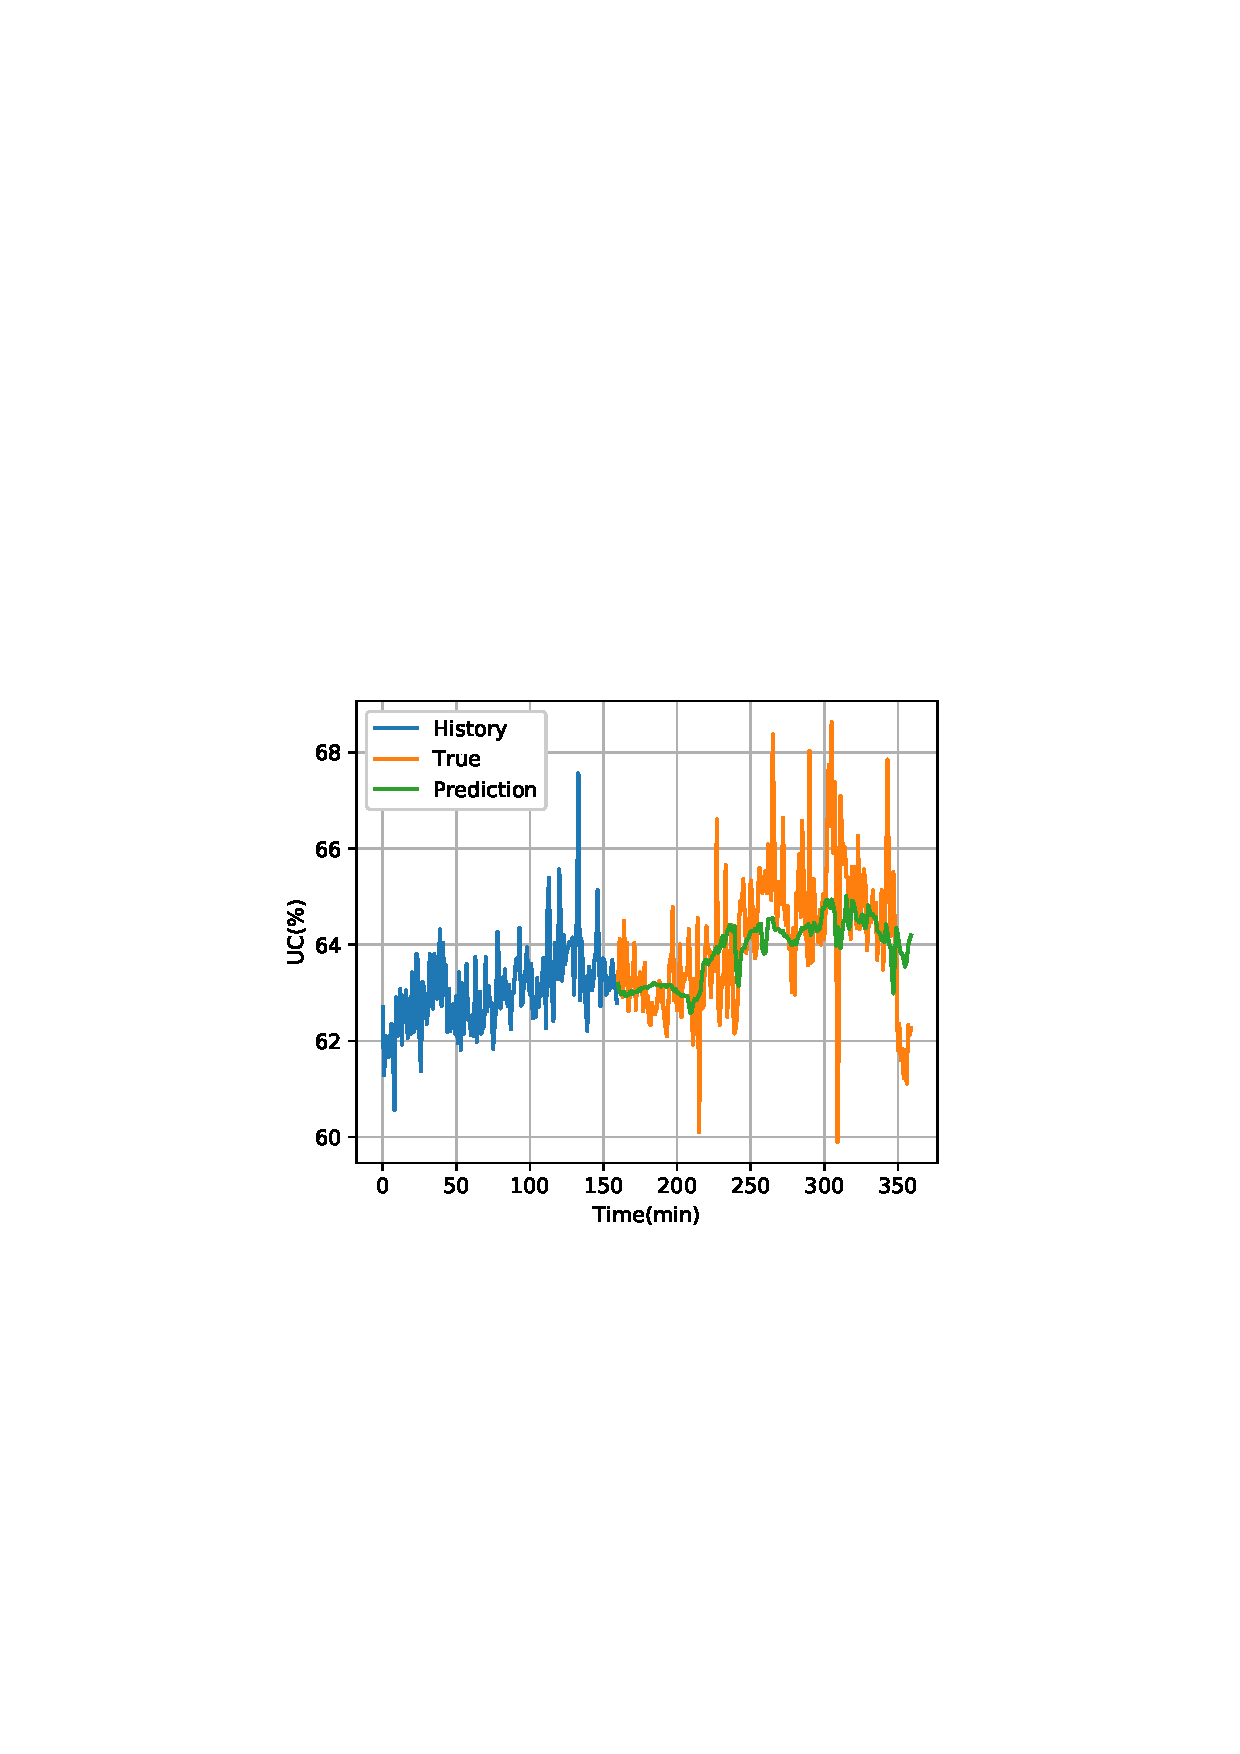
\includegraphics[width=0.45\linewidth,trim=50 0 0 200,clip]{figures/chapter3/predict_cmp/UC_GRU_sta_euler_200.pdf}
%\caption{fig:subfig_200_sta_euler}
\end{minipage}%
\label{fig:subfig_200_sta_euler}
}%

\hspace{-22pt}
\subfigure[稳定系统+RK4求解器]{
\begin{minipage}[t]{\linewidth}
\centering
% \hspace{-22pt}
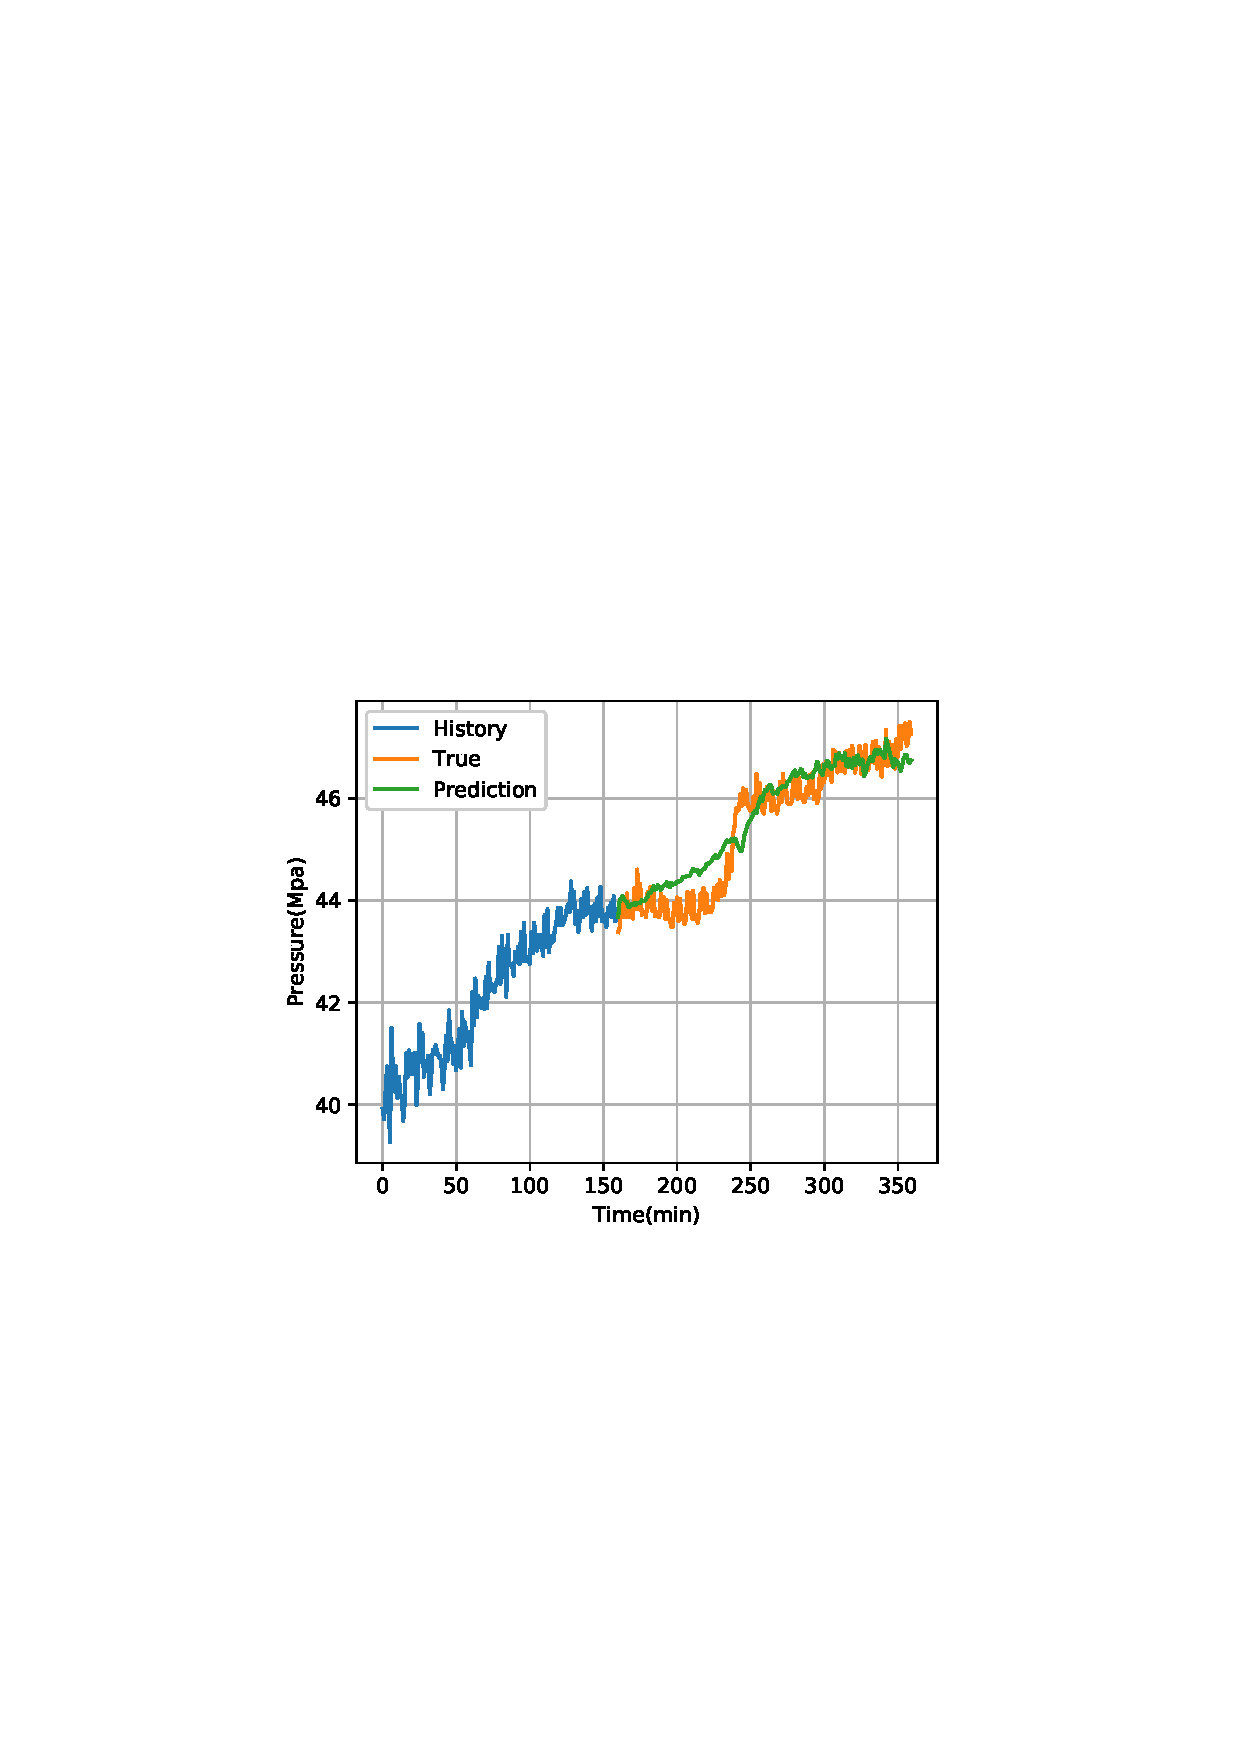
\includegraphics[width=0.45\linewidth,trim=50 0 0 200,clip]{figures/chapter3/predict_cmp/Pressure_GRU_sta_rk4_200.pdf}
% \hspace{-18pt}
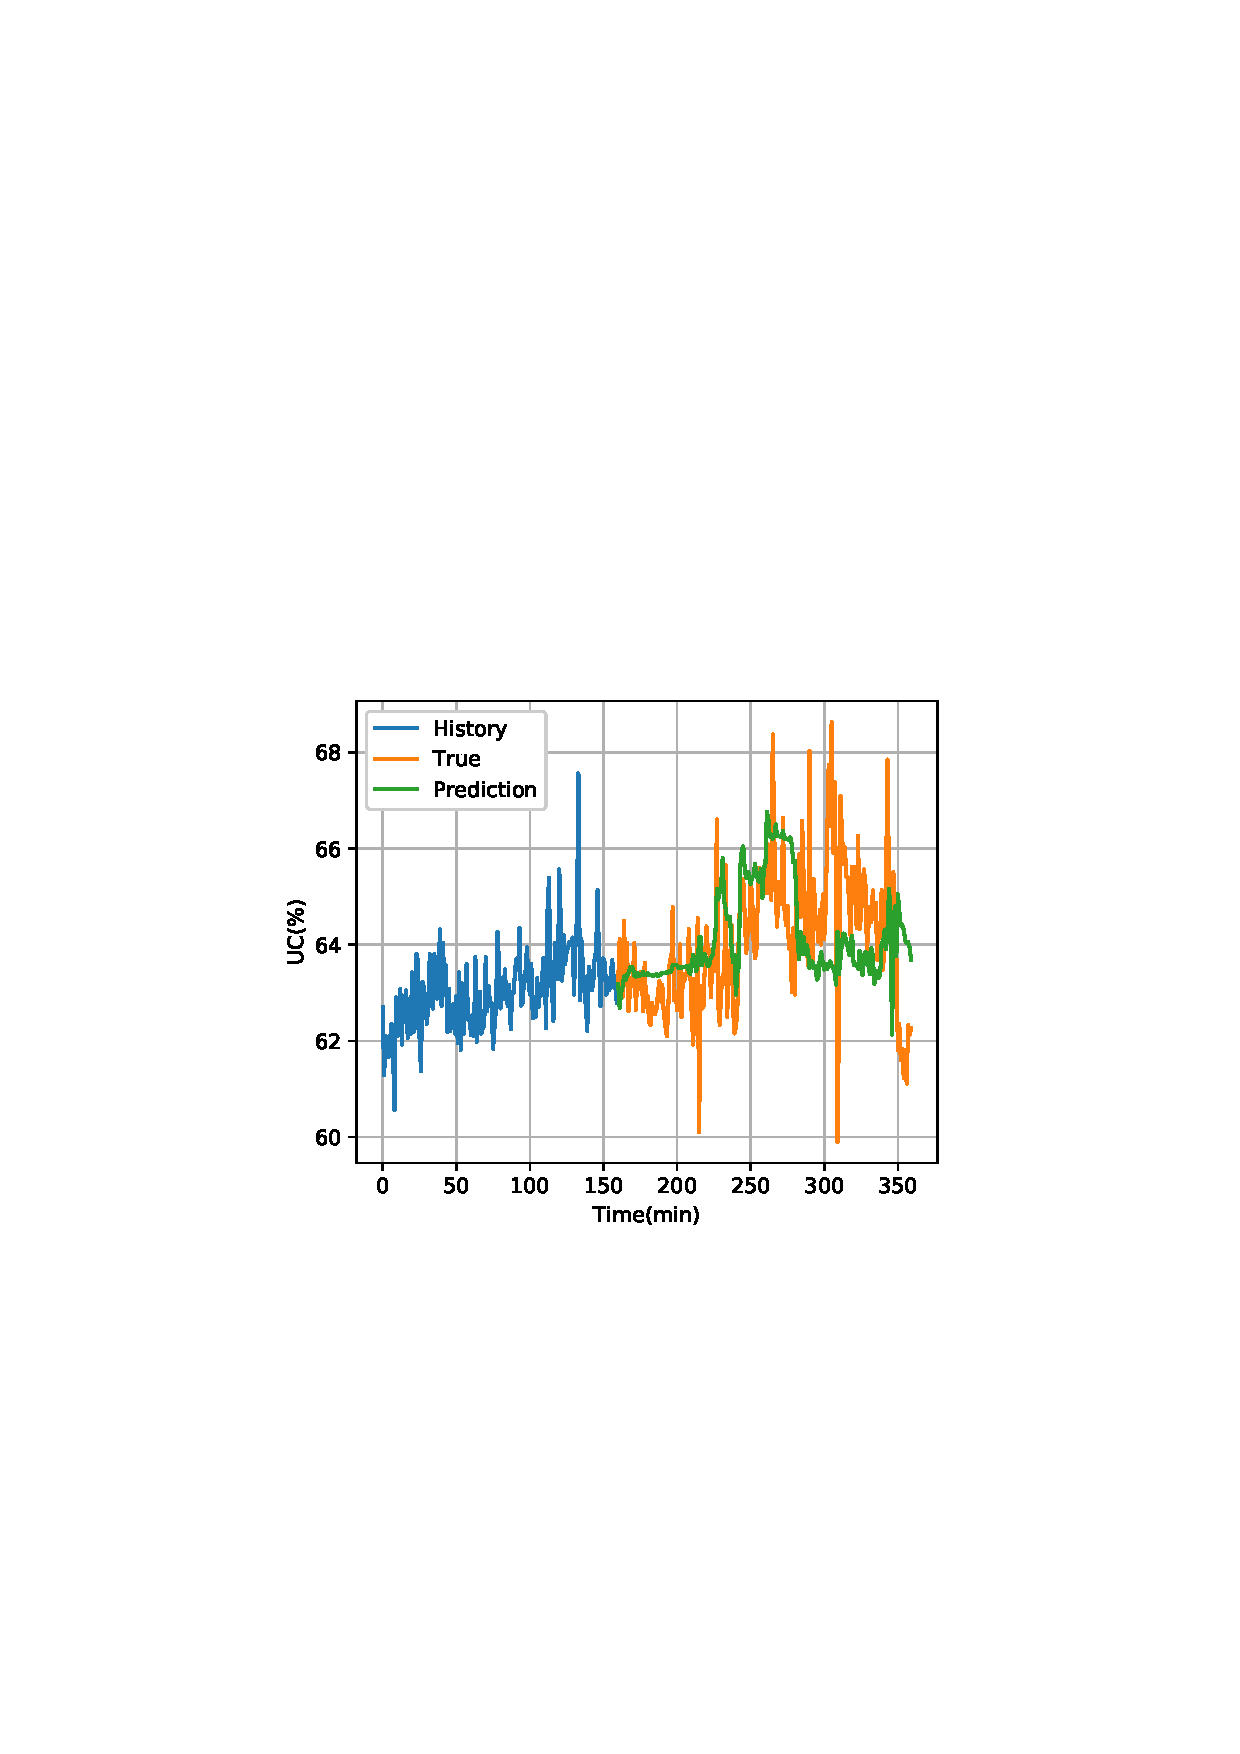
\includegraphics[width=0.45\linewidth,trim=50 0 0 200,clip]{figures/chapter3/predict_cmp/UC_GRU_sta_rk4_200.pdf}
%\caption{fig:subfig_200_sta_rk4}
\end{minipage}%
\label{fig:subfig_200_sta_rk4}
}%
% \subfigure[RNN-sta-Euler]{
% \begin{minipage}[t]{0.31\linewidth}
% \centering
% \includegraphics[width=1.1\linewidth]{figures/chapter3/predict_cmp/UC_RNN_sta_euler_200.eps}
% %\caption{fig2}
% \end{minipage}
% }%
\centering
\caption{$L=200$时不同ODE求解器、不同导数模块下的预测效果对比
} 
\label{fig:predict_cmp_200}
%\vspace*{-0.3cm}
\end{figure}
图中呈现的预测效果与表\ref{tab:3_exp_all}中的结果几乎一致。在长期预测任务中,非平稳模型的RRSE和MSE远远高于平稳模型,模型预测效果较差。
%It is meaningless to compare RRSE indices of results with different $L$, despite the RRSE in the experiments with $L=500$ is lower than $L=200$.
% When , we find that the model with stationary system performs lower prediction error than the non-stationary method.
% The illustrations of predicted results shown in Fig. \ref{fig:predict_cmp_200} and Fig. \ref{fig:predict_cmp_500} demonstrate that the non-stationary model only performs well in early period.
% The illustrations of predicted results shown in Fig. \ref{fig:predict_cmp_200} demonstrates that the non-stationary model only performs well in early period.
% We also illustrate the predicted results with $L=200$ in Fig. .
从图\ref{fig:predict_cmp_60}可以看出,非平稳模型在短期预测问题中展示了更好的预测效果。
而在图\ref{fig:predict_cmp_200}\subref{fig:subfig_200_nonsta_rk4}中,非稳定系统在长期预测时的预测精度显著衰减,且预测偏离程度伴随着预测序列长度的增加而增加。
与之相对地,稳定系统的预测结果是较为稳定的,更接近于系统的真实输出,证明稳定系统在长期预测中准确度更高。
% It is meaningless to compare RRSE indices of results with different $L$.
在由非稳定系统定义的导数模块中,其内部结构导致隐状态在积分过程中是无约束的,状态的取值范围将逐渐扩张。
虽然本章在状态解码器网络中嵌入$\tanh$函数,能够将预测的系统输出限制在合理的范围内,但解码器模块难以学习从极大的隐状态空间到系统输出空间的准确映射。

同样地,图~\ref{fig:predict_cmp_200}也证明了在长期预测问题中,高阶ODE求解器(如4阶Runge—Kutta)能够获得比低阶ODE求解器(如Euler)更好的预测效果,说明微分方程求解的精度会严重影响模型预测的精度,
结果与表\ref{tab:3_exp_all}一致。


% It notes that in the last part of simulation, the predicted system outputs deviate from the real sequences.
% The error is produced because thickening system is a partially observed system.
% Except for known external input or interference in $\b x(t)$, there exist plenty of invisible disturbances which affect the system extremely.
% The negative effects from unknown disturbances make the errors accumulated continuously over a long time period.
% In the long-term prediction task with $L=500$, the stationary model predicts the system outputs well in the former 300 minutes.




% TODO: 这部分也暂时注释,日后有机会再补上
%%%%%%%%%
% seek help: 自回归模型的缺点也是很明显的,每一轮循环的推理必须要在上一轮计算完成之后才能开始,ODE-Net也不例外
% The disadvantage of autogressive model is also obvious that, each round of recurrent inference has to done after the last round finished, and ode-net is no exception.
% One disadvantage for autoregressive model is the recurrent inference must follow by rounds, so does ODE-Net.
%%%%%%%%%

% 结果证实了基本rnn由于忽略了增稠系统的连续时间特性而不能很好地学习系统动力学方程的猜测。




本节额外进行了数组实验,以评估在其他预测长度$L$下,稳定系统和非稳定系统预测的底流浓度误差($\log_{10}{\text{MSE}}$)。
图~\ref{fig:length_cmp}展示了五次重复实验中,底流浓度的预测误差波动情况($\mu \pm 2\sigma$)。
虽然在短期预测任务中非稳定系统精度优于稳定系统,但当$L$超过$120$时,稳定系统表现更优。
% (如$L>100$)。
% 大约,非稳定系统的预测性能差于稳定系统。
\begin{figure}[h]
%\setlength{\abovecaptionskip}{-0.1cm} 
    \centering
    \includegraphics[width=\linewidth,trim=50 0 50 10, clip]{figures/chapter3/length_cmp.pdf}
    \caption{
    % The predicted length $L$ affects average $\log_{10}{MSE} \pm 2\sigma$ range of predicted underflow concentration for both stationary and non-stationary system.
    不同预测长度下稳定系统和非稳定系统的预测精度变化
    }
    \label{fig:length_cmp}
%\vspace*{-0.4cm}
\end{figure}




\subsection{序列编码器的有效性验证及系统时延探究}
\label{sec:3_enc_length}
最后,本节探究了引入序列编码器对于解决长时延系统预测问题的有效性。
% 具体地,该节对比了在引入序列编码器前后以及设定不同编码长度$N$对模型预测精度的影响。
具体地,该节对比了没有序列编码器,以及引入序列编码器并将编码长度$N$设置为不同值时,模型预测精度的变化情况。
特别地,当$N$设置为1时,将序列编码器替换为具有单一隐藏层的神经网络,该网络将单步系统输出$\b y(k-1)$及输入$\b x(k-1)$编码为ODE系统的初始隐状态$\b h(t_0)$。
当$N$为0时,初始状态$\b h(t_0)$被设定为可学习的初始隐状态\cite{Demeester2020SystemIW}或零向量,与历史系统轨迹无关。

% 在不同的预测序列长度$L=60$、$200$和$500$的三个实验中,我们测试了不同的$N$对预测精度的影响。
该实验仍然在$L=60$、$200$和$500$三种情况下比较不同初态估计方法对预测精度的影响。
在$L=60$的实验中,导数模块被为非平稳系统。
当$L=200$和$500$时,导数模块定义为带有GRU单元的稳定系统。
六组实验中,均采用四阶龙格-库塔求解器求解ODE方程。



\begin{table}[t]
\caption{不同初始隐状态 $\b h(t_0)$生成方法对于预测精度的影响}
\label{tab:seq2seq_cmp}
\centering
% \renewcommand{\arraystretch}{1.5}
\begin{tabular}{c|cc|cc|cc}
    \toprule
\multirow{2}{*}{$N$}                                                & \multicolumn{2}{c|}{\begin{tabular}[c]{@{}c@{}}$L=60$ \\ (120 分钟)\end{tabular}}                 & \multicolumn{2}{c|}{\begin{tabular}[c]{@{}c@{}}$L=200$ \\ (400 分钟)\end{tabular}}                  & \multicolumn{2}{c}{\begin{tabular}[c]{@{}c@{}}$L=500$ \\ (1000 分钟)\end{tabular}}                \\
\cline{2-7}
                                                                                     & RRSE                & MSE                 & RRSE                & MSE                  & RRSE                & MSE                  \\ \hline
160                                                                               & 3.11                & 9.08                &  \uline{\textbf{3.56}} & 34.13                & 1.61                & 35.88                \\
80                                                                                &  \uline{\textbf{3.10}} &  \uline{\textbf{8.97}} & 3.58                &  \uline{\textbf{32.92}} &  \uline{\textbf{1.61}} &  \uline{\textbf{34.88}} \\
40                                                                                & 3.19                & 8.99                & 3.65                & 36.07                & 1.71                & 41.26                \\ \hline
1                                                                                 & 4.06                & 10.71               & 4.97                & 51.09                & 1.77                & 63.56                \\ \hline
$N=0$,$\b h(t_0)$作为学习参数                  & 5.26                & 20.68               & 4.84                & 58.68                & 1.77                & 63.91                \\ \hline
$N=0$,令  $\b h(t_0)=\b 0$                                                                   & 5.26                & 23.11               & 5.84                & 64.49                & 1.77                & 63.53                \\ 
\bottomrule
\end{tabular}
\end{table}
从表\ref{tab:seq2seq_cmp}中的结果可以看出,相比于完全忽略历史系统输出($N=0$),引入序列编码器并利用历史运行轨迹构建常微分方程的初态能够获得更好的预测精度。
直觉上的解释为,待预测的系统未来输出与历史系统轨迹具有很强的统计相关性,从后者提取的特征对于序列预测具有重要意义。利用序列编码器能够将此部分相关性嵌入在ODE初态中。
根据实验发现,被编码序列的最优长度约为$N=80$,这与浓密机系统存在2至3小时时延的先验经验几乎一致。

另外,引入序列编码模块的收益在短期预测任务更加明显。
随着被预测序列长度的增加,引入序列编码器带来的优势也随之降低。

\subsection{探究序列插值阶数的对预测精度的影响}
% 本小节进行消融实验以探究不同离散输入序列进行插值的方法是否对预测精度产生影响。
本小节进行消融实验以探究不同离散输入序列插值方法对预测精度的影响。
测试对象包括四种不同阶数的样条插值方法,最终比较模型在不同预测长度的预测精度。
预测长度设置、导数形式、以及ODE求解器选择均与实验\ref{sec:3_enc_length}一致。
% The recurrent cell in experiment is RNN and the schema for solving ODE is RK4 uniformly.
表~\ref{tab:interolopation_cmp}所示结果表明,采用高阶样条插值时的精度将稍优于低阶插值。
\begin{table}[h]
\centering
%\setlength{\abovecaptionskip}{-0.1cm} 
\caption{不同序列插值方法对预测精度的影响}
\renewcommand{\arraystretch}{1.5}
\label{tab:interolopation_cmp}
\begin{tabular}{c|cc|cc|cc}
\toprule
 \multirow{2}{*}{模型}         & \multicolumn{2}{c|}{\begin{tabular}[c]{@{}c@{}}$L=60$ \\ (120 分钟)\end{tabular}}                 & \multicolumn{2}{c|}{\begin{tabular}[c]{@{}c@{}}$L=200$ \\ (400 分钟)\end{tabular}}                  & \multicolumn{2}{c}{\begin{tabular}[c]{@{}c@{}}$L=500$ \\ (1000 分钟)\end{tabular}}                 \\
    & RRSE                 & MSE                  & RRSE                 & MSE                   & RRSE                 & MSE                   \\ \hline
三次样条插值     &  \uline{\textbf{3.083}} & \uline{ \textbf{8.565}} & \uline{ \textbf{3.581}} & 32.90                & 1.615                & \uline{\textbf{ 34.88}} \\
二次样条插值 & 3.097                & 8.993                & 3.593                &\uline{ \textbf{32.585}} &\uline{ \textbf{1.613}} & 36.741                \\
线性插值   & 3.098                & 8.999                & 3.763                & 33.530                & 1.627                & 37.778                \\
零阶样条插值      & 3.115                & 9.050                & 3.791                & 33.585                & 1.628                & 37.695                \\ \bottomrule
\end{tabular}
%\vspace*{-0.4cm}
\end{table}
该结果说明本章所研究的膏体浓密机系统为复杂非线性受控系统,受控输入信息对于预测系统输出是十分重要的。
高阶样条插值方法能够更充分地利用相邻位置输入信号的相关特征,相比于低阶插值方法,能够更精确地对空白区域进行插值填充。

\section{本章小结}
\label{sec:conc}
本章针对高时延工业多输入输出系统预测问题,
提出了一种基于ODE-Net的连续时间网络模型,该模型由序列编码器、状态解码器和导数模块三部分组成,模型的内部计算过程包括历史序列编码、离散输入序列插值以及常微分方程求解三部分,模型能够从连续时间域角度拟合复杂系统的动态过程。
本章采用膏体浓密机系统运行数据集进行实验,以探究导数模块的不同定义方式、ODE求解器选择、离散序列插值阶数、序列编码长度对于预测精度的影响。
% 在真实膏体浓密机系统运行数据集,本章进行了大量实验对所提出模型的各个部分进行研究,包括平稳系统和非平稳系统的选择以及不同ODE求解器的设定。
结果表明,非平稳系统在短期预测任务中的表现优于平稳系统。
% 但是,非平稳模型由于存在累加计算,会造成隐状态的波动范围过大,进而导致长期预测性能较差。
在实际应用中,当构建基于模型的反馈控制器时,可使用非平稳系统作为短期预测模型辅助控制器输出。
但是,非平稳模型在长期预测时隐状态的波动范围过大且存在较大的累积误差,
而平稳系统通过修改导数模块结构,避免了隐状态漂移问题,因此在长期预测中表现较好。
当需要具有稳定鲁棒的系统识别模型进行长期预测时,如系统仿真或控制器测试,平稳系统模型是更好的选择。
同时,通过消融实验表明模型中引入序列编码器和并行三次样条插值能够有效改善模型精度。


% 在工业数据分析领域,面向不均匀采样数据的分析与预测是极其常见的。虽然本章所用数据集的采样间隔是均匀的,由于本文所述模型是基于ODE-Net进行构建的,具有连续时间域的系统学习及表示能力,因此该方法可以很自然地处理不均匀数据。
% 该问题值得在今后的工作中被进一步的验证。
% 另外将本章方法扩展为概率模型和时变模型,以辅助确定复杂系统中的未知噪音和不确定性,也是未来极具价值的研究方向。


% %第四章

\chapter{基于自跳跃常微分方程网络的连续时间周期跳变系统建模}
周期跳变系统在现实生活中随处可见,其运行过程具有周期循环性。
连续时间周期跳变系统指各阶段依周期转换,
% 且每个周期内,各阶段之间按特定顺序进行切换。
且系统在不同阶段会呈现不同动态特性的连续时间跳变系统。
例如,洗衣机启动后将按程序设定,周期性地在进水,洗涤,排水,甩干等各个阶段之间循环运行,直至最后关机。
冰箱和空调在工作期间会在运行(压缩机开启)和待机(压缩机关闭)两种状态之间不断切换。
% 在一些自然界中其他的物理过程,也存在类似的系统,例如建筑物内的空调制冷系统、交通流量和季节变化等。
% 生产生活中的一些其他过程也存在类似特性,例如交通流量和季节变化等。
% % 在使用自回归模型对具有周期多阶段特性的系统进行预测时,我们希望模型能够自动地在特定时刻进行状态转移。
% 在对城市交通流量或某产品销量进行预测时,其流量或销量通常伴随着特定的日期和季节进行改变,并且其周期长度相对稳定,模型能够较容易地识别各时刻下被预测对象所处的当前阶段。
% 而对于一些复杂工业系统,其各阶段的持续时间可能受到系统内部和外部多个变量的影响。
% 例如系统的外部输入、当前内部状态、环境条件等。
% 为了优化此类系统的运行参数与运转模式,
利用历史数据建模其阶段跳变过程与各阶段内的动态模型参数对于优化此类系统的运行参数与运转模式是极其重要的。
% 对于此类带有多阶段特性的复杂工业系统,想要采用单一模型学习具有不同阶段特性的动态并且实现精确的系统预测与仿真是极其困难的。

然而,在对复杂跳变系统进行建模时会面临两大技术难题。
首先,跳变系统通常有多个阶段,每个阶段内系统将呈现完全不同的非线性特性,且各个阶段的持续时间可能同时受到内部因素和外部因素的影响\cite{WANG2022111790}。现有的跳变系统参数估计方法\cite{balenzuela2022parameter}通常依赖于对系统结构以及持续时间分布的先验认知,这需要大量的领域专家知识作为支撑。
另外,对于带有多输出项的工业系统,其输出项中可能同时存在稳定和非稳定过程\cite{nason2006stationary}。
目前为止,现有的未经过特定设计的辨识模型难以解决此类带有混合时序特性的系统学习任务。

% 为了实现上述目标,模型需要解决两个问题。
% 首先,模型需要根据系统的外部输入以及系统状态,识别在当前时刻系统所处的阶段。
% 另外,模型需要能够准确地识别系统在各阶段内的独立动态特性。
针对上述技术难题,本章提出了自跳跃常微分方程网络(Autonomous jump ordinary differential equation net, AJ-ODE-Net)以学习同时带有稳定和非稳定输出的连续时间周期跳变系统。
该模型是一种新颖的连续时间深度学习模型,能够从非均匀采样的系统历史轨迹进行学习。
% 该框架主要用于建模具有周期性多阶段转换的多输入输出系统,利用数据驱动的方式从系统输出序列中学习系统不同阶段的动态特性。
训练完成后,对于给定的系统外部输入,模型能够给出开环的仿真预测结果。
为了学习系统在不同阶段的动态特性,模型包含多个层次常微分方程网络(Hierarchical ODE-Nets ,H-ODE-Nets)。
该网络是一种双层扩展的常微分方程网络,能够建模同时带有稳定输出和非稳定输出的动态系统。
为了实现开环预测时的阶段自转移,本章对原始训练数据进行了阶段类别标注,并在模型中引入阶段转换预测器学习每个阶段的持续时间。
阶段转换预测器由多个持续时间预测器构成,每个预测器能够预估当前所处阶段的持续时间。在开环预测和仿真中,阶段转换预测器能够作为H-ODE-Nets的调节器,在每个时间点指派合适的H-ODE-Net进行系统输出的预测,并自发地转移至下一阶段。

% 为了使模型能够从数据中自动地学习各阶段内的系统动态特性,针对待预测系统输出同时存在非稳定过程和稳定过程的问题,引入分层常微分方程网络。
% (hierarchical ODE-Nets, H-ODE-Nets)实现对系统多维输出的混合学习。

% 因此,在本章提出的AJ-ODE-Nets模型中,参考了有限状态机的基本思想,构建了可学习的阶段转换模块。
同时为了给定AJ-ODE-Net的状态初值,
本章基于编码器解码器(Encoder-Decoder)框架,构建了两个AJ-ODE-Net分别用于历史数据的编码以及在给定的系统输入序列下以开环的方式预测系统的未来输出。
本章提出了基于编码器解码器(Encoder-Decoder)框架的预测模型。该模型包含两个AJ-ODE-Net,编码AJ-ODE-Net用于编码历史数据以给定解码AJ-ODE-Net的初态,解码AJ-ODE-Net能够在给定的系统输入序列下以开环的方式预测系统的未来输出。

% 除此之外,本章引入样条插值算法,以连续化离散的输入序列并作为AJ-ODE-Net模型的输入。
最后,本章将所述模型及编解码预测框架应用于具有典型周期多阶段特性的膏体制备水泥添加过程的预测与仿真问题中。
% 在给定系统的多变量输入数据下,包括热负载以及环境温度,模型能够仿真系统的运行过程并准确地预测系统能耗,能耗预测误差小于5\%。
在给定系统的多变量输入数据下,包括浓密机底流浓度以及底流流量,模型能够仿真系统的运行过程并准确地预测膏体浓度及水泥消耗,其中水泥量消耗量的预测误差小于5\%。
进一步地,利用模型的仿真功能能够优化膏体制备过程的浓度设定参数,仿真实验表明利用优化之后的浓度设定值能够在保证膏体浓度满足要求的前提下,显著减少螺旋给料器的开机频率以及水泥消耗6-25\%。
% 本章所述模型能够有效地模拟制冷系统的运行,预测其功率消耗以及服务器进气口温度。

% Addressing the challenges and problems mentioned above, we propose AJ-ODE-Nets, a novel framework for modeling and identifying the non-linear dynamics at different stages in periodic operational systems. The framework is specifically capable of capturing physical dynamics thanks to the implementation of ODE-Net, a neural network based on ODE. The framework is expected to learn the multivariate inputs-ouputs system in a data-driven way, by feeding several sequences of sensory data as training data. Once trained, the model is able to realize real time predictions according to the multivariate inputs. Modeling multi-stage periodic systems requires two principal realizations, one for the stages prediction, one for dynamical characteristics identifications of different stages. 





% With this purpose, in the design of AJ-ODE-Nets, a selective structure is considered.
% In terms of learning dynamical characteristics at different stages,
% the framework contains several hierarchical ODE-Nets (H-ODE-Nets), and the number depends on the observed system stages. H-ODE-Nets can be seen as an extension of ODE-Net, which can deal with both stationary and non-stationary sequences. 
% In terms of learning the system transitions during operation, a stage transition predictor is included in the AJ-ODE-Net module, which can infer the transfer actions from a sequence of observation data, specifically, when and how to change to other tendency during system operation. In order to train the stage transition predictor, the observation data has been labeled previously in a conditional data range, based on prior knowledge of the system operational specifications. During predictive range, the stage transition predictor serves as the governor to appoint to the suitable H-ODE-Net, so as to let the system run across different working stages periodically. Adaptive smoothing algorithm is introduced to impute missing data as well, it can handle nonlinear and irregularly sampling data, which is practical in dealing with sensory data from IoT systems. The AJ-ODE-Nets framework has been further implemented in a running data center with contained structure, to simulate the cooling system operations. 

本章研究主要包含三方面贡献,概括如下:
\begin{itemize}
    % \item 首先,本章将原始的ODE-Net模型扩展到H-ODE-Net模型,能够学习同时带有稳定和非稳定时间序列输出的动态过程。
    \item 为了辨识连续时间跳变系统,本章提出了一种新颖的深度学习模型——自跳跃常微分方程网络模型。该模型能够实现
    (1)在集成化的网络中学习系统的多阶段动态,(2)在长序列开环预测中实现阶段自转移。
    % \item 其次,本章针对具有周期多阶段特性的动态系统,开创性地提出了AJ-ODE-Nets模型,该模型通过引入阶段转换预测器学习系统的周期性阶段转换以及采用多个H-ODE-Nets学习不同阶段内的系统动态特性。
    \item 为了学习同时包含稳定和非稳定项的多输出系统,本章结合每个输出项的统计特性,引入H-ODE-Net以改善长期预测中两种输出项的预测精度。
    % \item 本章所述模型成功应用于某一工业制冷系统的预测与仿真问题中,该模型能够在给定热负载功率下,准确地预测制冷系统的功率消耗以及冷气温度变化,利用该仿真模型能够优化制冷系统的工作温度设定值,进而优化制冷系统整体能耗约6-25\%。
    \item 本章提出的AJ-ODE-Net模型成功应用于膏体制备系统的预测与仿真问题中,该模型能够在给定浓密机出料浓度与流量下,准确地预测系统的水泥消耗以及膏体浓度变化,利用该仿真模型能够优化控制螺旋给料器启停的浓度设定值,在控制螺旋给料器开机频率的同时,显著减少水泥消耗6-25\%。
\end{itemize}
% Two main contributions are devoted to this study, summarized as follows::
% \begin{itemize}
%     \item First, we extent the original vanilla ODE-Net to the Hierarchical ODE-Net (H-ODE-Net), which is able to learn the stationary and non-stationary time series data simultaneously.
%     \item Second, we propose AJ-ODE-Nets framework, targeting at learning periodic multi-states systems in data-driven way. AJ-ODE-Nets disposes of several H-ODE-Nets to automatically learn dynamic characteristics at different states, along with a stage transition predictor to learn the transition actions during operation. 
% \end{itemize}

本章正文内容的结构组织如下:
\ref{sec:4_notations}节给出了周期性多阶段系统预测问题中的变量符号定义以及形式化描述。
% 本章\ref{sec:h-ode}节介绍了分层常微分方程网络的定义及结构,以及如何将其用于学习同时带有稳定和非稳定时间序列输出的动态过程。
\ref{sec:4_ajode}节介绍了AJ-ODE-Net模型的基本结构,并详细阐述了
如何采用分层常微分方程网络学习同时带有稳定和非稳定时间序列输出的动态过程,以及如何构建连续时间域下的跳变系统状态转移方程。
% 最后给出了基于AJ-ODE-Net模型的编码器解码器框架及其训练方法
\ref{sec:4_encoder_decoder}节介绍了基于双AJ-ODE-Net模型的编码器解码器框架,并详细介绍了AJ-ODE-Net的初态求解方法。
\ref{sec:4_loss_function}节给出了用于训练持续时间预测器和预测模型的损失函数。
% 关键模块结构和持续时间预测器的损失函数定义等内容。
% 本章\ref{sec:4_encoder_decoder}给出了基于AJ-ODE-Net模型的编码器解码器框架及其训练方法。
\ref{sec:4_evalutaion}节将介绍利用所述框架建模膏体制备系统的水泥添加过程。
% 模型能够根据系统的热负载输入对其功耗以及出气口气体温度变化进行模拟预测,
同时,介绍如何利用辨识模型优化制备系统的浓度设定值以降低设备的重启频率并降低水泥消耗。
最后,\ref{sec:4_conclusion}节对本章工作进行总结,并对AJ-ODE-Net模型的未来研究方向以及在其他领域的应用做出了展望。


% The paper is organized as follows: related work on time series prediction for industrial systems, and for multi-state systems are summarized in Sec.~\ref{sec:review}. Then, preliminary in Sec.~\ref{sec:preliminary} describes the basic theory used in this study. After that, in Sec.~\ref{sec:methodology_dfaode}, the proposed framework AJ-ODE-Net is detailed in terms of data processing, structure of key modules and training for loss functions. In practice, the proposed framework is applied to simulate several working variables of a cooling system in real data centers. Two use cases are included, one for real time estimation of the energy consumption based on system inputs and environmental condition, and the other takes advantage of the integrated prior knowledge, simulations are conducted to optimize the consumption by varying configurations. In the end, Sec.~\ref{sec:4_conclusion} concludes the entire work and discuss the potential future work.
\section{问题形式化描述}
\label{sec:4_notations}
% 在本章中,标量和向量在形式上分别用小写字母和粗体小写字母表示,例如$y, \boldsymbol y$。
假设输入输出数据由传感器观测得到,并带有时间戳$t_i\in \mathbb{R}$。
因此,从系统中采集的带有非均匀采样间隔的离散输入序列和输出序列可表示为:
$\boldsymbol X_{1:I},\boldsymbol Y_{1:I}= ((t_1,\boldsymbol x_1,\boldsymbol y_1),(t_2,\boldsymbol x_2, \boldsymbol y_2),\cdots,(t_I,\boldsymbol x_I,\boldsymbol y_I))$。
%with each $t_i\in \mathbb{R}$ the timestamp of the system input and output, and $t_{0}<\cdots<t_{n}$.
% we define $\boldsymbol y_i$ as the $i$-th vectorial variable in a discrete sequence. 
相应的,定义$\boldsymbol x(t_i)=\boldsymbol x_i$ 以及 $\boldsymbol y(t_i)=\boldsymbol y_i$。
其连续时间过程可表示为$\boldsymbol x:\left[t_{1}, t_{I}\right] \rightarrow \mathbb{R}^{M}$ 和 $\boldsymbol y:\left[t_{1}, t_{I}\right] \rightarrow \mathbb{R}^{N}$。
为了便于后文描述,本章将$\boldsymbol y:\left[t_{1}, t_{I}\right]$简化为$\boldsymbol Y_{t_1:t_I}$。


连续时间跳变系统(Continuous-time Jump System,CTJS)由多个连续时间子系统组成,其内部阶段转换受有限状态过程控制\cite{8709809}。
典型的连续时间跳变系统定义如下:
% As an important class of dynamical systems, CTJS arises in many applications, such as failure prediction\cite{9165930}, control applications\cite{pmlr-v120-jansch-porto20a}, and state estimation\cite{8709809}.
% 作为一种特殊的动态系统,CTJS系统广泛应用于各类应用中,如故障预测\cite{9165930}、系统控制\cite{pmlr-v120-jansch-porto20a},以及状态估计\cite{8709809}。
\begin{equation}
    \dot{\boldsymbol h}(t)=\mathcal{F}_{\sigma(t)}(\boldsymbol h(t), \boldsymbol x(t),
    \label{equ:ctjls}
\end{equation}
% where $\sigma(t)\in\{0,1\cdots N-1\}$ is a finite-state step process and $\boldsymbol{x}(t)$ is system inputs with the Lipschitz continuity.
% With different $\sigma(t)$, the non-linear system dynamics $\mathcal{F}_{\sigma(t)}$ are distinct.
% Compared to a general continuous-time markov jump system whose state $\sigma(t)$ is a markov process, this study assumes that the transition of $\sigma(t)$ is deterministic and circular.
% Specifically, in a continuous-time periodic jump non-linear system, the piece wise constant state $\sigma(t)$ jumps in a cycle order $\{0,1,\cdots,N-1,0 \cdots\}$.
% The sojourn time between jumps depends on the trigger thresholds according to prior knowledge about the system.
% To distinguish between the state in a system and the hidden state in a recurrent neural network, we name the system state $\sigma(t)$ as the \textbf{\textit{stage} in this paper.
其中$\sigma(t)\in\{0,1\cdots,N-1\}$为一有限状态集下的跳变状态,$\boldsymbol{x}(t)$为满足利普希茨连续的系统输入。
为了明确区分跳变系统中的状态变量$\sigma(t)$以及循环神经网络中的隐状态,本章将跳变系统状态$\sigma(t)$命名为阶段。
在一般的连续时间马尔科夫跳变系统中,系统阶段$\sigma(t)$的变化遵循马尔科夫过程。
而本章假设阶段变量$\sigma(t)$的转移过程是依周期的且循环过程是确定的,
分段恒定的$\sigma(t)$在循环$\{0,1,\cdots,N-1,0 \cdots\}$中不断变化。
阶段跳跃之间的停留时间取决于由系统本体属性决定的触发条件。
因此本文所关注的系统也称为连续时间周期跳变系统(Continuous-time periodic jump system)。
% 基于模型驱动的参数估计或系统辨识方法有时很难被应用于复杂的跳跃系统中,因为实际的动态行为很难被识别。为了从现有的输入输出数据中学习CTJS,以前的研究假设了系统的先验结构,并采用了EM算法(balenzuela2022parameter}、顺序蒙特卡洛(SMC)(6859280)和变异推理(opper2007variational)等方法来估计模型参数。

同本文第三章,本章要解决的问题仍为根据系统的历史数据信息和以及系统的未来序列输入,开环地预测系统的未来输出。
具体地,本章将给定数据的时间范围$[t_1:t_{I+L}]$分为两部分:条件范围$[t_1:t_{I}]$和预测范围$[t_{I}:t_{I+L}]$。
%Given $\{{\boldsymbol{X}}_{t_{1}:t_{I+L}}, {\boldsymbol {Y}}_{t_{1}:t_{I+O}}\}$, the system inputs and system outputs in time range $[t_1:t_{I+O}]$,
% , where ${\boldsymbol y}^i_{1:I+O}=[{\boldsymbol y}^i(t_1),\boldsymbol y^i(t_2),\dots,{\boldsymbol y}^i(t_{I+O})]$ and ${\boldsymbol y}^i(t_j)$ is the $j-th$ value in $i-th$ system outputs series collected at time $t_j$ . 
模型通过给定条件范围$[t_1, t_I]$下的系统输入和系统输出生成初始状态,然后利用训练得到的跳变模型\equref{equ:ctjls}对预测范围$[t_{I}, t_{I+L}]$下的系统输出进行预测,如式~\ref{equa:problematique}所示:

\begin{equation}
\label{equa:problematique}
    \hat{\boldsymbol Y}_{t_{I}:t_{I+L}} = f(\boldsymbol Y_{t_{1}:t_{I}}, \boldsymbol X_{t_{1}:t_{I+L}};\boldsymbol \zeta) 
\end{equation}
公式中$\hat{\boldsymbol Y}_{t_{I}:t_{I+L}}$表示预测范围内的模型输出。 
$\boldsymbol Y_{t_{1}:t_{I}}$表示在条件范围内系统的历史输出。
$\boldsymbol X_{t_{1}:t_{I+L}}$表示完整时间范围内的系统输入,包括历史输入和未来输入部分,其未来输入也被称为协变量\cite{Wu2020}。
% 该系统输入在时间序列预测领域经常被称为协变量\cite{Wu2020}。
$\boldsymbol \zeta$表示利用数据集训练的模型可学习参数。
本章的目标为通过优化$\boldsymbol \zeta$以最小化$||\hat{\boldsymbol Y}_{t_{I}:t_{I+L}}-\boldsymbol {Y}_{t_{I}:t_{I+L}}||^2$。
值得注意的是,上述过程仍为开环预测,模型预测过程中无法收到来自系统输出的反馈。
% Where $\hat{\boldsymbol Y}_{t_{I}:t_{I+L}}$ is the estimated outputs in predictive range. $\boldsymbol Y_{t_{1}:t_{I}}$ represents the historical system outputs in conditional range.
% $\boldsymbol X_{t_{1}:t_{I+L}}$ is the system inputs of whole range that involve both historical and predictive parts.
% $\boldsymbol \zeta$ is the learnable parameters of model trained jointly from all available datasets. \\

% The formulation in Eq.~\eqref{equa:problematique} is similar to the time-series forecasting problem, which focuses on extracting temporal information and predicting the future outputs given historical observed targets and covariates \cite{Lim2021}.
% \eqref{equa:problematique}所示的形式化描述类似于时间序列预测问题。
% Time series forecasting methods are employed for extracting temporal information and predicting the future outputs given historical observed targets and covariates \cite{Lim2021}.
% However, the research scope of this paper is more related to the field of system modeling/identification , which focuses on modeling the dynamics of the system.
% The historical system observations herein are mainly utilized to provide an accurate initial state.
% With an inferred initial state, the model can predict the system outputs in open loop, based on the given system inputs in a predictive range. 
% The length of the predictive range is determined according to the length of the simulation we want to make.
% Taking the studied cooling system simulation as an example, we can theoretically feed arbitrary long heat loads as inputs and the model will simulate the corresponding temperature variation in that predictive range.
% 以制冷系统为例,可以将任意长度的热负载序列数据作为模型输入,模型能够仿真预测区间下的温度变化。
% 因此,在训练阶段,预测范围长度与条件范围长度是一致的,为800s。
% 在实验一中,预测范围的长度为30分钟,本章考虑到由于误差累积导致的相位偏差,因此没有采用点对点式的评估指标,而是采用预测累积能耗的估计误差对模型可靠性进行评估。

% However, when there is no feedback from system outputs, the long-term open-loop simulations are unreliable for a stochastic or uncertain system.
% In Section \ref{sec:case-study1}, although the length of the predictive range is altered to 30 minutes, 
% we considered the accumulated estimated error of phases positions and give up the point-to-point evaluation and seek other evaluation indicators


% \section{自跳跃常微分方程网络及编码器-解码器预测架构}
\section{自跳跃常微分方程网络}
\label{sec:4_ajode}
\subsection{基于分层ODE-Net的稳定及非稳定输出混合建模}
大部分工业系统的输出是多维度的,不同维度输出的时序统计特性存在一定差异,某些输出项为均值、方差恒定的稳定过程,某些输出项为均值、方差不断变化的非稳定过程。
对于同时含有稳定和非稳定输出的混合过程进行建模学习具有一定难度,当前主流的基于深度学习的序列预测领域并未针对该类系统开展研究。
针对该问题,本章提出分层常微分方程网络(Hierarchical ODE-Net, H-ODE-Net)以建模同时包含稳定过程和非稳定过程的复杂系统。

具体地,H-ODE-Net将三个ODE-Net集成为双层结构(L-1和L-2)。
% Modeling hybrid processes with both stationarity and non-stationarity properties is another challenge for industrial systems, as existing methods normally target one situation. With this in mind, Hierarchical ODE-Net (H-ODE) is proposed to model a system containing non-stationary and stationary processes simultaneously. In 图.~\ref{fig:AJ_ODEs}, there are $N$ number of H-ODE-Net embedded in the AJ-ODE-Net module, and only one will active at specific time point $t$, based on state variable $\sigma(t)$. In detail, H-ODE hierarchically integrates a two-level structure (L-1 and L-2) with three ODE-Nets.
% to deal with the mixed situations mentioned above.
%The learned continuous-time predictive model is named Hierarchical ODE-Net which hierarchically integrates a two-level ODE-Net.
图~\ref{fig:H_ode}展示了H-ODE-Net中三个ODE-Net之间的连接方式。
\begin{figure}
    \centering
    \includegraphics[width=\linewidth]{figures/chapter4/Hode.pdf}
    \caption{H-ODE-Net结构图示}
    %\caption{An H-ODE-Nets consists of three ODE-Net. The high-level ODE-Net estimates the derivative of latent state according to external inputs. By integrating the ODE equation with high-level ODE-Net, the solved $\boldsymbol h(t)$, accompanied with external inputs $\boldsymbol x(t)$ and duration time of current stage $T(t)$, is fed into two low-level ODE-Nets to estimate the derivatives of system outputs. The predictions of system outputs at arbitrary time points $t_x$ can be solved by integrating the low-level ODE-Nets.}
    \label{fig:H_ode}
\end{figure}
在L-1层中的一个ODE-Net用于根据外部输入对隐状态的导数进行建模。利用实时求解出的$\boldsymbol h(t)$、外部输入$\boldsymbol x(t)$和当前阶段持续时间$T(t)$,对由L-1中的ODE-Net定义的常微分方程进行积分。
在L-1层中的一个ODE-Net
用于根据外部输入对隐状态的导数进行建模。
利用实时求解出的$\boldsymbol h(t)$、外部输入$\boldsymbol x(t)$和当前阶段持续时间$T(t)$对隐状态导数进行建模。
% 由L-1中的ODE-Net定义的常微分方程进行积分。
对L-1中定义的常微分方程进行积分解出的$\boldsymbol h(t)$将作为L-2中两个ODE-Net的输入,并分别用于求解稳定系统输出项和非稳定系统输出项,表示为$\boldsymbol y(t)=[\boldsymbol y_s(t), \boldsymbol y_{ns}(t)]$。
% 最终,可以解出任一时间点$t_x$下的预测结果。

% 图.~\ref{fig:H_ode} illustrates the connections between three ODE-Nets within H-ODE. The L-1 contains one ODE-Net to model the derivative of
% %The high level part of H-ODE-Net is an ODE-Net that 
% latent state according to external inputs. By integrating the ODE equation with ODE-Net of L-1, the solved $\boldsymbol h(t)$, combined with external inputs $\boldsymbol x(t)$ and duration of current stage $T(t)$, are fed into L-2 ODE-Nets to model the derivatives of stationary and
% %the stationary system outputs and 
% non-stationary system outputs, denoted as $\boldsymbol y(t)=[\boldsymbol y_s(t), \boldsymbol y_{ns}(t)]$ respectively. The predictions at arbitrary time points $t_x$ are solved in the end. 
%and the low-level part consists of 
%and only one particular H-ODE-Net corresponding to $s(t)$ may be utilized to make prediction at time point $t$.
%To utilize one model to predict a system involving the non-stationary and stationary process simultaneously, we propose a hierarchical ODE-Net whose three ODE-Nets predict the derivative of latent state, the derivative of stationary system outputs and the derivative of non-stationary system outputs respectively.

其中,L-1中的ODE-Net为第三章所述的稳定结构,由门控循环单元(GRU)网络实现:
% The ODE-Net in L-1
% %for modeling latent state 
% is stationary and implemented by stationary Gate Recurrent Unit (GRU) network\cite{Demeester2019}:
\begin{equation}
    \label{equ:dh}
    \frac{d \boldsymbol{h}(t)}{dt} = \frac{1}{\mu(t)}*\left[\text{GRU}(\boldsymbol{x}(t), \boldsymbol{h}(t),\text{sigmoid}(T(t)), \theta^\mathcal{H}_{\sigma(t)}) - \boldsymbol{h}(t)\right]
\end{equation}
其中$\mu(t)$表示原始数据集的平均采样间隔均值。
稳定的GRU网络将预测的隐状态变量$\boldsymbol{h}(t)$的变化表示为稳定过程,并将其上下界限制在$(-1,1)$范围内。


% where $\mu(t)$ denotes the mean of sampling intervals in entire dataset.
% Stationary GRU network treats the predicted latent state $\boldsymbol{h}(t)$ as a stationary process and constrains the outputs within range $(-1,1)$. 
% In comparison to stationary model which produces stabilized latent state, incremental models(non-stationary model) suffers from potentially linearly growing state, which is ill-suited for modeling long-term stationary time series~\cite{Demeester2019}.

% unit root problem and bring in long-term prediction.
% potentially linearly growing state is ill-suited for modeling stationary time series
%The low-level ODE-Nets

L-2中的两个ODE-Net被分别用于建模稳定和非稳定的系统输出。
其中被用于建模非稳定输出的导数网络采用非稳定增量形式预测输出$y_{ns}(t)$ :

% The two ODE-Nets in L-2 are designed to %is utilized to model the instant derivatives for system outputs in using two ODE-Nets 
% cover both stationary and non-stationary cases.
% % In this study, consumed power of cooling system $y_1(t)$ and cooling capacity $y_2(t)$ are categorized as stationary outputs, $\boldsymbol{y}_{s}(t)=[y_1(t), y_2(t)]^T$.
% % The inlet temperature of cooling system $y_3(t)$ is categorized as non-stationary outputs, $\boldsymbol{y}_{ns}(t)=[y_3(t)]^T$. 
% The one for $y_{ns}(t)$ is employed by implementing non-stationary incremental neural network:
% %One of low-level ODE-Nets, implemented by an non-stationary incremental neural network, is employed to model non-stationary outputs:
\begin{equation}
    \label{equ:dyns}
    \frac{d \boldsymbol{y}_{ns}(t)}{dt} = \text{NN}(\boldsymbol{x}(t),\boldsymbol{y}_{ns}(t), \boldsymbol{h}(t), \text{sigmoid}(T(t)), \theta^{\mathcal{Y}^{ns}}_{\sigma(t)})
\end{equation}

另一个ODE-Net类似于L-1中的ODE-Net,由稳定的GRU模型构建,用于预测系统的稳定输出$y_s(t)$:
% Another ODE-Net for $y_s$ is similar with the one in L-1, which is implemented by a stationary GRU module
% to model stationary outputs:
\begin{equation}
    \label{equ:dys}
    \frac{d \boldsymbol{y}_{s}(t)}{dt} = \frac{1}{\mu(t)}*\left[\text{GRU}(\boldsymbol{x}(t),\boldsymbol{y}_s(t), \boldsymbol{h}(t), \text{sigmoid}(T(t)), \theta^{\mathcal{Y}^{s}}_{\sigma(t)}) - \boldsymbol{y}_s(t)\right]
\end{equation}

对于L-2中的两个ODE-Net,均将系统处于当前阶段的持续时间$T(t)$作为特征输入,辅助估计 $\boldsymbol{y}(t)$的导数。
$\{\theta_i^{\mathcal{Y}^{ns}},\theta_i^{\mathcal{Y}^{ns}},\theta_i^{\mathcal{H}}\}_{i=1}^N$是模型中的可学习参数。
% In both L-1 and L-2, duration of current stage $T(t)$, accumulated since the start of each stage, is chosen as a feature to estimate the derivatives of $\boldsymbol{y}(t)$. 
% $\{\theta_i^{\mathcal{Y}^{ns}},\theta_i^{\mathcal{Y}^{ns}},\theta_i^{\mathcal{H}}\}_{i=1}^N$ are learnable parameters.
%because the periodic system has similar behaviors in the same stages and similar time points.
% employed to model stationary outputs and non-stationary outputs separately:
% hypothesize that it is there- fore more naturally suited to deal with stationary data.
% Two low-level ODE-Nets are 

一般情况下,从传感器测量得到的数据通常是离散的且带有不规则分布的缺失值。例如可能存在某一时刻$i$,两区间$t_i-t_{i-1} \neq t_{i+1}-t_{i}$或者存在$\boldsymbol x(t_i)$存在,而$\boldsymbol y(t_i)$缺失的情况。
本章采用第三章\ref{sec:3_interpolation_training}中介绍的并行可微插值方法,将离散的控制输入序列插值为连续时间信号并作为ODE-Net的输入。
% 因此需要实现面向离散序列输入的连续化插值方法,将离散和采样不规则的数据格式转换为连续时间格式。
% 为了实现该目标,有多种方法可以实现,如高斯过程\cite{li2016scalable},核方法\cite{shukla2018interpolation}或样条插值\cite{kidger2020neural}。本章参考\cite{kidger2020neural}采用三次样条插值方法。
% Generally speaking, data samples got from sensory measure system are commonly discrete and irregularly distributed with proportional missing values. 
% It may exist one timestamp $i$, the interval $t_i-t_{i-1} \neq t_{i+1}-t_{i}$, or $\boldsymbol x(t_i)$ exists while $\boldsymbol y(t_i)$ is missing and be represented as \textit{Null} in dataset.
% % As an instance, some
% ODE-Net takes only continuous data as input, therefore, the processing module is in charge of implementing interpolation methods to transfer discrete and irregular data samples to continuous format. There are many options, such as Gaussian processes\cite{li2016scalable}, kernel methods\cite{shukla2018interpolation} or natural cubic spline \cite{kidger2020neural}, appropriate interpolation method is free to apply in consideration of concrete situations.



% \subsection{基于循环神经网络的初始状态编码}
\subsection{微分方程状态空间定义及阶段自转移}
% \label{sec:dfa-odenet}
% \subsection{状态定义}
% 部分工业系统存在多阶段、非确定和多物理过程混合等复杂特性。对这类系统进行高精度、高鲁棒的建模是一项具有挑战性的任务。
% 在本章研究中,为了能够使模型准确地预测多阶段系统的阶段转换时刻以及预测系统输出,本章提出了AJ-ODE-Net模型。
为了使辨识模型准确地预测周期跳变系统中的阶段转换以及建模各个阶段下的系统输出,本节在H-ODE-Net基础上提出了自跳跃常微分方程网络模型。
具体地,我们首先利用系统先验知识构建系统的多阶段转换过程,对于每个阶段引入一个H-ODE-Net以学习系统在该阶段内的动态特性,通过对训练集中的序列数据进行阶段变量标注,可以定向地训练各个H-ODE-Net的参数。
同时,在预测框架中引入阶段转换预测器学习预测每个阶段的持续时间。
在测试阶段,阶段预测器可以作为不同H-ODE-Net的调节器,实现不同阶段之间的自动转移。
图~\ref{fig:AJ_ODEs}简要介绍了AJ-ODE-Net的主要组件及其结构。
\begin{figure}
    \centering
    \includegraphics[width=0.9\textwidth]{figures/chapter4/Jump-ODEnet.pdf}
    \caption{AJ-ODE-Net 模型结构}
    \label{fig:AJ_ODEs}
\end{figure}

在图\ref{fig:AJ_ODEs}中,AJ-ODE-Net模型嵌入了$N$个H-ODE-Net模块,根据状态变量$\sigma(t)\in \{0,\cdots,N-1\}$,在同一时刻只使用一个H-ODE-Net用于系统预测。
相比于普通的ODE-Net仅建模系统隐状态的导数,
AJ-ODE-Net将隐状态扩展为四个参数,即$\boldsymbol{S}(t) = [\boldsymbol h(t), \boldsymbol y(t), \sigma(t), T(t)]$,
其中四项分别为\textbf{系统隐状态}、\textbf{预测的系统输出}、\textbf{系统所处的当前阶段}和\textbf{处于当前阶段已经持续的时间}。
这种定义形式能够覆盖连续时间跳变系统中建模系统输出变化以及阶段变量变化所需的全部信息。
AJ-ODE-Net可以看作是ODE-Net的扩展形式,其状态的计算与更新均在连续时间域下进行。
给定时间点$t$和无穷小时间步长$\tau$,状态更新方程
如\equref{equ:stage_trans_predic}所示:

% For attention, even though there are several ODE-Nets as dynamical representations for available stages, only one ODE-Net is active during processing, appointed by stage predictor. Therefore, AJ-ODE-Net can still be seen as an extended version of ODE-Net. Different to ODE-Net shown in 式 \eqref{equ:ode_net} , which contains only self-governed hidden state predicted from input, AJ-ODE-Net extend the hidden state to four arguments to cover enough dynamical variations in the system. Specifically, the calculation and update of hidden states are continuous-time processes, denoted by $\boldsymbol{S}(t) = [\boldsymbol h(t), \boldsymbol y(t), \sigma(t), T(t)]$, represent the \textbf{predicted hidden states}, \textbf{predicted system outputs}, \textbf{current stage} and \textbf{duration of current stage} respectively. %given current timestamp. 

% The updating can be seen as a differential process given time point $t$ and infinitesimal time step $\tau$, as illustrated by 式~(\ref{equa:states_updates}):

\begin{align}
% \label{equa:states_updates}
\boldsymbol S(t+dt)=\left[
\begin{aligned}
&\left .\begin{aligned}
&\boldsymbol{h}(t) + \frac{d \boldsymbol{h}(t)}{\tau} *dt  \\
&\boldsymbol{y}(t) + \frac{d \boldsymbol{y}(t)}{\tau} *dt  \\
\end{aligned}
\right \}\quad \text{见公式} \eqref{equ:dh}\text{, }\eqref{equ:dyns}\text{, 和 }\eqref{equ:dys}
\\
&s(t+dt) =
\left\{
\begin{aligned}
\sigma(t) + 1 \text{ mod } N,\quad &T(t)>=\hat {\tau}_{\sigma(t)}(t) \\
\sigma(t), \quad &\text{else}
\end{aligned}
\right.\\
&T(t+dt) = 
\left\{
\begin{aligned}
0,\quad &T(t)>=\hat {\tau}_{\sigma(t)}(t) \\
T(t)+dt, \quad &\text{else}
\end{aligned}
\right.\\
\end{aligned}
\right]
\label{equ:stage_trans_predic}
\end{align}

% 对于复杂的周期多阶段系统而言,很难用统一的模型拟合系统的所有阶段,在长期预测问题中该问题更加明显。
对于周期稳定、各个阶段持续时间不变的系统,可以将系统的运行过程分解为若干区间,分别学习各阶段内的系统动态特性。
但是,更普遍的情况是,系统中各阶段的持续时间会受到系统内部和外部多个变量的影响。
为了使模型适用于系统中各阶段持续时间不稳定的情况,本章引入“持续时间估计器”,通过学习的方式,在预测时预估每个阶段的持续时间,并辅助模型判断是否应切换到下一阶段。

具体地,我们结合周期性多阶段系统中的先验知识,可以很容易地设计描述系统在各个阶段之间的状态转换过程。
% 基于该AJ模型,可以建立一个基于持续时间估计器的阶段转换预测器。
% 从给定的数据集中学习相邻阶段之间的转换规则,使系统在运行时切换到不同的H-ODE-Net进行预测,将系统输出预测和阶段识别进行解耦。
对于$t$时刻的连续时间状态$\boldsymbol{S}(t)$ , 
$\sigma(t)\in\{0,\dots,N-1\}$表示系统当前所处阶段,$T(t)$表示系统处于阶段$\sigma(t)$的持续时间。

对于\equref{equ:stage_trans_predic}描述的状态演化过程,本章基于多层感知器实现了与当前阶段变量${\sigma(t)}$绑定的持续时间估计器$\hat{\tau}_{{\sigma(t)}}$来预测当前阶段的最终持续时间。预测器的输入为当前隐状态$\boldsymbol{h}(t)$和外部输入$\boldsymbol{x}(t)$:
% 对于系统运行过程中可能出现的每个阶段$\sigma(t)$,基于多层感知器分别构建持续时间预测器,预测器的输入为当前隐状态$\boldsymbol{h}(t)$和外部输入$\boldsymbol{x}(t)$。
% $\hat{\tau}_{\sigma(t)}$为持续时间估计器预估的$\sigma(t)$阶段将会持续的时间。
\begin{equation}
\hat{\tau}_{\sigma(t)}(t)=\text{NN}\left([\boldsymbol{h}(t), \boldsymbol{x}(t)], \phi_{\sigma(t)}\right)
\end{equation}
其中$\phi_{\sigma(t)}$为可学习参数,当满足$T(t)\geq\hat{\tau}_{\sigma(t)}(\boldsymbol{h}(t),\boldsymbol{x}(t))$时,模型将切换到下一阶段$(\sigma(t)+1)\text{ mod } N$并将$T(t)$复位为0。
% where $\phi_{\sigma(t)}$ is learnable parameters.
% % 图.re.~\ref{fig:dt_label} illustrates the predicting and supervised signals of duration time predictors.
% %the accumulative duration of current stage satisfies 
% $T(t)\geq\hat{\tau}_{\sigma(t)}(\boldsymbol{h}(t),\boldsymbol{x}(t))$, the model will switch to the next stage $(\sigma(t)+1)\text{ mod } N$ and reset $T(t)$ to zero.
\section{基于编码器解码器结构的微分方程网络初值估计与序列预测}
\label{sec:4_encoder_decoder}
% 求解ODE方程前,需要确定初值。
在周期跳变系统的开环预测问题中,确定系统当前所处的相位,包括识别当前系统所处阶段以及当前阶段已经持续的时间是极其重要的。
% Meanwhile, the observation space of complicated system is always incomplete, subject to the limitation of monitoring techniques. Thus, to make accurate prediction, the model needs to 
% infer the uncertain information by embedding the historical trajectories in the initial state.
与此同时,受限于测量技术及成本的限制,复杂工业系统的观测空间往往是不完备的。因此,为了实现精确的预测,模型需要对系统的非确定性进行推理。
本节将介绍如何根据给定条件范围下的序列数据推断系统的非确定性信息,并作为求解AJ-ODE-Net所需的初始状态。

% 在对周期性多阶段系统进行长期预测时,确定系统当前的相位是至关重要的,包括确定系统当前处于哪个阶段以及当前阶段的持续时间。
% 同时,受系统观测空间的限制,建模预测复杂系统的可用数据大多是局部观测数据,系统的部分指标量是不可知的。
% 为了使预测结果更准确,模型需要从历史序列推断系统的不确定信息并将其嵌入在求解ODE方程的初始状态中。

% In long-term prediction for periodic system, it is critical to determine the current phase position, including identifying current stage and the lasting time of current stage.
% % This paper incorporates the historical trajectories to estimate the initial , the phase position and 
% In the meanwhile, the available data for modeling industrial system are mostly partial observations, subject to the limitation of observation space.
% To make accurate prediction, the model need to 
% %access historical system trajectories and 
% infer the uncertain information by embedding the historical trajectories in the initial state.
% % In the meanwhile, to make accurate prediction for high-order partially observed system with long time delay, AJ-ODE-Net need to access historical information, which can be achieved by embedding the historical system trajectories in the initial state.
% Furthermore, the proposed H-ODE-Net only models the derivatives of system outputs, $\dot{\boldsymbol{y}}(t)$,
% % It requires the initial system outputs when H-ODE-Net is solved.
% the initial system outputs are required to be embedded in the initial state when solving H-ODE-Net.
% % The initial system outputs should also be embedded in the initial state.

本章遵循编码器-解码器框架~\cite{du2020multivariate,yuan2020dual},使用两个AJ-ODE-Nets
分别构建用于编码历史系统轨迹的编码器和预测系统输出的解码器,
% 模型输入的时间序列数据包括条件范围下的系统输入序列和系统输出序列$\{{\boldsymbol{Y}}_{t_{1}:t_{I}}, {\boldsymbol {X}}_{t_{1}:t_{I}}\}$和预测范围下的系统输入序列$\{{\boldsymbol {X}}_{t_{I+1}:t_{L}}\}$。
如图\ref{fig:AJ-ODE-Net_framework},首先
给定条件范围内的系统输入序列和系统输出序列$\{{\boldsymbol{Y}}_{t_{1}:t_{I}}, {\boldsymbol {X}}_{t_{1}:t_{I}}\}$,根据初始状态$\boldsymbol S(t_1)$求解AJ-ODE-Net编码器的常微分方程,得到$t_I$时刻的系统状态$\boldsymbol S(t_I)=[\boldsymbol h(t_I), \boldsymbol y(t_I), s(t_I), T(t_I)]^T$。
进一步地,将$\boldsymbol S(t_I)$作为预测阶段AJ-ODE-Net解码器中常微分方程网络的初始状态,在给定预测范围系统外部输入$\{{\boldsymbol {X}}_{t_{I}:t_{I+L}}\}$下,估计该范围内隐状态的导数,进而预测系统输出。
% The whole AJ-ODE-Net framework is shown in 图.~\ref{fig:AJ-ODE-Net_framework}, illustrates how data flows through the modules. 
\begin{figure*}[htb]
    \centering
    \includegraphics[width=1.0\linewidth]{figures/chapter4/Jump-ODEnet_flow.pdf}
     \caption{基于AJ-ODE-Net的编码器-解码器预测框架}
    % \caption{The data flow in AJ-ODE-Net framework}
    \label{fig:AJ-ODE-Net_framework}
\end{figure*}
% 由于ODE-Net中求解微分方程需要连续信号,需要对原始的离散序列数据处理转换为连续时间序列,利用编码器对条件范围内的数据进行编码,构建求解AJ-ODE-Net解码器所需的初始状态$\boldsymbol S(t_I)$。
% be calculated in the end by solving 
% AJ-ODE-Net encoder for the decoding phase. 
%conditional data range in $[t_1,t_I]$ contains the operational information of system and the initial state $\boldsymbol S(t_I)$ for decoding phase will be calculated at the end of conditional range by solving AJ-ODE-Net encoder. 


% 然后在预测阶段,基于AJ-ODE-Net的解码器将会根据初始状态${\boldsymbol{S}}_I$和系统外部输入$\{{\boldsymbol {X}}_{t_{I}:t_{I+L}}\}$估计预测范围下隐状态的导数,进而预测系统输出。

具体地,在条件范围$[t_1, t_I]$的编码阶段,本节将连续时间信号$\boldsymbol y(t)$和$\boldsymbol x(t)$合并作为AJ-ODE-Nets编码器的输入,如式~\eqref{equa:initial_state}所示。
% % Expect for $\boldsymbol h(t)$, the rest three parts are unrelated to the encoder AJ-ODE-Nets because they can be estimated from data in conditioning range directly.
% Specifically, in encoding phase for conditional range $[t_1, t_I]$, we concatenate the continuous time signal $\boldsymbol y(t)$ and $\boldsymbol x(t)$ as the inputs of AJ-ODE-Nets encoder to generate initial state of predictive decoder ODE-Nets, as shown in 式~\eqref{equa:initial_state}.

\begin{equation}
\boldsymbol{\tilde S}(t_I)=\text{ODESolve}(\text{AJ-ODE-Nets 编码器},\boldsymbol S(t_1)
, 
\left [
\begin{aligned} 
&\boldsymbol {x}(t) \\
&\boldsymbol {y}(t)
\end{aligned}
\right ]
, t_1, t_I)
\label{equa:initial_state}
\end{equation}

其中$t_1$时刻的初始状态定义为:
$
\boldsymbol S(t_1)=\left[\boldsymbol h(t_1) = \boldsymbol 0,\boldsymbol y(t_1),T(t_1)=0,s(t_1)\right ]^T
$。 
根据求解得到的
$\boldsymbol{\tilde{S}}(t_I)=[\boldsymbol{\tilde h}(t_I), \boldsymbol{\tilde y}(t_I), \tilde s(t_I), \tilde T(t_I)]^T$。
可以获得状态$\boldsymbol{S}(t_I)=[\boldsymbol{h}(t_I)$,$ \boldsymbol{y}(t_I)$,$ \tilde s(t_I)$,$ \tilde T(t_I)]^T$。
其中$\boldsymbol{h}(t_I)$ 是从均值为$\boldsymbol{\tilde h}(t_I)$,协方差阵$\boldsymbol I$的对角多元高斯分布中采样得到的。
% where the initial state is defined as:
% $
% \boldsymbol S(t_1)=\left[\boldsymbol h(t_1) = \boldsymbol 0,\boldsymbol y(t_1),T(t_1)=0,s(t_1)\right ]^T
% $. 
% % The initial system outputs, $\boldsymbol y(t_0)$ are estimated from nature spline interpolation.
% According to the solved $\boldsymbol{\tilde{S}}(t_I)=[\boldsymbol{\tilde h}(t_I), \boldsymbol{\tilde y}(t_I), \tilde s(t_I), \tilde T(t_I)]^T$, the state $\boldsymbol{S}(t_I)$ is obtained by sampling $\boldsymbol{h}(t_I)$ from a diagonal multivariate normal distribution whose mean and covariance matrix are $\boldsymbol{\tilde h}(t_I)$ and identity matrix $\boldsymbol I$.
%and copying $\boldsymbol{\tilde y}(t_I), {\tilde s}(t_I), {\tilde T}(t_I)$.
由于在网络传播过程中存在采样操作,为了构建用于梯度传导的计算图以及减小训练时梯度估计的方差,上述采样过程使用了重参数化法\cite{kingma2013auto}。
% 本节设计AJ-ODE-Nets编码器的
对于式\ref{equa:initial_state}中的求解过程,
其最重要的目的是估计隐变量$\boldsymbol h(t_I)$。上述从概率分布中采样的方式相当于将$\boldsymbol h(t)$视为条件序列生成模型中的隐变量,从过去的系统输出和输入中推测隐变量的近似状态后验分布,并从分布中进行采样以重构未来的系统输出\cite{10.5555/3454287.3454765,Hafner2019}。

接下来,通过给定解码阶段的初始状态$\boldsymbol S(t_I)$ 和预测范围内连续时间系统输入$\boldsymbol x(t)$,在$[t_I, t_{I+L}]$范围内求解AJ-ODE-Net解码器对应的常微分方程,可以得到该范围内的隐变量状态$\boldsymbol S(t)$,其中包括系统在任意时刻$t_i$的系统输出$\boldsymbol{\hat{y}}(t_i)$,进而达到系统预测的目的:
\begin{equation}
\boldsymbol {\hat S}(t_{I+L})=\text{ODESolve}(\text{ AJ-ODE-Net 解码器},\boldsymbol S(t_I)
, \boldsymbol {x}(t), t_I, t_{I+L})
\label{equ:decoding}
\end{equation}
% With solving the , the predicted system outputs $\boldsymbol \hat{y}(t_i)$ at arbitrary time points $t_i$, where $i\in \{I, I+1, \cdots, I+L\}$
% When the AJ-ODE-Net decoder is being solved 

%where $i\in \{I, I+1, \cdots, I+L\}$ corresponds to the predicted indices, 
%At an arbitrary time point $t_i$, the predicted system outputs $\boldsymbol{\hat{y}}(t_i)$ are also obtained accompanied with solving the AJ-ODE-Net decoder.

% In addition to embedding the system outputs $\boldsymbol y(t)$ in ODE inputs, a slight difference between AJ-ODE-Nets encoder and AJ-ODE-Nets decoder is that 

AJ-ODE-Nets编码器和AJ-ODE-Nets解码器之间有两个区别。首先,系统输入$\boldsymbol x(t)$和输出$\boldsymbol y(t)$都均是编码阶段的输入,而解码器的输入仅包含系统输入$\boldsymbol x(t)$。因此解码器和编码器中H-ODE-Net的输入层的大小是同的。
另外,对于条件范围下的编码过程来说,由于系统的输入输出数据已知,模型进行阶段转移时,可直接根据系统先验得到不同阶段之间的转换位置,不需要阶段转换预测器进行阶段的自转移。
% 因此,在求解初始状态的过程中,编码器不需要引入阶段转换预测器,而是根据实际的系统输出准确地识别系统当前所处的阶段,
推导出的初始状态$S(t_I)$中的$\sigma(t_I)$和$T(t_I)$是准确可靠的。
对于解码器,由于系统输出$\boldsymbol y(t)$未知,因此需要利用式\ref{equ:stage_trans_predic}所示的阶段转换预测器进行状态自切换。
% 对于解码器来说,
由于相邻阶段之间的转移是依靠持续时间预测器进行判断,无法保证绝对准确,在长范围开环预测时会带来较大的累积相位误差。
\section{模型训练}
\label{sec:4_loss_function}
% AJ-ODE-Net describes an ODE equation defined on an increasing continuous-time state $\boldsymbol{S}(t) = [\boldsymbol{h}^T(t), \boldsymbol{y}^T(t), T(t), s(t)]^T$.
% In prediction range, system outputs is predicted by solving the ODE equation and extracting the second part of system state, $\boldsymbol{y}^T(t_x)$ at any time $t_x$.
% The following paragraphs will present detailed definition of continuous-time state and their derivative of time $\hat{\boldsymbol{S}}(t)$.
利用AJ-ODE-Net编码器根据条件范围下的序列输入数据获得初始状态后,在预测范围下求解AJ-ODE-Net解码器即可得到预测结果$\hat{\boldsymbol{Y}}_{t_{I+1}: t_{I+O}}$。利用数据集中真实的系统输出序列即可通过有监督学习的方式对网络进行端到端的训练,接下来本小节将详细介绍损失函数的定义。

在所述的编码器解码器框架中,待训练的参数包括三部分:$\boldsymbol \zeta=\{\boldsymbol{\Theta}_d, \boldsymbol{\Theta}_e,\boldsymbol{\Phi}\}$
% After obtaining initial states through the conditional data range,
% %By solving AJ-ODE-Net encoder, the sequential inputs $\boldsymbol{Y}_{t_{1}: t_{I}}, \boldsymbol{X}_{t_{1}: t_{I}}$ is encoded to the initial state, $\boldsymbol{S}\left(t_{I}\right)$, for Prediction-AJ-ODE-Net.
% next, the predicted results of range $ \hat{\boldsymbol{Y}}_{t_{I+1}: t_{I+O}}$ are obtained by solving AJ-ODE-Net decoder based on the inputs of the same range: $\boldsymbol{X}_{t_{I}: t_{I+O}}$.
% % Two phases construct the computational graphs based on parameterized neural networks, which will be backpropagated for training.
% % The complete parameters, $\boldsymbol \zeta=\{\boldsymbol{\Theta}_d, \boldsymbol{\Theta}_e,\boldsymbol{\Phi}\}$, will be trained in end to end manner, including three parts:
% The complete parameters, $\boldsymbol \zeta=\{\boldsymbol{\Theta}_d, \boldsymbol{\Theta}_e,\boldsymbol{\Phi}\}$, include three parts:
\begin{itemize}
    \item $\boldsymbol{\Theta}_e=\{\theta_i^{\mathcal{Y}^{ns}},\theta_i^{\mathcal{Y}^{ns}},\theta_i^{\mathcal{H}}\}_{i=0}^{N-1}$: 在AJ-ODE-Net编码器中的$N$个H-ODE-Net 
    \item $\boldsymbol{\Theta}_d=\{\theta_i^{\mathcal{Y}^{ns}},\theta_i^{\mathcal{Y}^{ns}},\theta_i^{\mathcal{H}}\}_{i=0}^{N-1}$: 在AJ-ODE-Net解码器中的$N$个H-ODE-Net 
    \item $\boldsymbol{\Phi}=\{\phi_i\}_{i=0}^{N-1}$:  AJ-ODE-Net解码器中的$N$个持续时间预测器。
\end{itemize}
为了能够以端到端的方式对上述参数进行训练,需要优化的模型损失函数包括两部分,分别为模型预测系统输出的误差损失$\mathcal{L_P}$和持续时间预测器预测各阶段持续时间的误差损失$\mathcal{L}_{\tau}$:
\begin{equation}
\mathcal{L}(\boldsymbol{\Theta}_e, \boldsymbol{\Theta}_d, \boldsymbol \Phi) = \mathcal{L_P}(\boldsymbol{\Theta}_e, \boldsymbol{\Theta}_d) + \lambda\mathcal{L}_{\tau}(\boldsymbol \Phi)
\end{equation}
其中$\lambda$是平衡$\mathcal{L_P}$和$\mathcal{L}_{\tau}$的权重参数。

对于$\mathcal{L_P}$,由于模型将$\boldsymbol h(t_I)$作为隐变量进行后验推断,因此可以采用变分贝叶斯优化方法,将最大化系统观测输出的证据下界(Evidence lower bound,ELBO)作为模型训练的目标,以最大化系统输出边际似然的下界\cite{10.5555/3454287.3454765}:
% For the part of $\mathcal{L_P}$, by considering $\boldsymbol h(t_I)$ as a latent variables, 
% %$\mathcal{L_P}$ is the defined as the \textit{Evidence lower bound} on the marginal likelihood of system outputs:
% we hope to maximize the \textit{Evidence lower bound} (ELBO) on the marginal likelihood of system outputs\cite{10.5555/3454287.3454765}:
\begin{equation}
\begin{aligned}
&\operatorname{ELBO}(\boldsymbol{\Theta}_e,\boldsymbol{\Theta}_d)=-\operatorname{KL}\left[q_{\boldsymbol \Theta_e}(\boldsymbol h({t_I}) \mid\boldsymbol{Y}_{t_{1}: t_{I}}, \boldsymbol{X}_{t_{1}: t_{I}}) \| p\left(\boldsymbol h({t_I})\right)\right]+\\&\mathbb{E}_{\boldsymbol h({t_I}) \sim q_{\boldsymbol \Theta_e}(\boldsymbol h({t_I}) \mid\boldsymbol{Y}_{t_{1}: t_{I}}, \boldsymbol{X}_{t_{1}: t_{I}})}\log p_{\boldsymbol \Theta_d}(\{\boldsymbol y_{t_i}\}_{i=I+1}^{I+L}\mid \boldsymbol h_{t_I},\boldsymbol X_{t_I:t_{I+L}})
\end{aligned}
\end{equation}
本章参考前人工作~\cite{chen2018neural, 10.5555/3454287.3454765, Yildiz2019},对隐变量的先验分布和后验分布做出了如下假设。
首先假设隐变量$p(\boldsymbol{h}(t_I))$的先验分布服从正态分布$\mathcal{N}(\boldsymbol{h}(t_I);\boldsymbol 0, \boldsymbol I)$。模型估计的后验分布$q_{\boldsymbol \Theta_e}(\boldsymbol h({t_I}) \mid\boldsymbol{Y}_{t_{1}: t_{I}}, \boldsymbol{X}_{t_{1}: t_{I}})$为对角多元高斯分布。
由此,KL散度项可以简化为对于$\boldsymbol h(t_I)$的正则项。
对于解码器部分,本节假设生成模型的输出概率分布$p_{\boldsymbol \Theta_d}({\boldsymbol Y}_{I+1: I+L}\mid \boldsymbol h_{t_I},\boldsymbol X_{t_I:t_{I+L}})$为具有固定协方差矩阵的正态分布。
分布的均值定义为AJ-ODE-Net解码器预测出的系统输出。最大化重构似然的期望$\mathbb{E}_{q_{\boldsymbol \Theta_e}(\boldsymbol h_{t_I} \mid\cdots)}\left[\log p_{\boldsymbol \Theta_d}({\boldsymbol Y}_{I+1: I+L}\mid \boldsymbol h_{t_I},\boldsymbol X_{t_I:t_{I+L}})\right]$可以简化为最小化系统输出预测值$\hat{\boldsymbol Y}_{I+1: I+L}$与实际系统输出${\boldsymbol Y}_{I+1: I+L}$之间的$L-2$距离。综上所述,系统输出预测结果的损失和隐变量推理的损失可表示为:
\begin{equation}
\mathcal{L}_{\mathcal{P}}\left(\boldsymbol{\Theta}_{e}, \boldsymbol{\Theta}_{d}\right) =-\operatorname{ELBO}\left(\boldsymbol{\Theta}_{e}, \boldsymbol{\Theta}_{d}\right)
=\left\|\boldsymbol{h}\left(t_{I}\right)\right\|^{2}+\sum_{i=I+1}^{I+L}\left\|\hat{\boldsymbol{y}}\left(t_{i}\right)-\boldsymbol{y}\left(t_{i}\right)\right\|^{2}
\end{equation}

阶段持续时间预测器的误差损失$\mathcal{L}_{\tau}$定义为训练时每个阶段下,预测器估计的持续时间与该阶段实际持续时间之间的平均平方误差。
构建过程如图\ref{fig:dt_label}所示:
\begin{figure}
    \centering
    \includegraphics[width=0.8\linewidth]{figures/chapter4/dt_label.pdf}
    \caption{时间预测器的损失函数定义}
    \label{fig:dt_label}
\end{figure}
% \begin{equation}
%     \mathcal{L_P}(\boldsymbol \Theta) = ||\boldsymbol h(t_I)||^2 + \sum_{x=I+1}^{O}\mid\mid\hat{\boldsymbol y}(t_x)-{\boldsymbol y}(t_x)\mid\mid^2
% \end{equation}
\begin{equation}
    \mathcal{L}_{\tau}(\boldsymbol \Phi) =\sum_{i=I+1}^{I+L} \mid\mid\hat{\tau}_{s(t_i) }(t_i)-\tilde {\tau}(t_i))\mid\mid^2
\end{equation}
其中$\tilde {\tau}(t_i)$代表阶段$\sigma(t_i)$的持续时间。
为了计算$\tilde {\tau}(t_i)$,需要找到$t_i$所处阶段的区间边界$t_l$和$t_r$。
$t_r$为$[t_i, \infty)$范围下,满足条件$\sigma(t_r)=\sigma(t_i)$且$\sigma(t_r+dt)\neq \sigma(t_i)$的最小值。
$t_l$为$(-\infty, t_i]$范围下,满足条件$\sigma(t_l)=\sigma(t_i)$且$\sigma(t_l-dt)\neq \sigma(t_i)$的最大值。
实际的阶段持续时间即为$\tilde {\tau}(t_i)=t_r-t_l$.


网络模型通过Adam优化器进行训练。
完整的训练过程如算法\ref{alg:training}所示。
% where $\tilde {\tau}(t_i)$ represents the duration time of stage $s(t_i)$. 
% It is determined by finding the minimal $t_r$ in range$[t_i, \infty)$, 
% which satisfies $s(t_r)=s(t_i)$ and $s(t_r+dt)\neq s(t_i)$, and the maximum $t_l$ in range $(-\infty, t_i]$, which satisfies $s(t_l)=s(t_i)$ and $s(t_l-dt)\neq s(t_i)$.
% The real duration is obtained as $\tilde {\tau}(t_i)=t_r-t_l$.

% The entire network is trained with Adam optimizer. 
% The overall training algorithm is illustrated in Algorithm \ref{alg:training}.
\floatname{algorithm}{算法}  
\begin{algorithm*}[]
\caption{ 基于AJ-ODE-Nets的编码器-解码器训练过程 }
\label{alg:training}
\begin{algorithmic}[1]
\For{每一个训练轮次}
\For{$k$ steps}
\State  在训练集$S$中随机抽样一批序列 $\{\boldsymbol{Y}_{1:I+L}, {\boldsymbol {X}}_{1:I+L}\}$。
\State 利用先验知识对序列的各个位置指定阶段标签 $s_{t_1:t_{I+L}}$。
\State \text{//}\textit{为了加快训练速度,以下步骤并行执行。}
\State 使用并行样条插值算法处理离散序列${\boldsymbol {X}}_{1:I+L}$, $\boldsymbol{Y}_{1:I+L}$,生成连续时间信号$\boldsymbol X(t)$和$\boldsymbol Y(t)$。
\State 编码阶段: AJ-ODE-Net编码器根据条件范围下的系统输入和输出序列估计初始状态 $\boldsymbol{S}\left(t_{I}\right)$,\eqref{equa:initial_state}。
\State 预测阶段: AJ-ODE-Net解码器根据预测范围下的系统输入 预测离散时间点$\{t_{I+1}, \dots, t_{I+L}\}$下的系统输出,\eqref{equ:decoding}。
\State 利用随机梯度 $\nabla_{\boldsymbol{\Theta_{e}}, \boldsymbol{\Theta_{d}}, \boldsymbol \Phi}\mathcal{L}\left(\boldsymbol{\Theta}_{e}, \boldsymbol{\Theta}_{d}, \boldsymbol{\Phi}\right)$更新两个AJ-ODE-Net中的参数 $\boldsymbol{\Theta_{e}}, \boldsymbol{\Theta_{d}}, \boldsymbol \Phi$。
\EndFor
\EndFor
\end{algorithmic}
\end{algorithm*}


\section{实验验证与分析}
\label{sec:4_evalutaion}
接下来本章将使用AJ-ODE-Net模型及衍生出的编码器解码器框架解决膏体制备系统水泥添加过程的建模及优化问题。
% 并采用两个实验探究模型的预测效果
% 并基于仿真模型给出制冷系统的运行优化策略。
首先,使用膏体制备数据集训练基于AJ-ODE-Net的编码器及解码器,使模型能够根据给定的底流浓度和底流流量在线预测制备系统的水泥消耗及膏体浓度变化。
下一步,利用训练得到的预测模型,仿真不同浓度阈值对系统的水泥消耗及给料装置启停变化的影响,同时利用仿真结果优化给料系统的启停浓度设定值。
接下来本节将首先介绍作为实验对象的膏体制备系统,然后介绍训练及测试数据构建细节,模型评价指标。紧接着,对比本文方法与其他系统预测方法的预测效果。
最后介绍如何利用预测模型辅助优化制备系统的运行参数。

% In this section, we show the framework construction in an use case, by applying it to a real cooling system of a data center, with two case studies. Prior knowledge in this case refers to the cooling configuration, output constraints to guide the design and improve the prediction accuracy. The objective of the first implementation is to predict in real time the energy consumption of cooling, based on current IT activities and environmental conditions. Based on the first model, the second case study optimizes the energy consumption by adjusting the temperature set point according to simulations. This realization makes use of the mechanism that prior knowledge is written into the AJ transformation rules. The following subsections details the model design, evaluation results and simulation results, starts by a background introduction about the cooling system.

\subsection{膏体制备系统简介}
% \subsection{Backgrounds about the studied cooling system}
\label{sec:ecotype_description}

实验中探究的膏体制备系统为飞翼公司设计生产。
% 制冷系统为某一大型熔炼设备提供压缩制冷。
% 计算中心的集群为Grid5000大规模分布式集群,为在校科研人员提供CPU计算资源。
该系统的运行数据可通过OPC-UA协议访问集散控制系统实时获取。
% Seduce平台是用于电源和温度管理的物联网平台,
数据采集系统以1hz的频率采集传感器监测数据,包括底流浓度和流量以及水泥添加量等数据。
图~\ref{fig:paste_system}展示了膏体制备系统的运行过程示意图。
该制冷系统包括室内和室外两部分。室内的液体-空气热交换器吸收生产设备产生的热空气,通过管道和风机将热量转移和疏散到室外。室外的冷凝器将通过压缩生成的冷空气输送至室内。
该制备系统以双轴卧式搅拌槽为核心,将深锥浓密机排出的高浓度料浆为输入,添加一定质量的水泥粉并在搅拌槽内混合均匀,最终在下料口处排出高浓度的膏体用于采空区充填。

\begin{figure*}[!htbp]
  \centering
  \includegraphics[width=0.9\textwidth]{figures/chapter4/paste_system.pdf}
  \caption{膏体制备系统工作流程示意图}
% \caption{Architecture of In-Row cooling module, position of heat eschanger, indoor and outdoor parts}
\label{fig:paste_system} 
\end{figure*}

% 制冷系统作为常见的工业设施,是一种典型的周期性多阶段系统,其运行过程为部分可观测的2输入3输出系统。
由于深锥浓密机出料浓度、流量不稳定,理论上需要动态调节水泥添加量以确保产出的膏体浓度满足充填要求。
然而,由于工业场景下用于水泥添加控制的螺旋微分秤难以调控,
想要动态地改变固体出料量设定值并满足实时精准是极其困难的。
考虑到卧式搅拌槽能够起到暂存尾矿浆和水泥的缓冲作用,工业场景下一般将水泥添加量设为固定值,按需间隔添加。当膏体浓度低于某一阈值时,开启螺旋给料器添加水泥。高于某一阈值时停止添加,以控制物料成本。
% 因此,膏体制备过程是一种典型的周期性多阶段系统,其运行过程为部分可观测的2输入3输出系统。
% In this modeling case study, cooling system is a typical periodic multi-stage system of an industrial infrastructure, it can be regarded as a partially observed MIMO (Multiple-Input Multiple-Output) system. 
直观地,当浓密机出料浓度($x_1(t)$)较高时,水泥的需求量较少,此时开启螺旋给料器后,膏体浓度($y_3(t)$)升高较快,满足某一浓度要求后即可关闭水泥添加装置。
当浓密机出料流量($x_2(t)$)较高时,按比例地,也需要添加更多的水泥以满足浓度要求。
此时搅拌机排出的膏体流量($y_1(t)$)也会增加。
% 的升高会导致制冷系统进气口温度($y_3(t)$)升高。
% 另外,由于制冷系统和室外环境之间存在热交换,系统所处环境的温度($x_2(t)$)也会影响制冷系统的工作情况。
为了保证膏体浓度满足充填最低要求且尽量减少水泥消耗,制备系统需要维持膏体浓度限定在某预先设定的区间上下限内。
当充填浓度低于最低下限时,打开螺旋给料器并按瞬时添加量($y_1(t)$)持续加入水泥粉,充填浓度逐渐上升,制冷量和制冷功率经过两个阶段的快速震荡后会趋近于某固定值。当充填浓度高于设定值时,给料器关闭。此阶段内膏体浓度不断下降。
制冷系统需要维持室内的进气温度限定在某预先设定的区间上下限内。
为了保持生产过程安全稳定运行,制冷系统需要维持室内的进气温度限定在某预先设定的区间上下限内。
% % 当进气口空气温度达到上限时,制冷系统会开启压缩机,制冷系统产生的制冷量($y_2(t)$)大幅增加,室内温度逐渐下降,制冷量和制冷功率经过两个阶段的快速震荡后会趋近于某固定值。
% 当进气口温度低于设定值时,压缩机关闭,制冷系统变为待机状态。
% 此阶段内进气口温度不断上升,其制冷量和制冷功率接近于0。
% 因此系统在压缩制冷时的运行功率($y_1(t)$)远大于关闭压缩机时的功耗。
由于螺旋给料器开机与待机两阶段交替出现,加料系统的运行过程具有典型的周期多阶段特性,其阶段转换如图~\ref{fig:add_cement_workloop}所示。 
% Intuitively, heat load of the date center, represented by total server power ($x_1(t)$), leads to the increase of inlet temperature ($y_3(t)$). The room temperature ($x_2(t)$) also affects the thermal system due to heat exchange between cooling enclosure and the room. The configurations of cooling system determine the upper and lower bounds of inlet temperature to keep appropriate operational temperatures for servers. 
%Once the compressor is on, cooling ability of heat exchanger will be enhanced and has more cooling production ($y_2(t)$) until inlet temperature decreases to the setting value, and accordingly, the system consumes more power ($y_1(t)$) than the compressor is off. Vice versa, the cooling system works based on the configurations in a infinite loop, as shown in 图.~\ref{fig:add_cement_workloop}. 

对于该系统,水泥添加量$y_1(t)$和膏体流量$y_2(t)$为系统的稳定输出$\boldsymbol y_s(t)=[y_1(t), y_2(t)]$。
膏体浓度$y_3(t)$为系统的非稳定输出:$\boldsymbol y_{ns}(t)=[y_3(t)]$。
将膏体浓度变化定义为非稳定过程,这一性质与系统的先验特性是保持一致的。在第二组膏体制备系统生产成本优化实验中,本节通过改变浓度阈值而优化物料及设备损耗成本,这要求模型能够对膏体浓度实现外推预测,在H-ODE-Net模型中将膏体浓度定义为非稳定过程,能够保证该阶段内浓度的预测值持续上升或下降,这对于实现可靠、合理的外推预测具有重要意义。
\begin{figure}[h]
    \centering
    \includegraphics[width=0.8\textwidth]{figures/chapter4/add_cement_workloop.pdf}
  \caption{水泥添加控制过程机理简化图}
  \label{fig:add_cement_workloop} 
\end{figure}
% In the H-ODE-Net, $y_1(t)$ and $y_2(t)$ are defined as stationary outputs $\boldsymbol y_s(t)=[y_1(t), y_2(t)]$. The inlet temperature $y_3(t)$ is defined as non-stationary outputs $\boldsymbol y_{ns}(t)=[y_3(t)]$.
% By modeling the inlet temperature change as a non-stationary process, the temperature will climb steadily when cooling system is off and vice versa when cooling system is on.
% This property is consistent with the prior knowledge of system and important for subsequent experiments about the optimizations of temperature thresholds.


\subsection{数据预处理:离散序列插及阶段标注}

为了使用微分方程网络对序列数据进行处理,需要使用插值方法将带有缺失值的不规则采样序列转换为连续信号。
在本章实验中,膏体制备系统数据集存在采样间隔不均匀、部分数据缺失的问题。本章采用第三章\ref{sec:3_interpolation_training}的可微并行三阶样条插值方法对离散时间序列$\boldsymbol X_{[1:I+L]}$和$\boldsymbol Y_{[1:I]}$进行插值,构成连续时间信号$\boldsymbol Y:[t_1,t_{I}]$和$\boldsymbol X:[t_1,t_{I+L}]$。在任意时刻$t$,  $\boldsymbol X(t)$和$\boldsymbol Y(t)$二阶可微,满足自适应步长求解器求解神经ODE系统时所需的必要条件\cite{kidger2020neural}。
当待处理的数据集噪声较少时,相比于其他插值算法,三次样条插值实现简单,插值生成的连续信号中的噪音较小,且对原始
序列数据的破坏较小。
% First part in preprocessing module mentioned in~\ref{sec:data_prepocessing_module} concerns the choice of interpolation method to transfer the input data sets with irregular missing values to continuous ones. In this concrete case, the data sets of cooling system come from highly reliable and well calibrated sensory measurement system, which works in relatively stable environment. Following the previous study in \cite{kidger2020neural}, natural cubic spline is usually employed to generate continuous-time processes  $\boldsymbol Y:[t_1,t_{I}]$ and $\boldsymbol X:[t_1,t_{I+L}]$ from discrete-time sequences $\boldsymbol X_{[1:I+L]}$ and $\boldsymbol Y_{[1:I]}$.
% For an arbitrary time point $t$, the path $\boldsymbol X(t)$ and $\boldsymbol Y(t)$ are second order differentiable functions, which is a necessary condition of employing adaptive step size solvers to solve the neural ODE system.
% When dealing with dataset containing not much noisy data, compared with other options for interpolation, natural cubic splines give essentially the minimum regularity. In this case, the data suffers little noise disturbance, spline interpolation is the appropriate choice in dealing with these cooling system operational data sets. 
% The second part is sliding, 
%It is a fortunate fact that our cooling system works in a closed space and suffers very little noise disturbance from environment.

接下来,为了训练AJ-ODE-Net模块中的阶段转换预测器,需要在训练前标注序列数据各时间点处的所属阶段。本节基于系统先验知识构建了系统阶段转换的判断规则,并基于此自动地为序列数据赋予阶段标签。
根据现场观察和对于膏体制备系统的了解,可知的系统先验知识如下:
% \begin{itemize}[parskip=0pt,itemsep=0pt,topsep=0,parsep=0pt]
% \begin{itemize}[itemsep=0pt,topsep=0pt,parsep=0pt]
\begin{itemize}[nosep]
% \begin{itemize}
    \item 根据当前进气口温度以及制冷系统的启停温度设定值,制冷系统的工作模式在压缩机启动和压缩机关闭两种状态之间交替切换。
    \item 系统共包含四个可观测的工作阶段,每阶段下的系统输出将呈现完全不同的动态特性。
\end{itemize}

% According to the observations in site and the pre-defined configurations, some knowledge are known in prior: 
% \begin{itemize}
%     \item Cooling system is running with respect to natural laws and energy balance.
%     \item These physical processes are mixed with stationary and non-stationary properties.
%     \item The system runs in periodic loops, one loop contains four operational stages.
%     \item The outputs of the system monitored here: inlet temperature, cooling production and power are constrained between upper and lower bounds based on the configurations.
% \end{itemize}
% The descriptions of each stage along with the transformation rules are detailed in Tab.~\ref{tab:cooling_dfa}.
% 图.~\ref{fig:stages_mark} demonstrates the auto labeling results with an example: 
根据上述先验知识,可以精确地定义系统的各个阶段并给出阶段之间的转换规则,如表~\ref{tab:cooling_dfa}所示。
% 每个时刻 $t_i$的阶段变量 $s(t_i)\in\{0,\dots,N-1\}$。
制冷系统在$N=4$个阶段之间依周期地循环切换。
\begin{table*}[]
    \centering
    \caption{跳变系统在四种状态下循环,每种状态对应制冷系统的一个阶段}
    % \caption{The designed AJ has four circular states and each state is corresponding to one stage in the cooling system.}
    \label{tab:cooling_dfa}
    \begin{tabular}{llcl}
    \toprule
    % \multirow{2}{*}{状态} & \multirow{2}{*}{描述}         & \multicolumn{2}{c}{转换规则}                                \\
       状态                  &    描述             & 下一阶段 & 转换触发条件                                   \\ 
       \hline
    0-关闭                       & 系统待机                             & 1          & $y_3(t)\geq Ti_{\max}$                                \\
    1-启动第一阶段                      & 制冷系统启动的第一阶段                     & 2          & $y_1(t)$ 到达某一峰值                            \\
    2-启动第二阶段                       & 制冷系统启动的第二阶段 & 3          & \multicolumn{1}{l}{$y_2(t)$ 稳定} \\
    3-开机                       & 系统运行                                   & 0          & $y_3(t)\leq Ti_{\min}$                                \\
    % 4-Shut down                       & system is shutting down                            & 0          & $y_2(t)=0$                                           \\ 
    \bottomrule
    \end{tabular}
\end{table*}


% 与预测某时刻是否要切换到下一阶段这种做法相比,直接预测阶段的持续时间${\tau}_{i}$从而再决定是否切换到下一阶段这种方式更加具有鲁棒性,前者的直接进行阶段切换点预测更容易出现差错,可能会导致过早或过迟地切换到新阶段。
% In comparison to predicting the final time point or classifying whether it is a proper time to switch to next stage, predicting duration time ${\tau}_{i}$ is more robust to give an appropriate stage transformation rather than make accidental faulty predictions or classifications than make accidental faulty predictions or classifications leading to switch to new stage too early or too late.
%The transform rules in Table.~\ref{tab:cooling_dfa} are deterministic and can be easily implemented by programming, so there is no need for manual marking in the phase of generating stage labels.


% \begin{figure}
%     \centering
%     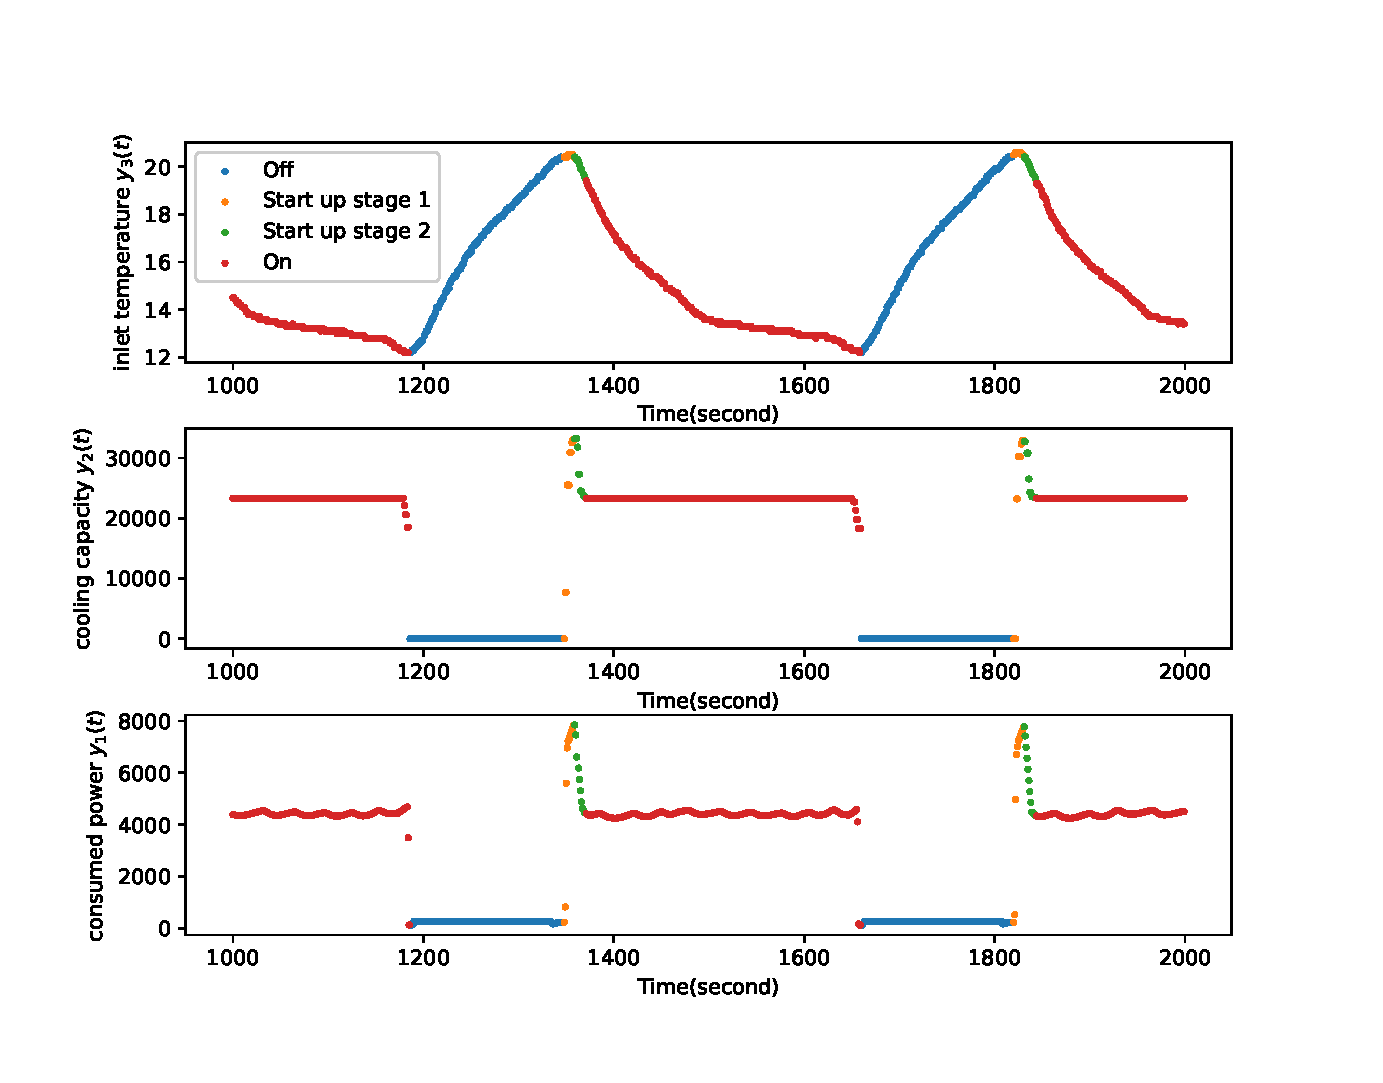
\includegraphics[width=10cm]{figures/chapter4/mark.eps}
%     \caption{Auto Stage labeling result demonstration
%     }
%     \label{fig:stages_mark}
% \end{figure}

% \subsubsection{Multi-stage transformation and duration time prediction}
% According to the prior knowledge, the property of periodic multiple-stage in the system is apparent and we can identify the transform boundaries between adjacent stages from dataset readily.

% The inputs indices include consumed power of the date center $x_1(t)$, room temperature $x_2(t)$. Two inputs variables affect the behaviors of the cooling system and determine three system outputs variables including: instant cooling power $y_1(t)$, cooling production $y_2(t)$, and inlet temperature of cooling system $y_3(t)$.
% Generally, inlet temperature $y_3(t)$ is oscillated periodically in a deterministic range defined by max setpoint $Ti_{max}$ and min setpoint $Ti_{min}$.


% \subsection{Case study 1: Operating Variables Simulation}

\subsection{模型训练}
% \subsection{Model training}
\label{sec:model_training}

本节从Seduce平台采集了四组数据集用于模型的训练与评价,四组数据集均采集于生产运行稳定时段,且运行功率有较大差异,分别为1.7kw,3.8kw,4.2kw,6.3kw。运行功率$x_1(t)$越大,说明当前热负载越高。表\ref{tab:sys_in_out_prior}中汇总了各个数据集的描述、输入输出介绍以及序列长度。在图\ref{fig:state}中,本节统计了不同热负载下,每次\textit{On}阶段和\textit{Off}阶段持续时间的分布情况。
结果表明,阶段持续时间与热负载功率值有较强相关性。在特定的热负载下,阶段持续时间${\tau}_{i}$趋于稳定。
这一结果说明,在开环预测时,利用系统的热负载输入以及外部环境温度动态地预测各个阶段的持续时间以及实现阶段自切换是具有可行性的。
% 与服务器负载功率值有较强相关性,特定数据集下的阶段持续时间分布相对稳定。
% In 图.~\ref{fig:state}, we analyse the statistical properties of duration in each stage. 
% It demonstrates that the distribution of duration ${\tau}_{i}$ is stationary and highly depends on the nearby external inputs.
\begin{figure}
\centering
\hspace{-0.1in}
\subfigure[阶段-\textit{关闭}]{\includegraphics[width=0.45\linewidth]{figures/chapter4/state1.pdf}}\hspace{-0.05in}
\subfigure[阶段-\textit{开机}]{\includegraphics[width=0.45\linewidth]{figures/chapter4/state4.pdf}}
\caption{
% The data of the four data sets are generated at different power of the server, which are 1.7kw, 3.8kw, 4.2kw and 6.3kw respectively. Compare the duration time of system on and off   under different power.
在平均负载不同的四个数据集中,\textit{启动}阶段和\textit{关闭}阶段的持续时间分布箱线图
} %图片标题
\label{fig:state}  %图片交叉引用时的标签
\end{figure}

对于四个数据集,每个数据集中的完整序列长度约为8000-10000,采样时间点为连续非均匀的,平均采样频率约为1条/秒,序列对应的时间长度约为8000s-10000s。
每个数据集的前50\%数据用于模型训练,剩下的数据中,25\%数据用于构建验证集,25\%数据用于模型测试。

对于训练集和验证集,本节使用大小为1600s的滑动窗口对原始序列进行遍历并生成训练样本。
对于每一个训练样本,根据~\ref{sec:4_notations}节的定义,前800s为条件范围,用于编码器求解预测阶段所需的初始状态,后800s为预测范围,模型预测该范围内的系统输出。
在训练过程中,选择验证集中表现最好的模型用于最终的模型评估。
由于系统输入输出的维数较低,且得益于伴随状态法(Adjoint state),不需要存储求解ODE时的完整计算图,训练AJ-ODE-Net网络对于显存的消耗是极低的。因此本节选择了较大的批大小(batch size=4096)以加速训练。
所有数据集的训练样本被随机排序并分批输入到模型训练。训练过程使用了单块型号为NVIDIA TITAN RTX的并行计算设备(GPU),其显存为24G。
隐状态变量$\boldsymbol h(t)$的大小是20,学习率设置为0.005。

% 在测试阶段,没有像构造训练集一样对测试集中的完整序列进行分割。
在测试阶段,未按照构造训练集时采用窗口分割方法对测试集序列进行拆分。
序列的前800s被送入编码器模型以生成初始状态。解码器模块在给定800s之后的剩余序列输入下,以开环的方式预测余下部分的系统输出。预测结果与测试集中的真实输出作对比以评估模型精度。
% During training, the model which performs best in validation dataset will be chosen 
% Owing to low dimensional inputs, we choose a large batch size as 4096 to accelerate training.
% In order to improve the robustness, the training samples of all data sets are randomly ordered and concatenated together before feeding into the model.
% The training phase is executed on a single NVIDIA TITAN RTX with 24G memory.


%when cooling system is off and slower decrease of inlet temperature when cooling system is working.Together with the stages of cooling system, the consumed power of cooling system $y_1(t)$ and cooling capacity $y_2(t)$ also change periodically with the frequencies and phase positions determined by inputs $x_1(t)$ and $x_2(t)$.  


\begin{table}[ht]
    \centering
\caption{系统输入输出, 不同负载下的数据集和模型的操作}
% \caption{System Inputs-Outputs, data sets based on heat load and model options}
\label{tab:sys_in_out_prior}
\begin{tabular}{cll}
\toprule
\multicolumn{1}{c}{}                                  & 变量定义                      & 描述                                    \\ \hline
\multicolumn{1}{c|}{\multirow{2}{*}{输入}}          & \multicolumn{1}{c|}{$x_1(t)$}& 服务器的瞬时功率,  $W$            \\ \cline{2-3} 
\multicolumn{1}{c|}{}                                 & \multicolumn{1}{c|}{$x_2(t)$}& 环境温度, $^{\circ}C$          \\ \hline
\multicolumn{1}{c|}{\multirow{3}{*}{输出}}         & \multicolumn{1}{c|}{$y_1(t)$}& 制冷系统功率,  $W$                  \\ \cline{2-3} 
\multicolumn{1}{c|}{}                                 & \multicolumn{1}{c|}{$y_2(t)$} & 制冷量,  $W$                     \\ \cline{2-3} 
\multicolumn{1}{c|}{}                                 & \multicolumn{1}{c|}{$y_3(t)$}& 入气口温度,  $^{\circ}C$  \\ \hline
\multicolumn{1}{c|}{\multirow{4}{*}{数据集}} & \multicolumn{2}{l}{"1.7k":服务器稳定运行在1.7kw左右, 长度: 8853s}  \\ \cline{2-3} 
\multicolumn{1}{c|}{}                                 & \multicolumn{2}{l}{"3.8k": 服务器稳定运行在3.8kw左右, 长度: 9771s}  \\ \cline{2-3} 
\multicolumn{1}{c|}{}                                 &
\multicolumn{2}{l}{"4.2k": 服务器稳定运行在4.2kw左右, 长度: 8472s}  \\ \cline{2-3} 
\multicolumn{1}{c|}{}                                 &
\multicolumn{2}{l}{"6.3k": 服务器稳定运行在6.3kw左右, 长度: 8418s} \\ \hline
% \multicolumn{1}{c|}{}                                 &
% \multicolumn{2}{l}{Proportion of dataset for training, validation, and test 5:2:5}  \\ \hline
% Dataset split & training: validation:test = 5:2:5 \\ \hline
\end{tabular}
\end{table}

\subsection{应用研究1: 运行变量仿真}
\label{sec:case-study1}
本节使用基于AJ-ODE-Net结构的编码器-解码器框架预测制冷系统的输出。
模型的预测变量为三个:进气口温度、制冷量和制冷机功率。
其中,进气口温度是受制冷系统影响的控制目标变量,表示制冷系统排出的空气温度。制冷量代表制冷系统单位时间产生的制冷量,其直接影响制冷系统中进气口温度的变化~\cite{alonso2020estimating},在压缩机不工作时,制冷量为0。制冷系统开始工作后,制冷量会突然飙升至较高水平。
制冷机功率,表示整个制冷系统的瞬时功耗。在制冷系统工作期间功耗较高,待机期间功耗较低。
% In the first place, the framework is used to simulate the operating variables of the concerned cooling system in real time, three typical variables are selected: inlet temperature, cooling production and cooling power. Where, the first variable inlet temperature is an important thermal target of data center affected by cooling production, indicating the air temperature taken by servers. The second one is cooling production generated by compressor, which acts directly on removing heat during the cooling process~\cite{alonso2020estimating},  compressor consumes most of the electricity in the cooling system. And the third estimated variable is cooling power, indicates the instant power consumed by entire cooling system. 
% 另外,系统运行过程中混合稳定和非稳定的两种过程:当系统产生冷空气时,制冷量和系统功耗可以看作是典型的稳定过程(均值和方差相对稳定)。
% 而在此过程中,进气口温度呈指数型下降,则应视为非稳定过程(均值不断下降)。这种稳定性和非稳定性过程混合的系统在工业系统中很常见,
% 所以有必要将多个H-ODE嵌入到AJ-ODE-Nets模型中。
本节同时引入普通的ODE-Net、ODE-RNN\cite{10.5555/3454287.3454765}、CDE-Net\cite{kidger2020neural}作为本章H-ODE-Net的对比模型。对比模型也可以与本章的阶段转换预测器组合,进而具备跳变系统辨识能力。AJ-ODE-Net与其他模型的对比结果如图\ref{fig:4_models}所示。
% 为了展示H-ODE在多阶段AJ框架中应用的优势,我们对其他可以用来替代H-ODE的模块进行了评估,如嵌入单个ODE模块的结构和嵌入ODE- rnn模块的结构~,并与H-ODE进行了比较,结果如图.~\ref{fig:models}所示。
% In addition, the system operating has a mixture of stationary and non-stationary processes: when the system is producing cold air, energy is consumed stably by compressor, which can be seen as a typical stationary process (with relatively fixed mean and variance). While during this process, the inlet temperature decreases in exponential way, which should be otherwise treated as non-stationary process (the mean keeps dropping). This mixture is commonly seen in industrial systems, and worth the efforts in developing H-ODE network within AJ-ODE-Net module (refer to~\ref{sec:dfa-ode-module}).
% In order to demonstrate the advantages of applying H-ODE in multi-stage AJ framework, other options like one Neural ODE structure and ODE-RNN~\cite{10.5555/3454287.3454765} structure as substitutions for H-ODE are evaluated as well to have a comparison, the results are shown in 图.~\ref{fig:models}.
其中图~\ref{fig:4_models}(a)为真实的系统输出,图~\ref{fig:4_models}(d)为采用带有H-ODE-Net的AJ-ODE-Net模型的预测结果。
在图~\ref{fig:4_models}(b)中,将AJ-ODE-Net替换为一个单一的稳定型ODE-Net,此时各阶段的转换不受持续时间预测器控制。
% 对比(b)和(d)可以发现,使用单一ODE模型难以对各个阶段间的系统切换边界处给出准确的拟合,尤其对于持续时间较短的阶段转换位置,如阶段1与阶段2,预测效果明显差于AJ-ODE-Net。
可以发现,使用单一ODE模型时难以对各个阶段间的系统切换边界处给出准确的拟合,尤其对于持续时间较短的阶段转换位置,如阶段1与阶段2,预测效果明显较差。
在图~\ref{fig:4_models}(c)中,采用ODE-RNN~\cite{10.5555/3454287.3454765}替换了AJ-ODE-Nets中用于建模稳定和非稳定混合输出的H-ODE-Net模块。
可以发现经过替换后,网络难以平滑地预测系统输出。
相比于其他模型,图~\ref{fig:4_models}(d)中AJ-ODE-Net预测的系统输出十分精确,且在阶段转换的边界处能够极好地识别系统输出的剧烈变化。
% Where 图.~\ref{fig:models}(a) is the pattern of original data sets and 图.~\ref{fig:models}(d) is the estimation results by adopting AJ-ODE module with H-ODE-Net cells. 
% In 图.~\ref{fig:models}(b), the AJ-ODEs module is replaced by one stationary neural-ODE, in this case, transition of stage is not governed by duration predictor, which could have troubles in precisely fitting dynamics of each stage, especially for the short stage transitions. In 图.~\ref{fig:models}(c) the hybrid stationary and non-stationary 
% H-ODE cells in AJ-ODE-Nets are replaced by another widely used structure ODE-RNN~\cite{10.5555/3454287.3454765}, which can hardly simulate smooth physical process. 
\begin{figure*}
\centering
\hspace{-0.2in}
\subfigure[原始数据]{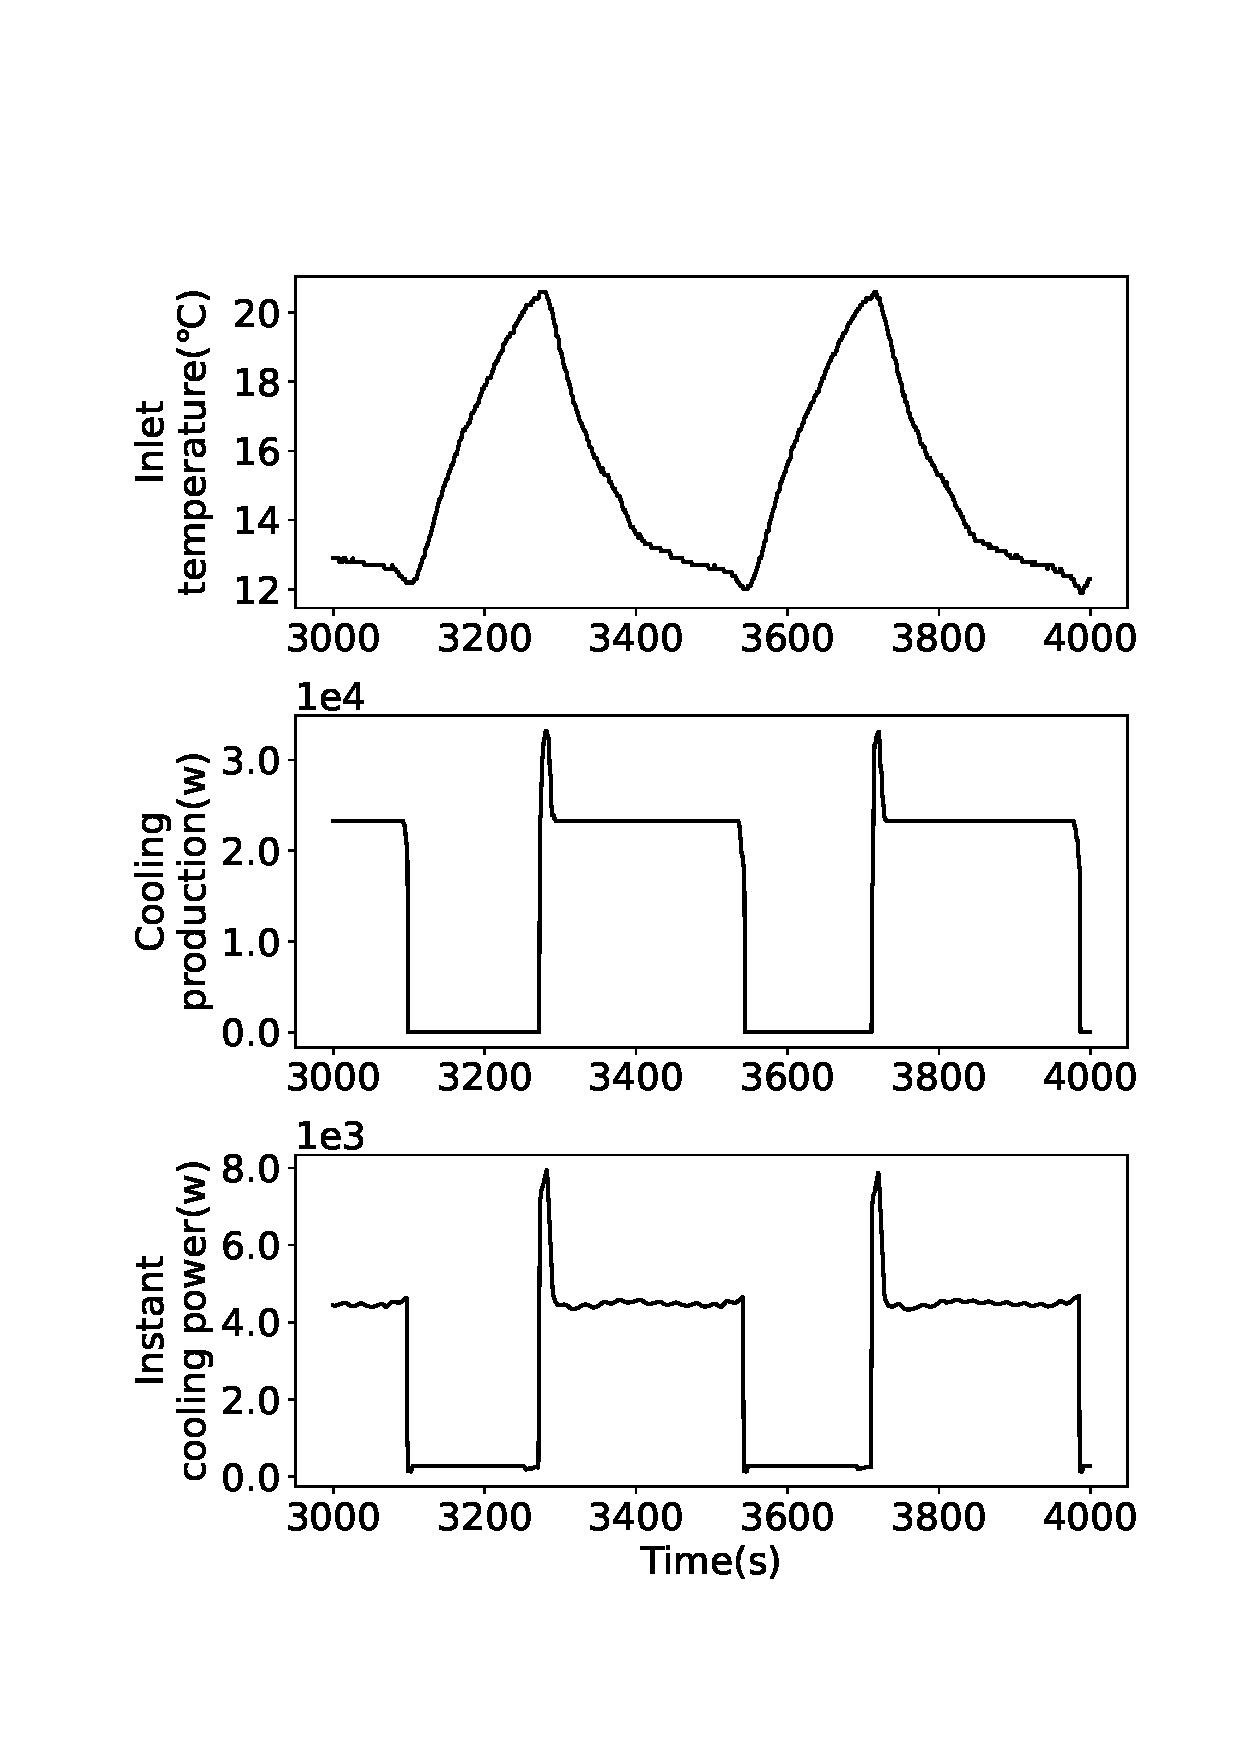
\includegraphics[width=0.45\linewidth]{figures/chapter4/truth.pdf}}\hspace{-0.08in}
\subfigure[单ODE网络]{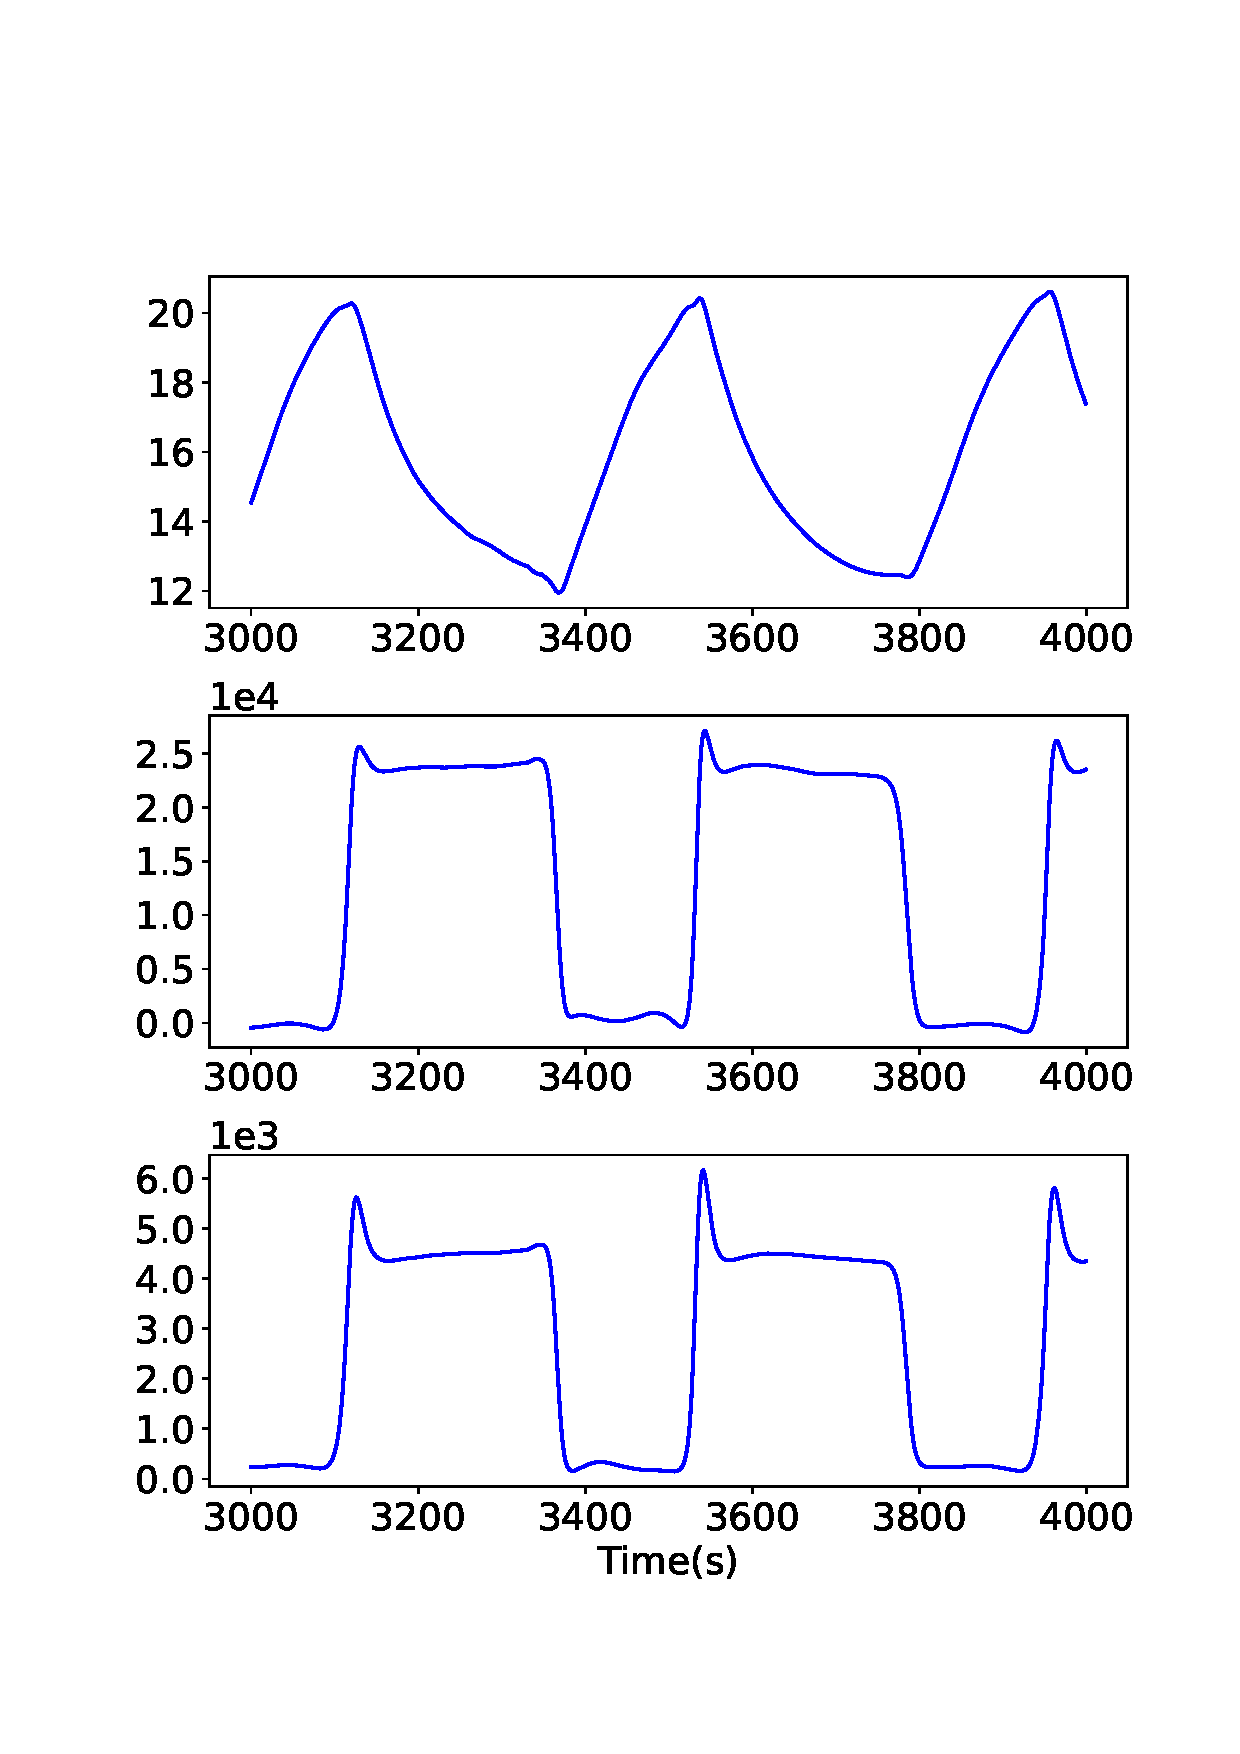
\includegraphics[width=0.45\linewidth]{figures/chapter4/one.pdf}}\hspace{-0.08in}
\subfigure[自跳跃结构+ODE-RNN]{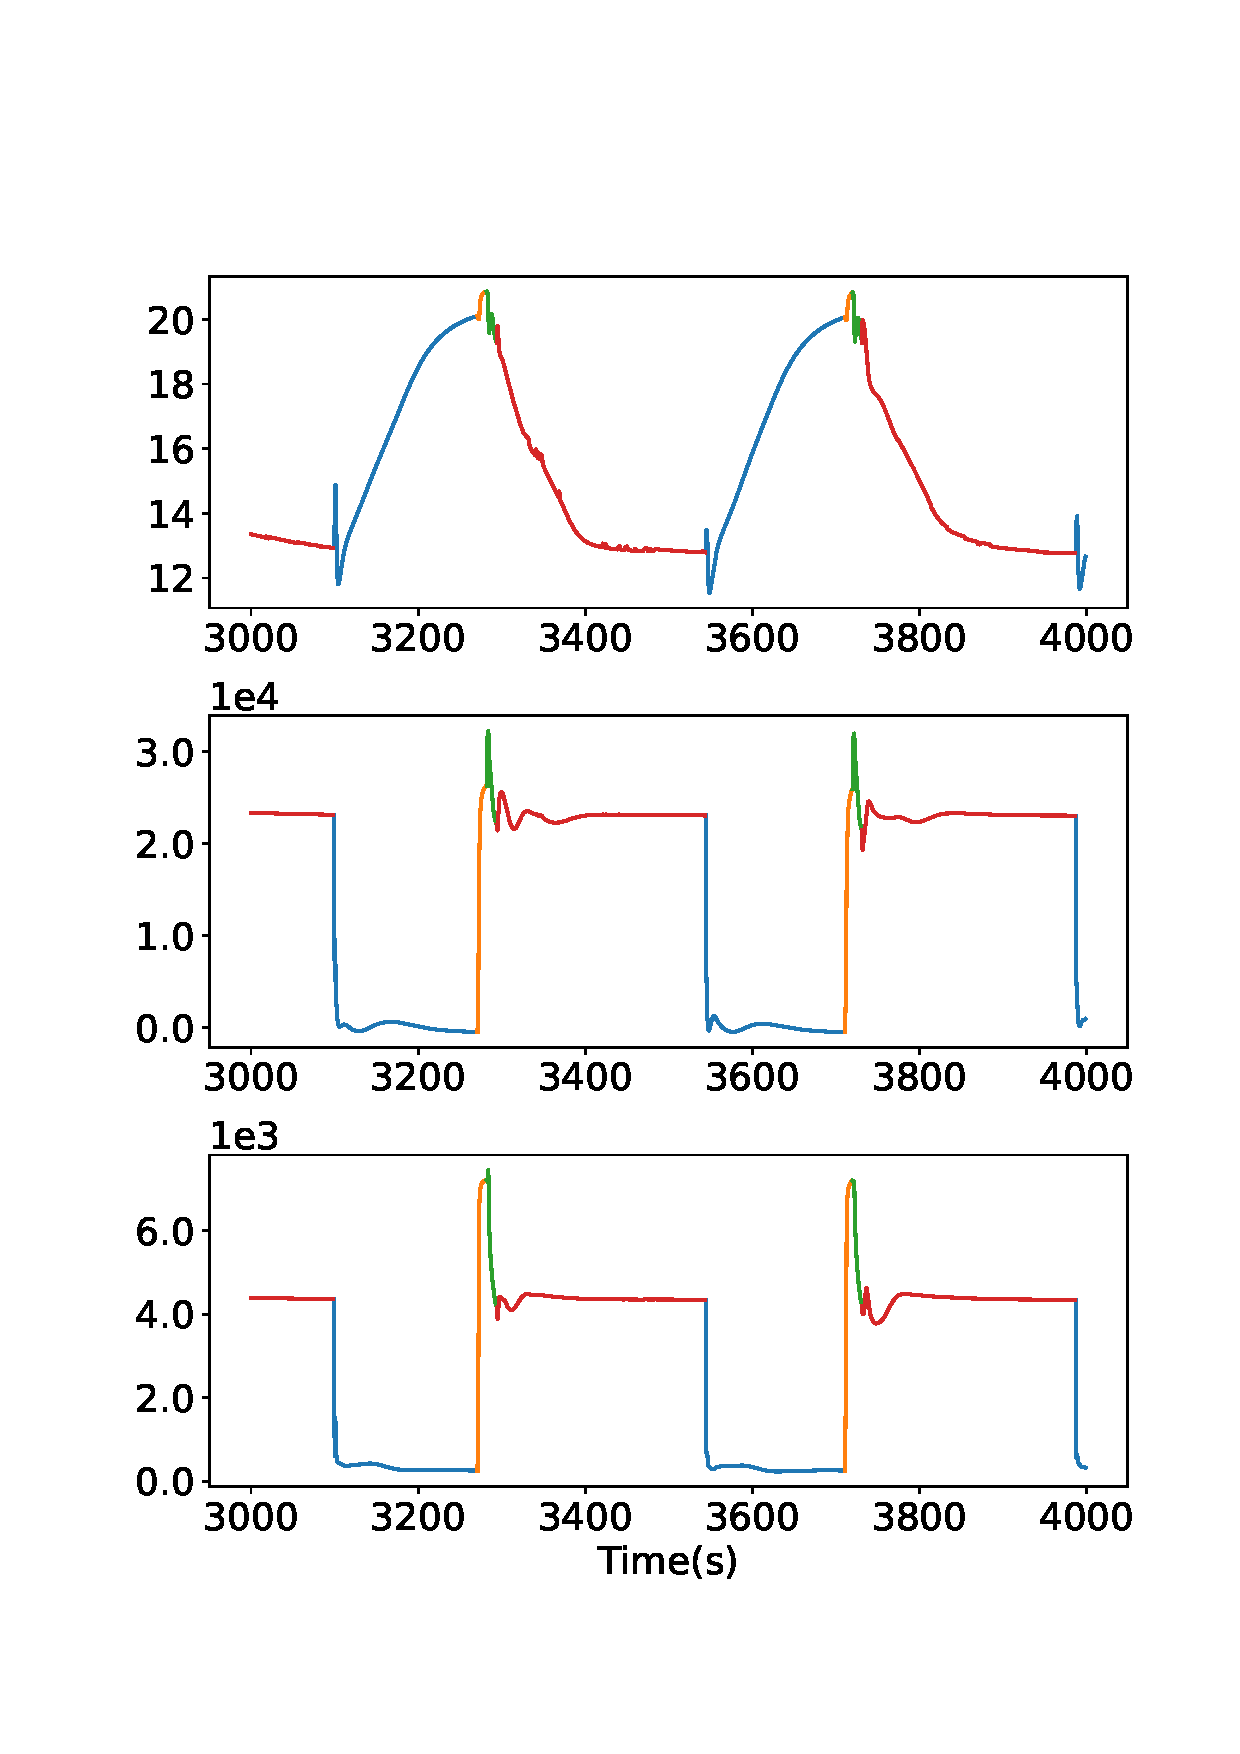
\includegraphics[width=0.45\linewidth]{figures/chapter4/rnn.pdf}}\hspace{-0.08in}
\subfigure[自跳跃结构+H-ODE-Net(本文方法)]{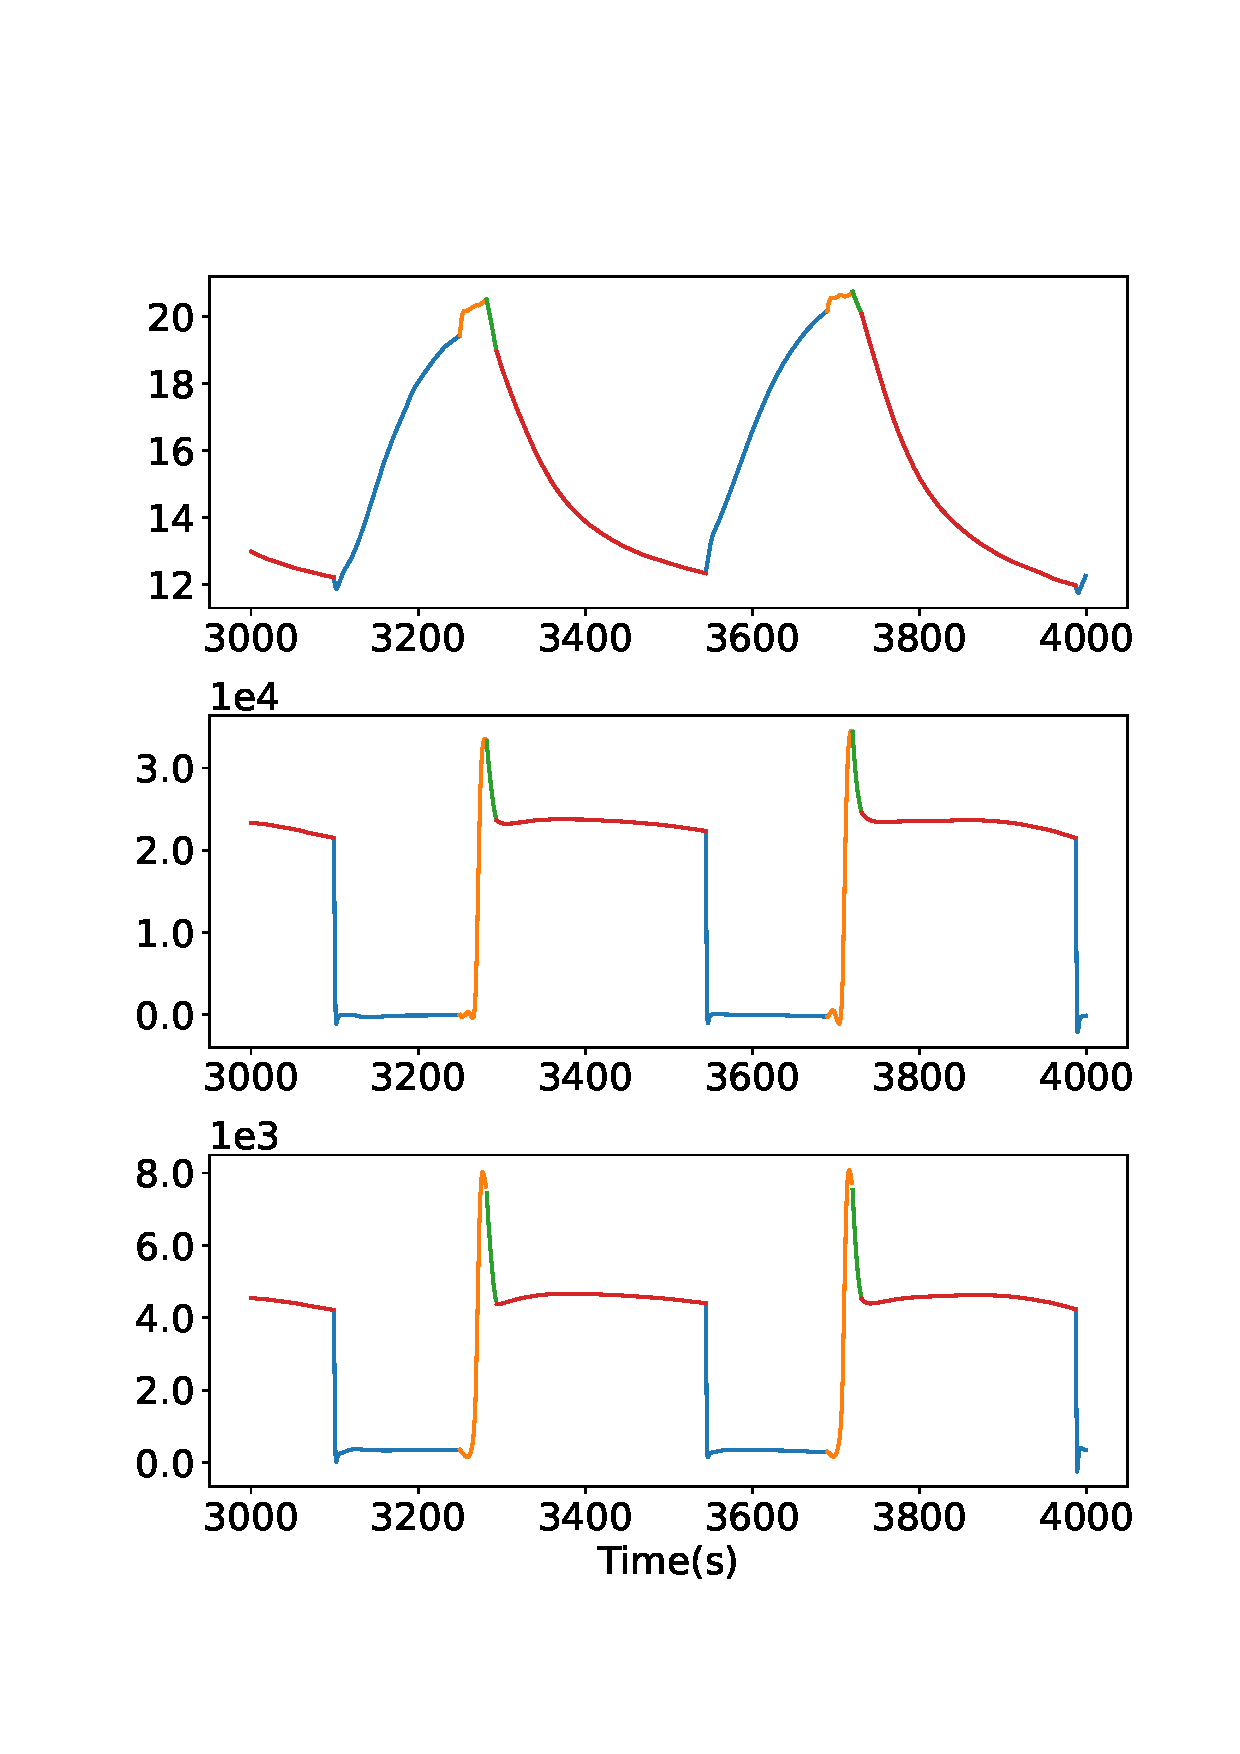
\includegraphics[width=0.45\linewidth]{figures/chapter4/ours.pdf}}
\caption{不同模型预测进气口温度、制冷量、制冷机功率的效果对比} %图片标题
\label{fig:4_models}  %图片交叉引用时的标签
\end{figure*}
% 图.~\ref{fig:}
% \centering
% \hspace{-0.1in}
% \begin{figure}
%     \centering
%     \hspace{-0.1in}
%     \subfigure[The time of state-off]{\includegraphics[width=4.7cm]{figures/chapter4/3.8k.png}}\hspace{-0.2in}
%     \subfigure[6.3k]{\includegraphics[width=4.7cm]{figures/chapter4/6.3k.png}}
%     \includegraphics[width=10cm]{figures/chapter4/3.8k.png}
%     \caption{Prediction results of 3.8k-power}
%     \label{fig:3.8k-power}
% \end{figure}
% \begin{figure}
%     \centering
%     \includegraphics[width=10cm]{figures/chapter4/6.3k.png}
%     \caption{Prediction results of 6.3k-power}
%     \label{fig:6.3k-power}
% \end{figure}
上述实验表明,使用多阶段模型能够将先验知识集成到模型中,相比于单模型结构,能够更好地预测多阶段系统的阶段转换边界。
同时,结合了非稳定输出和稳定输出的H-ODE-Net模型能够有效地对系统的多个输出项进行学习,相比于忽视了系统输出时序特性的ODE-RNN模型,能够更准确地预测系统的输出。

% In addition to the predicted accuracy, in using AJ method, the prior knowledge can be integrated into models, to enable advanced studies like the simulation of configuration adjustments, dynamical control and energy consumption optimization. Conversely, for one Neural-ODE or AJ-ODE-RNN structures, it is not applicable.
接下来,本小节将定量地评估不同模型的预测精度。由于本文关注于开环预测问题并且需要模型自发地进行阶段切换。伴随着预测范围长度的增加,对于相位的估计误差也将不断累积。
当预测结果中各阶段开始、结束的位置与系统真实输出中阶段的起止位置无法对齐时,此时点对点的误差评估并不适用于量化评估模型的预测误差。
因此,本节对模型预测功耗的长期累积结果进行评估。
对于不同功率的数据集,采用训练过的模型预测制冷系统在未来预测范围$[{t_I:t_{I+L}}]$(共120分钟)下的功耗。
% In terms of the estimation accuracy, given that AJ-ODE-Nets is applied for open loop estimation and govern the stage transition automatically, the running phases could be affected significantly by the initial point and accumulative error, therefore the point to point accuracy is less meaningful. 
% Accordingly, in order to evaluate the long term simulation capability of the framework, the accumulative energy consumption is estimated over different predictive length, from five minutes to two hours. 
% For the datasets with different power, we employ the trained model to predict the future energy consumption with the predictive range $[{t_I:t_{I+L}}]$ equaling 120 minutes.
% The length of the predicted range ${t_I:t_{I+L}}$ is 120 minutes.
% The predictive error of the accumulative power consumption is evaluated sectionally and measured as Mean Absolute Percentage Error (MAPE).
% By defining the size of the evaluation window as $T$, the prediction error of consumed power, $E(T)$, is measured as:
在序列预测结果基础上,按时间尺度对瞬时功耗进行积分以得到某一时间长度(T)下的累积功耗预测值。
进一步地,可以定义预测功耗的平均绝对百分比误差,$\text{MAPE}(T)$:
% The Mean Absolute Percentage Error (MAPE) of the predicted energy consumption, $\text{MAPE}(T)$, is defined based on the size of the evaluation window $T$:
% \vspace{-5pt}
\begin{equation}
\text{MAPE}(T) = \frac{100\%}{n}\sum\limits_{i=1}^{\lfloor\frac{t_{I+L}-t_I}{T}\rfloor}\text{APE}(t_I+T*(i-1),t_I+T*i)
\label{equ:energy_mape}
\end{equation}
其中,其中绝对百分比误差(APE)定义如下:
\begin{equation}
\text{APE}(t_1,t_2) = \left|\frac{\int_{t_1}^{t_2}\hat{y}_1(t)dt-\int_{t_1}^{t_2}y_1(t)dt}{\int_{t_1}^{t_2}y_1(t)dt}\right|
\end{equation}
其中,绝对百分比误差$\text{APE}(t_1,t_2)$衡量了时间范围$[t_1, t_2]$内预测功耗和真实功耗之间的相对误差。
图\ref{fig:mape_evolution}描述了评估窗口的大小T对于评估结果$MAPE(T)$的影响。
可以看出,随着$T$的增加,$\text{MAPE}(T)$ 在开始时剧烈下降,然后缓慢下降。
当评窗口大小超过35分钟时,所有数据集的MAPE都趋于稳定,说明此时真实输出序列与预测序列之间的阶段起止位置相位差对于评估长期功耗的预测精度不再产生影响。
因次本节对比了$T=30$分钟下,不同模型对于累积功耗预测结果的MAPE,结果如表~\ref{tab:Compare power}所示。
对于所有数据集,AJ-ODE-Net预测结果的MAPE稳定低于5\%,优于其他三个对比模型。
充分证明了本文提出的AJ-ODE-Net模型及编码器解码器框架能够以开环预测的方式在长时间尺度下精确地仿真制冷系统的累积功耗。

从计算复杂性的角度,本节对四个模型在测试集单批数据上执行式\eqref{equa:initial_state}以及式\eqref{equ:decoding}两个过程的时间消耗进行了对比。
普通ODE-Net作为耗时最短的模型,将其时间消耗作为基准,其他模型的推理时间均除以该基准以得到相对尺度下的耗时指标。
相应地,普通ODE-Net的相对时间消耗为1.0。对比结果如表\ref{tab:Compare power}的最后一列所示。
相对时间尺度下的对比结果表明引入阶段转换预测器会增加计算开销,该时间消耗主要用于更新阶段变量及阶段持续时间。

% % The Mean Absolute Percentage Error (MAPE, see 式~\ref{equa:mape}) has been calculated between real and estimated energy consumption in the test datasets. We select a series with a time duration of 120min, In order to calculate the power consumption of different duration $t_r$, from 5 minututes to 120 minututes.According to the formula $ n=120/tr$, get n sample points. 
% % Where, $n$ is the number of sample points, $\hat{e}_i$ is the estimated value and $e_i$ is the real value.  
% % As illustrated by 式~\ref{equa:energy},  where the value $a$ is the beginning of this sequence time, the value $b$ is the ending, and $y_1(t)$ is the instantaneous consumed power of the cooling  system. 
% % The energy consumption is calculated through the integral of power over a period of time. 
% where absolute percentage error(APE) measures the relative error of the estimated energy consumption, which is calculated through the integral of power over a period of time $[t_1, t_2]$. 
% 图.~\ref{fig:mape_evolution} describes how does the size of evaluation window affect the evaluated results $E(T)$.
% % The 图.~\ref{fig:mape_evolution} shows the MAPE of the energy consumption estimation results over prediction duration. 
% It can be seen that, with the increase of $T$, $\text{MAPE}(T)$ declines dramatically at the beginning then becomes smaller and smaller. 
% When the size of evaluation window exceeds 35 minutes, the MAPE of all datasets are stably below 5\%, the phase difference will have little impact on estimating long-term energy consumption. 
% Tab.~\ref{tab:Compare power} also compares the MAPE of predicted energy consumption from proposed AJ-ODE-Net with the results from the other competitors.
% The results indicate that, in terms of the open loop estimation, the proposed framework can eliminate the impact of initial point and obtain satisfying accuracy for energy consumption simulation with a predictive range longer than half an hour. 
\begin{table}[t]
    \centering
    % \caption{
    % of H-ODE-Net and 
    % Power estimation error comparison between One-ODE and H-ODE ,The total length of each test set is 120 minutes. Select the sequence every 30 minutes, calculate the power consumption of the truth value and the predicted value, and then calculate the MAPE. Truth power consumption$P_{truth}=(p_1,p_2,p_3,p_4)$,Predicted power consumption$P_{pred}=(\hat{p_1},\hat{p_2},\hat{p_3},\hat{p_4})$
    % The comparison of energy consumption prediction and the relative computational efficiency}
    \caption{不同模型累积能耗预测精度和推理时间的对比}
    % \resizebox{0.9\linewidth}{!}{
    \begin{tabular}{lccccc} 
    \toprule
                                & \multicolumn{4}{c}{\textbf{\textbf{热负载}}} & \multirow{2}{*}{\begin{tabular}[c]{@{}c@{}}相对 \\时间\end{tabular}}  \\
    \multicolumn{1}{c}{}        & 1.7k          & 3.8k          & 4.2k          & 6.3k               &                                                                           \\ 
    \hline
    \textbf{AJ-ODE-Net}(本文模型) & \textbf{4.20} & \textbf{1.51} & \textbf{3.46} & \textbf{2.53}      & 3.2                                                                        \\
    单个ODE-Net              & 6.18          & 19.99         & 6.24          & 3.39               & 1.0                                                                         \\
    自跳跃结构+受控微分方程网络\cite{kidger2020neural}     & 8.25         & 2.73          & 6.62         & 3.87              & 3.8                                                                        \\
    自跳跃结构+ODE-RNN & 38.26         & 9.94          & 10.58         & 31.90              & 3.4                                                                        \\
    \bottomrule
    \end{tabular}
    % }
    \label{tab:Compare power}
    % \vspace{-15pt}
    \end{table}

% \begin{equation}
% \label{equa:mape}
%     MAPE=\frac{100\%}{n}\sum\limits_{i=1}^{n}|\frac{\hat{e_i}-{e_i}}{e_i}|
% \end{equation}


% \begin{equation}
% \label{equa:energy}
%     Energy = \int_{a}^{b}y_1(t)dt
% \end{equation}

% \begin{equation}
% \label{equa:energy}
%     n = 2/x
% \end{equation}

\begin{figure}
    \centering
    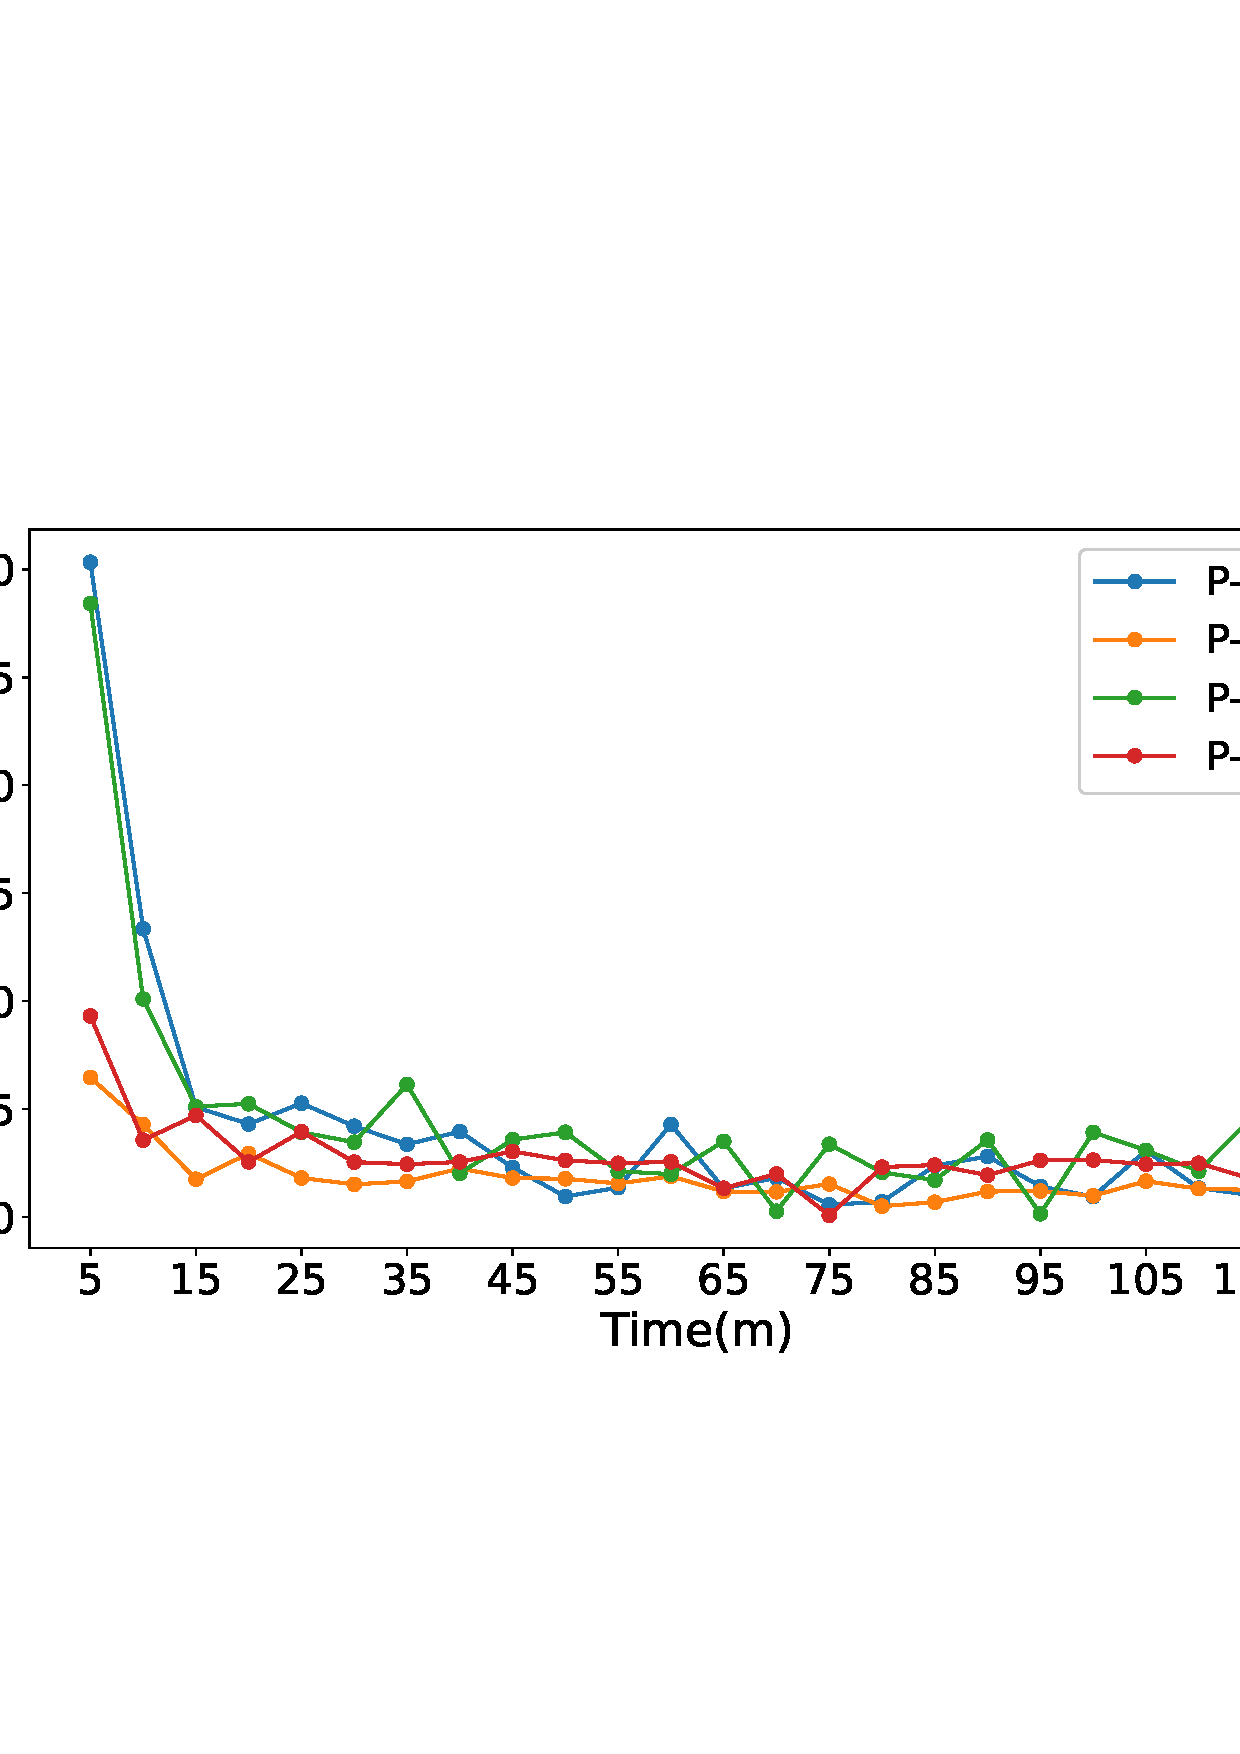
\includegraphics[width=0.8\linewidth]{figures/chapter4/power_error.pdf}
    \caption{预测不同时间长度的功耗的MAPE的变化}
    \label{fig:mape_evolution}
\end{figure}

%Relative error of predicted power consumption at different intervals,According to the instant cooling power sequence value predicted by AJ-ODE-Nets, calculate the power consumption of the system over a period of time, compare it with the real power consumption value, and calculate the error.  Compare the power consumption error between the real value and the predicted value for different duration time (5min, 10min... 120min)


%Compare the prediction effects of different models. 图.re a is the truth sequential data, figure B is the prediction result of one stable ODE model, figure C is the experimental effect of Ode RNN, and figure D is the result of our model

\subsection{应用研究2: 制冷系统进气口温度设定点优化}
\label{sub:case-study2}
进气口温度上下限设定值(上限$Ti_{\max}$和下限$Ti_{\min}$)是影响制冷系统运行、保证运行环境安全的关键设置参数。
% 通常,系统要设定通入进气口的空气温度阈值,以保证运行环境的安全。
% 通常,对于大部分的制冷系统,初始的进气口温度设定点是固定的,配置值低于ASHRAE TC9.9~\cite{ashraeTC992011}(数据中心电源设备热指南和最佳实践)中定义的标准,没有充分考虑实际的制冷需求。
对于本章研究的制冷系统,其默认温度阈值为$12^\circ C$,$20^\circ C$。
从数据集可以观察到进气温度在上下阈值之间周期性变化。
由于默认温度设置未充分考虑实际的制冷需求,会存在一定程度的能源浪费。
出于提高能源效率以及确保生产过程安全的目的,本节在保持温度上阈值不变的情况下,通过优化下阈值以减少制冷消耗。
然而,想要精确地找到最佳温度阈值是困难的。
如果阈值设置太低,由于过度制冷会浪费大量电能。
如果阈值设置太高,压缩机的制冷重启过程将更加频繁。
从图~\ref{fig:4_models}中可以看出,制冷系统重新启动时的功耗显著高于提供稳定制冷时的功耗。
因此,盲目地增加温度下阈值反而可能会导致整体能耗的增加。
% 实际上,最佳温度设定点随热负载的不同而变化,尤其是温度下限。如果下限设置过低,会因过度制冷过多而浪费电能;过高会导致压缩机频繁停机和启动,如图1所示(见表~\ref{tab:cooling_dfa}),在阶段一启动时功率峰值会很高,这些峰值过多会浪费额外的电能,。

本节试图寻找最优温度下限以期望达到最佳的能源效率。形式化地,寻找最优温度下限$Ti_{\min}^{*}$可以表示为一单目标优化问题,问题中需要考虑的因素包括:热负载、环境温度、进气口温度的上下限:
\begin{equation}
    \begin{aligned}
       Ti^*_{\min}&=\mathop{\arg\min}\limits_{Ti_{\min}} \int_{0}^{T} \hat{y}_{1}(t) dt \\
       &\text{s.t. } \hat{\boldsymbol{Y}}_{0: T}=F\left(\boldsymbol{X}_{0: T},Ti_{\min}, Ti_{\max},\boldsymbol{\zeta}\right),
       Ti^*_{\min}\leq \hat{y}_{3}(t) \leq Ti^*_{\max}
    %    &\text{s.t. }\begin{aligned}
    %    \end{aligned}
    %    \text{s.t. } \hat{\boldsymbol{Y}}_{0: T}=F\left(\boldsymbol{X}_{0: T},Ti_{\min}, Ti_{\max},\boldsymbol{\zeta}\right)
    %    &\text{s.t. } \hat{\boldsymbol{Y}}_{0: T}=F\left(\boldsymbol{X}_{0: T},Ti_{\min}, Ti_{\max},\boldsymbol{\zeta}\right)
    \end{aligned}
    \label{equ:optimazition}
    \end{equation}
其中$\hat{\boldsymbol{Y}}_{0: T}$和$\hat{y}_{1}(t)$分别表示模型预测的系统输出以及预测出的瞬时功耗。
在给定系统输入和恒定上限值的条件下,被优化变量为温度下阈值,优化目标是最小化累计能耗。
式\eqref{equ:optimazition}中的$\boldsymbol{X}_{0: T}$为测试数据集中的系统输入,其中包括所有时刻的热负载以及环境温度。
$F(\cdot)$表示在给定输入和温度阈值$Ti_{\max}$和$Ti_{\min}$下,预测制冷系统的输出。
% The inlet temperature set points are one of the key configurations of cooling systems. Generally, they put the temperature variation thresholds (upper and lower boundaries) for the air temperature to the front of the servers, to guarantee the ambient and secure operating environment. 
% Normally, for the workplace like Data Centers, the initial set points are fixed and configured far below the standards defined by ASHRAE TC9.9~\cite{ashraeTC992011} (Data Center Power Equipment Thermal Guidelines and Best Practices), without considering the actual cooling requirement. 
% Actually, optimal temperature set points vary with the heat load, especially for the lower boundary: if it is set too low, energy will be wasted due to over cooling; if too high, compressor may suffer from frequent stop and restart, additional energy can be wasted due to too many power peak as seen in stage 1 (refers to Tab.~\ref{tab:cooling_dfa}). 

本节利用上一节~\ref{sec:case-study1}中训练的编码器-解码器AJ-ODE-Net模型,
在给定不同下阈值温度设定点的情况下,仿真制冷系统能耗以及进气温度变化,同时统计120分钟内的累积制冷能耗。
实验采用\secref{sec:case-study1}中热负载分别为1.7k、3.8k和6.3k的三个数据集。
温度下阈值设置点从$12^{\circ}C$逐渐增加到$18^{\circ}C$,调整间隔为$0.5^{\circ}C$ 。
% In order to simulate the cooling system with different $Ti_{\min}$, the prediction in $F(\cdot)$ is slightly different from the trained model $f(\cdot)$.

为了模拟不同$Ti_{\min}$下冷却系统的运行过程,$F(\cdot)$中的预测过程与式\ref{equa:problematique}的原始训练模型$f(\cdot)$略有不同。
% In particular, the sojourn time predictor in stage \textit{On} is replaced by a specific transformation rule.
在阶段\textit{On}下的持续时间预测器被特定的转换规则所替代。
% Just as the rule in Table~\ref{tab:cooling_dfa}), the stage immediately transitions from 3 (\textit{On}) to 0 (\textit{Off}) if the inlet temperature is cooled down to $Ti_{\min}$. 
如表~\ref{tab:cooling_dfa}所示规则,当进气口温度经过冷却下降到$Ti_{\min}$,预测模型立即将阶段变量从3(\textit{On})过渡到0(\textit{Off})。
    % The stage transition predictor in the proposed model is designed based on sojourn time prediction,  nevertheless, the rules could also be set manually in order to meet simulation requests.
尽管AJ-ODE-Net中的阶段转换预测器是基于持续时间预测器设计的,为了满足不同制冷运行参数仿真的需要,模型支持将持续时间预测器替换为其他的状态转换规则。
虽然在上述模拟过程中的温度下限与训练数据集对应的阈值参数是不同的,但AJ-ODE-Net允许手动调整阶段过渡阈值以支持外推预测。
    % Although the lower temperature threshold in simulations is out of the range of the training dataset, AJ-ODE-Net can still support extrapolation by adjusting manually stage transition thresholds.
相比于没有引入系统先验的稳态模型~\cite{Yilmaz2007},基于先验知识设计的模型具有更好的可扩展性,更便于实现灵活的系统仿真。
    % Compared with the steady state model~\cite{Yilmaz2007}, the prior knowledge-informed model is more interpretable and extensible.
    % Meanwhile, in order to model the variation of inlet temperature as a non-stationary process, the temperature is made to climb steadily during stage \textit{Off} and decreased steadily during stage \textit{On}.
同时,本章将进气口温度的变化建模成非平稳过程,使得在阶段\textit{Off}期间,进气温度将会稳定地上升,在阶段\textit{On}期间,温度会稳定地下降。
% 这两个性质能够确保进气温度必然能够触达给定的阈值。
    % This property is consistent with the prior knowledge of the system and is necessary to guarantee that the inlet temperature will continue to vary until reach the wanted thresholds.
这一特性与系统的先验知识一致,是保证进气口温度能够持续变化直至达到阈值的必要条件,有效避免了模型无限期停留某一阶段内难以跳出的情况。

% 在下边界温度设定点不同的情况进行系统仿真实验中,我们对于从\textit{On}阶段到\textit{Off}阶段的转换过程,用了一个转换规则替换了持续时间预测器。
% 如表~\ref{tab:cooling_dfa}所示的系统先验知识,随着制冷系统温度降低,当前进气口温度小于$Ti_{min}$时,系统将切换到阶段 \textit{Off},
图~\ref{fig:lowerbound_simulation}展示了对于热负载约为3.8k的数据集,设置不同进气温度下限时,制冷系统在1000秒内的瞬时功率变化情况。
% 对制冷系统的影响。
% 仿真时间为1000秒。
随着温度下限设定点从$12^{\circ}C$增加到$18^{\circ}C$,在相同的持续时间内,系统处于稳定制冷阶段的时间不断缩减。与此同时,1000秒内包含了更多的制冷系统启停周期。这导致系统的主要功耗来自于由\textit{Off}阶段转变为\textit{on}阶段的系统启动功耗,而非制冷功耗。

% In order to find the optimal lower boundary temperature set points under different heat loads. 
% we make use of the Encoder-Decoder AJ-ODE-Net model built in the first case study~\ref{sec:case-study1}, and run simulations by calculating the energy consumption within same duration under different lower temperature set point for three datasets.
% % as they represent for different heat loads (higher IT loads will generate more heat). 
% The three datasets represent for different average heat loads (higher IT loads will generate more heat) including 1.7k, 3.8k, and 6.3k.
% In each simulation with specific lower boundary temperature $Ti_{min}$, we substituted the duration predictor with a rule in the transformation from \textit{On} stage to \textit{Off} stage.
% With the cooling system brings the temperature down, the system will switch to the stage \textit{Off} when the current inlet temperature is smaller than $Ti_{min}$, as like the system prior knowledge shown in Tab.~\ref{tab:cooling_dfa}.
% % The set points can be modified in Stage Transition Predictor (refers to Sec.~\ref{sec:stage_trans_predic}), where the configurations are integrated as system prior knowledge. 
% 图.~\ref{fig:lowerbound_simulation} illustrates the impact of different lower boundaries on the behaviors of cooling system (dataset 3.8k), with the set point increasing from $12^{\circ}C$ to $18^{\circ}C$, more loops are included within same duration.
% The main stages which consume the energy most change from \textit{On} stage to \textit{start up 1} and \textit{start up 2} stage.
\begin{figure*}[h]
\centering
\subfigure[$12^{\circ}C$]{\includegraphics[width=0.45\linewidth]{figures/chapter4/12.pdf}} \hspace{-0.1in}
\subfigure[$14^{\circ}C$]{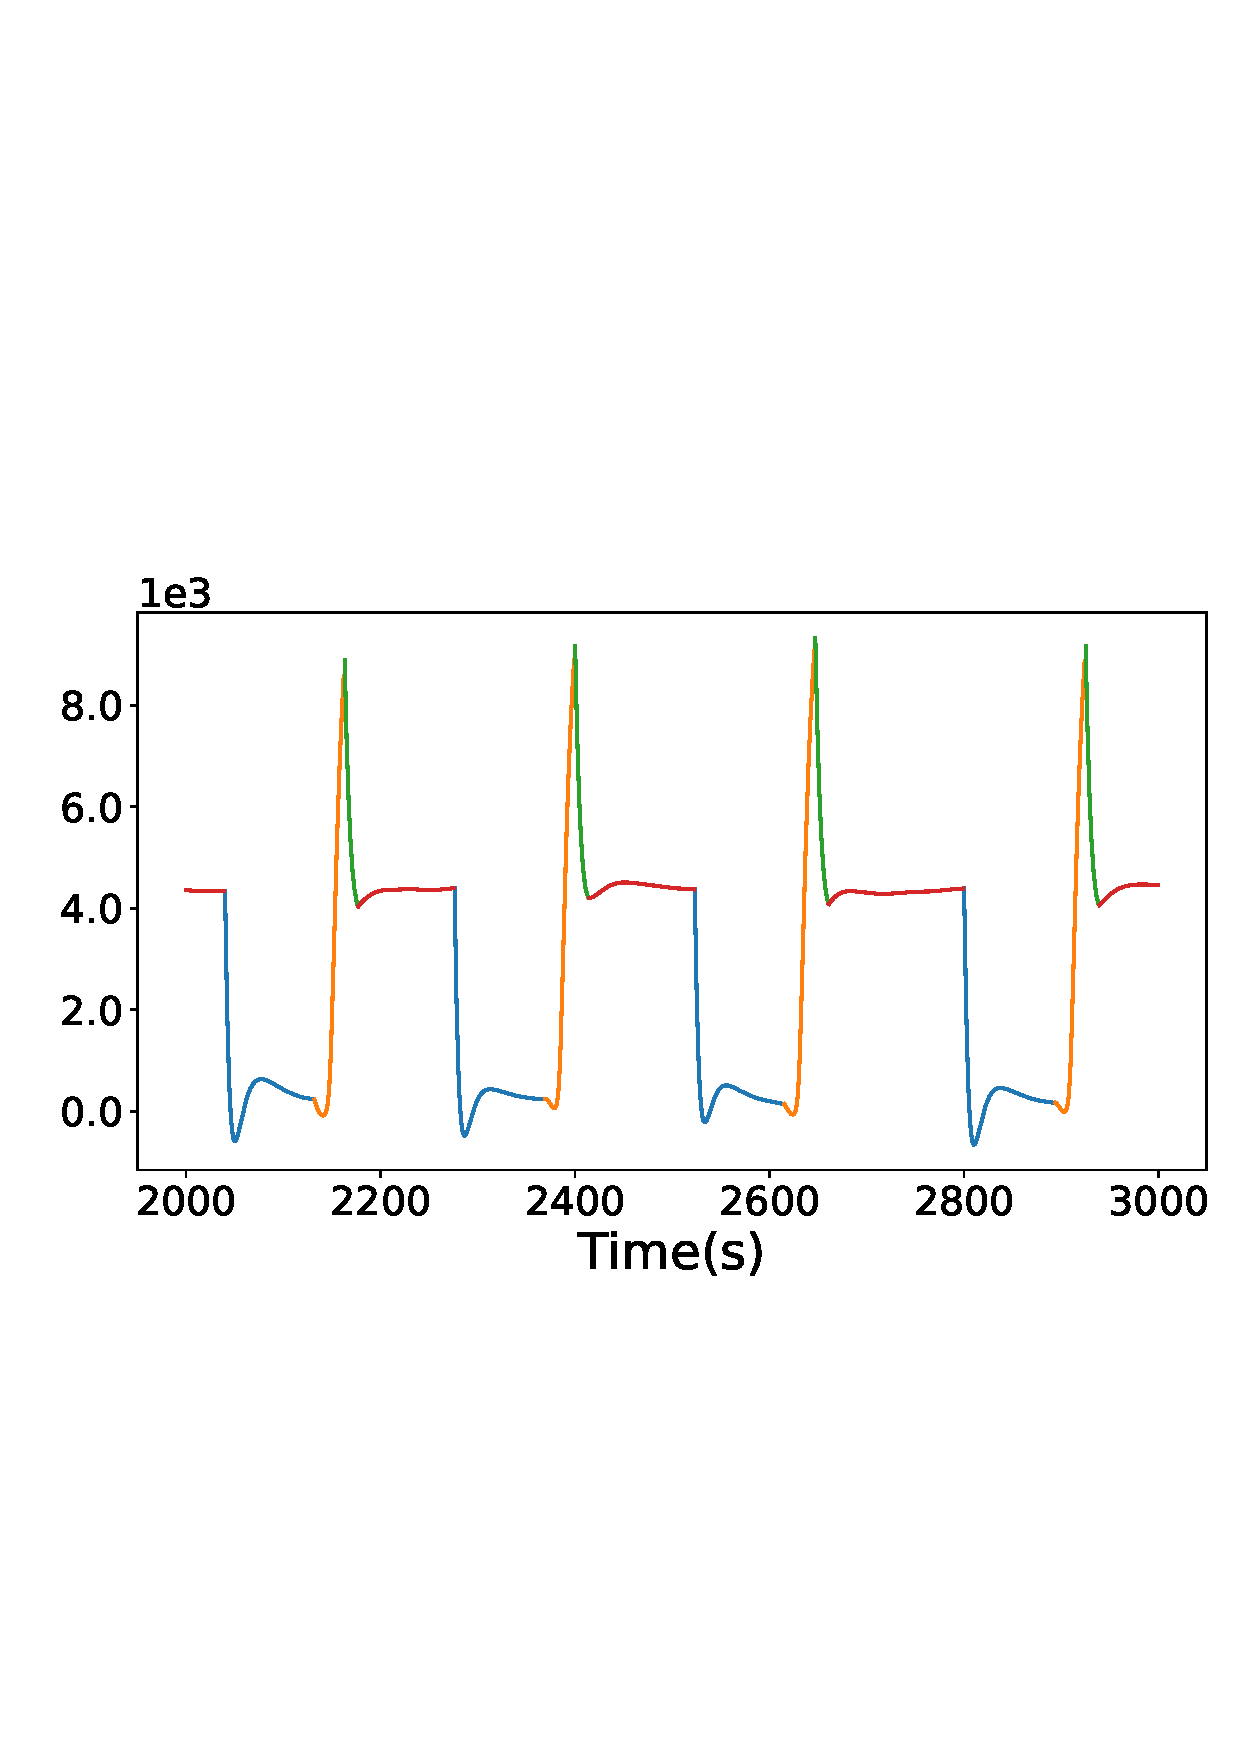
\includegraphics[width=0.45\linewidth]{figures/chapter4/14.pdf}} \hspace{-0.1in}\\
\subfigure[$16^{\circ}C$]{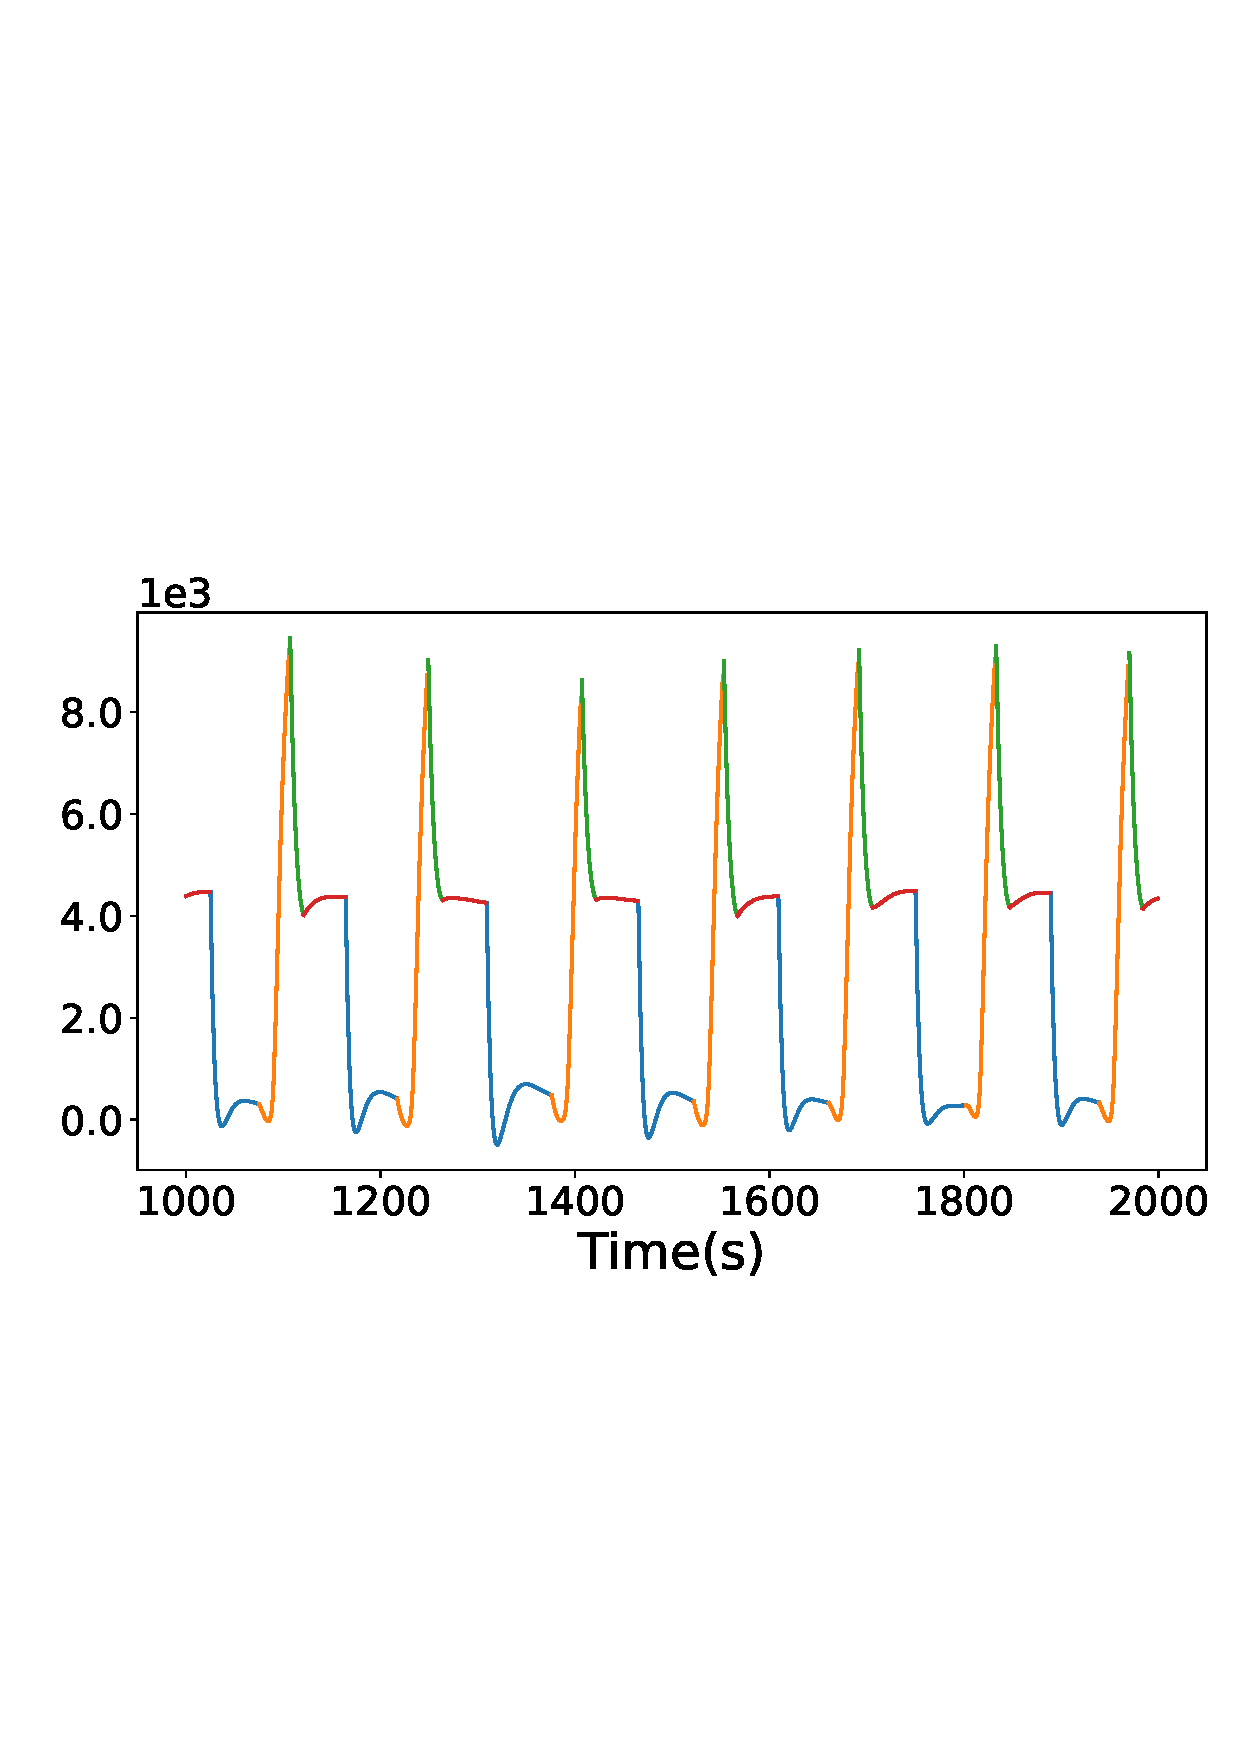
\includegraphics[width=0.45\linewidth]{figures/chapter4/16.pdf}} \hspace{-0.1in}
\subfigure[$18^{\circ}C$]{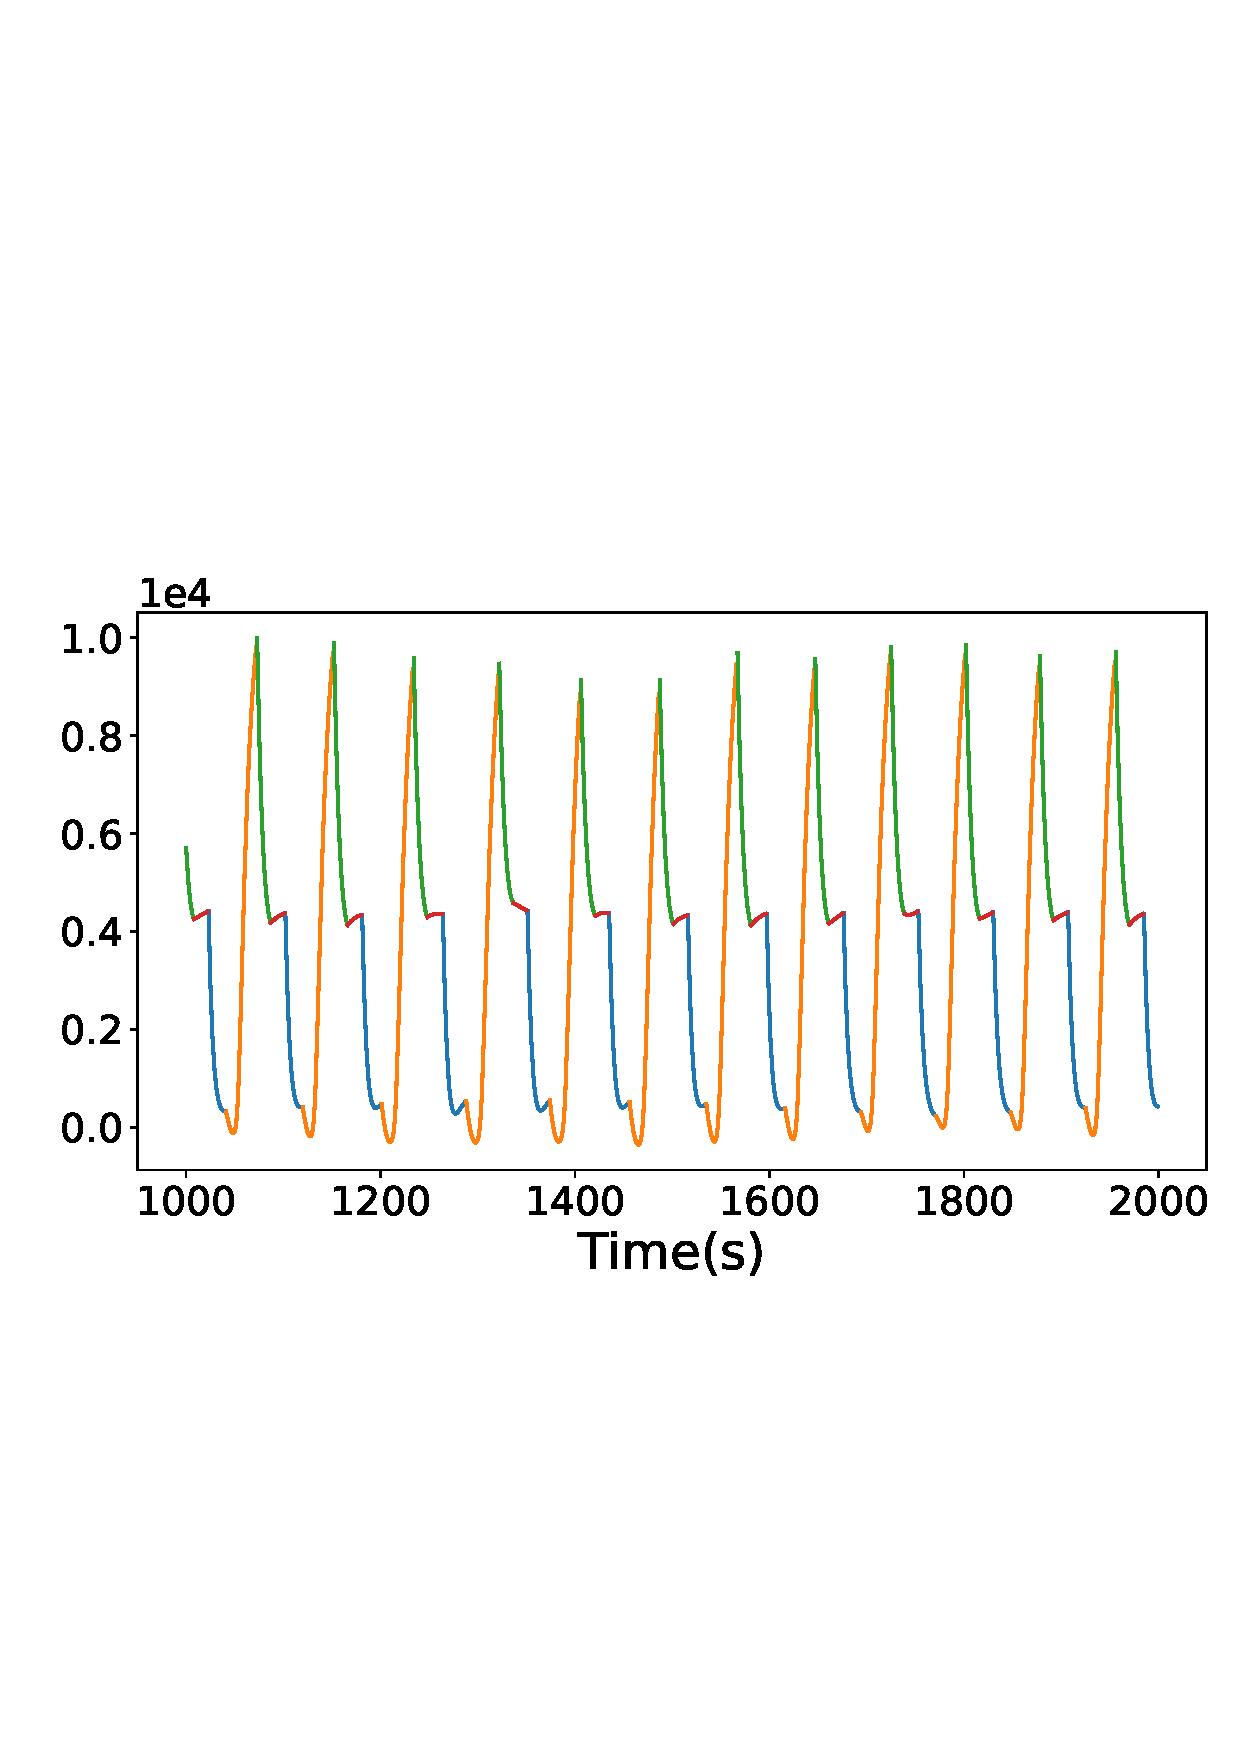
\includegraphics[width=0.45\linewidth]{figures/chapter4/18.pdf}} 
\caption{在不同温度下限设定值下的进气口温度的仿真值}
% \caption{The simulations of instant cooling power under different lower boundary of temperature set points}
%\caption{The simulated instant consumed power with different temperature lower boundaries} %图片标题
\label{fig:lowerbound_simulation}
\end{figure*}

% In Fig.~\ref{fig:temperature}, we evaluate the predicted accumulated power consumption, PUE\footnote{PUE\text{ }=${\text { Total Facility Energy }}/{\text { IT Equipment Energy }}$\cite{song2015data}}, and Coefficient Of Performance (COP)\footnote{COP\text{ }=${\text { Cooling Production }}/{\text { Power consumption }}$\cite{song2015data}} within an hour for different $Ti_{\min}$.
图~\ref{fig:4_temperature}展示了在不同$Ti_{\min}$制冷系统在一小时内的累积能耗预测值,并结合实际热负载绘制了PUE\footnote{PUE\text{ }=${\text {  总能耗 }}/{\text { 设备工作能耗 }}$\cite{song2015data}} 以及性能系数(COP)\footnote{COP\text{ }=${\text {制冷量}}/{\text { 制冷能耗}}$\cite{song2015data}}的变化曲线。
PUE代表整体总能耗(制冷能耗与工作能耗的和)与工作能耗的比。
% PUE is the ratio of the total amount of energy used by a data center facility to the energy delivered to computing equipment.
% The more close PUE is to 1, the more energy-efficient the data center is.
% COP is a ratio of the actual produced cooling to required energy consumption.
PUE越接近1,说明整套制冷系统越节能。
COP是实际产生的制冷量与制冷所需能耗的比值。

% When the lower threshold is increased from ${12}^{\circ} \mathrm{C}$ to ${18}^{\circ} \mathrm{C}$, the total energy consumption declines at first and then gradually goes up after certain points.
当温度下阈值从${12}^{\circ} \mathrm{C}$增加到${18}^{\circ} \mathrm{C}$时,制冷系统总能耗先下降然后逐渐上升。
% Since the higher $Ti_{\min}$ setting narrows the gap between the upper and the lower thresholds, which makes the compressor restart more frequently. Even though the restarting process has short duration, compressor has extremely high power. 
适当增加$Ti_{\min}$时,可以有效地避免过度制冷,从而减少能耗。
但是过度增加$Ti_{\min}$会缩小温度上下限之间的间距,使得压缩机更频繁地重启。虽然重启时间较短,但此时压缩机功耗是极高的。
% As a result, from certain point on, the energy consumption accumulated during compressor restarting process accounts for an important portion, and total energy consumption goes up after that. This certain point is actually the optimal $Ti_{\min}$ that we are searching for.
当达到某一温度后,由于压缩机重新启动所需的能耗占据了制冷系统总能耗的主要部分,此后继续升高$Ti_{\min}$会使总能耗增加,这一拐点就是寻找的最佳$Ti_{\min}$。
当$Ti_{\min}$达到某一温度后,由于压缩机频繁重启增加的能耗与减少过度制冷节省的能耗持平时,此后继续升高$Ti_{\min}$会使总能耗增加。这一拐点就是本项工作希望寻找的最佳$Ti_{\min}$。
% For the three experiments with different heat loads, the optimal $Ti_{\min}$, where the total energy consumption is minimized are marked in Fig.~\ref{fig:energy}. 
对于三个不同热负载的数据集,图~\ref{fig:energy}中标出了使总能耗最小的最佳的$Ti_{\min}$。
% In Fig.~\ref{fig:pue}, the optimal temperature thresholds are consistent with the ones in Fig.~\ref{fig:energy}.
% In Fig.~\ref{fig:cop}, COP decreases with the increase of $Ti_{\min}$. 
% The reason is that frequent on-off operations reduce the time for stable cooling. 
在图~\ref{fig:4_temperature}\subref{fig:pue}中,最佳温度阈值与图~\ref{fig:4_temperature}\subref{fig:energy}中的阈值一致。
在图~\ref{fig:4_temperature}\subref{fig:cop}中,COP随着$Ti_{\min}$的增加不断降低。其原因为频繁的压缩机开闭过程会减少稳定制冷的时间,进而导致单位功耗产生的制冷量下降。
% We take it for granted that the COP is lower when system is unstable.
% When the cooling system runs unstably for a long time, the COP decreases naturally.
% The decline tendency in COP also explains why the required cooling decreases while the energy consumption increases.
COP的下降趋势也解释了为什么提高温度下限值能够使所需的冷气量减少而总制冷能耗却增加。

% 仿真结果如图.~\ref{fig:temperature}所示,曲线中标出了系统达到最小功耗时的温度下限设定值。
与此同时我们发现,最优温度设定点随热负载的增加而增加。因为热负载较高时,制冷系统在\text{On}阶段需要工作更长的时间才能使温度降低到$Ti_{\min}$,变相地增加了制冷阶段在完整工作周期中的占比。
这一发现也在一定程度上表明制冷系统的PUE与制冷、待机两阶段时长的比例具有很强的相关性。

基于仿真实验推导出的最优温度设置点$Ti^*_{\min}$,表~\ref{tab:power_save_percent}展示了优化温度设定点可以节省的功耗百分比。
表~\ref{tab:power_save_percent}展示了基于仿真实验推导出的最优温度设置点$Ti^*_{\min}$以及通过优化温度设定点可以节省的功耗百分比。
根据仿真结果,采用新的温度下限设定值可以节省约6-25\%的能耗,特别对于高热负载情况下的能耗优化是极其显著的。
因为实验\ref{sec:case-study1}中评估了模型预测累积能耗的相对百分比误差小于5\%,可以认为本节对于不同温度下限设定值的仿真结果有足够的可信度。
在未来的工作中,将进一步验证该温度设定策略在实际工业制冷系统中的能耗优化表现。

% The simulations are shown in 图.~\ref{fig:temperature}, and the optimal lower temperature set point, which can achieve the least energy consumption are marked in the curves. 
% It can be found that, optimal temperature set points are varied with the heat load, higher heat load corresponding to higher optimal temperature set points. 
% Based on the inferred optimal set points, the percentage of the saved energy is simulated and shown in \ref{tab:power_save_percent}.
% From results, we find that optimizing the lower boundary set point will produce great energy saving. 
% It is an extremely economical and green improvement of the studied data center, which is supposed to be verified in the future work.

\begin{table}[]
\centering
\caption{能耗优化效果}
\label{tab:power_save_percent}
\begin{tabular}{lcccc}
\hline
\multicolumn{1}{c}{\textbf{不同负载的数据集}} & 1.7k  & 3.8k    & 6.3k  \\ \hline
最优温度设定值(${ }^{\circ} \mathrm{C}$)               & 14   & 15     & 15.5    \\
最大功耗优化比例(\%)              & 6.49 & 10.93  & 25.71\\ \hline
\end{tabular}
\end{table}


% optimized power,best temp set point is the temperature point when the power consumption is the lowest ,max optimized power is compare the lowest power consumption with the truth power consumption



% \begin{table*}[]
% \centering
% \caption{rrse(1.7k)}
% \label{tab:rrse(1.7k)}
% \begin{tabular}{lccc}
% \hline
% \textbf{\%RRSE(1.7k)} & Ti    & PCooling & Power Cooling \\ \hline
% H-ODE                 & 14.32  & 17.34    & 19.37        \\
% ODE-RNN               & 16.33  & 18.86    & 16.79        \\ \hline
% \end{tabular}
% \end{table*}

% \begin{table*}[]
% \centering
% \caption{rrse(3.8k)}
% \label{tab:rrse(3.8k)}
% \begin{tabular}{lccc}
% \hline
% \textbf{RRSE(3.8k)} & Ti    & PCooling & Power Cooling \\ \hline
% H-ODE               & 12.77 & 14.60    & 17.79         \\
% ODE-RNN             & 15.37 & 15.25    & 16.97         \\ \hline
% \end{tabular}
% \end{table*}



% \begin{table*}[]
% \centering
% \caption{rrse(4.2k)}
% \label{tab:rrse(4.2k)}
% \begin{tabular}{lccc}
% \hline
% \textbf{RRSE(4.2k)} & Ti    & PCooling & Power Cooling \\ \hline
% H-ODE               & 13.34 & 15.57    & 18.88         \\
% ODE-RNN             & 17.03 & 18.61    & 17.54         \\ \hline
% \end{tabular}
% \end{table*}

% \begin{table*}[]
% \centering
% \caption{rrse(6.3k)}
% \label{tab:rrse(4.2k)}
% \begin{tabular}{lccc}
% \hline
% \textbf{RRSE(6.3k)} & Ti    & PCooling & Power Cooling \\ \hline
% H-ODE               & 13.07 & 15.65    & 19.29         \\
% ODE-RNN             & 17.75 & 18.61    & 18.23         \\ \hline
% \end{tabular}
% \end{table*}


% \begin{figure}
% \centering
% \subfigure[The time of state-off]{\includegraphics[width=4cm]{figures/chapter4/state1.png}}
% \subfigure[The time of state-on]{\includegraphics[width=4cm]{figures/chapter4/state4.png}}
% \caption{The data of the four data sets are generated at different power of the server, which are 1.7kw, 3.8kw, 4.2kw and 6.3kw respectively. Compare the duration time of system on and off under different power.} %图片标题
% \label{fig:state}  %图片交叉引用时的标签
% \end{figure}

\begin{figure*}[htb]
    \centering
    \subfigure[制冷能耗]{\includegraphics[width=0.7\linewidth]{figures/chapter4/power.pdf}\label{fig:energy}}
    \subfigure[PUE]{\includegraphics[width=0.7\linewidth]{figures/chapter4/pue.pdf}\label{fig:pue}}
    \subfigure[COP]{\includegraphics[width=0.7\linewidth]{figures/chapter4/cop.pdf}\label{fig:cop}}
    % \includegraphics[width=8cm]{figures/temperature.eps}
    \caption{在不同热负载下改变温度设定下限值对功耗、COP、PUE的影响}
    \label{fig:4_temperature}
    % \vspace{-10pt}
\end{figure*}

\section{本章小结}
\label{sec:4_conclusion}
本章针对连续时间周期跳变系统的建模预测问题,提出了一种基于自跳跃常微分方程模型,同时基于该模型构建了用于系统开环预测的编码器-解码器框架。
% 该模型能够对给定历史序列数据中学习系统中不同阶段下的多输入多输出动态特性,通过给定未来的系统输入能够预测系统的未来输出。
该框架能够对给定的历史序列数据进行编码,通过给定系统的未来序列输入,模型能够预测周期跳变系统的未来阶段变化以及系统输出。
% 中学习系统中不同阶段下的多输入多输出动态特性,通过给定未来的系统输入能够预测系统的未来输出。
为了使模型更好地学习跳变系统在不同阶段内的动态特性,AJ-ODE-Net包含了多个层次常微分方程网络, 每个H-ODE-Net能够独立地学习各阶段下的系统动态,并分别建模系统的稳定输出和非稳定输出。同时,AJ-ODE-Net构建阶段转换预测器以指定各个预测时刻所用的H-ODE-Net。
% 作为ODE-Net的扩展,H-ODE-Net中的双层结构分别用于估计隐状态的导数和系统输出的导数,并且对于稳定输出和非稳定输出采用不同的导数模块进行建模。
% 基于AJ设计的阶段转换预测器将系统的先验知识集成为转换规则,以提高模型的预测精度和可解释性。
最后,本章利用所提出的基于AJ-ODE-Net的编码器-解码器框架建模某一工业制冷系统。
与其他方法相比,AJ-ODE-Net能够很好地预测制冷系统温度、功耗变化,并且能够准确地预估阶段转换点。
% Furthermore, we search the optimal lower threshold set points for the inlet temperature for minimizing cooling energy consumption with different heat loads.
此外,
本章依托于训练得到的能耗仿真模型,成功优化了制冷系统的温度下限设定点,有效减少了不同热负荷下的制冷能耗。
% It is shown that up to 25\% energy can be saved by adopting the optimized settings obtained by the simulations.
仿真结果表明,采纳优化后的温度阈值可以节省高达6-25%的制冷能耗。
% The proposed AJ-ODE-Net could be deployed forward to model general continuous-time markov jump systems, future works will be devoted to extend the deterministic stage prediction to markov process.
% 本章所提出的AJ-ODE-Net可以被应用于一般的连续时间马尔科夫跳跃系统的模型中,未来的工作将致力于将确定性的阶段预测扩展到带有随机性的马尔科夫过程。
% Moreover, instead of designing transition rules manually in complex systems, we consider to further develop more intelligent stage labeling solutions based on unsupervised machine learning methods~\cite{10.1145/3097983.3098060}.

在未来的研究工作中,可以尝试将AJ-ODE-Net推广至更通用的马尔科夫连续时间跳变系统,将固定的周期转换过程推广至随机的马尔科夫链。
另外,本文采用自定义状态转移规则的方式对原始系统输出序列进行阶段标注。未来将考虑引入无监督统计学习方法,实现更加智能的自动标注~\cite{10.1145/3097983.3098060}。





% 此外,基于训练得到的仿真模型实现了对于制冷系统的能耗仿真。实验结果表明,当预测时间超过35分钟时,能够基本消除了相位误差的影响,模型能够较为准确地估计预测时间内的系统能耗。另外,该模型能够仿真触发制冷启动的温度设定值对于系统能耗的影响,进而求解使冷却能耗最小的最优温度设定值。通过对不同服务器负载数据进行模拟,给出了不同负载下的最优温度设定,并预估经过优化的设定值能够节省制冷系统能耗约29\%。


% In this paper, a novel deep learning based framework AJ-ODE-Nets is proposed, target at modeling periodic and multi-stage industrial complex systems. It is a MIMO framework, at first place, the framework learns the system behavior and stage transitions during given duration of conditional range, then start to predict required variables with given inputs. AJ-ODE-Net serves as the key module, which takes in inputs, generates hidden states and appoints the system to switch across different ODE-Nets. In order to better characterize different and hybrid physical processes, Hierarchical Neural ODE networks (H-ODE-Net) are adopted to fit different stages of the system, which contains hybrid stationary and non-stationary structure to deal with complex and more general cases. In addition, prior knowledge is integrated and written as transformation rules into the AJ of Stage Transition Predictor. The option allows improving the model interpretability, and exploring system optimization possibilities. With the features mentioned above, AJ-ODE-Net has prominent advantages in simulating multi-stage physical processing. Finally, the proposed AJ-ODE-Net framework is implemented on a cooling system of a running data center. Comparing with other methods, AJ-ODE-Nets achieves better performance in open loop estimation for several operating variables, with accurate results for each stage including the transition point. \\
% Moreover, two applications are realized as use cases. Firstly, the framework is applied to estimate energy consumption for short and long terms cases. Evaluations show that, accurate estimation results can be obtained for prediction duration more than 35 minutes, to get rid of the impact brought by initial points (phrase difference in periodic sequences). Secondly, for the purpose of reducing cooling energy consumption, simulations are conducted by varying lower boundary temperature set points within Stage Transition Predictor to search for the optimal configuration under different heat load
% \chapter{插入参考文献}
% \section{\BibTeX 的使用}
% \BibTeX 是一种格式和一个程序,用于协调LaTeX的参考文献处理。\BibTeX 使用数据库的的方式来管理参考文献. \BibTeX 文件的后缀名为 .bib。 先来看一个例子:
% \begin{quote}
% @article\{name1,\\
% author = \{作者, 多个作者用 and 连接\},\\
% title = \{标题\},\\
% journal = \{期刊名\},\\
% volume = \{卷20\},\\
% number = \{页码\},\\
% year = \{年份\},\\
% abstract = \{摘要, 这个主要是引用的时候自己参考的, 这一行不是必须的\}\\
% \}\\

% @book\{name2,\\
% author ="作者",\\
% year="年份2008",\\
% title="书名",\\
% publisher ="出版社名称"\\
% \}
% \end{quote}
% 说明:第一行@article 告诉 \BibTeX 这是一个文章类型的参考文献,还有其它格式, 例如 article, book, booklet, conference, inbook, incollection, inproceedings,manual, misc, mastersthesis, phdthesis, proceedings, techreport, unpublished 等等。接下来的"name1",就是你在正文中应用这个条目的名称。其它就是参考文献里面的具体内容啦。
% \section{在\LaTeX 中使用\BibTeX }
% 为了在LaTeX中使用BibTeX 数据库, 你必须先做下面三件事情:
% \begin{enumerate}
% \item 设置参考文献的类型 (bibliography style). 标准的为 plain:\\
%   $\backslash$bibliographystyle\{plain\}\\
% 将上面的命令放在 \LaTeX 文档的 $\backslash$begin\{document\}后边. 其它的类型包括:\\
% unsrt – 基本上跟 plain 类型一样,除了参考文献的条目的编号是按照引用的顺序,而不是按照作者的字母顺序。\\
% alpha – 类似于 plain 类型,当参考文献的条目的编号基于作者名字和出版年份的顺序。\\
% abbrv – 缩写格式。
% \item 标记引用 (Make citations). 当你在文档中想使用引用时, 插入\LaTeX 命令$\backslash$cite{引用文章名称}。"引用文章名称" 就是前边定义@article后面的名称.
% \item 告诉LaTeX生成参考文献列表,在 LaTeX 的结束前输入$\backslash$bibliography{bibfile}。这里bibfile 就是你的 BibTeX 数据库文件 bibfile.bib .
% \end{enumerate}

% \section{运行 \BibTeX}
% 分为下面四步:
% \begin{enumerate}
% \item 用LaTeX编译你的 .tex 文件 , 这是生成一个 .aux 的文件, 这告诉 \BibTeX 将使用那些应用;
% \item 用\BibTeX 编译 .bib 文件;
% \item 再次用\LaTeX 编译你的 .tex 文件,这个时候在文档中已经包含了参考文献,但此时引用的编号可能不正确;
% \item 最后用 \LaTeX 编译你的 .tex 文件,如果一切顺利的话, 这是所有东西都已正常了.
% \end{enumerate}

% \section{本论文参考文献格式}
% 北京科技大学博士论文的参考文献要求符合国家标准“GB/T7714-2005文后参考文献著录规则”。本模板中已包含了关于符合此要求的gbt7714-2005.bst文件,只需要将参考文献类型设置为$\backslash$bibliographystyle\{gbt7714-2005\}即可。



%第五章
\include{chapter5}

% 第六章
% \pagenumbering{arabic}
\algdef{SE}[DOWHILE]{Do}{doWhile}{\algorithmicdo}[1]{\algorithmicwhile\ #1}%
\renewcommand{\b}{\mathbf}
% \floatsetup[table]{capposition=top}
% \newfloatcommand{capbtabbox}{table}[][\FBwidth]


\chapter{基于连续时间有模型强化学习的复杂工业系统优化与控制}
\section{本章引言}

在现代复杂过程工业生产中,对控制性能指标进行优化是不同控制算法、控制系统的首要任务。
在冶金、采矿领域等复杂过程工业场景下,浓密机是一种被广泛应用的大型沉降工具,它通过重力沉降作用可以将低浓度的固液混合物进行浓缩形成高浓度的混合物,起到减水、浓缩的作用。
在对浓密机进行控制时,底流浓度是核心控制指标。该参量与其他过程监控变量如进料流量、进料浓度、出料流量、泥层高度有着复杂的耦合关系。
在大部分的实际生产过程中,浓密机底流浓度的控制一般是操作员根据个人经验,通过对底流流量设定值、絮凝剂流量设定值进行调节,间接地使底流浓度追踪其工艺设定值。但是由于浓密机运行过程具有非线性、多变量、高时滞等特点,操作员难以维持底流浓度持续稳定,浓度存在偏差的底流会导致产品质量退化以及增加工业生产成本。

浓密机是一种典型的复杂过程工业设备,关于过程工业设备优化控制的研究一直是工业界、学术界研究的热点问题。
对于机械结构明确、且能够精确建立动态模型的工业设备,可以采用基于模型的优化控制方法,如:实时优化控制(realtime
optimization, RTO)\cite{Yin2014}、模型预测控制(model predictive
control,MPC)\cite{Kouro2009}等。
但由于浓密机系统机械结构复杂、部分变量难以观测,因此难以建立准确的数学模型近似其运转机理,导致基于模型的方法无法适用于此类复杂工业设备的控制。
研究人员提出了基于数据驱动的控制方法来实现对此类无模型工业设备的控制。
Dai等\cite{Dai2015}提出了用于解决赤铁矿研磨系统控制问题的数据驱动优化(Date
driven optimization, DDO)控制算法。
Wang等\cite{Wang2016}采用基于数据驱动的自适应评价方法解决连续时间未知非线性系统的无穷范围鲁棒最优控制问题。

近年来,基于强化学习\cite{Sutton2018}\cite{F.L.LewisD.Vrabie2012}理论的最优控制技术,也称为自适应动态规划(Adaptive
dynamic programming,
ADP)\cite{Prokhorov1997}\cite{Werbos2008}\cite{Duan:643}技术,是控制领域的研究热点话题。
典型的自适应动态规划算法,如HDP、双启发式动态规划(Dual heuristic
programming,DHP)、动作依赖启发式动态规划(Action dependent
heuristic dynamic programming,
ADHDP)\cite{Werbos2008}等均采用多个神经网络分别对被控系统动态模型、控制策略、策略评价模型进行建模。此类方法可以在模型未知的情况下以数据驱动的方式在线学习控制策略。
Liu等\cite{Liu2015}提出了一种在线自适应动态规划算法用来解决离散时间多输入多输出仿射系统控制问题,且该方法仅需要训练少量网络参数。Liu等\cite{LiuL2017}采用一种基于强化学习的自适应跟踪控制技术解决多输入多输出系统容错控制问题。
Xu等\cite{XuX2017}采用拉普拉斯特征映射算法提取被控系统全局特征,并将该全局特征用于DHP算法中以增强值函数网络的近似能力。

近年来,利用自适应动态规划方法解决过程工业控制问题也取得很大研究进展。
Wei等\cite{Wei2014}将煤炭气化过程的最优追踪控制转化为双人零和最优控制问题,并采用迭代自适应动态规划方法求解最优控制率,同时给出了收敛稳定性的分析。
Jiang等\cite{Jiang2018}利用穿插学习策略迭代(Interleaved Learning
Policy Iteration,
ILPL)实现了对浮选过程操作指标优化的控制,获得了比传统值函数迭代(Value
iteration, VI)、策略迭代(Policy iteration, PI)算法更佳的控制效果。
Jiang等\cite{Jiang2019}将强化学习与举升方法结合(lifting
technology),实现了对浮选过程设备层与操作层双速率系统的最优控制。

上述算法均使用被控系统实时生成的数据对神经网络进行训练,该训练方法忽略了系统在短期内产生的历史轨迹数据对模型学习的影响。同时,在工业场景下进行设备在线控制对算法实时性要求较高。上述方法对于控制量的计算均依托于表征控制策略的神经网络,而对于控制网络或动作网络的训练将产生较大的时间开销。
为了解决上述问题,本章引入了短期经验回放技术\cite{Modares2014}\cite{Mnih2013}以对短期内的系统运行轨迹数据进行回放训练。实验证明该技术有效增强了算法收敛稳定性,且在其他ADP类在线控制算法中具有通用性。同时本章根据浓密机系统特性提出了一种迭代梯度优化算法,该算法可以在没有动作网络的情况下求解控制输入量。实验表明该方法能够在提升控制精度的同时,减少模型学习过程中产生的时间消耗。



% 为了克服人工控制的缺陷,多种针对浓密机的智能控制算法被提出。
% Xu,Ning等\cite{Xu2015}利用泥层质量平衡模型与专家系统实现了对絮凝剂添加比例与底流流量设定值的控制,
% Chai等\cite{Chai2016}\cite{Wang330}将模糊控制算法与(Proportional
% Integral Differential,
% PID)控制相结合,实现对底流浓度的控制,且最大程度保持底流流量的稳定性。
% Ojeda,P等\cite{Ojeda2014}利用复杂专家系统实现了对于底流浓度与溢流水浊度的控制,并且在实际工业场景获得较好效果。
% 由于浓密机运行机理复杂,难以建立数学模型,难以应用传统控制理论、最优控制算法,大部分浓密机控制算法都是基于人工设计的专家系统或手工制定模糊控制器中的规则库

% 通过归纳现有的浓密机控制手段,可以发现由于浓密机运行机理复杂,难以建立数学模型,难以应用传统控制理论、最优控制算法,大部分的控制算法都是基于人工设计的专家系统或手工制定模糊控制器中的规则库,并辅助以传统的比例积分控制手段实现对底流泵速、絮凝剂泵速的控制。此类方法过度依赖人工经验、缺乏自适应性。

% %本章提出了基于强化学习\cite{Sutton2018}\cite{F.L.LewisD.Vrabie2012}的浓密机在线控制算法。
% 近年来,基于强化学习\cite{Sutton2018}\cite{F.L.LewisD.Vrabie2012}理论的最优控制技术(也称为自适应动态规划(Adaptive
% dynamic programming,
% ADP)\cite{Prokhorov1997}\cite{Duan:643}\cite{Jiang2018}\cite{Liu2015}
% \cite{XuX2017}\cite{LiuL2017}),在解决飞行器控制\cite{helicopters}、车辆控制\cite{Vehicles}等方面取得了很大的进展。
% 并且在过程工业控制领域中,采用强化学习方法解决工业控制场景下指标设定值追踪与智能优化控制问题的思想也催生出诸多研究成果\cite{Jiang2018}\cite{Li2018}\cite{Jiang2019}\cite{Xue2019}。
% 尽管复杂过程工业场景下外部环境因素扰动频繁、设备运行过程复杂且难以建立数学模型对其生产过程进行准确的描述,但强化学习算法具有自适应、不依赖于精确数学模型的特点,因此可以作为一种解决复杂过程工业设备优化控制问题的有效手段。

% 本章提出了基于强化学习的浓密机在线控制算法。通过设计融合评价网络与模型网络的双网结构实现对浓密机底流泵速和絮凝剂泵速的控制。
% 评价网络用于拟合折扣累计代价函数,模型网络用于对生产过程进行建模与预测。
% 为了增加控制模型在噪音量改变下的收敛速度,相比于传统HDP算法,本章在双网结构中去掉了动作网络。
% 前人研究表明\cite{Luo2016}\cite{Padhi2006},在启发式动态规划类算法中,去掉动作网络可以有效减少模型训练时间。但是在某些复杂系统控制问题中,去除动作网络会使模型难以拟合复杂策略函数,最终引起控制效果变差。
% 本章采用迭代梯度优化算法求解控制输入量,该方法不仅保留了无动作网络类ADP方法在训练时间上的优势,并且由于浓密机系统具有运行缓慢的特性,该方法在浓密机控制问题上也获得了相比传统方法更佳的控制效果。
% 此外,由于浓密机具有运行缓慢、状态迁移滞后的特点,为了维持评价网络的局部梯度差异以增强控制模型的收敛速度,本章提出了短期经验回放技术\cite{Modares2014}\cite{Mnih2013}以对短期内的系统运行轨迹数据进行回放训练。
% 实验证明该技术有效增强了算法收敛稳定性,且在其他ADP类在线控制算法中具有通用性。

本章主要贡献总结如下:
\begin{itemize}[nosep]
\item  提出了一种基于ADP算法架构的启发式评价网络值迭代算法
(Heuristic critic network value iteration,
HCNVI)。该算法仅通过评价网络、模型网络和梯度优化算法即可求解系统最优控制输入。
% \item  一种浓密机预测网络训练方法,根据进料噪音项的概率分布,对原始离线数据进行采样构建预测网络训练集,该方法可以有效增强模型网络预测精确度,并对控制模型性能产生促进作用。
\item  提出了一种适用于评价网络训练的短期经验回放技术。训练评价网络时,将短期内系统运行轨迹数据共同用于模型训练,该方法可以有效增强评价网络收敛速度。
\item  通过浓密机仿真实验验证了HCNVI算法的有效性。实验结果表明本章提出方法在时间消耗、控制精度上均优于其他对比方法。
\item  通过浓密机仿真实验验证了HCNVI算法的有效性。实验结果表明本章提出方法在时间消耗、控制精度上均优于其他对比方法。
\end{itemize}

本章内容组织如下: 
\secref{sec:formulation}对连续时间域下的复杂工业系统的控制过程进行形式化描述。
\secref{sec:ode_system_modeling}介绍了如何使用ODE-Net建模浓密机系统运行过程。
\secref{sec:ctirl}介绍了基于HCNVI算法以及如何利用该算法实现浓密机在线控制。
\secref{sec:experiment}通过两组仿真实验验证本章提出控制模型的有效性。
\secref{sec:conclusion}对本章研究工作进行总结。

\section{连续时间强化学习形式化描述}
\label{sec:formulation}
% Please add the following required packages to your document preamble:
% \usepackage{graphicx}

% \begin{table}[!ht]
% \centering
% \caption{浓密过程示意图中符号解释}
%  %英文标题begin
%     \addtocounter{table}{-1}
%     \vspace{-0.2cm}
%     %\SetEnglishCaption
%     \renewcommand{\tablename}{Table}
%     \caption{Explaination of symbols in illustration of thickening process.}
%     \renewcommand{\tablename}{表}
%     \vspace{0.4cm}
%  %英文标题end
% \begin{tabular}{@{}lll@{}}
% \toprule
% 符号 & 含义 & 单位 \\ \midrule
% DT & 密度变送器 & $kg/m^3$ \\
% FT & 流量变送器 & $m^3/h$ \\
% PT & 压强变送器 & $kPa$ \\
% AT & 浊度变送器 & $ppm$ \\
% LT & 液位变送器 & $m$ \\ \bottomrule
% \end{tabular}
% \label{tab:symble_explain}
% \end{table}
对于一般的复杂工业系统,其系统运行过程的控制效果往往根据某些监测指标的状态进行评价,假定其控制目标为$y(t) \in \mathbb{R}^n$。
该指标受控制输入、系统状态参量、及其他外部噪音扰动影响。
本节将系统可控制输入量表示为$\b u(t) \in \mathbb{R}^m$。
将非控制输出量表示为$\b h(t) \in \mathbb{R}^l$,该参量是表征当前系统状态的重要参量,它可被间接控制但不作为控制目标。
由于在部分工业场景中,上游工序产生的物料性质是不可控的。为了使提出的控制模型具有通用性,因此本章引入噪音输入量$\b c(t) \in\mathbb{R}^d$以定义那些会对生产系统产生影响的、可被监测,但无法被控制的监测量。
因此,浓密机系统可表述为\equref{equ:system_dynamic}形式的非线性系统,其中$f
( \cdot )$为未知非线性函数。
\begin{equation}\label{equ:system_dynamic_dt}
    [\b y ( t_{k + 1} ), \b h(t_{k+1})]^{\rm T} = f ( \b y(t_k), \b u ( t_k ) ,\b c ( t_k ) ,\b h(t_k), t_{k+1}-t_k)
\end{equation}
定义系统状态量$\b s(t)=[\b y(t), \b h(t)]^T$。从连续时间域角度,动态系统可以进一步写成如下形式:
\begin{equation}
\dot{\b{s}}(t)=\frac{d \b{s}(t)}{d t}=\b{f}(\b{s}(t), \b{u}(t))
\end{equation}
函数$\mathbf{f}: \mathbb{R}^{n+m+l+d} \mapsto \mathbb{R}^{n+l+d}$描述了系统当前状态与外部输入量到系统状态导数$\boldsymbol{\dot s}(t)$的映射。
在任意实值时间$t\in R_{+}$的系统状态依赖于初始状态$\b s_0$以及外部输入信号$\b u[0,t)$的无穷小序列。求解过程为:
\begin{equation}
\label{equ:system_dynamic_ct}
\mathbf{s}(t)=\mathbf{s}_{0}+\int_{0}^{t} \mathbf{f}(\mathbf{s}(\tau), \mathbf{u}(\tau)) d \tau,
\end{equation}
其中$\tau$为辅助时间变量。

对于系统运行过程\equref{equ:system_dynamic_ct},本章提出的连续时间域下复杂工业系统控制算法可以根据任意时刻系统状态量$\b s(t)$,实时给出最优的控制输入量$\b u^*(t)$,
使系统输出$y(t)$追踪其设定值$y^*(t)$。另外,为了保证系统运行安全与仪器寿命,控制输入量必须满足一定的限制条件。因此,定义控制系统效用函数为:
\begin{equation}
U(\b s(t), \b u(t))=\left(y(t)-y^{*}(t)\right)^{T}Q\left(y(t)-y^{*}(t)\right)+\left(u(t)-{u_{m i d}}\right)^{T} R\left(u(t)-{u_{m i d}}\right)
\label{equ:U}
\end{equation}
效用函数代表了在当前状态$\b s(t)$下,执行控制输入${\b u}(t)$需要承受的代价。$Q$、$R$是对称正定矩阵。$\b u_{mid}=\dfrac{\b u _ { \max } + \b u _ { \min }}{2}$,$u _{\min}$,$u _{\max}$分别代表$u(t)$的上限和下限,。

连续时间(CT)控制的目标为在满足控制约束下,最小化效应函数在无穷时间范围下的积分$\int_{t}^{\infty} U(\mathbf{s}(\tau), \mathbf{a}(\tau)) d \tau$。综上本章将其转化为有约束的无穷范围折扣累积代价积分最优化问题:
\begin{equation}
\label{equ:goal}
\begin{aligned}
&{\min_{\b u[t,\infty)}} \quad V(\mathbf{s}(t))=\int_{t}^{\infty} e^{-\frac{\tau-t}{\eta}} U(\mathbf{s}(\tau), \mathbf{u}(\tau)) d \tau \\
& \rm{s.t.} \quad \dot{\b{s}}(t)=\b{f}(\b{s}(t), \b{u}(t)),{{\b u}_{\min }}\le {\b {u}}(t)\le {{\b u}_{i\max }}
% \begin{matrix}
%    \dot{\b{s}}(t)=\b{f}(\b{s}(t), \b{u}(t))  \\
%    {{\b u}_{\min }}\le {\b {u}}(t)\le {{\b u}_{i\max }} \\
%    \end{matrix}
\end{aligned}
\end{equation}
$V(\b s(t))$为折扣累计评价值函数,用于在给定控制策略下,从长期角度评估控制策略的好坏。
$\eta$是折扣因子。
% $u _{i\min}$,$u _{i\max}$分别代表对$u _ { i } ( k ) $的限制,
对于有约束的优化问题\equref{equ:goal},由于复杂系统$\b f$未知,且具有非线性特性。难以利用动态规划或其他最优化方法求解最优的$\b a(t)$。因此本章提出连续时间强化学习方法HCNVI,以解决上述最优控制问题。该方法充分利用浓密机系统运行缓慢的特性,能够在在线控制的情况下,根据系统闭环反馈数据学习最优控制策略,逐渐优化效用函数。
% 具体地,其目标为构建策略函数:
% \begin{equation}
%     \b{u}(t)=\pi(\b{s}(t))
% \end{equation}
\section{启发式评价网络值迭代算法}
本章提出的启发式评价网络值迭代算法(HCNVI)为有模型强化学习算法。进行策略学习之前,首先需要对系统动态进行辨识。完成动态系统的学习后,模型能够从在线控制过程中收集数据进行评价网络的训练。
伴随着控制过程中的数据采集与参数更新,模型逐渐达到收敛,系统逐渐被控制到最优态。接下来,本节将从系统动态模型网络构建、评价网络构建、动作生成、经验回放四个方面介绍HCNVI算法的实现过程。
\subsection{基于常微分方程网络的系统模型构建}
\label{sec:ode_system_modeling}
本节将介绍构如何利用离线数据训练被控系统的预测模型。
假设离线数据集共包含$N$组状态-控制轨迹:$\mathcal{D}=\left\{\left(\mathbf{s}_{0: T}^{(n)}, \mathbf{a}_{0: T}^{(n)}\right)\right\}_{n=1}^{N}$,每条轨迹数据均采样于被控系统的实际生产过程。本节将利用该数据训练ODE-Net模型,以近似真实被控系统的运行过程。

对于观测时间点$t_{0: T}$,轨迹中的第$i$个观测表示为$\mathbf{s}_{i}:=\mathbf{s}\left(t_{i}\right)$。与下一观测采样时间的间隔定义为$\Delta t = t_{i+1}-t_i$。所述预测模型构建方法允许观测时间间隔是非均匀的。
类似于本章的第二、三、四章,本章采用带有参数$\theta$的深度神经ODE模型$\hat{\b{f}}_\theta$估计真实系统的状态微分,进而可以通过前向求解仿真ODE-Net轨迹的方式精确地重现真实系统ODE方程的轨迹。
其学习目标为求解最优ODE参数$\theta^*$以最大化数据集的对数似然:
% \begin{equation}
%     \theta^* = \arg\max_{\theta}\log p(\mathcal{D}|\theta)=\sum_{n=1}^{N} \sum_{i=0}^{T} \log \mathcal{N}\left(\mathbf{s}_{i}^{(n)} \mid \hat{\mathbf{s}}_{i}^{(n)}, \Sigma\right)
% \end{equation}
\begin{equation}
\label{equ:likelihood}
    \mathcal{L}(\theta, \mathcal{D})=\sum_{n=1}^{N} \sum_{i=0}^{T} \log \mathcal{N}\left(\mathbf{s}_{i}^{(n)} \mid \hat{\mathbf{s}}_{i}^{(n)}, \Sigma\right)
\end{equation}
其中$\Sigma$为可训练的观测噪音协方差矩阵。通过前向仿真ODE-Net模型$\hat{\mathbf{f}}_{\boldsymbol{\theta}}(\mathbf{s}, \mathbf{u})$获得轨迹采样$\hat{\mathbf{s}}_{0:T}$:
\begin{equation}
\label{equ:state_traj}
\hat{\mathbf{s}}_{i}^{(n)} \mid\left(\mathbf{s}_{0}^{(n)}, \mathbf{u}_{0: t}^{(n)}\right)=\mathbf{s}_{0}^{(n)}+\int_{0}^{t_{i}} \hat{\mathbf{f}}_{\boldsymbol{\theta}}\left(\hat{\mathbf{s}}_{\tau}^{(n)}, \mathbf{u}_{\tau}^{(n)}\right) d \tau
\end{equation}

\equref{equ:state_traj}求解的状态轨迹完全依赖于积分时给定的初始状态$\b s_0$以及连续时间过程的动作序列$\b u[0:t)$。由于数值积分过程可能在任意时间点上进行评估,因此需要保证动作信号在时间域上是连续的。本节采用带有二次平方指数核函数的核插值方法对数据集中离散的动作序列$\mathcal{D}_{\mathbf{a}}=\left\{\mathbf{a}_{0: T}^{(n)}\right\}_{n=1}^{N}$进行插值处理。

对于给定的非均匀采样控制信号$\{(t_i, \b u _i)|i=1\cdots N\}$,$\b t = (t_1,t_2,\cdots,t_N)^T$,$\b U = (\b u_1,\b u_2,\cdots,\b u_N)^T$,可以估计高斯过程(Gaussian Process, $\mathcal{GP}$)。首先,基于平方指数(Squared exponential, SE)核函数定义控制信号的协方差矩阵$\b K(\b t, \b t)\in\mathbb{R}^{N\times N}$,其中:
\begin{equation}
K(t_p, t_q) = \exp \left(-\frac{1}{2}\frac{\left|{t}_{p}-{t}_{q}\right|}{\ell}^{2}\right)
\end{equation}。
对于给定待插值时间点$t_*$,其控制信号$\b u(t_*)$的后验分布满足高斯分布:
\begin{equation}
\begin{aligned}
    \hat{\b {u}}(t_*)\sim \mathcal{N}(&\mathbf{K}(t_*,\mathbf t)^{\top}\left(K(\mathbf t,\mathbf t)^{-1}+\sigma_{n}^{2} I\right)^{-1} \mathbf{U}) \\
    &K\left(t_{*}, t_{*}\right)-K\left(t_{*}, \mathbf t\right) K(\mathbf t, \mathbf t)^{-1} K\left(\mathbf t, t_{*}\right)
\end{aligned}
\end{equation}
为了确保ODE-Net计算过程稳定,需要保证估计的$\hat{\b u}(t_*)$连续,因此将高斯分布均值$E\left[\bar{\b u}(t_*)\right]$作为\equref{equ:state_traj}中求解状态轨迹时输入的控制信号。

% \begin{algorithm}[hpbt]

% \caption{基于随机$\mathcal{GP}$过程的控制信号插值} %算法的名字
% \label{alg:dyn}
% \hspace*{0.02in} {\bf 输入:} %算法的输入, \hspace*{0.02in}用来控制位置,同时利用 \\ 进行换行
% 训练集,非均匀采样的控制信号$\{(t_i, \b u _i)|i=1\cdots N\}$,$\b t = (t_1,t_2,\cdots,t_N)^T$,$\b U = (\b u_1,\b u_2,\cdots,\b u_N)^T$ \\
% 代插值的时间点 $t_*$
% % 给定共包含$N$组轨迹的原始数据集$\mathcal{D}=\left\{\left(\mathbf{s}_{0: T}^{(n)}, \mathbf{u}_{0: T}^{(n)}\right)\right\}_{n=1}^{N}$
% \hspace*{0.02in} {\bf 输出:} %算法的输入, \hspace*{0.02in}用来控制位置,同时利用 \\ 进行换行
% 差值函数$g:\left[t_{1}, t_{N}\right] \rightarrow \mathbb{R}^{M}$

% \begin{algorithmic}[1]
% \State 基于平方指数(Squared exponential, SE)核函数定义控制信号的协方差矩阵$\b K(\b U, \b U)\in\mathbb{R}^{N\times N}$,其中:
% \begin{equation}
% \b K(\b u_p, \b u_q) = \exp \left(-\frac{1}{2}\frac{\left|\mathbf{x}_{p}-\mathbf{x}_{q}\right|}{\ell}^{2}\right)
% \end{equation}
% \State 
% \begin{equation}
% \begin{aligned}
%     \bar{\b u_*}\sim \mathcal{N}(&\mathbf{K}(t_*,\boldsymbol t)^{\top}\left(K(\boldsymbol t,\boldsymbol t)^{-1}+\sigma_{n}^{2} I\right)^{-1} \boldsymbol{U}) \\
%     &K\left(t_{*}, t_{*}\right)-K\left(t_{*}, \boldsymbol t\right) K(\boldsymbol t, \boldsymbol t)^{-1} K\left(\boldsymbol t, t_{*}\right)
% \end{aligned}
% \end{equation}
% 为了确保ODE-Net计算过程稳定,需要保证$\bar{\b u}(*t)$连续,直接取均值$\mathbf{K}(t_*,\boldsymbol t)^{\top}\left(K(\boldsymbol t,\boldsymbol t)^{-1}+\sigma_{n}^{2} I\right)^{-1} \boldsymbol{U}$
% \end{algorithmic}
% \end{algorithm}

基于ODE-Net的预测模型训练过程如\algref{alg:dyn}所示。

\begin{algorithm}[hpbt]

\caption{ODE模型网络学习过程} %算法的名字
\label{alg:dyn}
\hspace*{0.02in} {\bf 输入:} %算法的输入, \hspace*{0.02in}用来控制位置,同时利用 \\ 进行换行
给定共包含$N$组轨迹的原始数据集$\mathcal{D}=\left\{\left(\mathbf{s}_{0: T}^{(n)}, \mathbf{u}_{0: T}^{(n)}\right)\right\}_{n=1}^{N}$

\begin{algorithmic}[1]
\For{$i=1,\cdots,Epochs$} % For 语句,需要和EndFor对应
% \State 根据当前值函数 $V_i(\cdot)$寻找最优控制策略
\State 从$\mathcal{D}$中随机采样$N_d$个子序列,每个时间长度为$t_s$:
\begin{flalign}
\mathcal{D}^{\prime}=\left\{\left(\mathbf{s}_{t_{n}: t_{n}+t_{\mathrm{s}}}^{(n)}, \mathbf{a}_{t_{n}: t_{n}+t_{s}}^{(n)}\right)\right\}_{n \in \Xi}, \Xi \subset\{1, \ldots, N\},|\Xi|=N_{\mathrm{d}}, t_{n} \sim \mathcal{U}\left[0, T-t_{s}\right]
\end{flalign}
\State 对$\mathbf{a}_{t_{n}: t_{n}+t_{s}}^{(n)}$进行插值,构建连续信号$\mathbf{a}[t_{n}, t_{n}+t_{s})^{(n)}$
\State 由\equref{equ:state_traj}求解$\{\hat{\mathbf{s}}_{t_n:t_n+t_s}^{(n)}\}_{n \in \Xi}$
\State 由\equref{equ:likelihood},计算ODE网络梯度$\nabla_\theta \mathcal{L}(\theta, \mathcal{D})$,采用梯度提升优化$\boldsymbol{\theta}$
\EndFor

\end{algorithmic}
\end{algorithm}









% 本小节将基于算法\ref{alg:VI},提出一种启发式评价网络值迭代算法。
% 该算法能根据浓密机系统产生的实时监测数据$\b
% x(k)$进行在线学习,并产生满足$\Omega_{\b u}$约束的控制输入量${\b
% u}(k)$,且最小化$J(k)$。
% %该控制模型以HDP算法架构为基础,利用两个神经网络分别近似折扣累计代价函数与模型动态,并采用一种新颖的梯度迭代方法求解\equref{equ:VI_u}。
% 算法整体结构如图\ref{fig:alg_structure}所示。
% HCNVI算法中包含两个神经网络,分别是模型网络和评价网络。神经网络均采用单隐层人工神经网络,其基本结构如图\ref{fig:nn_structure}所示。
% 模型网络的训练全部离线进行,在控制任务开始后,将不再对模型网络参数进行调整。
% 控制动作决策算法根据浓密机实时反馈状态$\b x(k)$计算控制变量${\b
% u}(k)$并用于浓密机系统控制,$\b u(k),\b
% x(k)$被放入短期经验数据暂存区存储。模型训练时,由短期经验暂存区提供训练数据供模型训练。算法学习过程中,仅评价网络参数发生改变。
% \begin{figure*}[!ht]
%     \centering
%     \includegraphics[width=17cm]{figures/chapter6/fig2.eps}
%     \caption{HCNVI算法结构示意图}

% %%%%%%%%%%%%%英文标题begin
%   \addtocounter{figure}{-1}
%   \vspace{-5pt}
%   %\SetEnglishCaption
%   \renewcommand{\figurename}{Fig.}
%   \caption{Structure diagram of algorithm HCNVI}
%   \renewcommand{\figurename}{图}
% %%%%%%%%%%%%%英文标题end

%     \label{fig:alg_structure}
% \end{figure*}
% \subsection{基于ODE-Net的系统预测网络}
% 建立模型网络用来对系统动态进行建模,根据当前系统状态、外部噪音量、控制输入、预测下一时刻底流浓度和泥层高度变化。网络结构仍采用单隐层神经网络,如图\ref{fig:nn_structure}所示。模型网络具体定义如下:


% \begin{equation}
% \label{modelNN} [\hat{y}(k+1), \hat{h}(k+1)]^{\rm T}=W_{m 2} \tanh
% \left(W_{m 1}( \b \phi(k))\right)
% \end{equation}
% 其中$\b \phi (k)=[\b x(k)^{\rm T}, \b u(k)^{\rm T}]^{\rm T}$,\\
% 网络输入层包含6个节点,隐层包含20个节点,输出层2个节点,$ W _ { m1
% }$和$ W _ { m 2 }$内各个参数均初始化为$-1\sim 1$之间的随机数。
% 通过梯度下降方法训练模型网络:
% \begin{equation}
% \label{equ:train_modelnn} W_{mi}(k)=W_{m i}(k)-l_{m } \frac{\partial
% E_{m}(k)}{\partial W_{m i}(k)}
% \end{equation}
% 损失函数$E_{m}(k)$定义为:
% \begin{equation}
% \label{equ:loss_modelnn} E_{m}(k)=\frac{1}{2} \b e_{m}^{\rm
% T}(k)\b L_{m}\b e_{m}(k)
% \end{equation}
% \begin{equation}
% \label{em_modelnn}
% \begin{aligned} e_{m}(k)&=[\hat{y}(k+1), \hat{h}(k+1)]^{\mathrm{T}}-\\ &[y(k+1),h(k+1)]^{\mathrm{T}} \end{aligned}
% \end{equation}
% %e_{m}(k) = \left[[\hat{y}(k+1),\hat{h}(k+1)]^{\mathrm{T}}- \\ [y(k), h(k)]^{\mathrm{T}}\right]


% 对于模型网络,同样采用\equref{equ:normalize}对训练数据进行放缩。
% 模型网络的训练全部离线进行,在控制任务开始后,将不再对模型网络进行调整。
\subsection{基于积分强化学习的策略评价}
% 连续时间自适应动态规划算法
\label{sec:ctirl}
本节采用积分强化学习算法\cite{Guo2019}构建策略评价模型。
对\equref{equ:goal}中定义的折扣积分奖赏,可以表示为\equref{equ:J_bellman}贝尔曼方程的形式:
% 求解理想情况下最优控制输入$\b u^*(k)$。
\begin{equation}
  \hat{V}^{H}\left(\mathbf{s}_{0}\right)=\left[\int_{0}^{H} e^{-\frac{\tau}{\eta}} U(\hat{\mathbf{s}}(\tau), \hat{\mathbf{a}}(\tau)) d \tau+e^{-\frac{H}{\eta}} {V}\left(\hat{\mathbf{s}}_{H}\right)\right]
  \label{equ:J_bellman}
\end{equation}
其中$H$为任一积分范围,$\b s_H$ 为$H$时刻的终止状态。
。根据贝尔曼最优原则,$\b s_0$所在时刻的最优评价值函数$V^*(s_0)$满足连续哈密顿-雅可比-贝尔曼方程:
\begin{equation}
\label{equ:J_star} 
V ^ { * } \left( s_0 \right) = \min _{ \mathbf u[0:H ] } \{ \int_0^H e^{-\frac{\tau}{\eta}} U(\hat{\mathbf{s}}(\tau), \hat{\mathbf{u}}(\tau)) d\tau  + e^{-\frac{H}{\eta}} \hat{V}^*\left(\hat{\mathbf{s}}_{H}\right)\}
\end{equation}
对于任意范围$[0:H]$,最优的控制输入$\b a^*[0:H]$可以表示为:
\begin{equation}
\b u^*[  0:H ] \left( k \right) =\arg \min _ { \b u[0:H ] }\{ \int_0^H e^{-\frac{\tau}{\eta}} U(\hat{\mathbf{s}}(\tau), \hat{\mathbf{u}}(\tau))  + e^{-\frac{H}{\eta}} \hat{V}^*\left(\hat{\mathbf{s}}_{H}\right)\}
\label{equ:VI_u}
\end{equation}
% 由于\equref{equ:system_dynamic}中$f(\cdot)$是未知的,因此可以采用值迭代算法寻找最优控制策略,定义
% ,$\Omega _ u = \{u:u _ { \text {  min } } \leq u \leq u _ { \text {
%     max } }\}$,$x[k]=[y(k),  h(k),c ( k )^{\rm T} ]^{\rm T}$

% 由于\equref{equ:system_dynamic}中$f(\cdot)$是复杂非线性函数,无法直接对\equref{equ:J_star}进行求解,但可以利用算法\ref{alg:VI}以值函数迭代的方式求解最优值函数和最优控制律,其中$\b s(t_k)$用于表征$t_k$时刻的系统状态。根据文献\cite{Wang2012-GDHP},可以证明当$i\rightarrow
% \infty$时,值函数$V _ { i } \rightarrow V ^ { * }$,控制律$\b u _
% { i } \rightarrow \b u ^ { * }$。
% \begin{algorithm}[hpbt]

% \caption{值迭代算法} %算法的名字
% \label{alg:VI}
% \hspace*{0.02in} {\bf 初始化:} %算法的输入, \hspace*{0.02in}用来控制位置,同时利用 \\ 进行换行
% 随机定义 $V_0(\cdot)$
% \begin{algorithmic}[1]
% \State 定义控制约束集合$\Omega _ {\b u} = \{\b u:\b u _ {
% \text {  min } } \leq \b u \leq \b u _ { \text {     max } }\}$
% \For{$i=0,1,2,...,\infty$} % For 语句,需要和EndFor对应
% % \State 根据当前值函数 $V_i(\cdot)$寻找最优控制策略
% \State 策略改进
% \begin{flalign}
%     \label{equ:VI_u}
%         & \b u _ { i } \left( t \right) = \arg\min_{\b u(t)}\in \Omega_{\b u} U(y(t),\b u(t)) + \gamma V _ { i } (\b s(t))
% \end{flalign}
%   \State 策略评估
% \begin{flalign}
% \label{equ:VI_v}         V _ { i + 1 } \left( \b x(k) \right)
% = U(y(k),\b u_i(k)) + \gamma V _ { i } (\b x(k+1))
% \end{flalign}
% \EndFor

% \end{algorithmic}
% \end{algorithm}

% \subsection{基于积分强化学习的连续时间Actor-Critic算法}

通过对\equref{equ:VI_u}进行优化即可获得最优控制策略,在\equref{equ:VI_u}等号右侧的第一项为积分奖赏项。
% 类似于\eqref{equ:state_traj},利用训练得到的ODE-Net对产生的系统轨迹进行奖赏积分评估即可求得。
可以通过\eqref{equ:state_traj}预测系统轨迹,并对奖赏函数进行积分获得。
第二项为无穷积分项,无法显式求解,因此本章引入值函数近似的方法以评估未来的积分奖赏项。
具体地,HCNVI采用一个被称为评价网络的神经网络$V_\xi(\cdot)$来近似某一策略的评价函数。
神经网络选择单隐层全连接神经网络:
% ,其基本结构如图\ref{fig:nn_structure}所示。
%   \begin{figure}[!ht]
%     \centering
%     \includegraphics[width=7.5cm]{figures/chapter6/fig3.eps}
%     \caption{人工神经网络结构示意图}

% %%%%%%%%%%%%%英文标题begin
%   \addtocounter{figure}{-1}
%   \vspace{-5pt}
%   %\SetEnglishCaption
%   \renewcommand{\figurename}{Fig.}
%   \caption{Structure diagram of artificial neural network}
%   \renewcommand{\figurename}{图}
% %%%%%%%%%%%%%英文标题end

%     \label{fig:nn_structure}
% \end{figure}
  具体定义如下:
\begin{equation}
\label{equ:criticNN} \hat { V }_\xi ( \b s(t) ) = W _ { c 2 } \tanh \left( W _
{ c 1 }  \b s(t)  \right)
\end{equation}
$\tanh(s)=\frac{\rm e^{s}-\rm e^{-s}}{\rm e^{s}+\rm
e^{-s}}$是网络的激活函数,网络输入层包含4个节点,隐层包含14个节点,输出层1个节点。网络参数
$\xi=[W _ { c 1 }, W _ { c 2 }]$内参数均初始化为$-1\sim 1$之间的随机数。
该模型采用由浓密机控制过程中产生的在线数据进行网络训练。
为了保证算法参数更新的实时性,本章采用单步时序差分误差(Temporal difference error, TD error)\cite{Sutton2018}计算评价网络估计误差值。
假设从浓密机系统中采集的相邻数据点为$\{\b s(t_k), \b u(t_k)\},\{\b s(t_{k+1}), \b u(t_{k+1})\}$,
% 见\equref{equ:TDerror}。值估计$\hat{V}_\xi(\cdot)$ 近似于有限区间奖赏积分与未来奖赏的和,且都任意积分区间均成立,因此本章计算积分区间长度边缘分布下时序差分误差的期望:
时序差分误差计算过程如\equref{equ:TDerror}所示:
\begin{equation}
\label{equ:TDerror} e_{c }(\b s(t_k))=\hat{V}_{\xi}(t_k)-e^{-\frac{\Delta t}{\eta}} \hat{V}_{\xi}(t_{k+1})+\int_{t_k}^{t_{k+1}}U(\b s(\tau), u(\tau))d \tau
\end{equation}
其中$\Delta t=t_{k+1}-t_{k}$,网络损失函数为$E_c(t_k)=e_c^2(\b s(t_k))$。通过极小化该目标函数,可以使评价网络根据被控系统反馈的状态信号及效用值信号,实时地、增量式地逼近对于当前控制策略的评价函数。
使用链式法则可以计算损失值$E_c(t_k)$对网络参数的梯度:
\begin{equation}
\begin{aligned}
\label{equ:critic_gradient} \dfrac{\partial e_c^2(\b s(t_k))}{\partial
W_{c2}} & =2e_c(\b s(t_k)) \tanh(W_{c1}\b s(t_k))^{\rm T} 
\\ \dfrac{\partial
e_c^2(\b s(t_k))}{\partial W_{c1}} & =2e_c(\b s(t_k)) [W_{c2}^{\rm
T}\odot(1-\tanh^2(W_{c1}\b s(t_k)))]\b \b s(t_k)^{\rm T}
\end{aligned}
\end{equation}

采用梯度下降算法对评价网络进行训练更新:
\begin{equation}
\label{equ:train_critic} W_{ci}(t_k)=W_{ci}(t_k)-l_{c} \frac{\partial
e_{c }^{2}(t_k)}{\partial W_{ci}(t_k)}
\end{equation}

$l_c$是学习率,由于浓密机所处环境的外界噪音是不断波动的,当外界噪音$\b
c(t)$改变时,网络需要根据训练数据快速收敛,$l_c$需设定为固定值以保持学习能力。

由于不同物理量的取值差异很大,这会导致网络无法有效学习并且造成超参数设定困难。因此本章采用浓密机系统产生的离线数据中各参量的极值对所有训练数据利用\equref{equ:normalize}进行归一化放缩。
\begin{equation}
\label{equ:normalize} \overline{z}=\frac{2\left(z-z_{\min
}\right)}{z_{\max }-z_{\min }}-1
\end{equation}
%%%%%%%%%%%%%%%%%%%%%%%%%%%%%%%%%%%%%%%%%%%%%%%%%%%% 正文2.3

\subsection{基于随机梯度下降的动作生成}
大部分的自适应动态规划算法,如HDP、DHP\cite{Werbos2008}等都通过建立动作网络计算控制输入,并利用评价网络输出值训练动作网络的参数。在本章提出的HCNVI方法中,以梯度下降的方式取代了动作网络,直接利用评价网络和ODE-Net模型网络计算控制动作。
该方法可以在环境噪音改变时,使被控系统更快速地收敛,并且减少内存占用,同时省去了训练动作网络的时间开销。

给定系统状态$\b s(t_k)$下,利用评价网络和模型网络计算控制动作${\b
u}(t_k)$的过程如算法\ref{alg:find_optimal_policy}所示。
\equref{equ:estimate_J_next}中在估计$t_{k}+h$时刻的折扣累计惩罚时,下一时刻浓密机系统所处外界噪音是未知的。不过由于真实工业环境下进料噪音都是连续变化的,很少出现突变,因此本模型采用当前时刻噪音$\b
c(t_k)$来充当未来一段时间的噪音$\b c[t_k:t_k+h]$。

\begin{algorithm}[!ht]
\caption{利用迭代梯度下降算法计算控制动作} %算法的名字
\label{alg:find_optimal_policy}
\hspace*{0.02in} {\bf 输入:} %算法的输入, \hspace*{0.02in}用来控制位置,同时利用 \\ 进行换行
第$t_k$时刻系统状态$\b s(t_k)=[\b y(t_k),\b h(t_k),\b c(t_k)]$\\
\hspace*{0.02in} {\bf 输出:} %算法的输入, \hspace*{0.02in}用来控制位置,同时利用 \\ 进行换行
第$k$时刻的控制动作输出${\b u}(t_k)$
\begin{algorithmic}[1]
\State 随机选取$
\begin{array}{c}{\b u_{0}=\left[v_{1}, v_{2}\right]^{\rm T}} \end{array}
$,其中 $v_{1} \sim U(-1,1) , v_{2} \sim U(-1,1)$ 
\State $c=0$
  \Do
    \State 均匀采样$M$个时间点$0 < h_1, \cdots, h_M \leq H$。
    \For{$\b h_i\in\{h_1, \cdots, h_M\}$}
    % \State 均匀采样$\b h\in \mathbb{R}^M,\quad h_i \sim \mathcal{U}(0,H)$给定$\b u[t:t+H]=\b u _i$下,预测$[t,t+h]$范围内的奖效用函数积分及:
    \State 给定$\b u[t_k:t_k+h_i]=\b u _c$下,评估$t_k$时刻的评价值$\hat{V}(\b s(t_k))_i$。
    \begin{equation}
    \hat{V}(\b s(t_k))_i = \int_{t_k}^{t_k+h_i}U(\hat{\b s}(\tau),{\b u}(\tau))+e^{-\frac{h_i}{\eta}}\hat{V}_\xi(\b s(t_k+h_i))
    \label{equ:estimate_J_next}
    \end{equation}
    其中$\hat{\b s}(\tau)$为ODE模型网络给出的预测轨迹,$\b u(\tau)=\b u _c$
%     \State 令$\hat{\b x}(k+1)=[\hat{y}(k+1), \hat{h}(k+1),\b c(k)^{\rm T}]^{\rm T}$,估计$k+1$时刻评价值
%     \begin{equation}
% \hat{J}(k+1)=W_{c 2} \tanh \left(W_{c 1}(\hat{\b x}(k+1))\right)
%     \end{equation}
% \State 计算第$k$时刻评价值
% \begin{equation}
%   \label{equ:estimate_J_in_k}
%     \hat{J}(k)=U\left(y_{k}, \b u_{i}\right)+\gamma \hat{J}(k+1)
% \end{equation}
\EndFor
\State 求取$M$轮采样下评价值的期望,并利用梯度下降算法对$\b u_c$进行更新
\begin{equation}
\b u_{c+1}=\b u_c- \frac{l_u}{M}\sum_{i=1}^{M}\frac{\partial \hat{V}(\b s(t_k))_i}{\partial \b u_{c}}
\end{equation}
\State 将$\b u_{c+1}$限定在$\Omega_{\b u}$的约束内
\begin{equation}
\b u_{c+1} = max([-1,-1]^{\rm T}, min([1,1]^{\rm T},\b u_{c+1}))
\end{equation}
\State $i=i+1$
  \doWhile{$\left\|\b u_{c+1}-\b u_{c}\right\|>\epsilon_{a}$} and $c<Na$ % <--- use \doWhile
  \State 反归一化,并求得${\b u}(t_k)$
 \begin{equation}
\b u(t_k)=\frac{\b u_{c+1} \odot\left(\b u_{\max }-\b u_{\min
}\right)}{2}+\b u_{mid }
\end{equation}
\State return $\b u(t_k)$
\end{algorithmic}

\end{algorithm}

为了验证算法\ref{alg:find_optimal_policy}的有效性,本章对\equref{equ:estimate_J_next}算得的$\mathbb{E}[\hat{V}(t_k)]$与${\b u}(t_k)$的关系及迭代求解$\b u({t_k})$的过程进行了可视化探究。
在实验一\ref{sec:vi_hdp_stable}介绍的仿真实验中挑选了三个时刻分析了$\mathbb{E}[\hat{V}(t_k)]$与${\b u}(k)$之间的函数关系。
图\ref{fig:J_u_cmp}中的三个子图分别代表训练开始阶段、第一次系统达到稳态时、第二次系统达到稳态时的可视化结果。
横纵坐标代表被归一化后的底流泵速和絮凝剂泵速,颜色深浅代表$\mathbb{E}[\hat{V}(t_k)]$的大小。黄色箭头线代表利用算法\ref{alg:find_optimal_policy}寻找最优控制输入${\b
u}(t_k)$的梯度下降轨迹。
根据实验结果发现:在网络训练的三个阶段中,图中颜色最深的点,即$\mathbb{E}[\hat{V}(t_k)]$的最小位置是唯一的,且不存在其他局部最优解。黄色箭头线能够准确地收敛至全局最优解。该结果说明由于浓密机运行过程缓慢,某一时刻的控制输入${\b
u}(t_k)$对下一时刻浓密机状态$\b
s(t_k+h_i)$影响相对较小,且评价网络\equref{equ:criticNN}和效用函数\equref{equ:U}具有连续、可微的性质,因此$\mathbb{E}[\hat{V}(t_k)]$随${\b
u}(t_k)$变化的分布函数一般情况下为单峰函数。
采用梯度下降算法可以有效地寻找到全局最优的$\b u^*(t_k)$,而不会收敛到局部最优解,进而满足\equref{equ:VI_u}的最小化条件,实现最优控制。

%另外,本章通过对$U(k)+\gamma
%J(k+1)$与${\b u}(k)$的关系进行可视化,发现由于浓密机运行过程缓慢,某一时刻的控制输入${\b u}(k)$对下一时刻浓密机状态$x(k+1)$对影响相对较小,同时利用神经网络构建的评价网络\equref{equ:criticNN}和效用函数\equref{equ:U}具有连续、可微的性质,$\hat{J}(k)$随${\b u}(k)$变化的分布函数一般情况下为单峰函数,因此采用梯度下降算法可以比较有效地寻找到全局最优的$u^*(k)$,而不会收敛到局部最优解。
\begin{figure*}[!ht]
    \centering
    %fig 1
    \includegraphics[width=\linewidth]{figures/chapter6/fig4.eps}
    \caption{迭代梯度下降过程可视化}
    %\\
  % \caption{ Fig. Visualization of the relation between ${\b u}(k)$ and $U(k)+ \gamma J(k+1)$}
\label{fig:J_u_cmp}
\end{figure*}
\subsection{短期经验回放}
为了增加评价网络训练的准确性和收敛速度,本章进一步提出短期经验回放方法优化网络训练损失函数,并计算优化梯度。
短期经验回放方法将\equref{equ:TDerror}的误差值计算方法修改为:
% \begin{equation}
%  e_{c}(k)=\frac{1}{L} \sum_{i=0}^{L-1}
% \hat{J}(\b x(k-i)) - (U(k-i)+\gamma \hat{J}(\b x(k-i+1)))
% \end{equation}
\begin{equation}
  e_{c }(t_k)=\frac{1}{L}\sum_{i=0}^{L-1}[\hat{V}_{\xi}(t_{k-i})-e^{-\frac{\Delta t_i}{\eta}} \hat{V}_{\xi}(t_k)-\int_{t_{k-i-1}}^{t_{k-i}}U(\b s(\tau), u(\tau))d \tau]
  \label{equ:TDerror_replay}
  \end{equation}
  其中 $\Delta t_i = t_{k-i}-t_{k-i-1}$。
% 通过存储短期内被控系统的运行轨迹数据,
在训练过程中,短期轨迹数据可以用来共同计算评价网络的损失值以及优化梯度方向。

诸如HDP、DHP以及本章提出的HCNVI算法都是面向状态值函数进行建模的在线控制算法,其策略模块的更新都是以模型网络作为媒介,计算评价网络输出值$\hat{V}(t_k)$对于控制输入${\b
u}(t_k)$的梯度,并在此梯度基础上更新动作网络或者利用算法\ref{alg:find_optimal_policy}优化${\b u}(t_k)$。
因此对于${\b u}(k)$梯度估计的准确性极大地影响了策略模块的更新效果,进而影响整个控制系统的控制效果与收敛速度。${\b u}(t_k)$的梯度表达式为\equref{equ:uk_grad}
\begin{equation}
\label{equ:uk_grad} \nabla \b u(t_k)=\gamma\frac{\partial \b s(t_{k+1})}{\partial \b u(t_k)}\frac{\partial\hat{V}(t_{k+1})}{\partial \b s(t_{k+1})}+\frac{\partial U(t_k)}{\partial \b u(t_k)}
\end{equation}
式中的$\frac{\partial\hat{V}(t_{k+1})}{\partial \b
s(t_{k+1})}$也称为$(t_{k+1})$时刻的协状态$\lambda(t_{k+1})$,代表了评价网络输出值对于系统状态量的梯度。模型网络可以利用系统离线数据进行训练,在训练数据量充足时可以达到极高的精度,可以近似认为$\frac{\partial
\b s(t_{k+1})}{\partial \b u(t_k)}$的估计是足够精确的。
$U(t_k)$作为确定的效用函数,$\frac{\partial U(t_k)}{\partial \b
u(t_k)}$也是确定的。因此对于$\nabla \b
u(t_k)$的估计误差主要来源于对协状态$\lambda(t_{k+1})$的估计误差。

对于浓密机等大型过程工业设备来说,系统的运行过程缓慢,短时间内系统状态不会发生剧烈改变,即$\b s(t_k)\approx \b s(t_{k+1})$,且评价网络具有连续可微的性质。因此可以近似认为$\lambda(t_k)\approx \lambda(t_{k+1})$。
同样,由于系统的运行过程缓慢会导致提供给控制模型学习的训练数据中系统状态参量分布非常集中,可以近似认为\equref{equ:x_equation}成立。
\begin{equation}
\label{equ:x_equation} \forall 1 \leq i<L, \| \b s(t_{k-i})-\b s(t_i)||<\delta
\end{equation}
该式表明短期内系统状态点$\b s(t_{k-i})$都在以$\b s(k)$为中心,$\delta$为半径的领域内。
通过\equref{equ:TDerror_replay}将短期$L$条数据共同用于评价网络训练,可以使评价网络在$\b s(t_k)$的邻域内学习地更佳充分,进而更准确地估计$\lambda(t_k)$。

% 对于HDP、DHP等面向状态值函数进行建模的在线控制算法来说,根据被控系统的运行轨迹数据训练控制模型,
% 其模型收敛过程和被控系统达到稳定的过程是同步的。被控系统在控制模型的控制作用下,在状态空间内不断游历,每一次系统状态改变所产生的轨迹数据将使控制模型产生参数上的更新,控制模型参数的更新又会影响此刻控制输入的计算,进而影响被控系统未来的状态轨迹。

% 控制策略产生控制动作的过程,本质上就是对评价网络输出的评价值进行梯度反向传播,然后让策略模块去学习输出驱使系统状态中的各个分量向其梯度下降的方向迁移的控制动作,
% 促使被控系统进入一个评价值更低的状态。当系统状态进入了一个局部最小评价值点,则控制模型收敛。
% 如果该点是全局评价值最小点,在参数$Q,R$的设定值相对适宜的情况下,则实现了该系统的最优控制,被控系统也进入稳定状态。

% 对于浓密机等大型流程工业设备来说,系统的运行过程缓慢,短时间内系统状态不会发生剧烈改变,即$x(k-1)\approx
% x(k)\approx
% x(k+1)$,这就导致了向控制模型输入的训练数据中系统状态参量分布非常集中,评价函数几乎不能通过在线训练得到全局分布均匀的训练数据,也就无法满足全局评价值估计的准确性,只能满足局部评价值估计的准确性,即在$x(k)$附近的评价值估计是相对准确的。而想要通过局部评价值准确性来引导控制器输出对被控系统有益的控制动作
% \begin{equation}
%     \label{equ:Vcompare}
%     J^*(k+1)<J^*(k),x(k+1)=f(x(k),u(k))
% \end{equation}
% %图\ref{fig:J_u_cmp} 图\ref{fig:replay_compare}
% %图\ref{fig:no_replay} 图\ref{fig:stable_noise_input}
% 其关键在于,值函数网络输出值$J(x(k))$对$x(k)$的梯度,也被称为协状态的准确性。通过\equref{equ:TDerror_replay}将短期数据共同用于评价网络训练,可以防止网络输出值整体飘逸,在系统当前所处状态空间的局部临域内,评价网络能够正确评估局部梯度方向,有效地对输出的控制动作进行校准。

为了更直观地展示增加短期经验回放对评价网络学习过程的影响
,本章对实验一\ref{sec:vi_hdp_stable}节中的评价网络进行了可视化,实验结果如图\ref{fig:replay_compare}所示。该实验中采用等高线图对评价网络的输出值进行展示,其中图\ref{fig:replay_compare}.(a)代表不使用经验回放,利用\equref{equ:TDerror}训练网络,图\ref{fig:replay_compare}.(b)代表使用短期经验回放,回放数据点数$L$为2,利用\equref{equ:TDerror_replay}训练网络。对于两种算法,分别绘制了连续四次迭代中,评价网络在更新后对不同泥层高度$h(\cdot)$和底流浓度$y(\cdot)$的评价值。
图中横纵坐标分别代表被归一化后的泥层高度和底流浓度。
根据实验结果发现。在图\ref{fig:replay_compare}.(a)中评价网络的输出值在不同输入下基本趋同。且在当前时刻系统状态点附近,网络输出值的梯度很小。
说明单数据点更新会造成评价网络很快地遗忘历史数据,导致网络输出值整体漂移,难以稳定地学习到正确的局部梯度。在图\ref{fig:replay_compare}.(b)中,当前系统状态($h(t_k)$,$y(t_k)$)所处临域内,网络输出值具有较大差异,局部梯度值可以被较好地保持。
准确的梯度$\lambda(t_k)$可以提高$\nabla \b
u(t_k)$估计的精确度,因此对短期数据进行回放训练可以更好地指导控制策略输出更优控制动作,促使评价网络和被控系统快速收敛。
同时,当经验回放数据量\equref{equ:TDerror_replay}中$L$的过大,会导致性能的退化。其原因在于本章提出的方法是同策略(On-Policy)强化学习方法,而时间相差较远的历史数据点不能表征由当前控制策略产生的控制轨迹,因此评价网络会学习到错误的评价值。另外,$L$过大将不再满足性质\equref{equ:x_equation},过多的历史数据回放将不再有助于评价网络学习$\b
x(t_k)$处的梯度值$\lambda(t_k)$,进而不会提高对$\nabla \b
u(t_k)$估计的精确度。通过实验观察,一般将$L$限定在$5$以内,本章也将这种经验回放方法称为短期经验回放。

\begin{figure*}[!ht]
\centering 
\subfigure[无经验回放.] {
  \includegraphics[width=\linewidth]{figures/chapter6/fig5a.eps}
  \label{fig:6_no_replay}
  }
\subfigure[经验回放点数量为2.]
{\includegraphics[width=\linewidth]{figures/chapter6/fig5b.eps}}
\caption{短期经验回放对评价网络的输出值的影响 }
\label{fig:replay_compare}
\end{figure*}

将HCNVI算法用于浓密机控制的具体流程如算法\ref{alg:HCNVI}所示。

\begin{algorithm}[!ht]

\caption{利用HCNVI算法实现浓密机在线控制} %算法的名字
\label{alg:HCNVI}

\begin{algorithmic}[1]

% \textbf{离线训练模型网络}
% \renewcommand{\algorithmicrequire}{\textbf{离线训练模型网络}}
% \renewcommand{\algorithmicrequire}{\textbf{在线浓密机控制}}

\State
使用浓密机运行离线数据,用\equref{alg:dyn}训练模型网络
\State $k=0$ \While{$k < T$}
\State 在新的采样时间点$t_k$获得浓密机系统观测值$y(t_k), h(t_k),\b c(t_k)$
% \If {$k\geq 1$} \State $i=0$ 
\Do
    \State 令$L=\min(L_c, k)$,用\equref{equ:TDerror_replay}求解$e_c(k)$
    \State 利用\equref{equ:train_critic}训练评价网络
    \State $i=i+1$
\doWhile{$i<N_c$ and $e_c(k)^2>\epsilon _c$}
% \While {$i<N_c$ or $e_c(k)^2<\epsilon _c$}
% \EndWhile
% \EndIf
%\State 利用\equref{equ:train_critic}训练评价网络,直到$e_c(k)^2<\epsilon$或

\State 利用算法\ref{alg:find_optimal_policy}求解${\b u}(k)$ \State
将${\b u}(t_k)$作用于浓密机系统,并等待下一次数据采样结果。 \State $k=k+1$

\EndWhile
\end{algorithmic}

\end{algorithm}

\section{本章方法在仿真工业浓密机系统底流浓度控制中的应用}
\label{sec:experiment}
当前,工业场景下控制浓密机的方法主要依靠操作员手工控制。操作员根据生产经验给出絮凝剂添加量的设定值($m^3/h$)以及底流流量设定值($m^3/h$),浓密机内相配套的回路控制系统会根据设定值的大小自动调节絮凝剂泵速($HZ$)与底流泵速($HZ$),使絮凝剂的实时流量、底流实时流量追踪操作员给出的设定值。
% 目前,在以PID控制为典型算法的回路控制技术领域已经有了较成熟的研究成果,在工业场景中获得了广泛应用。
% 因此在对浓密机的控制过程中,操作员给定的絮凝剂流量、底流流量目标值是否准确对于底流浓度能否满足要求有着至关重要的作用。
然而,由于浓密机系统的复杂性,操作员难以实时、完整地掌握系统运行参数,因此无法及时、准确地设定目标点位。这导致在实际生产过程中,浓密机常常处于非最优工作状态,底流浓度大范围频繁波动,偏离理想的底流浓度。

对于浓密过程\equref{equ:system_dynamic},控制系统的首要目标是使底流浓度$y(t)$,追踪其设定值$y^*(t)$。另外,为了保证系统运行安全与仪器寿命,控制输入必须满足一定的限制条件。
\subsection{浓密机仿真模型}
{\bf 浓密机仿真模型.}

对于浓密沉降控制过程的性能进行评价,其核心控制指标为底流浓度$y$ 。
该因素受控制输入、系统状态参量、及其他外部噪音扰动影响。控制输入包括底流泵转速$u_1(k)$以及絮凝剂泵转速$u_2(k)$
,系统状态参量为泥层高度$h(k)$,外部噪音输入为进料流量$c_1(k)$、进料浓度$c_2(k)$。由于在部分工业场景中,上游工序产生的物料浓度、物料流量是不可控的。为了使提出的浓密机控制模型具有通用性,因此本章将进料状态作为噪音输入量。浓密机进料颗粒大小,进料成分都会对浓密机底流浓度产生影响。不过由于此类变量无法观测且波动较小,为了简化问题,本章假定其保持恒定。
根据上述定义,其中$\b u(t_k)=[u_1(t_k),u_2(t_k)] \in
\mathbb{R}^2$为可控制输入量,$\b c(t_k)=[c_1(t_k),c_2(t_k)] \in
\mathbb{R}^2$为不可控但是可观测的噪音量,$h(t_k) \in \bf
R$为系统状态量,该参量是表征当前浓密机状态的重要参量,它可被间接控制但不作为控制目标
。因此,浓密机系统可表述为\equref{equ:system_dynamic}形式的非线性系统,其中$f
( \cdot )$为未知非线性函数。
\begin{equation}\label{equ:system_dynamic}
    [\dot y ( t_{k} ), \dot h(t_{k})]^{\rm T} = f (y(k), \b u ( k ) ,\b c ( k ) , h(k))
\end{equation}

由于在真实工业场景下进行浓密机控制实验成本较高,本节采用浓密机仿真模型验证本章提出控制算法的有效性,模型构建方法参考了\cite{Chai2016}\cite{KIM2004403}\cite{WangLinyan2017}\cite{WangMeng}\cite{Tang2009}\cite{Wang330}。
该仿真模型建立在如下假设基础上:
\begin{itemize}
    \item 进料都是球形颗粒。
    \item  絮凝剂在浓密机的静态混合器中作用完全。
    \item 流体的扩散以固液混合物形式进行。
    \item 忽略颗粒间相互作用、浓密机中把机中轴的影响。
    %\item 忽略颗粒间相互作用、浓密机中把机中轴的影响、邝齿的运动和空间尺度。
\end{itemize}
模型推导过程中出现的变量如\tabref{tab:dynamic_variables},\tabref{tab:const_variable},\tabref{tab:variable_calculation}所示
% Please add the following required packages to your document preamble:
% \usepackage{booktabs}
% \usepackage{graphicx}
\begin{table}[!ht]
\caption{参量定义} \label{tab:dynamic_variables}
\centering
%  %英文标题begin
%     \addtocounter{table}{-1}
%     \vspace{-0.2cm}
%     %\SetEnglishCaption
%     \renewcommand{\tablename}{Table}
%     \caption{Variables definition}
%     \renewcommand{\tablename}{表}
%     \vspace{0.4cm}
%  %英文标题end

\begin{tabular}{@{}lllll@{}}
\toprule
 变量                & 含义     & 量纲       & 初始值  & 补充说明 \\ \midrule
$f_{i}(t)$        & 进料泵频   & $Hz$     & 40   & 扰动量  \\
$f_{u}(t)$        & 底流泵频   & $Hz$     & 85   & 控制量  \\
$f_{f}(t)$        & 絮凝剂泵频  & $Hz$     & 40   & 控制量  \\
$c _ { i } ( t )$ & 进料浓度   & $kg/m^3$ & 73   & 扰动量  \\
$h(t)$            & 泥层高度 & $m$      & 1.48 & 状态量  \\
$c_u(t)$          & 底流浓度   & $kg/m^3$ & 680  & 目标量  \\
\bottomrule
\end{tabular}%
\end{table}

% Please add the following required packages to your document preamble:
% \usepackage{booktabs}
% Please add the following required packages to your document preamble:
% \usepackage{booktabs}
\begin{table}[!ht]
  \centering
\caption{仿真模型常量}
\label{tab:const_variable}
% \resizebox{0.8\textwidth}{!}
% {
\begin{tabular}{cccc}
\toprule 变量            & 含义             & 量纲           &
参考值         \\ \midrule
$\rho _s$     & 干砂密度           & $kg/m^3$     & 4150        \\
$\rho _e$     & 介质表观密度         & $kg/m^3$     & 1803        \\
$\mu _ { e }$ & 悬浮体系的表观粘度      & $Pa \cdot s$ & 1           \\
$d_0$         & 进料颗粒直径         & $m$          & 0.00008     \\
$p$           & 平均浓度系数         & 无            & 0.5         \\
$A$           & 浓密机横截面积        & $m^2$        & 300.5       \\
$k_s$         & 絮凝剂作用系数        & $s/m^2$      & 0.157       \\
$k_i$         & 压缩层浓度系数        & $m^3/s$      & 0.0005*3600 \\
$K_i$         & 进料流量与进料泵频的系数   & $m^3/r$      & 50/3600     \\
$K_u$         & 底流流量与底流泵频的系数   & $m^3/r$      & 2/3600      \\
$K_f$         & 絮凝剂流量与絮凝剂泵频的系数 & $m^3/r$      & 0.75/3600   \\
$\theta$      & 压缩时间           & $s$          & 2300        \\
\bottomrule
\end{tabular}
% }
\end{table}
% Please add the following required packages to your document preamble:
% \usepackage{booktabs}
\begin{table}[!ht]
  \centering
\caption{部分变量计算方法}
%  %英文标题begin
%     \addtocounter{table}{-1}
%     \vspace{-0.2cm}
%     %\SetEnglishCaption
%     \renewcommand{\tablename}{Table}
%     \caption{Definitions for part intermediate variables}
%     \renewcommand{\tablename}{表}
%     \vspace{0.4cm}
%  %英文标题end
\label{tab:variable_calculation}
\begin{tabular}{ccc}
\toprule 变量        & 含义              & 公式
\\ \midrule
$q_i(t)$  & 进料流量            & $q _ { i } ( t ) = K _ { i } f _ { i } ( t )$                                                                \\
$q_u(t)$  & 底流流量            & $q _ { u } ( t ) = K _ { u } f _ { u } ( t )$                                                                \\
$q_f(t)$  & 絮凝剂添加量          & $q _ { f } ( t ) = K _ { f } f _ { f } ( t )$                                                                \\
$d(t)$    & 絮凝作用后的颗粒直径      & $d ( t ) = k _ { s } q _ { f } ( t ) + d _ { 0 }$                                                            \\
$u_t(t)$  & 颗粒的干涉沉降速度       & $u _ { t} ( t ) = \frac { d ^ { 2 } ( t ) \left( \rho _ { s } - \rho _ { e } \right) g } { 18 \mu _ { e } }$ \\
$u_r(t)$  & 底流导致的颗粒下沉速度     & $u _ { r } ( t ) = \frac { q _ { u } ( t ) } { A  }$                                                         \\
$c_l(t)$  & 泥层高度处单位体积含固量    & $c _ { l } ( t ) = k _ { i } q _ { i } ( t ) c _ { i } ( t )$                                                \\
$c_a(t)$  & 泥层界面内单位体积含固量    & $c _ { a } ( t ) = p \left[ c _ { l } ( t ) + c _ { u } ( t ) \right]$                                       \\
$r(t)$  & 泥层内液固质量比    & $r(t)=\rho_{l}\left(\frac{1}{c_ a(t)}-\frac{1}{\rho_s}\right)$                                        \\
$W ( t )$ & 单位时间进入浓密机内的固体质量 & $W ( t ) = c _ { i } (
t ) q _ { i } ( t )$
\\ \bottomrule
\end{tabular}
\end{table}

由文献\cite{Tang2009},可得泥层高度与泥层液固质量比之间的关系。
 \begin{equation}
 \label{equ:H_ca}
h(t)=\frac{W(t) \theta}{A \rho_{s}}+\frac{W(t) \theta}{A}r(t)
\end{equation}
根据固体守恒定律,泥层内固体质量变化量等于由进料导致泥层内固体量增加量与底流导致泥层内固体减少量的差。因此可以建立泥层内平均单位体积含固量与粒子沉降速度的关系。
\begin{equation}
\label{equ:mass_balance} \frac{\mathrm{d}\left[c_{a}(t) A
h(t)\right]}{\mathrm{d} t}=c_{l}(t)\left[u_{t}(t)+u_{r}(t)\right]
A-c_{u}(t) u_{r}(t) A
\end{equation}
对\equref{equ:mass_balance}做变形可得\equref{equ:mass_thickener_formula}
\begin{equation}
\label{equ:mass_thickener_formula}
c_{a}(t) \frac{\mathrm{d} h(t)}{\mathrm{d} t}+h(t) p
\frac{\mathrm{d} c_{u}(t)}{\mathrm{d} t}=
c_{l}(t)\left[u_{t}(t)+u_{r}(t)\right] A -c_{u}(t) u_{r}(t) A
\end{equation}
联立\equref{equ:mass_thickener_formula},\equref{equ:H_ca},可得泥层高度$h(t)$与底流浓度$c_u(t)$的一阶变化率
\begin{equation}
\label{equ:dh_dt} \frac{d h(t)}{d t}=-\frac{W(t) \theta}{A
c_{a}^{2}(t)}*\frac{ c_{l}(t)\left[u_{t}(t)+u_{r}(t)\right]-c_{u}(t)
u_{r}(t)}{h(t)-c_{a}(t) \frac{W(t) \theta}{A c_{a}^{2}(t)}}
\end{equation}

\begin{equation}
\label{equ:du_dt} \frac{d c_{u}(t)}{d
t}=\frac{c_{l}(t)\left[u_{t}(t)+u_{r}(t)\right]-c_{u}(t)
u_{r}(t)}{p(h(t)-c_{a}(t) \frac{W(t) \theta}{A c_{a}^{2}(t)})}
\end{equation}
在该仿真模型中,絮凝剂泵速$f_f$和底流泵速$f_u$是控制输入$\b
u=[f_u,f_f]^{\rm T}$,进料泵速$f_i$和进料浓度$c_i$是外部干扰量$\b
c=[f_i,c_i]^{\rm T}$,底流浓度$c_u$为控制系统追踪变量$y=c_u$。
理想的控制系统能够在外界干扰量$c$不断波动下,通过在合理范围内调节$u$,驱使$y$追踪其设定值$y^*$。
根据真实生产情况对部分变量做如下定义 :$\b u_{min}=[40,30]$,$\b
u_{max}=[120,50]$,$y_{min}=280$,$y_{max}=1200$,$\b
c_{min}=[40,30]$,$\b c_{max}=[120,50]$,$y^*=680$。
接下来本章节将基于浓密机仿真模型\equref{equ:dh_dt}、\equref{equ:du_dt},分别进行两组实验验证在两种类型噪音量$\b
c(k)$输入下HCNVI模型的控制效果,并与其他算法进行比较。
\subsection{恒定-阶跃型噪音输入下浓密机控制仿真实验}
\label{sec:vi_hdp_stable} 第一组实验中设置干扰量输入$\b
c$为恒定值,并在某一时刻为其增加阶跃突变,噪音输入量如图\ref{fig:stable_noise_input}所示。
该实验用来验证控制模型能否在浓密机外在环境发生大幅度变化下,快速寻找到$\b
u^*$,使被控模型达到理想收敛稳态。

\begin{figure}[!ht]
\centering 
% \subfigure{\label{fig:subfigure1}}
% \addtocounter{subfigure}{-2} \subfigure[Speed of feed pump changes
% suddenly.] 
\subfigure[进料泵速变化.]
{\includegraphics[width=0.49\linewidth,trim=18 0 23 0,clip]{figures/chapter6/fig6a.eps}}
% \subfigure{\label{fig:subfigure2}} \addtocounter{subfigure}{-2}
% \subfigure[Concentration of feed changes suddenly.]
{\subfigure[进料浓度变化.]
{\includegraphics[width=0.49\linewidth,trim=18 0 23 0,clip]{figures/chapter6/fig6b.eps}}}
\caption{噪音量变化曲线}
% %%%%%%%%%%%%%英文标题begin
%   \addtocounter{figure}{-1}
%   \vspace{-5pt}
%   %\SetEnglishCaption
%   % \renewcommand{\figurename}{Fig.}
%   % \caption{Noise input in the simulation experiment}
%   \renewcommand{\figurename}{图}
%%%%%%%%%%%%%英文标题end
\label{fig:stable_noise_input}
\end{figure}


%\begin{figure}[ht]
%\centering
%\subfigure[进料泵速变化. Speed of feed pump changes
%suddenly.]{
%  \includegraphics[width=3.9cm]{vi_hdp_stable/JLBS_HDP_HCNVI.eps}
%  \label{fig:subfigure1}}
%  \subfigure[进料浓度变化. Concentration of feed changes suddenly.]{
% \includegraphics[width=3.9cm]{vi_hdp_stable/JLND_HDP_HCNVI.eps}
%  \label{fig:subfigure2}
%  }
%%
%\caption{噪音量变化曲线}
%%%%%%%%%%%%%%英文标题begin
%  \addtocounter{figure}{-1}
%  \vspace{-5pt}
%  %\SetEnglishCaption
%  \renewcommand{\figurename}{Fig.}
%  \caption{Noise input in the simulation experiment}
%  \renewcommand{\figurename}{图}
%%%%%%%%%%%%%%英文标题end
%\label{fig:stable_noise_input}
%\end{figure}

使用本章提出的HCNVI算法与HDP、DHP、ILPL算法进行对比实验。
仿真实验参数如下:迭代轮次$T=270$, 仿真步长$T_d\sim \mathbb{U}(60s, 180s)$, $Q=0.004$,
%$R=diag\{0.001,0.008\}$,
$\gamma=0.6$, $N_a=4000$, $N_c=500$, $\epsilon _c=0.001$,
$\epsilon _a=0.0001$, $l_m=0.01$, $l_c=0.01$, $l_a=0.009$,
$l_u=0.4$, $L_c=2$, $\b {L_m}=[0.01,3]$。
其中HDP、DHP算法也使用短期经验回放,回放点数$L$为2。实验中HDP、ILPL、HCNVI的评价网络结构相同,且网络参数初始化为相同数值。实验结果如图\ref{fig:HCNVI_HDP}所示。
\begin{figure}[!ht]
\centering \subfigure{\label{fig:concentraion_out_exp1}}
% \addtocounter{subfigure}{-2} \subfigure[Concentration of underflow.]
{\subfigure[底流浓度变化.]
{\includegraphics[width=0.49\linewidth,trim=18 0 23 0,clip]{figures/chapter6/fig7a.eps}}} \centering
 \subfigure{\label{fig:cost_exp1}}
% \addtocounter{subfigure}{-2} \subfigure[Utility.]
{\subfigure[效用函数值变化.]
{\includegraphics[width=0.49\linewidth,trim=18 0 23 0,clip]{figures/chapter6/fig7b.eps}}}
    \caption{HCNVI与其他ADP算法在恒定噪音输入下的对比}
%%%%%%%%%%%%%英文标题begin
  \addtocounter{figure}{-1}
  \vspace{-5pt}
  %\SetEnglishCaption
  % \renewcommand{\figurename}{Fig.}
  % \caption{HCNVI versu other ADP algorithms under stable noisy input}
  \renewcommand{\figurename}{图}
%%%%%%%%%%%%%英文标题end
    \label{fig:HCNVI_HDP}
\end{figure}

% \begin{figure}
%   \centering
%   \hspace{-0.1in}
%   \subfigure[State-\textit{off}]{\includegraphics[width=0.45\linewidth,\linewidth,trim=18 0 23 0]{figures/chapter4/state1.eps}}\hspace{-0.05in}
%   \subfigure[State-\textit{on}]{\includegraphics[width=0.45\linewidth,\linewidth,trim=18 0 23 0]{figures/chapter4/state4.eps}}
%   \caption{
%   % The data of the four data sets are generated at different power of the server, which are 1.7kw, 3.8kw, 4.2kw and 6.3kw respectively. Compare the duration time of system on and off   under different power.
%   在平均负载不同的四个数据集中,阶段\textit{On}和\textit{Off}的持续时间分布箱线图
%   } %图片标题
%   \label{fig:HCNVI_HDP}  %图片交叉引用时的标签
%   \end{figure}


根据实验结果可以发现,对于不同控制算法,由于网络参数初始值均为随机设定值,训练初期底流浓度有较大幅度的波动,且在设定值两侧持续震荡。
随着各个控制模型的学习,系统状态与网络参数不断趋于平稳,直到某一时刻底流浓度开始稳定并与设定值重合且不再产生波动,此时控制模型参数也不再发生变化,被控系统和控制模型同时收敛到最优态。
从效用值变化曲线也可以看出,早期由于底流浓度与其设定值偏差较大,效用值较高。但是随着模型与系统趋于稳态,效用值${U}(t)$不断减小直到接近于0的位置。
%
到达270分钟时,系统进料浓度、进料流量发生突变,底流浓度无法维持稳态,开始远离设定值。控制模型根据噪音量改变后的系统所产生的轨迹数据重新训练,将底流浓度拉回设定值位置。由于在第一阶段控制模型已经到达过一次稳态,在第二阶段仅需要少量迭代就可以使系统重归理想收敛稳态。
通过观察不同控制算法产生的系统轨迹,可以发现不同控制算法到达最优态所需的时间有较大差别,且在收敛到最优态的过程中,底流浓度的波动也有较大差异。
在实验第一阶段,为使系统达到稳态,HCNVI算法所需要的迭代次数更少,训练过程中产生的底流浓度振幅也更小。并且在噪音量改变后,HCNVI算法可以迅速地使模型重归最优态,且底流浓度几乎未发生大幅度波动。

HCNVI的快速收敛能力主要来源于其采用迭代算法\ref{alg:find_optimal_policy}得出的${\b
u}(k)$严格满足\equref{equ:VI_u}的最小化条件,可以使评价网络更快地收敛到最优评价值函数。而其他ADP算法中引入了动作网络,这会使策略的更新存在一定的滞后性,进而拖慢评价网络的训练速度。
% HCNVI算法直接根据当前的评价网络求解最优的控制动作,可以使评价网络更快地收敛到最优评价值函数。
%由于浓密机系统常处于噪音频繁波动环境,控制模型需要快速适应被控系统的变化,因此HCNVI相比于ADP算法更适合用于工业过程控制场景。

为了验证短期经验回放技术对控制算法性能的影响,本章分别对比了无经验回放、使用短期经验回放($L=2$)情况下HDP、HCNVI的控制性能。
对比结果如图\ref{fig:stable_replay_cmp}所示。
在本实验中,仅比较了两种算法的效用值变化,效用值越快地收敛到0说明算法控制效果越佳。通过观察图\ref{fig:stable_replay_cmp}中无经验回放情况下的效用值变化曲线,可以发现曲线波动较大。相比于使用短期经验回放,无经验回放情况下控制模型需要更多的迭代轮次才能够使系统达到收敛。
特别是在图\ref{fig:noise_HCNVI_HDP}\subref{fig:concentraion_out_exp1}的HCNVI的实验中,270分钟时系统噪音输入量改变,效用值开始剧增,底流浓度开始偏离设定值,评价网络的学习结果如图\ref{fig:replay_compare}\subref{fig:6_no_replay}中的第四部分所示。评价网络对当前状态点$\b
x(k)$的局部梯度估计有较大偏差,使得利用算法\ref{alg:find_optimal_policy}求解的${\b u}(k)$并没有驱使底流浓度向其设定值移动,被控系统无法收敛。但在增加了短期经验数据回放后,无论是本章提出的HCNVI算法还是HDP算法,效用函数值可以快速收敛至最低点,有效实现对被控系统的控制。
该实验结果表明短期经验回放技术对于控制模型的收敛速度改善效果明显,且对不同ADP算法具有通用型。


\begin{figure}[!ht]
\centering 
% \subfigure{\label{fig:hdp_exp1_replay_stable}}
% \addtocounter{subfigure}{-2} \subfigure[Short-term experience replay
% has great influence to minimize the utility in HDP.]
\subfigure[在HDP算法中引入经验回放对效用值的影响.]
{\includegraphics[width=0.49\linewidth,trim=18 0 23 0,clip]{figures/chapter6/fig8a.eps}} 
%  \subfigure{\label{fig:hcnvi_exp1_replay_stable}}
% \addtocounter{subfigure}{-2} \subfigure[Short-term experience replay
% has great influence to minimize the utility in HCNVI.]
\subfigure[在HCNVI算法中引入经验回放对效用值的影响.]
{\includegraphics[width=0.49\linewidth,trim=18 0 23 0,clip]{figures/chapter6/fig8b.eps}}
    \caption{短期经验回放对HDP与HCNVI的影响 }
%%%%%%%%%%%%%英文标题begin
  % \addtocounter{figure}{-1}
  % \vspace{-5pt}
  % %\SetEnglishCaption
  % \renewcommand{\figurename}{Fig.}
  % \caption{The influence of short-term experience replay on HDP and HCNVI}
  % \renewcommand{\figurename}{图}
%%%%%%%%%%%%%英文标题end
    \label{fig:stable_replay_cmp}
\end{figure}

另外本章进行了十组实验来对比HCNVI算法在时间上的优势。选取HDP算法作为参考对象,
$T=270$,结果如图\ref{fig:stable_time_cmp}所示。
由于每次实验中网络初始值不同,系统运行轨迹以及模型训练过程也不同,因此每组实验中模型学习以及控制所需的累积时间略有差异。
% 但是从多次实验结果可以看出,HDP算法利用动作网络正向计算求解控制输入量几乎是不耗时的。
% HCNVI算法在求解控制动作时由于需要不断迭代,消耗的时间多于HDP算法。
% 但由于在HCNVI算法中,仅评价网络需要训练,使得其在模型训练环节上所花费的时间大大削减,总时间消耗上明显优于HDP算法。
但是从多次实验结果可以看出,由于
HCNVI算法中去掉了动作网络,仅需要训练评价网络,所以模型整体训练时间大大缩减,尽管算法\ref{alg:find_optimal_policy}中计算控制输入所需时间相比于HDP算法直接利用动作网络前向传播求解控制动作所需时间长,但是HCNVI算法总消耗时间明显少于HDP算法。

前人研究表明\cite{Luo2016}\cite{Padhi2006},在启发式动态规划类算法中,去掉动作网络可以有效减少模型训练时间。
但是在某些复杂系统控制问题中,去除动作网络会使模型难以拟合复杂策略函数,最终导致控制效果变差。在本章的实验中,由于浓密机系统运行缓慢且具有较高时滞性,当前时刻控制输入量${\b
u}(k)$对$\hat{\b x}(k+1)$的影响较小,即对$\hat{J}(k)$的影响较小。
因此利用算法\ref{alg:find_optimal_policy}求解的${\b
u}(k)$满足\equref{equ:VI_u}的最小化条件。
而在HDP、DHP、ILPL等方法中采用神经网络拟合出的控制策略,难以输出严格满足\equref{equ:VI_u}的${\b
u}(k)$,算法\ref{alg:find_optimal_policy}的最优性代表HCNVI可以最大程度地利用评价网络给出的协状态信息优化当前控制策略,进而获得更高的控制效果。但HCNVI方法也具有一定的局限性,当被控系统状态变化速率较快,$\hat{J}(k)$随${\b
u}(k)$变化的分布函数不再是单峰函数,算法\ref{alg:find_optimal_policy}求解出的${\b
u}(k)$极容易陷入到局部最优解,算法控制效果及收敛速度必然变差。
而此时在HDP、DHP、ILPL等方法中采用神经网络拟合的控制策略往往能够给出相对更优、鲁棒性更强的控制动作${\b
u}(k)$,其控制效果与收敛速率必然优于HCNVI算法。



% 在某些实时性要求较高的工业控制场景中,削减时间损耗是极其重要的。

\begin{figure}[hpbt]
    \centering
    \includegraphics[width=0.8\linewidth]{figures/chapter6/fig9.eps}
    \caption{实验一中HDP与HCNVI在时间消耗上的对比 }
% %%%%%%%%%%%%%英文标题begin
%   \addtocounter{figure}{-1}
%   \vspace{-5pt}
%   %\SetEnglishCaption
%   \renewcommand{\figurename}{Fig.}
%   \caption{Comparison of time consuming in HDP and HCNVI in experiment 1}
%   \renewcommand{\figurename}{图}
% %%%%%%%%%%%%%英文标题end
    \label{fig:stable_time_cmp}
\end{figure}

\subsection{高斯噪音波动输入下浓密机控制仿真实验}
\label{sec:vi_hdp_noise}
实验一中仿真模型的进料状态是恒定的,只在某一时刻产生突变,其目的是为了更好地观察不同控制算法的收敛速度。而真实工业场景下,浓密机的进料浓度和进料流量是实时波动的。
在本节实验中,进料流量和进料浓度两个噪音量持续波动,用来模仿真实工业场景下的浓密机系统环境。
噪音输入的单步变化增量服从高斯分布,进料波动变化如图\ref{fig:noise_noise_input}所示。

\begin{equation}
%\begin{align*}
\begin{split}
%\centering
 \label{equ:noise_c_disturbance}
 \b c(k+1) =&\b c(k)+\Delta \b c \\
 \Delta \b c \sim N(\mu=0 ,
\Sigma&=\operatorname{diag}(0.6,0.6))
%\centering
\end{split}
%\end{align*}
\end{equation}

本实验中HCNVI控制器参数与实验一\ref{sec:vi_hdp_stable}节中的算法参数相同,迭代轮次$T=270$,
仿真步长$T_d=120s$。
\begin{figure}[ht]
% \centering
%  \subfigure{\label{fig:noise_noise_input1}}
% \addtocounter{subfigure}{-2} \subfigure[The speed of feed pump
% varies in real time.] {
  \subfigure[进料泵速变化.]
{\includegraphics[width=0.49\linewidth,trim=18 0 23 0,clip]{figures/chapter6/fig10a.eps} }
%  \subfigure{\label{fig:noise_noise_input2}}
% \addtocounter{subfigure}{-2} \subfigure[The feed concentration
% varies in real time.] 
\subfigure[进料浓度变化. ]
{\includegraphics[width=0.49\linewidth,trim=18 0 23 0,clip]{figures/chapter6/fig10b.eps} }
    \caption{噪音量变化曲线}
%%%%%%%%%%%%%英文标题begin
  % \addtocounter{figure}{-1}
  % \vspace{-5pt}
  % %\SetEnglishCaption
  % \renewcommand{\figurename}{Fig.}
  % \caption{The fluctuation of noisy input}
  % \renewcommand{\figurename}{图}
%%%%%%%%%%%%%英文标题end
    \label{fig:noise_noise_input}
\end{figure}
利用该仿真模型再次对比HCNVI与其他算法控制性能的差异,结果如图\ref{fig:noise_HCNVI_HDP}所示。
\begin{figure}[ht]
\centering 
% \subfigure{}
% \addtocounter{subfigure}{-2} \subfigure[ Concentration of
% underflow.] 
\subfigure[底流浓度变化.]
{\label{fig:concentraion_out_exp1_noise}
  \includegraphics[width=0.49\linewidth,trim=18 0 23 0,clip]{figures/chapter6/fig11a.eps}}
\subfigure[效用函数值变化.]
{\includegraphics[width=0.49\linewidth,trim=18 0 23 0,clip]{figures/chapter6/fig11b.eps}}
\caption{HCNVI与其他ADP算法在波动噪声输入下的对比}
%%%%%%%%%%%%%英文标题begin
  % \addtocounter{figure}{-1}
  % \vspace{-5pt}
  % %\SetEnglishCaption
  % % \renewcommand{\figurename}{Fig.}
  % % \caption{HCNVI versu other ADP algorithms under fluctuate noisy input}
  % \renewcommand{\figurename}{图}
%%%%%%%%%%%%%英文标题end
    \label{fig:noise_HCNVI_HDP}
\end{figure}


通过观察实验结果发现在环境噪音连续变化条件下,浓密机底流浓度会发生持续震荡。随着对模型参数的不断训练,各个算法的控制性能趋于平稳,由于进料噪音导致的底流浓度波动稍有减弱。
对比不同控制算法的控制性能,可以发现HCNVI相比于其他ADP算法能够更快地将底流浓度锁定在设定值临域范围内,且浓度振幅小于其他算法。
从效用值变化曲线也可以看出,相比于其他算法,HCNVI算法的效用值整体较小,且在训练后期几乎0。

该实验结果与实验一\ref{sec:vi_hdp_stable}中进料噪音突变条件下的实验结果相吻合。
HCNVI算法在外界噪音频繁改变时,可以更快地响应外部变化,快速调节评价网络参数,将底流浓度稳定在目标值附近。其他算法由于增加了动作网络产生了训练滞后性,进而导致无法快速适应外部环境的变化,使其控制性能差于HCNVI。

\tabref{tab:MSE_cmp}给出了不同算法在实验一\ref{sec:vi_hdp_stable}和实验二\ref{sec:vi_hdp_noise}节中底流浓度控制性能指标对比结果。
相比其他算法,HCNVI算法可以更好地控制底流浓度稳定在其设定值附近,其控制总体稳定性(由MSE、IAE体现)、控制鲁棒性(由MAE体现)更佳。在过程工业控制场景中,控制系统的MAE指标尤为重要,某一工序的物料性质发生剧烈波动会使下游物料加工工序出现连带波动,严重影响生产的稳定性和最终产品的质量。HCNVI算法在MAE指标上的优势证实了其在过程工业控制问题中的适用性。


% Please add the following required packages to your document preamble:
% \usepackage{graphicx}
\begin{table*}[htbp]

\caption{不同控制算法之间性能分析}
 %英文标题begin
    % \addtocounter{table}{-1}
    % \vspace{-0.2cm}
    %\SetEnglishCaption
    % \renewcommand{\tablename}{Table}
    % \caption{Performances analysis of different algorithms}
    % \renewcommand{\tablename}{表}
    % \vspace{0.4cm}
 %英文标题end
%\resizebox{\textwidth}{!}{%
\begin{tabular}{l|lll|lll}
\toprule
实验组 & \multicolumn{3}{c|}{实验一(恒定噪音)} & \multicolumn{3}{c|}{实验二(随机噪音)} \\
\hline 对比指标 & \multicolumn{1}{c}{MSE\footnotemark[1]} &
\multicolumn{1}{c}{MAE\footnotemark[2]} &
\multicolumn{1}{c|}{IAE\footnotemark[3]} & \multicolumn{1}{c}{MSE} &
\multicolumn{1}{c}{MAE} & \multicolumn{1}{c|}{IAE} \\ \hline
HDP & 414.182& 141.854 & 7.246 & 6105.619 & 275.075 & 54.952 \\
DHP & 290.886 & 109.312 & 5.392 & 732.814 & 96.145 & 16.560 \\
ILPL & 364.397 & 135.474 & 8.289 & 2473.661 &211.615 & 35.222 \\
\textbf{HCNVI} & \textbf{44.445} & \textbf{66.604} & \textbf{3.867} & \textbf{307.618} & \textbf{76.176} & \textbf{12.998} \\
\bottomrule
\end{tabular}%
%}
\label{tab:MSE_cmp} \centering
\end{table*}

\footnotetext[1]{(Mean Square
 Error, MSE)=$\frac{1}{T} \sum_{k=1}^{T}\left|(y(k)-y^*(k))\right|^{2}$} \footnotetext[2]{(Max Absolute
 Error, MAE)=$\max _{1 \leq k \leq T}\{|y(k)-y^*(k)|\}$} \footnotetext[3]{(Integral Absolute
 Error, IAE)=$\frac{1}{T} \sum_{k=1}^{T}\left|(y(k)-y^*(k))\right|$}


图\ref{fig:noise_replay_cmp}展示在环境噪音持续变化条件下,不使用经验回放和使用短期经验回放($L=2$)两种情况下HCNVI算法控制性能。
在无经验回放情况下,底流浓度稳定性明显较差,且效用值明显较高,使用短期经验回放($L=2$)后模型控制效果较好。
实验结果表明,短期经验回放技术在环境噪音持续变化下仍对模型控制效果与收敛速度有重要促进作用。

\begin{figure}[!ht]
% \centering \subfigure{\label{fig:cost_exp1_replay_noise}}
% \addtocounter{subfigure}{-2} \subfigure[The influence of short-term
% experience replay on underflow concentration for HCNVI.]
\subfigure[在HCNVI算法中引入经验回放对底流浓度的影响.]
{\includegraphics[width=0.49\linewidth,trim=18 0 23 0,clip]{figures/chapter6/fig12a.eps} }
% \subfigure{\label{fig:concentraion_out_exp1_replay_noise}}
% \addtocounter{subfigure}{-2} \subfigure[The influence of short-term
% experience replay on utility for HCNVI.]
\subfigure[在HCNVI算法中引入经验回放对效用值的影响.]
{\includegraphics[width=0.49\linewidth,trim=18 0 23 0,clip]{figures/chapter6/fig12b.eps} } 
\caption{噪音持续变化下短期经验回放对HCNVI的影响 }
%%%%%%%%%%%%%英文标题begin
  % \addtocounter{figure}{-1}
  % \vspace{-5pt}
  % %\SetEnglishCaption
  % % \renewcommand{\figurename}{Fig.}
  % % \caption{The influence of short-term experience replay on HCNVI}
  % \renewcommand{\figurename}{图}
%%%%%%%%%%%%%英文标题end
    \label{fig:noise_replay_cmp}
\end{figure}

为了展现在噪音持续变化条件下,HCNVI算法在时间上的优势,再次重复了十次实验对比了HCNVI算法与HDP算法的时间消耗,$T=270$。
实验结果如图\ref{fig:noise_time_cmp}所示。在噪音持续变化环境下,HCNVI
算法和HDP算法的总时间消耗相比于图\ref{fig:stable_time_cmp}中的结果均有增加。这是由于当外部环境存在持续扰动时,被控系统和控制模型参数不再如实验一\ref{sec:vi_hdp_stable}节中达到稳定态,而是始终处于震荡状态,被控系统轨迹数据不断变化。每轮学习过程中,为了满足评价网络的精度$e_{c}(k)^{2}<\epsilon_{c}$
所需要的训练迭代次数增加,进而导致评价网络训练所需时间及模型总体训练时间增加。
但通过横向对比HCNVI算法与HDP算法的总时间消耗,HCNVI算法在训练和执行控制过程中所需的总时间消耗仍明显少于HDP,说明利用算法\ref{alg:find_optimal_policy}替代动作网络所产生的时间消耗削减在噪音连续波动条件仍十分明显。


\begin{figure}[hpbt]
    \centering
    \includegraphics[width=0.8\linewidth]{figures/chapter6/fig13.eps}
    \caption{实验二中HCNVI算法与HDP算法在时间消耗上的对比}
%%%%%%%%%%%%%英文标题begin
  \addtocounter{figure}{-1}
  \vspace{-5pt}
  %\SetEnglishCaption
  % \renewcommand{\figurename}{Fig.}
  % \caption{Comparison of time consuming in HDP and HCNVI in experiment 2}
  \renewcommand{\figurename}{图}
%%%%%%%%%%%%%英文标题end

    \label{fig:noise_time_cmp}
\end{figure}
\subsection{真实工业场景下浓密机控制算法性能评估}
本节测试了本章提出的控制算法HCNVI在真实膏体浓密机底流浓度控制场景下的控制精度,实验对象为\secref{sec:paste_introduction}所述的膏体浓密机。
具体地,我们分别采用HCNVI算法以及系统自带规则控制算法对浓密机底流浓度进行控制。每种算法下进行三组实验,每次实验过程持续1小时,对于每组结果,我们统计了五个指标量以评估不同算法的追踪效果以及浓度稳定效果,三组实验的实验结果以及平均值、最大值如表\tabref{tab:industrial_thickening_eval}所示:
\begin{table}[htbp]
  \centering
  \caption{真实工业场景下浓密机控制算法性能评估}
    \begin{tabular}{lccccc}
    \toprule
    \multicolumn{6}{c}{原始规则控制算法下的底流浓度控制指标} \\
    \multicolumn{1}{l}{组数} & 1     & 2     & 3     & \multicolumn{1}{l}{平均} & \multicolumn{1}{l}{最大} \\
    \hline
    \multicolumn{1}{l}{标准差} & 0.542 & 0.612 & 0.622 & 0.592 & 0.622 \\
    \multicolumn{1}{l}{MAE} & 0.466 & 0.471 & 0.527 & 0.488 & 0.527 \\
    \multicolumn{1}{l}{一阶差分标准差} & 0.378 & 0.445 & 0.439 & 0.421 & 0.445 \\
    $\bar{c}_{f}-{c}_{s}$   & 0.283 & 0.121 & 0.291 & 0.232 & 0.291 \\
    % $\bar{f}_{f}-{f}_{s}$    & -0.097 & 4.378 & 0.71  & 1.664 & 4.378 \\
    \midrule
    \multicolumn{6}{c}{HCNVI智能控制算法的底流浓度控制指标} \\
    \multicolumn{1}{l}{组数} & 1     & 2     & 3     & \multicolumn{1}{l}{平均} & \multicolumn{1}{l}{最大} \\
    \hline
    \multicolumn{1}{l}{标准差} & 0.401 & 0.497 & 0.586 & 0.494 & 0.586 \\
    \multicolumn{1}{l}{MAE} & 0.309 & 0.463 & 0.507 & 0.426 & 0.507 \\
    \multicolumn{1}{l}{一阶差分标准差} & 0.333 & 0.297 & 0.447 & 0.359 & 0.447 \\
    $\bar{c}_{f}-{c}_{s}$     & 0.155 & 0.29  & 0.158 & 0.201 & 0.29 \\
    % $\bar{f}_{f}-{f}_{s}$    & 2.226 & -2.873 & -2.054 & -0.9  & 2.226 \\
    \bottomrule
    \end{tabular}%
  \label{tab:industrial_thickening_eval}%
\end{table}%
其中$\bar{c}_{f}-{c}_{s}$为底流浓度实际值的平均值与底流浓度设定值的差。
标准差和一阶差分标准差能够评估底流浓度的波动性,MAE的大小能够体现底流浓度的追踪效果
% , $\bar{f}_{f}-{f_{s}}$为底流流量实际值与底流流量设定值之间的差。
从结果来看,HCNVI控制算法相比规则控制,无论在控制稳定性还是追踪效果均有明显的提升。
% 另外,我们采集了相同设定值下智能控制和美卓控制下的数据,用于控制效果的对比,我们对底流浓度序进行了差分分析,结果如下图所示:
% 尽管某些智能控制算法表现不佳的情况进行分析,我们发现在某些情况下,系统自身的底流流量控制精度不佳造成了底流浓度控制出现偏差。由于本项目底流浓度控制算法的输出为底流流量设定值,将该设定值写入美卓自控系统后,底流流量的控制由底层自动追踪控制系统执行。但如图中黄色标记所示,我们发现实际底流流量远大于算法给出的流量设定值,底层系统没有精确地实现底流流量追踪控制,造成了浓密机屯料过少,底流浓度远低于预期值。在底流流量控制较好的“流量控制正常组”,底流浓度控制器均起到了较好的控制效果。平均浓度偏差仅为2\%左右。

另外,我们采集了相同追踪设定值下HCNVI算法和规则控制算法下的过程监测数据,计算序列的各阶差分并绘制成折线图,结果如图\ref{fig:difference}所示:
\begin{figure}[ht]
  \centering
  \includegraphics[width=\linewidth]{figures/chapter6/difference.pdf}
  \caption{底流浓度控制差分对比图}
  \label{fig:difference}
\end{figure}
从图中可以看到,HCNVI控制下的底流浓度的上四分位点(75\%)与下四分位点(75\%)之间的间距明显小于规则控制,说明整体追踪控制精度更佳。对于底流浓度的一阶差分序列,HCNVI控制下的四分位距为0.4142,略小于规则控制的0.5331,本章方法下底流浓度的控制稳定性更优。

与此同时,我们将图\ref{fig:difference}所示的底流浓度数据进行时间序列分解,比较趋势项、季节项、噪音项的四分位距受控制算法的影响,对比结果如图\ref{fig:decompose}所示。从图中可以看到HCNVI控制算法下,季节项和残差项序列的波动较小,四分位居略小于规则控制结果,
\begin{figure}[ht]
  \centering
  \includegraphics[width=\linewidth]{figures/chapter6/season.png}
  \caption{底流浓度序列分解对比图}
  \label{fig:decompose}
\end{figure}
表\tabref{tab:dis_decompose}对比了两种控制算法季节项和残差项的四分位距。结果说明系统在HCNVI算法的控制下的底流浓度能够整体保持稳定,且波动更小。
% Table generated by Excel2LaTeX from sheet 'Sheet1'
\begin{table}[htbp]
  \centering
  \caption{引入智能控制算法之后的底流浓度稳定性对比}
    \begin{tabular}{cccc}
    \toprule
    \multicolumn{2}{c}{\textbf{自研智能控制算法}} & \multicolumn{2}{c}{\textbf{美卓控制算法}} \\
    \midrule
    季节项四分位线距离 & 0.2007 & 季节项四分位距 & 0.2165 \\
    \midrule
    残差项四分位线距离 & 0.4267 & 残差项四分位距 & 0.6836 \\
    \bottomrule
    \end{tabular}%
  \label{tab:dis_decompose}%
\end{table}%

另外,为了进一步说明该控制算法对于工业生产的指导价值,我们测试了控制算法在使用前后的对比结果。如图\ref{fig:actual}所示:

\begin{figure}[ht]
  \centering
  \includegraphics[width=\linewidth]{figures/chapter6/actual.png}
  \caption{开启智能控制前后浓密机底流浓度变化对比}
  \label{fig:actual}
\end{figure}
在红色区域内,底流流量明显高于设定值,造成了浓密机屯料过少,底流浓度远低于预期值(62\%)。在绿色区域内,底流流量图中的蓝色与橙色线较为接近,说明启用了控制算法给出的流量设定值。此时底流浓度不断升高,到达设定点附近震荡。该实验充分验证了本章控制算法对于底流浓度的追踪控制是切实有效。











% Table generated by Excel2LaTeX from sheet 'Sheet1'

% \subsection{基于常微分方程网络的隐空间变分推理}
% \subsection{基于随机微分方程网络的受控系统生成模型}
% \subsection{基于连续时间隐空间超调预测的长期预测性能优化}
% \section{连续时间非确定性模型在深锥浓密机系统预测中的应用分析}
% \subsection{数据集描述}
% \subsection{非确定性模型与确定性模型的预测性能对比}
% \subsection{连续时间隐空间超调预测对于长期预测性能的改进分析}



%}
\section{本章小结}
\label{sec:conclusion}
本章提出了基于连续时间强化学习的自适应控制算法HCNVI,该算法通过构建用于识别系统动态方程的模型网络以及用于估计折扣累计代价的评价网络来解决复杂系统优化控制问题。
该方法可以在对被控系统未知的情况下,仅利用被控系统输出数据以及历史运行数据即可实现在线学习并获得较好的控制效果。
另外本章提出的短期经验回放技术可以很好地增强评价网络训练的稳定性,在其他自适应动态规划算法中也具有较好通用性。
根据仿真实验验证结果可以发现,相比其他在线ADP算法,由于HCNVI算法模型结构简单,且具有较高的学习敏捷性,因此消耗了更少的训练时间但获得了更优的控制效果。
% 但是HCNVI算法也存在自身的局限性,其去掉动作网络的可行性是建立在控制频率较高,系统运行稳定且满足利普希茨连续的特性基础之上的。
% 当被控系统相对复杂且不再具有此特性时,如系统状态量变化过程并不连续或系统运行速度较快,HCNVI依靠迭代算法求解的控制量难以保持最优性,控制性能极有可能产生退化。
% 如何使HCNVI算法以及其他无动作网络类自适应动态规划类算法适用于此类复杂被控系统,在优化训练时间消耗的同时保证其控制性能与收敛速度,将是未来非常有意义的研究方向。
% 最后,本章以
最后,本章基于HCNVI算法开发了深锥浓密机底流浓度智能控制系统并应用于某真实矿山生产场景中,工业实验表明,智能控制系统相比于原始的规则控制算法,大幅度提高了出料浓度的追踪控制效果及稳定性。

% 总结
\chapter{总结}
\section{目前研究工作总结}
本文针对ODE动态提出了
本文围绕基于微分方程网络的动态系统建模及预测技术开展研究,针对复杂动态系统存在的非线性、长时延、多阶段周期转换等特性,探索了采用微分方程网络建模及预测系统动态的基础理论及关键技术。

针对复杂动态系统存在的非线性、长时延特性,本文提出了基于可微ODE-Net的高时延工业多输入输出系统预测模型,
该模型由顺序编码器、状态解码器、并行样条插值模块和导数模块组成,能够从连续时间域角度拟合复杂系统的动态过程。模型在长期预测和短期预测中均表现出了较好的性能。
利用膏体浓密机系统运行数据集对本文所述模型进行评估,可以发现模型较好地克服了系统的长时延特性,在长期预测和短期预测场景中均表现出了较好的预测精度。

针对复杂系统存在的周期多阶段转换特性,本文提出了一种基于ODE-Net的有限状态机-常微分方程网络(DFA-ODEnets),同时基于该网络构建了用于系统长序列预测的编码器-解码器结构。
该模型采用分层常微分神经网络(Hierarchical Neural ODE networks, H-ODEnet)拟合系统在不同阶段的动态过程,并引入时间预测器实现对系统所处阶段的自识别与自转移。
将本文提出的框架应用于具有典型的周期多阶段特性的制冷系统
实验环节,本文使用具有周期多阶段特性的数据中心制冷系统对所述的DFA-ODEnets及预测框架进行评估。经过实验验证,模型能够较好地预测包括阶段转换点在内的系统各个时刻的输出量。基于该预测框架能够实现对于系统制冷能耗的仿真,以及优化不同服务器负载下,最优的制冷系启动温度配置。

\section{下一步研究计划}
微分方程网络能够从系统的非均匀采样数据中提取动态系统的运行模式及运行特征,基于该特征能够实现对于系统的预测与建模。
目前本人已完成的工作均面向系统预测问题。未来计划从动态系统控制决策角度,结合微分方程网络在系统建模方面的优势,实现面向非均匀采样数据的强化学习方案。



\addcontentsline{toc}{chapter}{参考文献}  %在目录中添加“参考文献”的标记
\bibliographystyle{gbt7714-2005}
\bibliography{ref}

% 附录(如不需要请注释掉)
% !Mode:: "TeX:UTF-8"

\chapter*{\centering 附录}
各章研究内容相对应的开源代码如下:

% ~\\
第三章\TitlechapterI

\begin{itemize}
\item \href{https://github.com/y18810919727/UnderflowConcentrationseq2seq}{https://github.com/y18810919727/UnderflowConcentrationseq2seq}
\end{itemize}

% ~\\
第四章\TitlechapterII
\begin{itemize}
\item \href{
    https://github.com/y18810919727/system-modelling}{https://github.com/y18810919727/system-modelling}
\end{itemize}



% ~\\
第五章\TitlechapterIII
\begin{itemize}
    \item \href{https://github.com/y18810919727/Control\_Exp1001/tree/master/Control\_Exp1001/demo}{https://github.com/y18810919727/Control\_Exp1001/tree/master/Control\_Exp1001/demo}
\end{itemize}

% ~\\
第六章\TitlechapterIV


\begin{itemize}
\item \href{https://github.com/y18810919727/cooling}{https://github.com/y18810919727/cooling}
\end{itemize}

% 作者简历及在学研究成果
% !Mode:: "TeX:UTF-8"

\chapter*{\centering 作者简历及在学研究成果}

\noindent 一、作者入学前简历 \par
%博士入学前简历,根据自己情况填写,备注中填写职务等。
\vspace{2ex}
% \resizebox{0.8\linewidth}{!}{
\begin{tabular}{|c|c|c|}\hline
起止年月 & 学习或工作单位 & 备注 \\ \hline
2013年9月至2017年7月 & 
\begin{tabular}[c]{@{}c@{}}在北京科技大学计算机科学与技术 \\ 专业攻读学士学位\end{tabular}
 &  \\ \hline
% 2017年9月至2017年7月 & 在北京科技大学计算机科学与技术专业攻读学士学位 &  \\ \hline
% XXXX年XX月至XXXX年XX月 & 在XXXX 学校XXXX 专业攻读硕士学位 &  \\ \hline
% XXXX年XX月至XXXX年XX月 & 在XXXX 单位从事XXXX 岗位的工作 &  \\ \hline
\end{tabular} 
% }

\vspace{10pt}
\noindent 二、在学期间从事的科研工作 \par
%(应注明课题名称、参加身份、通过时间、通过方式、评定单位等)。
\begin{enumerate}
% \item 硕士博士毕业论文\LaTeX 模板的编写:\\
% 作为主要编辑人,从2016年3月份开始创建本项目以来一直进行修改,希望能制作一个满意的模板并且被官方认可。
\item 国家重点研发计划重点专项: 基于大数据的金属矿开采装备智能管控技术研发与示范(编号:2019YFC0605300), 主要参与人员,2019.12-2022.12。
\end{enumerate}
\noindent 三、在学期间所获的科研奖励 \par
%应注明奖励名称、授奖单位、授奖时间等,请填写科研方面奖励,请勿填写其他奖励信息,如不得填写三好研究生等奖励信息。)
\begin{enumerate}
    \item 2020年中国黄金协会科学技术一等奖
    \item 2022年北京科技大学施耐德电气奖奖学金
    \item 2017年国际大学生程序设计竞赛ACM-ICPC亚洲区域赛(西安站)金奖
    \item 2017年国际大学生程序设计竞赛ACM-ICPC亚洲区域赛(青岛站)银奖
\end{enumerate}
\par

\noindent 四、在学期间发表的论文 \par
%应按照参考文献的格式来填写,包括编号。并在后面依次标明以下事项,各项之间用“.”分隔:1)标明“已发表”或“已录用”;2)是否“SCI/EI/STP/CSSCI 刊源”;3)是否被“SCI/EI/STP/CSSCI 检索”;4)检索号。第 2、3 项请标明具体检索名称)
\begin{enumerate}[label={[\arabic*]}]  %\setlength{\itemsep}{0pt}
% \begin{enumerate}[[1]]  %\setlength{\itemsep}{0pt}
% \begin{enumerate}
\item \textbf{Yuan Z} , et al. ODE-RSSM: Learning Stochastic Recurrent State Space Model from Irregularly Sampled Data. In Proceedings of the 37th AAAI Conference on Artificial Intelligence, 2023. (CCF-A类推荐英文会议)
\item \textbf{Yuan Z}, Wang Y, Ban X, et al. Autonomous-Jump-ODENet: Identifying Continuous-Time Jump Systems for Cooling-System Prediction[J]. IEEE Transactions on Industrial Informatics, 2022, doi: 10.1109/TII.2022.3207835.(已录用. SCI检索. 中科院分区小类1区. IF=11.648) 
\item \textbf{Yuan Z}, Li X, Wu D, et al. Continuous-time prediction of industrial paste thickener system with differential ODE-net[J]. IEEE/CAA Journal of Automatica Sinica, 2022, 9(4): 686-698.(已检索. SCI检索.中科院分区小类1区. IF=7.847. 检索号:WOS:000766623800011)  
\item \textbf{Yuan Z},Yuan Z, Ban X, Han F, et al. Integrated three-dimensional visualization and soft-sensing system for underground paste backfilling[J]. Tunnelling and Underground Space Technology, 2022, 127: 104578.(已检索. SCI检索. 中科院分区小类1区. IF=6.407. 检索号:WOS: 000811527500003) 
\item \textbf{袁兆麟}, 何润姿, 姚超, 等. 基于强化学习的浓密机底流浓度在线控制算法[J]. 自动化学报, 2021, 47(7): 1558-1571.(已检索. EI刊源. CCF-A类中文期刊) 
\item \textbf{Yuan Z}, Hu J, Wu D, et al. A dual-attention recurrent neural network method for deep cone thickener underflow concentration prediction[J]. Sensors, 2020, 20(5): 1260. (已检索. SCI检索. 中科院分区小类3区. IF=3.847. 检索号:WOS: 000525271500022)  
\item \textbf{Yuan Z}, Ban X, Hu J. Improving Word Representation Quality Trained by word2vec via a More Efficient Hierarchical Clustering Method[C]//International Conference on Cooperative Design, Visualization and Engineering. Springer, Cham, 2018: 299-303. (EI会议)
% \item \textbf{Zhaolin Yuan}, et al. Visual-Based non-contact measurement for paste concentration[J]. Journal of Computing in Civil Engineering, xxxx, x(x): xx. (中科院SCI二区,在审)
\item Li J, \textbf{Yuan Z}, Ban X. An Improved Reinforcement Learning Based Heuristic Dynamic Programming Algorithm for Model-Free Optimal Control[C]//International Conference on Artificial Neural Networks. Springer, Cham, 2020: 282-294. (CCF-C类推荐会议) 
\item Wang H, \textbf{Yuan Z}, Chen Y, et al. An industrial missing values processing method based on generating model[J]. Computer Networks, 2019, 158: 61-68.(已检索. SCI检索. 中科院分区小类3区. IF=5.493. 检索号:WOS:000472243200005)
\item 李潇睿, 班晓娟, 袁兆麟, 乔浩然. 工业场景下基于深度学习的时序预测方法及应用[J]. 工程科学学报, 2022, 44(4): 757-766. doi: 10.13374/j.issn2095-9389.2021.12.02.004
\end{enumerate}
\par
\noindent 五、在学期间申请及授权的发明专利 \par

\begin{enumerate}[label={[\arabic*]}]  %\setlength{\itemsep}{0pt}
\item 班晓娟;韩方圆;曹宇宁;袁兆麟;胡国斌;肖金林;张金忠. 一种膏体充填进度实时测量与可视化方法及系统:中国, 202010997613.2 [P]. 2020.09.21 
 \item 班晓娟;何润姿;袁兆麟;刘婷;王贻明. 一种充填场景下的深锥浓密机智能控制方法:中国, 201910373119.6 [P]. 2019.08.06. 
 \item 班晓娟;袁兆麟;刘婷;李佳;何润姿. 一种基于强化学习的浓密机在线控制方法:中国,201910636652.7 [P]. 2019.11.01. 
 \item 班晓娟、袁兆麟、李佳、姚松、李潇睿、沈家华、刘璞. 一种基于连续时间神经网络的浓密机预测控制方法及系统:中国, 202011493186.0 [P]. 2020.12.16. 
\item 吴爱祥;周佳城;马博渊;袁兆麟;王贻明;阮竹恩. 一种膏体浓度非接触式自动检测方法:中国, 202011026025.0 [P]. 2020.09.25. 
\item 班晓娟、刘婷、袁兆麟、王贻明、王青海、赵占斌 一种针对工业监测数据缺失的补全方法及补全装置:中国, 201910055378.4 [P]. 2020.09.25. 
\item 黄海友;袁兆麟;马博渊;胡金龙;魏晓燕;刘婷 一种文本信息自动提取方法201810975598.4 [P]. 2018.08.24 
 \item 班晓娟;刘婷;袁兆麟;王笑琨;王贻明;阮竹恩. 一种充填管道裂纹检测方法:中国, 202010544835.9 [P]. 2020.06.15.
\end{enumerate}

%盲审论文,请隐去所有可能影响盲审结果的信息,诸如作者姓名、导师姓名、作者学号等。另外在此处,研究成果中论文作者的发表文章列表中应隐去所有作者的名字,只标明论文作者是第几作者,具体如“[第二作者].论文名称.……”
% \include{achievement}

% 独创性说明和关于论文使用授权的说明
\include{statement}

% 学位论文数据集
% !Mode:: "TeX:UTF-8"
\vspace*{-30pt}
\chapter*{\centering 学位论文数据集}
\begin{table}[htbp]
\centering
\zihao{5} \noindent\makebox[\textwidth]{%
\begin{tabularx}{1.1\textwidth}{|X|X|X|X|X|}
% \toprule
\hline
\textbf{关键词*} & \textbf{密级*} & \textbf{中国分类号*} & \textbf{UDC} & \textbf{论文资助} \\ \hline
 工业控制  & 公开  & TP391.8  &   &   \\
% \midrule
\hline
\multicolumn{2}{|l|}{\textbf{学位授予单位名称*} } & \textbf{学位授予单位代码*} & \textbf{学位类别*} & \textbf{学位级别*} \\ \hline
\multicolumn{2}{|l|}{\UniversityCN } & 10008 &  工学 & \degreecn \\
% \midrule
\hline
\multicolumn{2}{|l|}{\textbf{论文题名*} } & \multicolumn{2}{|l|}{\textbf{并列题名}  } & \textbf{论文语种*} \\ \hline
\multicolumn{2}{|l|}{\begin{tabular}[c]{@{}c@{}}基于深度微分方程网络的 \\ 复杂动态系统建模与控制\end{tabular} }  & \multicolumn{2}{|l|}{ } & 汉语 \\
% \midrule
\hline
作者姓名*   & \multicolumn{2}{|l|}{\AuthorCN }    & 学号*   &   \StudentID \\
% \midrule
\hline
\multicolumn{2}{|l|}{\textbf{培养单位名称*}  } & \textbf{培养单位代码*}  & \textbf{培养单位地址}  & \textbf{邮编} \\ \hline
\multicolumn{2}{|l|}{\UniversityCN } & 10008 &  北京市海淀区学院路30号 & 100083 \\
% \midrule
\hline
\multicolumn{2}{|l|}{\textbf{学科专业*}} & \textbf{研究方向*}   & \textbf{学制*}  & \textbf{学位授予年*} \\ \hline
\multicolumn{2}{|l|}{\MajorCN } & 人工智能  &  5 & 2023 \\
% \midrule
\hline
\textbf{论文提交日期*} & \multicolumn{4}{|l|}{\date } \\     %日期可以自由填写,并不一定是\date
% \midrule
\hline
\textbf{导师姓名*}    & \multicolumn{2}{|l|}{\TeacherCN ,\SubTeacherCN }    & \textbf{职称*}    &   \TeacherJobtitle , \SubTeacherJobtitle \\
% \midrule
\hline
\textbf{评阅人}    & \multicolumn{2}{|l|}{\textbf{答辩委员会主席*} }    & \multicolumn{2}{|l|}{\textbf{答辩委员会成员} } \\ \hline
   & \multicolumn{2}{|l|}{陈益强}    & \multicolumn{2}{|l|}{田丰、贺威、殷绪成、罗熊、曾广平} \\
% \midrule
\hline
\multicolumn{5}{|l|}{\textbf{电子版论文提交格式} \quad 文本($\sqrt{ }$)图像(\quad)视频(\quad)音频(\quad)多媒体( \quad )其他( \quad )} \\
\multicolumn{5}{|l|}{\textbf{推荐格式:} application/msword;application/pdf} \\
% \midrule
\hline
\multicolumn{2}{|l|}{\textbf{电子版论文出版(发布)者}  } & \multicolumn{2}{|l|}{\textbf{电子版论文出版(发布)地}  } & \textbf{权限声明} \\ \hline
\multicolumn{2}{|l|}{} & \multicolumn{2}{|l|}{} & \\
% \midrule
\hline
%论文总页数 = \pageref{LastPage}-3
\textbf{论文总页数*} & \multicolumn{4}{|l|}{122} \\ \hline
\multicolumn{5}{|l|}{共 33 项,其中带*为必填数据,为 22 项。} \\
% \bottomrule
\hline
\end{tabularx}}
\end{table}


\end{document}
